%%%%%%%%%%%%%%%%%%%%%%%%%%%%%%%%%%%%%%%%%%%%%%%%%%%%%%%%%%%%%%%%%%%%%%%%
%%                                                                    %%
%% The Project Gutenberg eBook of Spherical Trigonometry, by          %%
%% I. Todhunter                                                       %%
%%                                                                    %%
%% This eBook is for the use of anyone anywhere at no cost and with   %%
%% almost no restrictions whatsoever. You may copy it, give it away   %%
%% or re-use it under the terms of the Project Gutenberg License      %%
%% included with this eBook or online at www.gutenberg.net            %%
%%                                                                    %%
%%                                                                    %%
%% Packages and substitutions:                                        %%
%% book.cls:  Standard LaTeX documentclass.                           %%
%% amsmath:   Required                                                %%
%% amssymb:   Used for centerdot, and Fraktur font on titlepage.      %%
%%            Lines below ensure file will compile without it.        %%
%%            \providecommand{\centerdot}{.}                          %%
%%            \providecommand{\mathfrak}[1]{#1}                       %%
%% multirow:  Important.  Line below ensure file will compile,        %%
%%            but tables that use it will be hard to read.            %%
%%            \providecommand{\multirow}[3]{#3}                       %%
%% longtable: Used to split tables across pages.                      %%
%%            If unavailable, change all {longtable}s to              %%
%%            {tabular}s.  Pagination will be more problematic.       %%
%% graphicx:  Required for graphics inclusion.                        %%
%%            If package or images unavailable, remove.               %%
%% setspace:  Used to set a higher leading on the document.           %%
%%            If unavailable, remove the {spacing} environment.       %%
%%                                                                    %%
%%                                                                    %%
%% Producer's Comments:                                               %%
%%                                                                    %%
%% Since the illustrations have been provided in png format, it is    %%
%% easiest to compile using pdflatex. However, running latex then     %%
%% dvips will also work if the graphics are converted to eps.         %%
%%                                                                    %%
%%                                                                    %%
%% Things to Check:                                                   %%
%%                                                                    %%
%% Spellcheck: OK                                                     %%
%% LaCheck: OK, false positives:                                      %%
%%     41 deliberately spaced braces                                  %%
%%     3 @s in preamble                                               %%
%%     1 decimal point                                                %%
%% Lprep/gutcheck: OK                                                 %%
%% PDF pages, excl. Gutenberg boilerplate: 179                        %%
%% PDF pages, incl. Gutenberg boilerplate: 189                        %%
%% ToC page numbers: OK                                               %%
%% Images: 39 PNG (in /images)                                        %%
%% Longtables (Art. 86, PDF page 58/59: aligned                       %%
%% Linebreaks *immediately after* large font on last 3 pages: OK.     %%
%%                                                                    %%
%%                                                                    %%
%% Compile history:                                                   %%
%%                                                                    %%
%% 16th September 2006: LW compiled with pdflatex (tetex under        %%
%% MacOSX)                                                            %%
%%                                                                    %%
%% pdflatex spheretrig                                                %%
%% pdflatex spheretrig                                                %%
%%                                                                    %%
%% Overfull \hbox 9, Underfull \hbox 52                               %%
%% Overfull \vbox 0, Underfull \vbox 43                               %%
%%                                                                    %%
%% 12th November 2006: JT compiled with pdflatex (MiKTeX WinXP)       %%
%%                                                                    %%
%% pdflatex 19770-t.tex                                               %%
%% makeindex 19770-t.tex                                              %%
%% pdflatex 19770-t.tex                                               %%
%% pdflatex 19770-t.tex                                               %%
%%                                                                    %%
%%%%%%%%%%%%%%%%%%%%%%%%%%%%%%%%%%%%%%%%%%%%%%%%%%%%%%%%%%%%%%%%%%%%%%%%


%%%%%%%%%%%%%%%%%%%%%%%%%%%%% PACKAGES %%%%%%%%%%%%%%%%%%%%%%%%%%%%%%%

\documentclass{book}[2004/02/16]

\usepackage{amsmath}% Required

\usepackage{amssymb}% Used for centerdot, and Fraktur font on titlepage.
%Lines below ensure file will compile without it.
\providecommand{\centerdot}{.}
\providecommand{\mathfrak}[1]{#1}

\usepackage{multirow}% Important.  Lines below ensure file will compile,
% but tables that use it will be hard to read.
\providecommand{\multirow}[3]{#3}

\usepackage{longtable}% Used to split tables across pages.
% If unavailable, change all {longtable}s to {tabular}s.  Pagination
% will be more problematic.

\usepackage{graphicx}% Required for graphics inclusion.
% If package or images unavailable, remove.

\usepackage{setspace}% Used to set a higher leading on the document.
% If unavailable, remove the {spacing} environment.

%%%%%%%%%%%%%%%%%%%%%%%%%%%%% PREAMBLE %%%%%%%%%%%%%%%%%%%%%%%%%%%%%%%

%%%%% Alter running headers so they fit
\renewcommand{\chaptermark}[1]{\markboth{\MakeUppercase{#1}}{\MakeUppercase{#1}}}

%%%%% Styling chapter titles
\renewcommand{\chaptername}{}% Don't put "Chapter" just the numeral
\renewcommand{\contentsname}{CONTENTS.}% Contents in caps like the rest
\renewcommand{\thechapter}{\Roman{chapter}}% Roman numerals not arabic
\renewcommand{\numberline}[1]{\makebox[1.5em][r]{#1\hspace*{0.5em}}}% The Roman
% numerals are too wide for the ToC, give them more space and right-align.

%%%%% Define a variable-height square-root
\newcommand{\Surd}[1]{\left\delimiter"4270370 #1\right.}

%%%%% Define \clap which typesets its contents in a zero-width centred box.
\makeatletter
\def\clap#1{\hb@xt@\z@{\hss#1\hss}}

%%%%% Keep indents after section headings.
\let\@afterindentfalse\@afterindenttrue
\@afterindenttrue
\makeatother

%%%%% Allow reluctantly breaks in displayed math, to help pagination.
\allowdisplaybreaks[1]

%%%%% List all used packages etc. in log.
\listfiles

%%%%%%%%%%%%%%%%%%%%%%%% START OF DOCUMENT %%%%%%%%%%%%%%%%%%%%%%%%%%
\begin{document}

\thispagestyle{empty}
\pagenumbering{gobble}
\small
\begin{verbatim}
The Project Gutenberg eBook of Spherical Trigonometry,
by I. Todhunter

This eBook is for the use of anyone anywhere at no cost and with
almost no restrictions whatsoever.  You may copy it, give it away or
re-use it under the terms of the Project Gutenberg License included
with this eBook or online at www.gutenberg.net


Title: Spherical Trigonometry
       For the use of colleges and schools

Author: I. Todhunter

Release Date: November 12, 2006 [EBook #19770]

Language: English

Character set encoding: TeX

*** START OF THIS PROJECT GUTENBERG EBOOK SPHERICAL TRIGONOMETRY ***




Produced by K.F. Greiner, Berj Zamanian, Joshua Hutchinson and 
the Online Distributed Proofreading Team at http://www.pgdp.net 
(This file was produced from images generously made available 
by Cornell University Digital Collections)



\end{verbatim}
\normalsize
\newpage

%-----File: 001.png------------------------------------------------
%-----File: 002.png------------------------------------------------
%-----File: 003.png------------------------------------------------

\begin{frontmatter}
\begin{titlepage}
\begin{center}
\vspace*{\stretch{1}}
\Huge \textbf{SPHERICAL
TRIGONOMETRY.}
\vspace*{\stretch{2}}
\end{center}
\end{titlepage}
%-----File: 004.png------------------------------------------------
%-----File: 005.png------------------------------------------------
\begin{titlepage}
\begin{center}
\large
\bigskip
{\huge SPHERICAL TRIGONOMETRY}
\bigskip
\bigskip

{\LARGE $\mathfrak{For\ the\ Use\ of\ Colleges\ and\ Schools.}$}
\bigskip
\bigskip

WITH NUMEROUS EXAMPLES.
\bigskip
\bigskip
\vfill

{\normalsize BY}\\
\bigskip

{\LARGE I.~TODHUNTER, M.A., F.R.S.,}\\
\bigskip

{\normalsize HONORARY FELLOW OF ST JOHN'S COLLEGE,\\
CAMBRIDGE.}
\bigskip
\bigskip

\vfill
\textit{FIFTH EDITION.}
\bigskip
\bigskip

\vfill
$\mathfrak{London:}$

MACMILLAN AND CO.

1886\\

[\textit{All Rights reserved.}]
\end{center}
\end{titlepage}
%-----File: 006.png------------------------------------------------

\begin{center}
\vspace*{\stretch{1}}
\large
$\mathfrak{Cambridge}$:

\normalsize
PRINTED BY C.~J.\ CLAY, M.A.\ AND SON,

AT THE UNIVERSITY PRESS.
\vspace*{\stretch{2}}
\end{center}

%-----File: 007.png------------------------------------------------

\chapter*{PREFACE}

The present work is constructed on the same plan as my
treatise on Plane Trigonometry, to which it is intended as a
sequel; it contains all the propositions usually included under
the head of Spherical Trigonometry, together with a large
collection of examples for exercise. In the course of the work
reference is made to preceding writers from whom assistance
has been obtained; besides these writers I have consulted the
treatises on Trigonometry by Lardner, Lefebure de Fourcy,
and Snowball, and the treatise on Geometry published in the
Library of Useful Knowledge. The examples have been
chiefly selected from the University and College Examination
Papers.

In the account of Napier's Rules of Circular Parts an
explanation has been given of a method of proof devised by
Napier, which seems to have been overlooked by most modern
writers on the subject. I have had the advantage of access to
an unprinted Memoir on this point by the late R.~L. Ellis of
Trinity College; Mr Ellis had in fact rediscovered for himself
Napier's own method. For the use of this Memoir and for
some valuable references on the subject I am indebted to the
Dean of Ely.

Considerable labour has been bestowed on the text in
order to render it comprehensive and accurate, and the examples
have all been carefully verified; and thus I venture
to hope that the work will be found useful by Students and
Teachers.

\begin{flushright}
{\large I. TODHUNTER. \mbox\qquad}
\end{flushright}

\begin{small}
\textsc{St John's College,}\\
\mbox{\hspace{5em}}\textit{August} 15, 1859.
\end{small}
\newpage
%-----File: 008.png------------------------------------------------

In the third edition I have made some additions which I
hope will be found valuable. I have considerably enlarged
the discussion on the connexion of Formul\ae\ in Plane and
Spherical Trigonometry; so as to include an account of the
properties in Spherical Trigonometry which are analogous to
those of the Nine Points Circle in Plane Geometry. The
mode of investigation is more elementary than those hitherto
employed; and perhaps some of the results are new. The
fourteenth Chapter is almost entirely original, and may deserve
attention from the nature of the propositions themselves
and of the demonstrations which are given.
\bigskip

\begin{small}
\textsc{Cambridge},\\
\mbox{\hspace{5em}}\textit{July}, 1871.
\end{small}
%-----File: 009.png------------------------------------------------


%-----File: 010.png------------------------------------------------
%-----File: 011.png------------------------------------------------

\tableofcontents
\end{frontmatter}
\begin{mainmatter}
\headsep =.5 in
\begin{spacing}{1.3}

\chapter[Great and Small Circles.]{GREAT AND SMALL CIRCLES.}

\paragraph{1.} \textsc{A sphere} is a solid bounded by a surface every point of
which is equally distant from a fixed point which is called the
\textit{centre} of the sphere. The straight line which joins any point of
the surface with the centre is called a \textit{radius}. A straight line
drawn through the centre and terminated both ways by the surface
is called a \textit{diameter}.

\paragraph{2.} \textit{The section of the surface of a sphere made by any plane
is a circle.}
\begin{figure}[htp]
\centering
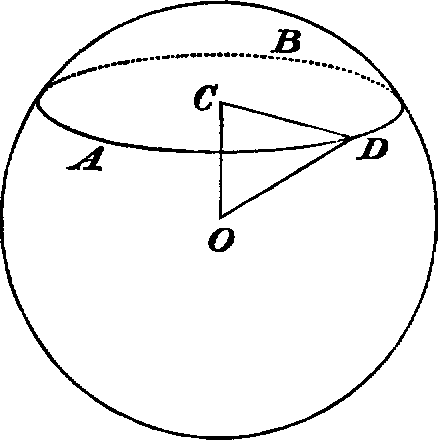
\includegraphics[width=5cm]{images/011fc}
\end{figure}

Let $AB$ be the section of the surface of a sphere made by any
plane, $O$ the centre of the sphere. Draw $OC$ perpendicular to the
plane; take any point $D$ in the section and join $OD$, $CD$. Since
$OC$ is perpendicular to the plane, the angle $OCD$ is a right angle;
therefore $CD=\surd(OD^2-OC^2)$. Now $O$ and $C$ are fixed points, so
that $OC$ is constant; and $OD$ is constant, being the radius of the
%-----File: 012.png------------------------------------------------
sphere; hence $CD$ is constant. Thus all points in the plane section
are equally distant from the fixed point $C$; therefore the section
is a circle of which $C$ is the centre.

\paragraph{3.} The section of the surface of a sphere by a plane is called
a \textit{great circle} if the plane passes through the centre of the sphere,
and a \textit{small circle} if the plane does not pass through the centre of
the sphere. Thus the radius of a great circle is equal to the
radius of the sphere.

\paragraph{4.} Through the centre of a sphere and any two points on the
surface a plane can be drawn; and only one plane can be drawn,
except when the two points are the extremities of a diameter of
the sphere, and then an infinite number of such planes can be
drawn. Hence only one great circle can be drawn through two
given points on the surface of a sphere, except when the points are
the extremities of a diameter of the sphere. When only one great
circle can be drawn through two given points, the great circle is
unequally divided at the two points; we shall for brevity speak of
the shorter of the two arcs as \textit{the} arc of a great circle joining the
two points.

\paragraph{5.} The \textit{axis} of any circle of a sphere is that diameter of the
sphere which is perpendicular to the plane of the circle; the extremities
of the axis are called the \textit{poles} of the circle. The poles
of a great circle are equally distant from the plane of the circle.
The poles of a small circle are not equally distant from the plane
of the circle; they may be called respectively the \textit{nearer} and \textit{further}
pole; sometimes the nearer pole is for brevity called \textit{the} pole.

\paragraph{6.} \textit{A pole of a circle is equally distant from every point of the
circumference of the circle.}

Let $O$ be the centre of the sphere, $AB$ any circle of the sphere,
$C$ the centre of the circle, $P$ and $P'$ the poles of the circle. Take
any point $D$ in the circumference of the circle; join $CD$, $OD$, $PD$.
Then $PD=\surd(PC^2+CD^2)$; and $PC$ and $CD$ are constant, therefore
$PD$ is constant. Suppose a great circle to pass through the points
$P$ and $D$; then the chord $PD$ is constant, and therefore the arc of
%-----File: 013.png------------------------------------------------
a great circle intercepted between $P$ and $D$ is constant for all
positions of $D$ on the circle $AB$.
\begin{figure}[htp]
\centering
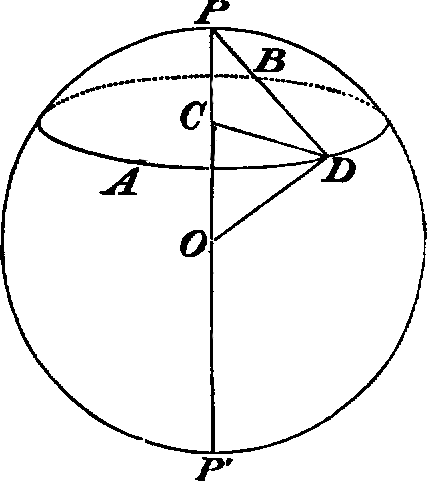
\includegraphics[width=5cm]{images/013f1c}
\end{figure}

Thus the distance of a pole of a circle from every point of the
circumference of the circle is constant, whether that distance be
measured by the straight line joining the points, or by the arc of
a great circle intercepted between the points.

\paragraph{7.} \textit{The arc of a great circle which is drawn from a pole of a
great circle to any point in its circumference is a quadrant.}
\begin{figure}[htp]
\centering
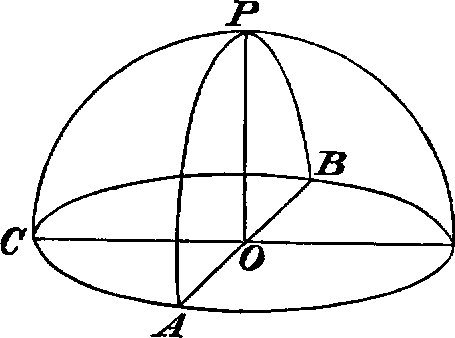
\includegraphics[width=5cm]{images/013f2c}
\end{figure}

Let $P$ be a pole of the great circle $ABC$; then the arc $PA$ is a
quadrant.

For let $O$ be the centre of the sphere, and draw $PO$. Then
$PO$ is at right angles to the plane $ABC$, because $P$ is the pole of
$ABC$, therefore $POA$ is a right angle, and the arc $PA$ is a quadrant.
%-----File: 014.png------------------------------------------------

\paragraph{8.} \textit{The angle subtended at the centre of a sphere by the arc of
a great circle which joins the poles of two great circles is equal to the
inclination of the planes of the great circles.}
\begin{figure}[htp]
\centering
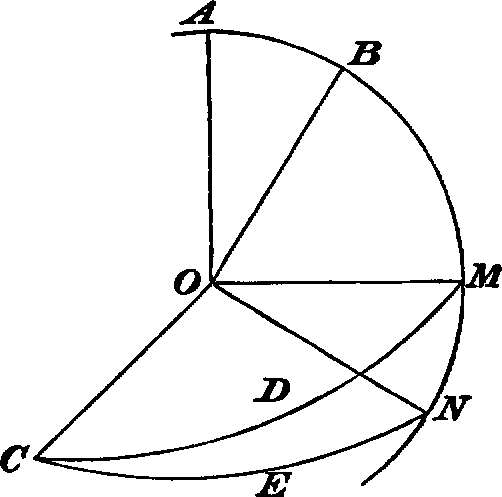
\includegraphics[width=5cm]{images/014fc}
\end{figure}

Let $O$ be the centre of the sphere, $CD$, $CE$ the great circles intersecting
at $C$, $A$ and $B$ the poles of $CD$ and $CE$ respectively.

Draw a great circle through $A$ and $B$, meeting $CD$ and $CE$ at
$M$ and $N$ respectively. Then $AO$ is perpendicular to $OC$, which is
a straight line in the plane $OCD$; and $BO$ is perpendicular to $OC$,
which is a straight line in the plane $OCE$; therefore $OC$ is perpendicular
to the plane $AOB$ (Euclid, \textsc{xi}.~4); and therefore $OC$ is
perpendicular to the straight lines $OM$ and $ON$, which are in the
plane $AOB$. Hence $MON$ is the angle of inclination of the planes
$OCD$ and $OCE$. And the angle
\[
AOB = AOM - BOM = BON - BOM = MON.
\]

\paragraph{9.} By the angle between two great circles is meant \textit{the angle
of inclination of the planes of the circles}. Thus, in the figure of
the preceding Article, the angle between the great circles $CD$ and
$CE$ is the angle $MON$.

In the figure to Art.~6, since $PO$ is perpendicular to the plane
$ACB$, every plane which contains $PO$ is at right angles to the
plane $ACB$. Hence the angle between the plane of any circle
and the plane of a great circle which passes through its poles is
a right angle.
%-----File: 015.png------------------------------------------------

\paragraph{10.} \textit{Two great circles bisect each other.}

For since the plane of each great circle passes through the
centre of the sphere, the line of intersection of these planes is a
diameter of the sphere, and therefore also a diameter of each great
circle; therefore the great circles are bisected at the points where
they meet.

\paragraph{11.} \textit{If the arcs of great circles joining a point $\mathrm{P}$ on the surface
of a sphere with two other points $\mathrm{A}$ and $\mathrm{C}$ on the surface of the
sphere, which are not at opposite extremities of a diameter, be each of
them equal to a quadrant, $\mathrm{P}$ is a pole of the great circle through
$\mathrm{A}$ and $\mathrm{C}$.} (See the figure of Art.~7.)

For suppose $PA$ and $PC$ to be quadrants, and $O$ the centre of
the sphere; then since $PA$ and $PC$ are quadrants, the angles $POC$
and $POA$ are right angles. Hence $PO$ is at right angles to the
plane $AOC$, and $P$ is a pole of the great circle $AC$.

\paragraph{12.} Great circles which pass through the poles of a great
circle are called \textit{secondaries} to that circle. Thus, in the figure of
Art.~8 the point $C$ is a pole of $ABMN$, and therefore $CM$ and $CN$
are parts of secondaries to $ABMN$. And the angle between $CM$
and $CN$ is measured by $MN$; that is, \textit{the angle between any two
great circles is measured by the arc they intercept on the great circle
to which they are secondaries.}

\paragraph{13.} \textit{If from a point on the surface of a sphere there can be
drawn two arcs of great circles, not parts of the same great circle,
the planes of which are at right angles to the plane of a given circle,
that point is a pole of the given circle.}

For, since the planes of these arcs are at right angles to the
plane of the given circle, the line in which they intersect is perpendicular
to the plane of the given circle, and is therefore the
axis of the given circle; hence the point from which the arcs are
drawn is a pole of the circle.
%-----File: 016.png------------------------------------------------

\paragraph{14.} \textit{To compare the arc of a small circle subtending any angle
at the centre of the circle with the arc of a great circle subtending
the same angle at its centre.}
\begin{figure}[htp]
\centering
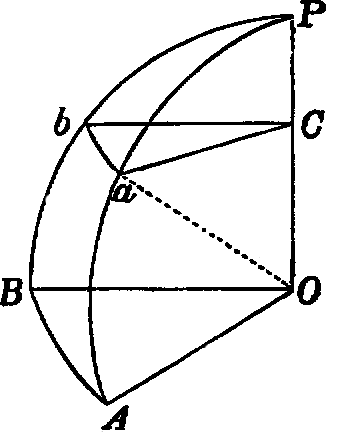
\includegraphics[width=5.0cm]{images/016fc}
\end{figure}

Let $ab$ be the arc of a small circle, $C$ the centre of the circle,
$P$ the pole of the circle, $O$ the centre of the sphere. Through $P$
draw the great circles $PaA$ and $PbB$, meeting the great circle
of which $P$ is a pole, at $A$ and $B$ respectively; draw $Ca$, $Cb$, $OA$,
$OB$. Then $Ca$, $Cb$, $OA$, $OB$ are all perpendicular to $OP$, because
the planes $aCb$ and $AOB$ are perpendicular to $OP$; therefore $Ca$
is parallel to $OA$, and $Cb$ is parallel to $OB$. Therefore the angle
$aCb=\text{the angle }AOB$ (Euclid, \textsc{xi}.\ 10). Hence,
\[
  \frac{\operatorname{arc} ab} {\operatorname{radius} Ca}=\frac{\operatorname{arc} AB} {\operatorname{radius} OA},
  \text{ (\textit{Plane Trigonometry}, Art.\ 18)};
\]
therefore,\hfill
$\displaystyle \frac{\operatorname{arc} ab}{\operatorname{arc} AB}=\frac{Ca}{OA}
=\frac{Ca}{Oa}=\sin POa$.\hfill\phantom{\text{therefore,}}

\chapter[Spherical Triangles.]{SPHERICAL TRIANGLES.}

\paragraph{15.} Spherical Trigonometry investigates the relations which
subsist between the angles of the plane faces which form a solid
angle and the angles at which the plane faces are inclined to each
other.
%-----File: 017.png------------------------------------------------

\paragraph{16.} Suppose that the angular point of a solid angle is made
the centre of a sphere; then the planes which form the solid angle
will cut the sphere in arcs of great circles. Thus a figure will be
formed on the surface of the sphere which is called a \textit{spherical
triangle} if it is bounded by \textit{three} arcs of great circles; this will be
the case when the solid angle is formed by the meeting of \textit{three}
plane angles. If the solid angle be formed by the meeting of
\textit{more than three} plane angles, the corresponding figure on the
surface of the sphere is bounded by more than three arcs of great
circles, and is called a \textit{spherical polygon}.

\paragraph{17.} The three arcs of great circles which form a spherical
triangle are called the \textit{sides} of the spherical triangle; the angles
formed by the arcs at the points where they meet are called the
\textit{angles} of the spherical triangle. (See Art.~9.)

\paragraph{18.} Thus, let $O$ be the centre of a sphere, and suppose a solid
angle formed at $O$ by the meeting of three plane angles. Let
\begin{figure}[htp]
\centering
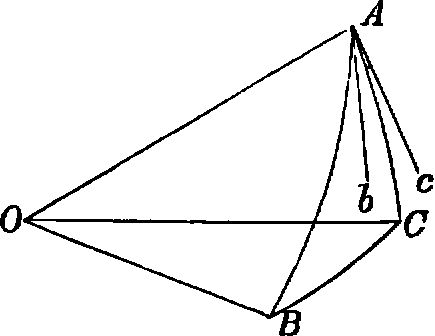
\includegraphics[width=5.0cm]{images/017fc}
\end{figure}
$AB$, $BC$, $CA$ be the arcs of great circles in which the planes cut
the sphere; then $ABC$ is a spherical triangle, and the arcs $AB$,
$BC$, $CA$ are its sides. Suppose $Ab$ the tangent at $A$ to the arc
$AB$, and $Ac$ the tangent at $A$ to the arc $AC$, the tangents being
drawn from $A$ \textit{towards} $B$ and $C$ respectively; then the angle $bAc$
is one of the angles of the spherical triangle. Similarly angles
formed in like manner at $B$ and $C$ are the other angles of the
spherical triangle.
%-----File: 018.png------------------------------------------------

\paragraph{19.} The principal part of a treatise on Spherical Trigonometry
consists of theorems relating to spherical triangles; it is therefore
necessary to obtain an accurate conception of a spherical triangle
and its parts.

It will be seen that what are called \textit{sides} of a spherical
triangle are really \textit{arcs} of great circles, and these arcs are proportional
to the three plane angles which form the solid angle
corresponding to the spherical triangle. Thus, in the figure of
the preceding Article, the arc $AB$ forms one side of the spherical
triangle $ABC$, and the plane angle $AOB$ is measured by the fraction
$\dfrac{\operatorname{arc} AB} {\operatorname{radius} OA}$; and thus the arc $AB$ is proportional to the angle
$AOB$ so long as we keep to the same sphere.

The \textit{angles} of a spherical triangle are the inclinations of the
plane faces which form the solid angle; for since $Ab$ and $Ac$ are
both perpendicular to $OA$, the angle $bAc$ is the angle of inclination
of the planes $OAB$ and $OAC$.

\paragraph{20.} The letters $A$, $B$, $C$ are generally used to denote the
\textit{angles} of a spherical triangle, and the letters $a$, $b$, $c$ are used to
denote the \textit{sides}. As in the case of plane triangles, $A$, $B$, and $C$
may be used to denote the numerical values of the angles expressed
in \textit{terms of any unit}, provided we understand distinctly what the
unit is. Thus, if the angle $C$ be a right angle, we may say that
$C = 90^\circ$, or that $C = \dfrac{\pi}{2}$, according as we adopt for the unit a degree
or the angle subtended at the centre by an arc equal to the
radius. So also, as the sides of a spherical triangle are proportional
to the angles subtended at the centre of the sphere, we
may use $a$, $b$, $c$ to denote the numerical values of those angles
in terms of any unit. We shall usually suppose both the angles
and sides of a spherical triangle expressed in \textit{circular measure}.
(\textit{Plane Trigonometry}, Art.\ 20.)
%-----File: 019.png------------------------------------------------

\paragraph{21.} In future, unless the contrary be distinctly stated, any
arc drawn on the surface of a sphere will be supposed to be an arc
of a \textit{great} circle.

\paragraph{22.} In spherical triangles each side is restricted to be less
than a semicircle; this is of course a \textit{convention}, and it is adopted
because it is found convenient.
\begin{figure}[htp]
\centering
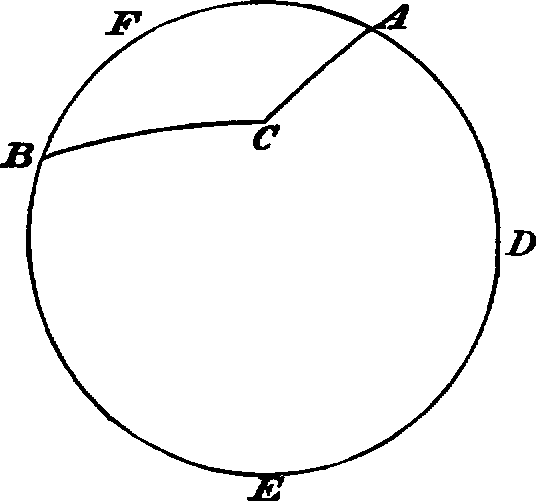
\includegraphics[width=5.0cm]{images/019fc}
\end{figure}

Thus, in the figure, the arc $ADEB$ is greater than a semicircumference,
and we might, if we pleased, consider $ADEB$, $AC$,
and $BC$ as forming a triangle, having its angular points at $A$, $B$,
and $C$. But we agree to exclude such triangles from our consideration;
and the triangle having its angular points at $A$, $B$,
and $C$, will be understood to be that formed by $AFB$, $BC$, and $CA$.

\paragraph{23.} From the restriction of the preceding Article it will
follow that \textit{any angle of a spherical triangle is less than two right
angles}.

For suppose a triangle formed by $BC$, $CA$, and $BEDA$, having
the angle $BCA$ greater than two right angles. Then suppose $D$
to denote the point at which the arc $BC$, if produced, will meet
$AE$; then $BED$ is a semicircle by Art.\ 10, and therefore $BEA$
is greater than a semicircle; thus the proposed triangle is not one
of those which we consider.
%-----File: 020.png------------------------------------------------

\chapter[Spherical Geometry.]{SPHERICAL GEOMETRY.}

\paragraph{24.} The relations between the sides and angles of a Spherical
Triangle, which are investigated in treatises on Spherical Trigonometry,
are chiefly such as involve the \textit{Trigonometrical Functions}
of the sides and angles. Before proceeding to these, however, we
shall collect, under the head of Spherical Geometry, some theorems
which involve the sides and angles \textit{themselves}, and not their trigonometrical
ratios.

\paragraph{25.} \textit{Polar triangle}. Let $ABC$ be any spherical triangle, and
let the points $A'$, $B'$, $C'$ be those poles of the arcs $BC$, $CA$, $AB$
\begin{figure}[htp]
\centering
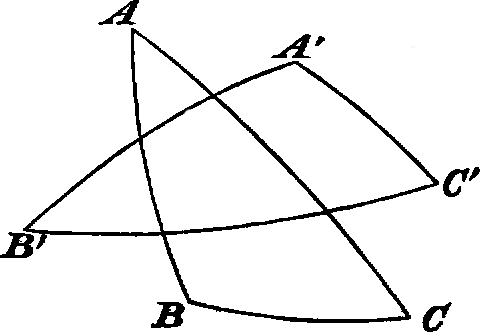
\includegraphics[width=5.0cm]{images/020fc}
\end{figure}
respectively which lie on the same sides of them as the opposite
angles $A$, $B$, $C$; then the triangle $A'B'C'$ is said to be the \textit{polar
triangle} of the triangle $ABC$.

Since there are two poles for each side of a spherical triangle,
\textit{eight} triangles can be formed having for their angular points poles
of the sides of the given triangle; but there is only one triangle in
which these poles $A'$, $B'$, $C'$ lie towards the same parts with the
corresponding angles $A$, $B$, $C$; and this is the triangle which is
known under the name of the \textit{polar triangle}.

The triangle $ABC$ is called the \textit{primitive} triangle with respect
to the triangle $A'B'C'$.
%-----File: 021.png------------------------------------------------

\paragraph{26.} \textit{If one triangle be the polar triangle of another, the latter
will be the polar triangle of the former.}

Let $ABC$ be any triangle, $A'B'C'$ the polar triangle: then $ABC$
will be the polar triangle of $A'B'C'$.
\begin{figure}[htp]
\centering
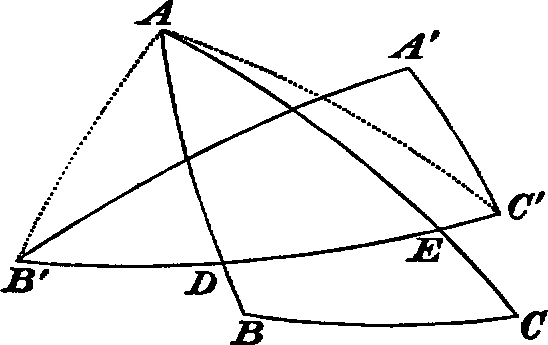
\includegraphics[width=5.0cm]{images/021fc}
\end{figure}

For since $B'$ is a pole of $AC$, the arc $AB'$ is a quadrant, and
since $C'$ is a pole of $BA$, the arc $AC'$ is a quadrant (Art.\ 7); therefore
$A$ is a pole of $B'C'$ (Art.\ 11). Also $A$ and $A'$ are on the same
side of $B'C'$; for $A$ and $A'$ are by hypothesis on the same side of
$BC$, therefore $A'A$ is less than a quadrant; and since $A$ is a pole
of $B'C'$, and $AA'$ is less than a quadrant, $A$ and $A'$ are on the
same side of $B'C'$.

Similarly it may be shewn that $B$ is a pole of $C'A'$, and that $B$
and $B'$ are on the same side of $C'A'$; also that $C$ is a pole of $A'B'$,
and that $C$ and $C'$ are on the same side of $A'B'$. Thus $ABC$ is the
polar triangle of $A'B'C'$.

\paragraph{27.} \textit{The sides and angles of the polar triangle are respectively
the supplements of the angles and sides of the primitive triangle.}

For let the arc $B'C'$, produced if necessary, meet the arcs $AB$,
$AC$, produced if necessary, at the points $D$ and $E$ respectively;
then since $A$ is a pole of $B'C'$, the spherical angle $A$ is measured by
the arc $DE$ (Art.\ 12). But $B'E$ and $C'D$ are each quadrants;
therefore $DE$ and $B'C'$ are together equal to a semicircle; that is,
the angle subtended by $B'C'$ at the centre of the sphere is the
%-----File: 022.png------------------------------------------------
supplement of the angle $A$. This we may express for shortness
thus; $B'C'$ is the supplement of $A$. Similarly it may be shewn
that $C'A'$ is the supplement of $B$, and $A'B'$ the supplement of $C$.

And since $ABC$ is the polar triangle of $A'B'C'$, it follows that
$BC$, $CA$, $AB$ are respectively the supplements of $A'$, $B'$, $C'$; that
is, $A'$, $B'$, $C'$ are respectively the supplements of $BC$, $CA$, $AB$.

From these properties a primitive triangle and its polar triangle
are sometimes called \textit{supplemental triangles}.

Thus, if $A$, $B$, $C$, $a$, $b$, $c$ denote respectively the angles and
the sides of a spherical triangle, all expressed in circular measure,
and $A'$, $B'$, $C'$, $a'$, $b'$, $c'$ those of the polar triangle, we have
\begin{align*}
A' &= \pi - a,& B' &= \pi - b,& C' &= \pi - c,\\
a' &= \pi - A,& b' &= \pi - B,& c' &= \pi - C.
\end{align*}

\paragraph{28.} The preceding result is of great importance; for if any
general theorem be demonstrated with respect to the sides and the
angles of any spherical triangle it holds of course for the polar
triangle also. \textit{Thus any such theorem will remain true when the
angles are changed into the supplements of the corresponding sides
and the sides into the supplements of the corresponding angles.} We
shall see several examples of this principle in the next Chapter.

\paragraph{29.} \textit{Any two sides of a spherical triangle are together greater
than the third side.} (See the figure of Art.\ 18.)

For any two of the three plane angles which form the solid
angle at $O$ are together greater than the third (Euclid, \textsc{xi}.\ 20).
Therefore any two of the arcs $AB$, $BC$, $CA$, are together greater
than the third.

From this proposition it is obvious that any side of a spherical
triangle is greater than the difference of the other two.

\paragraph{30.} \textit{The sum of the three sides of a spherical triangle is less than
the circumference of a great circle.} (See the figure of Art.\ 18.)
%-----File: 023.png------------------------------------------------

For the sum of the three plane angles which form the solid
angle at $O$ is less than four right angles (Euclid, \textsc{xi.}~21); therefore
\[
\dfrac{AB}{OA} + \dfrac{BC}{OA} + \dfrac{CA}{OA} \text{ is less than } 2\pi,
\]
therefore,\hfill
$\displaystyle AB+BC+CD \text{ is less than } 2\pi\times OA;$\hfill\phantom{\text{therefore}}\\
that is, the sum of the arcs is less than the circumference of a
great circle.

\paragraph{31.} The propositions contained in the preceding two Articles
may be extended. Thus, if there be any polygon which has each
of its angles less than two right angles, \textit{any one side is less than the
sum of all the others.} This may be proved by repeated use of
Art.~29. Suppose, for example, that the figure has four sides, and
let the angular points be denoted by $A$, $B$, $C$, $D$. Then
\[
AD+BC\text{ is greater than }AC;
\]
therefore,\hfill
$\displaystyle AB+BC+CD \text{ is greater than } AC+CD,$\hfill\phantom{\text{therefore}}\\
and \textit{{\`a} fortiori} greater than $AD$.

Again, if there be any polygon which has each of its angles
less than two right angles, \textit{the sum of its sides will be less than the
circumference of a great circle}. This follows from Euclid, \textsc{xi.}~21,
in the manner shewn in Art.~30.

\paragraph{32.} \textit{The three angles of a spherical triangle are together greater
than two right angles and less than six right angles.}

Let $A$, $B$, $C$ be the \textit{angles} of a spherical triangle; let $a'$, $b'$, $c'$
be the \textit{sides} of the polar triangle. Then by Art.~30,
\[
a'+b'+c'\text{ is less than }2\pi,
\]
that is,\hfill
$\displaystyle \pi-A+\pi-B+\pi-C\text{ is less than }2\pi;$\hfill{\phantom{that is}}\\
therefore,\hfill
$\displaystyle A+B+C\text{ is greater than }\pi$.\hfill\phantom{\text{therefore}}\\

And since each of the angles $A$, $B$, $C$ is less than $\pi$, the sum
$A+B+C$ is less than $3\pi$.
%-----File: 024.png------------------------------------------------

\paragraph{33.} \textit{The angles at the base of an isosceles spherical triangle are
equal.}
\begin{figure}[htp]
\centering
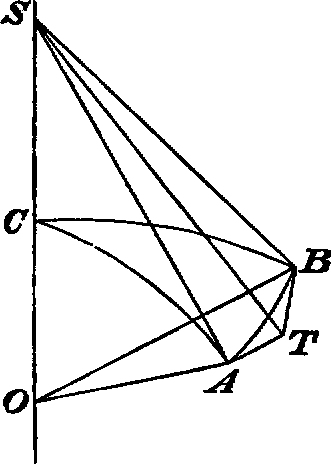
\includegraphics[width=5.0cm]{images/024fc}
\end{figure}

Let $ABC$ be a spherical triangle having $AC=BC$; let $O$ be the
centre of the sphere. Draw tangents at the points $A$ and $B$ to the
arcs $AC$ and $BC$ respectively; these will meet $OC$ produced at the
same point $S$, and $AS$ will be equal to $BS$.

Draw tangents $AT$, $BT$ at the points $A$, $B$ to the arc $AB$; then
$AT=TB$; join $TS$. In the two triangles $SAT$, $SBT$ the sides
$SA$, $AT$, $TS$ are equal to $SB$, $BT$, $TS$ respectively; therefore the
angle $SAT$ is equal to the angle $SBT$; and these are the angles at
the base of the spherical triangle.

The figure supposes $AC$ and $BC$ to be less than quadrants; if
they are greater than quadrants the tangents to $AC$ and $BC$ will
meet on $CO$ produced through $O$ instead of through $C$, and the
demonstration may be completed as before. If $AC$ and $BC$ are
quadrants, the angles at the base are right angles by Arts.~11
and 9.

\paragraph{34.} \textit{If two angles of a spherical triangle are equal, the opposite
sides are equal.}

Since the primitive triangle has two equal angles, the polar
triangle has two equal sides; therefore in the polar triangle the
angles opposite the equal sides are equal by Art.~33. Hence in
the primitive triangle the sides opposite the equal angles are
equal.
%-----File: 025.png------------------------------------------------

\paragraph{35.} \textit{If one angle of a spherical triangle be greater than another,
the side opposite the greater angle is greater than the side
opposite the less angle.}
\begin{figure}[htp]
\centering
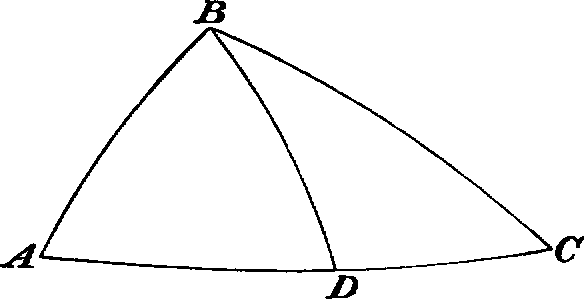
\includegraphics[width=5.0cm]{images/025fc}
\end{figure}

Let $ABC$ be a spherical triangle, and let the angle $ABC$ be
greater than the angle $BAC$: then the side $AC$ will be greater
than the side $BC$. At $B$ make the angle $ABD$ equal to the angle
$BAD$; then $BD$ is equal to $AD$ (Art.\ 34), and $BD+DC$ is greater
than $BC$ (Art.\ 29); therefore $AD+DC$ is greater than $BC$; that
is, $AC$ is greater than $BC$.

\paragraph{36.} \textit{If one side of a spherical triangle be greater than another,
the angle opposite the greater side is greater than the angle opposite
the less side.}

This follows from the preceding Article by means of the polar
triangle.

Or thus; suppose the side $AC$ greater than the side $BC$, then
the angle $ABC$ will be greater than the angle $BAC$. For the
angle $ABC$ cannot be less than the angle $BAC$ by Art.\ 35, and
the angle $ABC$ cannot be equal to the angle $BAC$ by Art.\ 34;
therefore the angle $ABC$ must be greater than the angle $BAC$.

This Chapter might be extended; but it is unnecessary to do
so because the Trigonometrical formul\ae\ of the next Chapter supply
an easy method of investigating the theorems of Spherical
Geometry. See Arts.\ 56, 57, and 58.
%-----File: 026.png------------------------------------------------

\chapter{Relations between the Trigonometrical
Functions of the Sides and the Angles
of a Spherical Triangle.}
\chaptermark{RELATIONS BETWEEN THE FUNCTIONS.}

\paragraph{37.} \textit{To express the cosine of an angle of a triangle in terms of
sines and cosines of the sides.}
\begin{figure}[htp]
\centering
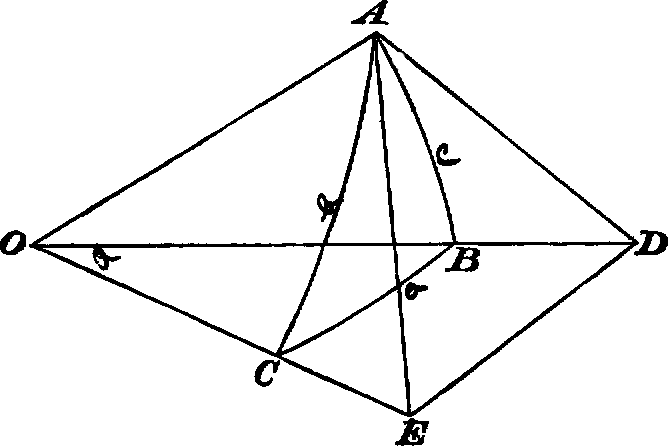
\includegraphics[width=5.0cm]{images/026fc}
\end{figure}

Let $ABC$ be a spherical triangle, $O$ the centre of the sphere.
Let the tangent at $A$ to the arc $AC$ meet $OC$ produced at $E$, and
let the tangent at $A$ to the arc $AB$ meet $OB$ produced at $D$; join
$ED$. Thus the angle $EAD$ is the angle $A$ of the spherical triangle,
and the angle $EOD$ measures the side $a$.

From the triangles $ADE$ and $ODE$ we have
\begin{align*}
DE^2 &= AD^2 + AE^2 - 2AD \centerdot AE \cos A,\\
DE^2 &= OD^2 + OE^2 - 2OD \centerdot OE \cos a;
\end{align*}
also the angles $OAD$ and $OAE$ are right angles, so that
$OD^2 = OA^2 + AD^2$ and $OE^2 = OA^2 + AE^2$. Hence by subtraction
we have
\begin{flalign*}
\multispan6{\hfil$0 = 2OA^2 + 2AD \centerdot AE \cos A - 2OD \centerdot OE \cos a$;\hfil}\\[1ex]
&\text{therefore}& \cos a
&= \dfrac{OA}{OE} \centerdot \dfrac{OA}{OD}
 + \dfrac{AE}{OE} \centerdot \dfrac{AD}{OD} \cos A;
&\phantom{\text{therefore}}&\\[1ex]
%
&\text{that is}& \cos a &= \cos b \cos c + \sin b \sin c \cos A.\\[1ex]
%
&\text{\indent Therefore}& \multispan{2}{\hfil$\cos A = \dfrac{\cos a - \cos b \cos c}{\sin b \sin c}$.\hfil}
\end{flalign*}
%-----File: 027.png------------------------------------------------

\paragraph{38.} We have supposed, in the construction of the preceding
Article, that the sides which contain the angle $A$ are less than
quadrants, for we have assumed that the tangents at $A$ meet $OB$
and $OC$ respectively produced. We must now shew that the
formul\ae\ obtained is true when these sides are not less than quadrants.
This we shall do by special examination of the cases in
which one side or each side is greater than a quadrant or equal to
a quadrant.

(1) Suppose only one of the sides which contain the angle $A$
to be greater than a quadrant, for example, $AB$. Produce $BA$
and $BC$ to meet at $B'$; and put $AB' = c'$, $CB' = a'$.
\begin{figure}[htp]
\centering
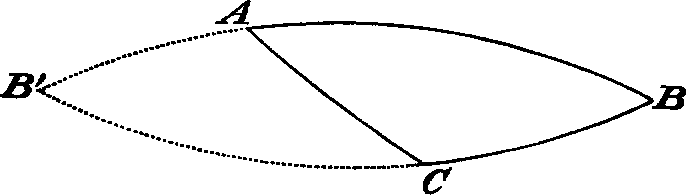
\includegraphics[width=5.0cm]{images/027f1c}
\end{figure}

Then we have from the triangle $AB'C$, by what has been
already proved,
\[
  \cos a' = \cos b \cos c' + \sin b \sin c' \cos B'AC;
\]
but $a' = \pi - a$, $c' = \pi - c$, $B'AC = \pi - A$; thus
\[
  \cos a = \cos b \cos c + \sin b \sin c \cos A.
\]

(2) Suppose both the sides which contain the angle $A$ to be
greater than quadrants. Produce $AB$ and $AC$ to meet at $A'$; put
$A'B = c', A'C = b'$; then from the triangle $A'BC$, as before,
\begin{figure}[htp]
\centering
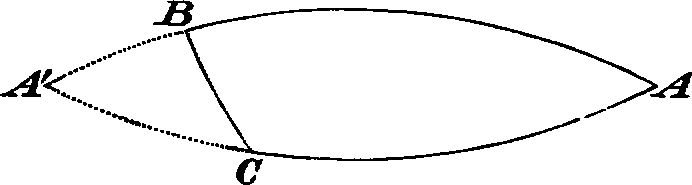
\includegraphics[width=5.0cm]{images/027f2c}
\end{figure}
\[
  \cos a = \cos b' \cos c' + \sin b' \sin c' \cos A';
\]
but $b' = \pi - b$, $c' = \pi - c$, $A' = A$; thus
\[
  \cos a = \cos b \cos c + \sin b \sin c \cos A.
\]
%-----File: 028.png------------------------------------------------

(3) Suppose that one of the sides which contain the angle $A$
is a quadrant, for example, $AB$; on $AC$, produced if necessary,
\begin{figure}[htp]
\centering
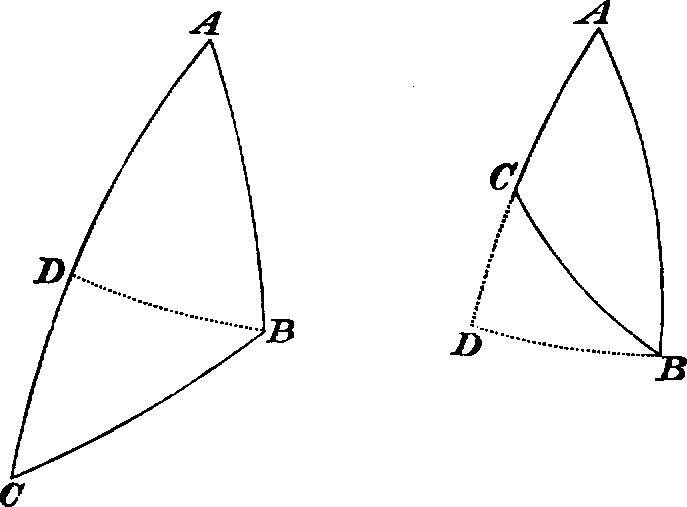
\includegraphics[width=5.0cm]{images/028fc}
\end{figure}
take $AD$ equal to a quadrant and draw $BD$. If $BD$ is a quadrant
$B$ is a pole of $AC$ (Art.\ 11); in this case $a = \dfrac{\pi}{2}$ and $A = \dfrac{\pi}{2}$ as well
as $c = \dfrac{\pi}{2}$. Thus the formula to be verified reduces to the identity
$0 = 0$. If $BD$ be not a quadrant, the triangle $BDC$ gives
\[
\cos a = \cos CD\cos BD + \sin CD\sin BD \cos CDB ,
\]
and \hfill$\ \cos CDB = 0,\ \
  \cos CD = \cos \left(\dfrac{\pi}{2} - b\right) = \sin b ,\ \
 \cos BD = \cos A $;\hfill\phantom{and}\\[1ex]
thus \hfill$ \cos a = \sin b \cos A ; $\hfill \phantom{thus}\\[2ex]
and this is what the formula in Art.\ 37 becomes when $c = \dfrac{\pi}{2}$.

(4) Suppose that both the sides which contain the angle $A$
are quadrants. The formula then becomes $\cos a = \cos A $; and this
is obviously true, for $A$ is now the pole of $BC$, and thus $A = a$.

Thus the formula in Art.\ 37 is proved to be universally true.
\paragraph{39.} The formula in Art.\ 37 may be applied to express the
cosine of any angle of a triangle in terms of sines and cosines of
the sides; thus we have the three formul\ae,
\begin{align*}
\cos a &= \cos b \cos c + \sin b \sin c \cos A,\\
\cos b &= \cos c \cos a + \sin c \sin a \cos B,\\
\cos c &= \cos a \cos b + \sin a \sin b \cos C.
\end{align*}
%-----File: 029.png------------------------------------------------
These may be considered as the fundamental equations of Spherical
Trigonometry; we shall proceed to deduce various formul\ae\
from them.

\paragraph{40.} \textit{To express the sine of an angle of a spherical triangle in
terms of trigonometrical functions of the sides.}
\begin{flalign*}
&\text{\indent We have}& \cos A&=\dfrac{\cos a-\cos b\cos c}{\sin b\sin c};\\[1.5ex]
%
&\text{therefore}& \sin^2 A&=1-\left(\dfrac{\cos a-\cos b\cos c}{\sin b\sin c}\right)^2\\[1.5ex]
%
&&&=\dfrac{(1-\cos^2 b)(1-\cos^2 c)-(\cos a-\cos b\cos c)^2}{\sin^2 b\sin^2 c}\\[1.5ex]
%
&&&=\dfrac{1-\cos^2 a-\cos^2 b-\cos^2 c+2\cos a\cos b\cos c}{\sin^2 b \sin^2 c};&\phantom{therefore}\\[1.5ex]
%
&\text{therefore} &\sin A&=\dfrac{\surd(1-\cos^2 a-\cos^2 b-\cos^2 c+2\cos a\cos b\cos c)}{\sin b \sin c}.
\end{flalign*}
The radical on the right-hand side must be taken with the positive
sign, because $\sin b$, $\sin c$, and $\sin A$ are all positive.

\paragraph{41.} From the value of $\sin A$ in the preceding Article it follows
that
\begin{gather*}
\dfrac{\sin A}{\sin a}=\dfrac{\sin B}{\sin b}=\dfrac{\sin C}{\sin c},\\
%
\intertext{for each of these is equal to the same expression, namely,}
%
\dfrac{\surd(1-\cos^2 a-\cos^2 b-\cos^2 c+2\cos a\cos b\cos c)}{\sin a\sin b\sin c}.
\end{gather*}
Thus \textit{the sines of the angles of a spherical triangle are proportional
to the sines of the opposite sides}. We will give an independent
proof of this proposition in the following Article.

\paragraph{42.} \textit{The sines of the angles of a spherical triangle are proportional
to the sines of the opposite sides.}
%-----File: 030.png------------------------------------------------

Let $ABC$ be a spherical triangle, $O$ the centre of the sphere.
Take any point $P$ in $OA$, draw $PD$ perpendicular to the plane
\begin{figure}[htp]
\centering
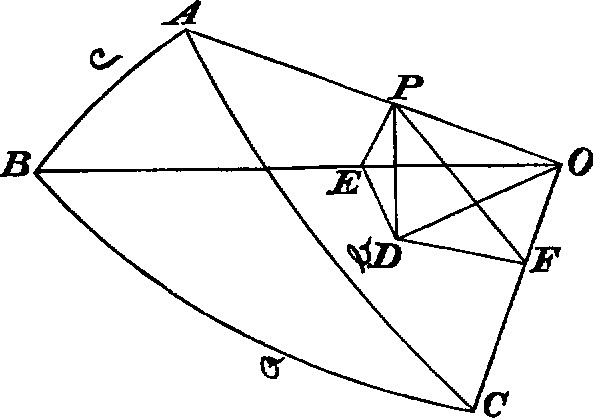
\includegraphics[width=5.0cm]{images/030fc}
\end{figure}
$BOC$, and from $D$ draw $DE$, $DF$ perpendicular to $OB$, $OC$ respectively;
join $PE$, $PF$, $OD$.

Since $PD$ is perpendicular to the plane $BOC$, it makes right
angles with every straight line meeting it in that plane; hence
\[
PE^2 = PD^2 + DE^2 = PO^2-OD^2 + DE^2 = PO^2-OE^2;
\]
thus $PEO$ is a right angle. Therefore $PE = OP\sin POE= OP \sin c$;
and $PD = PE \sin PED = PE \sin B = OP \sin c \sin B$.

Similarly, $PD = OP \sin b \sin C$; therefore
\begin{flalign*}
&&OP \sin c \sin B &= OP \sin b \sin C;\\
&\text{therefore} &\dfrac{\sin B}{\sin C}&=\dfrac{\sin b}{\sin c}.&\phantom{\text{therefore}}&
\end{flalign*}

The figure supposes $b$, $c$, $B$, and $C$ each less than a right angle;
it will be found on examination that the proof will hold when the
figure is modified to meet any case which can occur. If, for
instance, $B$ alone is greater than a right angle, the point $D$ will
fall beyond $OB$ instead of between $OB$ and $OC$; then $PED$ will
be the \textit{supplement} of $B$, and thus $\sin PED$ is still equal to $\sin B$.

\paragraph{43.} \textit{To shew that} $\cot a \sin b = \cot A \sin C + \cos b \cos C$.
\begin{flalign*}
&\text{\indent We have} &\cos a &= \cos b \cos c + \sin b \sin c \cos A,\\
&&\cos c &= \cos a \cos b + \sin a \sin b \cos C,\\
&&\sin c &= \sin a\,\dfrac{\sin C}{\sin A}.&\phantom{We have}
\end{flalign*}
%-----File: 031.png------------------------------------------------

Substitute the values of $\cos c$ and $\sin c$ in the first equation;
thus
\[
\cos a = (\cos a \cos b + \sin a \sin b \cos C) \cos b +
\dfrac{\sin a \sin b \cos A \sin C}{\sin A};
\]
by transposition
\[
\cos a \sin^2 b = \sin a \sin b \cos b \cos C + \sin a \sin b \cot A \sin C;
\]
divide by $\sin a \sin b$; thus
\[
\cot a \sin b = \cos b \cos C + \cot A \sin C.
\]

\paragraph{44.} By interchanging the letters five other formul\ae\ may be
obtained like that in the preceding Article; the whole six formul\ae\
will be as follows:
\begin{align*}
&\cot a \sin b = \cot A \sin C + \cos b \cos C, \\
&\cot b \sin a = \cot B \sin C + \cos a \cos C, \\
&\cot b \sin c = \cot B \sin A + \cos c \cos A, \\
&\cot c \sin b = \cot C \sin A + \cos b \cos A, \\
&\cot c \sin a = \cot C \sin B + \cos a \cos B, \\
&\cot a \sin c = \cot A \sin B + \cos c \cos B.
\end{align*}

\paragraph{45.} \textit{To express the sine, cosine, and tangent, of half an angle
of a triangle as functions of the sides.}

We have, by Art.~37, $\cos A = \dfrac{\cos a - \cos b \cos c}{\sin b \sin c}$;\\[1.5ex]
therefore\hfill
$\displaystyle 1 - \cos A = 1 - \dfrac{\cos a - \cos b \cos c}{\sin b \sin c} =
\dfrac{\cos (b - c) - \cos a}{\sin b \sin c};$\hfill\phantom{\text{therefore}}\\[2ex]
therefore\hfill
$\displaystyle \sin^2 \dfrac{A}{2} = \dfrac{\sin \tfrac{1}{2}(a+b-c)\sin\tfrac{1}{2}(a-b+c)}{\sin b \sin c}$.\hfill\phantom{\text{therefore}}\\

Let $2s = a + b + c$, so that $s$ is half the sum of the sides of
the triangle; then
\[
a + b - c = 2s - 2c = 2(s - c),\quad
a - b + c = 2s - 2b = 2(s - b);
\]
\begin{flalign*}
&\text{thus,} &
\sin^2 \dfrac{A}{2} &= \dfrac{\sin(s - b)\sin(s - c)}{\sin b \sin c}, &\phantom{\text{thus,}}\\
%-----File: 032.png------------------------------------------------
&\text{and}&
\sin\dfrac{A}{2}&=\Surd{\left\{
  \dfrac{\sin(s-b)\sin(s-c)}{\sin b \sin c}
  \right\}}
  &\phantom{\text{Also,}}\\[1ex]
&\text{Also,}&
1+\cos A &= 1+\dfrac{\cos a-\cos b\cos c}{\sin b \sin c}=
  \dfrac{\cos a-\cos(b+c)}{\sin b \sin c};
\end{flalign*}
therefore
\begin{flalign*}
&&
\cos^2\dfrac{A}{2} &=
  \dfrac{\sin\tfrac{1}{2}(a+b+c)\sin\tfrac{1}{2}(b+c-a)}{\sin b\sin c} =
  \dfrac{\sin s \sin(s-a)}{\sin b \sin c},&\phantom{\text{and}}\\[1.5ex]
&\text{and}&
\cos\dfrac{A}{2}&=\Surd{\left\{
  \dfrac{\sin s \sin(s-a)}{\sin b \sin c}\right\}}
\end{flalign*}

From the expressions for $\sin\dfrac{A}{2}$ and $\cos\dfrac{A}{2}$ we deduce
\[
\tan\dfrac{A}{2}=\Surd{\left\{
  \dfrac{\sin(s-b)\sin(s-c)}{\sin s \sin(s-a)} \right\}}.
\]

The positive sign must be given to the radicals which occur in
this Article, because $\dfrac{A}{2}$ is less than a right angle, and therefore its
sine, cosine, and tangent are all positive.

\paragraph{46.} Since $\sin A = 2 \sin \dfrac{A}{2} \cos \dfrac{A}{2}$, we obtain
\[
\sin A = \dfrac{2}{\sin b \sin c}\{\sin s \sin(s-a)\sin(s-b)\sin(s-c)\}^{\tfrac{1}{2}}.
\]

It may be shewn that the expression for $\sin A$ in Art.\ 40
agrees with the present expression by putting the numerator of
that expression in factors, as in \textit{Plane Trigonometry}, Art.\ 115.
We shall find it convenient to use a symbol for the radical in the
value of $\sin A$; we shall denote it by $n$, so that
\begin{flalign*}
&&n^2&=\sin s \sin(s-a)\sin(s-b)\sin(s-c),&\phantom{\text{and}}\\
&\text{and} &4n^2&=1-\cos^2 a-\cos^2 b - \cos^2 c + 2\cos a\cos b\cos c.
\end{flalign*}
%-----File: 033.png------------------------------------------------

\paragraph{47.} \textit{To express the cosine of a side of a triangle in terms of
sines and cosines of the angles.}

In the formula of Art.\ 37 we may, by Art.\ 28, change the
sides into the supplements of the corresponding angles and the
angle into the supplement of the corresponding side; thus
\begin{flalign*}
&&\multispan{2}{\hfil\clap{$\cos (\pi-A) = \cos (\pi-B) \cos (\pi-C)+\sin (\pi-B)\sin(\pi-C) \cos(\pi-a)$,}\hfil}\\
&\text{that is,}&\cos A &=-\cos B \cos C + \sin B \sin C \cos a.\\
&\text{Similarly}&\cos B &=-\cos C \cos A + \sin C \sin A \cos b,&\phantom{Similarly}&\\
&\text{and}&\cos C &=-\cos A \cos B + \sin A \sin B \cos c.
\end{flalign*}

\paragraph{48.} The formul\ae\ in Art.\ 44 will of course remain true when
the angles and sides are changed into the supplements of the corresponding
sides and angles respectively; it will be found, however,
that no \textit{new} formul\ae\ are thus obtained, but only the \textit{same}
formul\ae\ over again. This consideration will furnish some assistance
in retaining those formul\ae\ accurately in the memory.

\paragraph{49.} \textit{To express the sine, cosine, and tangent, of half a side of a
triangle as functions of the angles.}

We have, by Art.\ 47, $\cos a=\dfrac{\cos A + \cos B \cos C}{\sin B\sin C}$;
\begin{flalign*}
&\text{therefore}&\\
&&\multispan{2}{\hfil\clap{$\displaystyle1-\cos a= 1-\dfrac{\cos A + \cos B\cos C}{\sin B\sin C}= -\dfrac{\cos A+\cos(B+C)}{\sin B\sin C}$;}\hfil}\\[2ex]
&\text{therefore}&\sin^{2}\dfrac{a}{2}&= -\frac{\cos\tfrac{1}{2}(A+B+C)\cos\tfrac{1}{2}(B+C-A)}{\sin B\sin C}.&\phantom{therefore}&\\[2ex]
&\rlap{\indent Let $2S=A+B+C$; then $B+C-A=2(S-A)$, therefore}&\vphantom{\dfrac a2}\\
&&\multispan{2}{\hfil$\displaystyle\sin^{2}\frac{a}{2}=-\frac{\cos S\cos(S-A)}{\sin B\sin C}$,\hfil}\\[2ex]
&\text{and}&\multispan{2}{\hfil$\displaystyle\sin\frac{a}{2}=\Surd{\left\{-\dfrac{\cos S\cos(S-A)}{\sin B\sin C}\right\}}$.\hfil}
\end{flalign*}
%-----File: 034.png------------------------------------------------
Also\ \hfil$1+\cos a=1+\dfrac{\cos A + \cos B \cos C}{\sin B\sin C}=\dfrac{\cos A +\cos (B-C)}{\sin B\sin C}$;\hfil\break\\
therefore
\[
\cos^{2}\dfrac{a}{2}=
\dfrac{\cos\tfrac{1}{2}(A-B+C)\cos\tfrac{1}{2}(A+B-C)}{\sin B\sin C}=
\dfrac{\cos(S-B)\cos(S-C)}{\sin B\sin C},
\]
\begin{flalign*}
&\text{and}&\cos\dfrac{a}{2}&=\Surd{\left\{\dfrac{\cos(S-B)\cos(S-C)}{\sin B\sin C}\right\}}.\\[2ex]
&\text{Hence }&\tan\dfrac{a}{2}&=\Surd{\left\{-\dfrac{\cos S\cos(S-A)}{\cos(S-B)\cos(S-C)}\right\}}.&\phantom{Hence}&
\end{flalign*}

The positive sign must be given to the radicals which occur in
this Article, because $\dfrac{a}{2}$ is less than a right angle.

\paragraph{50.} The expressions in the preceding Article may also be
obtained immediately from those given in Art.\ 45 by means of
Art.\ 28.

It may be remarked that the values of $\sin\dfrac{a}{2}$, $\cos\dfrac{a}{2}$, and $\tan\dfrac{a}{2}$
are \textit{real}. For $S$ is greater than one right angle and less than three
right angles by Art.\ 32; therefore $\cos S$ is \textit{negative}. And in the
polar triangle any side is less than the sum of the other two; thus
$\pi-A$ is less than $\pi-B + \pi-C$; therefore $B + C - A$ is less than
$\pi$; therefore $S - A$ is less than $\dfrac{\pi}{2}$, and $B + C - A$ is algebraically
greater than $-\pi$, so that $S-A$ is algebraically greater than $-\dfrac{\pi}{2}$;
therefore $\cos (S-A)$ is \textit{positive}. Similarly also $\cos (S-B)$ and
$\cos (S-C)$ are positive. Hence the values of $\sin\dfrac{a}{2}$, $\cos\dfrac{a}{2}$, and $\tan\dfrac{a}{2}$
are real.

\paragraph{51.} Since $\sin a= 2 \sin\dfrac{a}{2}\cos\dfrac{a}{2}$, we obtain
\[
\sin a=\dfrac{2}{\sin B\sin C}\left\{-\cos S\cos (S-A)\cos(S-B)\cos (S-C)\right\}^{\tfrac{1}{2}}.
\]

We shall use $N$ for $\left\{-\cos S\cos (S-A)\cos(S-B)\cos (S-C)\right\}^{\tfrac{1}{2}}$.
%-----File: 035.png------------------------------------------------

\paragraph{52.} \textit{To demonstrate Napier's Analogies}.
\begin{flalign*}
&\rlap{\indent We have}&\multispan{2}{\hfil$\displaystyle\dfrac{\sin A}{\sin a} = \dfrac{\sin B}{\sin b} = m$ suppose;\hfil}\\
&\rlap{then, by a theorem of Algebra,}\\
&&m &= \dfrac{\sin A + \sin B}{\sin a + \sin b},\tag{1}\\[1ex]
&\rlap{and also}&m &= \dfrac{\sin A - \sin B}{\sin a - \sin b}.\tag{2}\\
&\text{Now}&\cos A + \cos B \cos C &= \sin B \sin C \cos a = m \sin C \sin b \cos a,&\phantom{Now}\\
&\text{and}&\cos B + \cos A \cos C &= \sin A \sin C \cos b = m \sin C \sin a \cos b,
\end{flalign*}
therefore, by addition,
\[
(\cos A + \cos B)(1 + \cos C) = m\sin C \sin (a + b);\tag{3}
\]
therefore by (1) we have
\begin{flalign*}
&&\dfrac{\sin A + \sin B}{\cos A + \cos B} &= \dfrac{\sin a + \sin b}{\sin(a + b)}\dfrac{1 + \cos C}{\sin C},\\[1ex]
&\text{that is,}&\tan\tfrac{1}{2}(A + B) &= \frac{\cos\tfrac{1}{2}(a - b)}{\cos\tfrac{1}{2}(a + b)}\cot\frac{C}{2}.\tag{4}&\phantom{that is,}&
\end{flalign*}

Similarly from (3) and (2) we have
\begin{flalign*}
&&\dfrac{\sin A - \sin B}
     {\cos A + \cos B} &=
\dfrac{\sin a - \sin b}
     {\sin(a + b)}\,
\dfrac{1 + \cos C}
     {\sin C},\\[1ex]
&\text{that is,}&\tan\frac{1}{2}(A - B) &=
\frac{\sin\tfrac{1}{2}(a - b)}
     {\sin\tfrac{1}{2}(a + b)}
      \cot\frac{C}{2}.\tag{5}&\phantom{that is,}
\end{flalign*}

By writing $\pi-A$ for $a$, and so on in (4) and (5) we obtain
\begin{align*}
\tan\tfrac{1}{2}(a + b) &=
\frac{\cos\tfrac{1}{2}(A - B)}
     {\cos\tfrac{1}{2}(A + B)}
      \tan\frac{c}{2},			\tag{6}\\[1ex]
\tan\tfrac{1}{2}(a - b) &=
\frac{\sin\tfrac{1}{2}(A - B)}
     {\sin\tfrac{1}{2}(A + B)}
      \tan\frac{c}{2}.			\tag{7}
\end{align*}

The formul\ae\ (4), (5), (6), (7) may be put in the form of proportions
or analogies, and are called from their discoverer \textit{Napier's
%-----File: 036.png------------------------------------------------
Analogies:} the last two may be demonstrated without recurring
to the polar triangle by starting with the formul\ae\ in Art.~39.

\paragraph{53.} In equation (4) of the preceding Article, $\cos\tfrac{1}{2}(a - b)$ and
$\cot\dfrac{C}{2}$ are necessarily positive quantities; hence the equation
shews that $\tan\tfrac{1}{2}(A + B)$ and $\cos\tfrac{1}{2}(a + b)$ are of the same sign;
thus $\tfrac{1}{2}(A+B)$ and $\tfrac{1}{2}(a + b)$ are either both less than a right angle or both greater than a right angle. This is expressed by saying
that $\tfrac{1}{2}(A+B)$ and $\tfrac{1}{2}(a + b)$ \textit{are of the same affection}.

\paragraph{54.} \textit{To demonstrate Delambre's Analogies.}

We have $\cos c = \cos a \cos b + \sin a \sin b \cos C$; therefore
\begin{align*}
1 + \cos c &= 1 + \cos a \cos b +
                  \sin a \sin b (\cos^2\tfrac{1}{2}C -
                                 \sin^2\tfrac{1}{2}C)\\
%
           &= \{1 + \cos (a - b)\} \cos^2\tfrac{1}{2}C +
              \{1 + \cos (a + b)\} \sin^2\tfrac{1}{2}C;
\end{align*}
therefore $\displaystyle%
    \cos^2\tfrac{1}{2}c =
    \cos^2\tfrac{1}{2}(a - b)
    \cos^2\tfrac{1}{2}C +
    \cos^2\tfrac{1}{2}(a + b)
    \sin^2\tfrac{1}{2}C$.
\\
Similarly, $\displaystyle%
    \sin^2\tfrac{1}{2}c =
    \sin^2\tfrac{1}{2}(a - b)
    \cos^2\tfrac{1}{2}C +
    \sin^2\tfrac{1}{2}(a + b)
    \sin^2\tfrac{1}{2}C$.

Now add unity to the square of each member of Napier's first
two analogies; hence by the formul\ae\ just proved
\begin{align*}
    \sec^{2}\tfrac{1}{2}(A + B) &=
        \frac{\cos^{2}\tfrac{1}{2}c}
        {\cos^{2}\tfrac{1}{2}(a + b)
        \sin^{2}\tfrac{1}{2}C},\\[1ex]
%
    \sec^{2}\tfrac{1}{2}(A - B) &=
        \frac{\sin^{2}\tfrac{1}{2}c}
        {\sin^{2}\tfrac{1}{2}(a + b)
        \sin^{2}\tfrac{1}{2}C}.
\end{align*}

Extract the square roots; thus, since $\frac{1}{2}(A + B)$ and $\frac{1}{2}(a + b)$
are of the same affection, we obtain
\begin{align*}
    \cos\tfrac{1}{2}(A + B)
    \cos\tfrac{1}{2}c &=
    \cos\tfrac{1}{2}(a + b)
    \sin\tfrac{1}{2}C, \tag{1}\\[2ex]
%
    \cos\tfrac{1}{2}(A - B)
    \sin\tfrac{1}{2}c &=
    \sin\tfrac{1}{2}(a + b)
    \sin\tfrac{1}{2}C. \tag{2}
\end{align*}

Multiply the first two of Napier's analogies respectively by
these results; thus
\begin{align*}
    \sin\tfrac{1}{2}(A + B)
    \cos\tfrac{1}{2}c &=
    \cos\tfrac{1}{2}(a - b)
    \cos\tfrac{1}{2}C, \tag{3}\\[2ex]
%
    \sin\tfrac{1}{2}(A - B)
    \sin\tfrac{1}{2}c &=
    \sin\tfrac{1}{2}(a - b)
    \cos\tfrac{1}{2}C. \tag{4}
\end{align*}
%-----File: 037.png------------------------------------------------

The last four formul\ae\ are commonly, but improperly, called
\textit{Gauss's Theorems}; they were first given by Delambre in the
\textit{Connaissance des Tems} for 1809, page~445. See the \textit{Philosophical
Magazine} for February, 1873.

\paragraph{55.} The properties of supplemental triangles were proved
geometrically in Art.~27, and by means of these properties the
formul\ae\ in Art.~47 were obtained; but these formul\ae\ may be
deduced analytically from those in Art.~39, and thus the whole
subject may be made to depend on the formul\ae\ of Art.~39.

For from Art.~39 we obtain expressions for $\cos A$, $\cos B$, $\cos C$;
and from these we find
\begin{multline*}
\cos A + \cos B \cos C \\
= \dfrac{(\cos a - \cos b \cos c) \sin^2 a + (\cos b - \cos a \cos c)(\cos c - \cos a \cos b)}
{\sin^2 a \sin b \sin c}.
\end{multline*}
In the numerator of this fraction write $1 - \cos^2 a$ for $\sin^2 a$; thus
the numerator will be found to reduce to
\[
\cos a (1 - \cos^2 a - \cos^2 b - \cos^2 c + 2\cos a \cos b \cos c),
\]
and this is equal to $\cos a \sin B \sin C \sin^2 a \sin b \sin c$, (Art.~41);\\
therefore \hfill $\cos A + \cos B \cos C - \cos a \sin B \sin C$.
\hfill\phantom{therefore}\\
Similarly the other two corresponding formul\ae\ may be proved.

Thus the formul\ae\ in Art.~47 are established; and therefore,
without assuming the existence and properties of the Polar Triangle,
we deduce the following theorem: \textit{If the sides and angles
of a spherical triangle be changed respectively into the supplements
of the corresponding angles and sides, the fundamental formul\ae\ of
Art.~39 hold good, and therefore also all results deducible from them.}

\paragraph{56.} The formul\ae\ in the present Chapter may be applied to
establish analytically various propositions respecting spherical triangles
which either have been proved geometrically in the preceding
Chapter, or may be so proved. Thus, for example, the
second of Napier's analogies is
\[
\tan \tfrac{1}{2}(A-B) =
\dfrac{\sin\tfrac{1}{2}(a-b)}{\sin\tfrac{1}{2}(a+b)}
\cot\dfrac{C}{2};
\]
%-----File: 038.png------------------------------------------------
this shews that $\tfrac{1}{2}(A - B)$ is positive, negative, or zero, according
as $\dfrac{1}{2}(a - b)$ is positive, negative, or zero; thus we obtain all the
results included in Arts.~33\ldots36.

\paragraph{57.} \textit{If two triangles have two sides of the one equal to two
sides of the other, each to each, and likewise the included angles
equal, then their other angles will be equal, each to each, and likewise
their bases will be equal.}

We may shew that the bases are equal by applying the first
formula in Art.~39 to each triangle, supposing $b$, $c$, and $A$ the
same in the two triangles; then the remaining two formul\ae\ of
Art.~39 will shew that $B$ and $C$ are the same in the two triangles.

It should be observed that the two triangles in this case are
\textit{not} necessarily such that one may be made to \textit{coincide with the
other by superposition}. The sides of one may be equal to those of
the other, each to each, but in a reverse order, as in the following
figures.
\begin{figure}[htp]
\centering
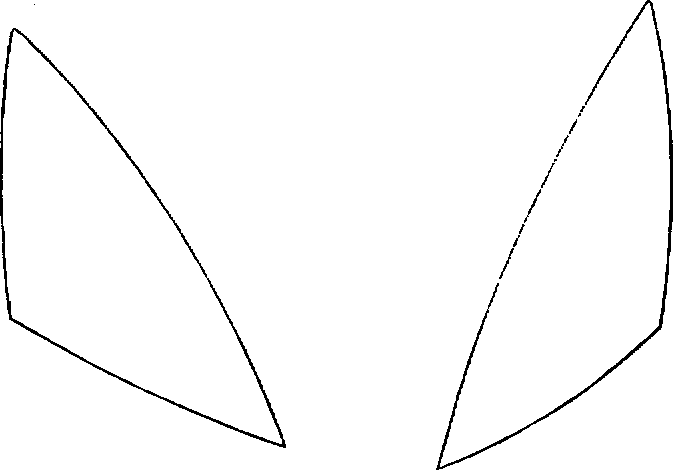
\includegraphics[width=5.0cm]{images/038fc}
\end{figure}

Two triangles which are equal in this manner are said to be
\textit{symmetrically} equal; when they are equal so as to admit of superposition
they are said to be \textit{absolutely} equal.

\paragraph{58.} \textit{If two spherical triangles have two sides of the one equal to
two sides of the other, each to each, but the angle which is contained
by the two sides of the one greater than the angle which is contained
by the two sides which are equal to them of the other, the base of that
%-----File: 039.png------------------------------------------------
which has the greater angle will be greater than the base of the
other; and conversely}.

Let $b$ and $c$ denote the sides which are equal in the two triangles;
let $a$ be the base and $A$ the opposite angle of one triangle,
and $a'$ and $A'$ similar quantities for the other. Then
\begin{align*}
  \cos a  &= \cos b \cos c + \sin b \sin c \cos A,\\
  \cos a' &= \cos b \cos c + \sin b \sin c \cos A';
\end{align*}
therefore \hfill
$\cos a - \cos a' + \sin b \sin c (\cos A - \cos A');$
\hfill\phantom{therefore}\\
that is,
\[
  \sin\tfrac{1}{2} (a + a')
  \sin\tfrac{1}{2} (a - a') =
  \sin b \sin c \sin\tfrac{1}{2} (A + A')
                \sin\tfrac{1}{2} (A - A');
\]
this shews that $\tfrac{1}{2} (a - a')$ and $\tfrac{1}{2} (A - A')$ are of the same sign.

\paragraph{59.} \textit{If on a sphere any point be taken within a circle which
is not its pole, of all the arcs which can be drawn from that point
to the circumference, the greatest is that in which the pole is, and the
other part of that produced is the least; and of any others, that which
is nearer to the greatest is always greater than one more remote; and
from the same point to the circumference there can be drawn only
two arcs which are equal to each other, and these make equal angles
with the shortest arc on opposite sides of it.}

This follows readily from the preceding three Articles.

\paragraph{60.} We will give another proof of the fundamental formul\ae\
in Art.~39, which is very simple, requiring only a knowledge of
the elements of Co-ordinate Geometry.

Suppose $ABC$ any spherical triangle, $O$ the centre of the
sphere, take $O$ as the origin of co-ordinates, and let the axis of $z$
pass through $C$. Let $x_1$, $y_1$, $z_1$ be the co-ordinates of $A$, and $x_2$,
$y_2$, $z_2$ those of $B$; let $r$ be the radius of the sphere. Then the
square on the straight line $AB$ is equal to
\[
  (x_1 - x_2)^2 +
  (y_1 - y_2)^2 +
  (z_1 - z_2)^2,
\]
and also to \hfill $r^2 + r^2 - 2r^2 \cos AOB;$
\hfill\phantom{and also to}\\[1ex]
%-----File: 040.png------------------------------------------------
and \ $x_1^2 + y_1^2 + z_1^2 = r^2$, $x_2^2 + y_2^2 + z_2^2 = r^2$, thus
\[
x_1x_2 + y_1y_2 + z_1z_2 = r^2 \cos AOB.
\]

Now make the usual substitutions in passing from rectangular
to polar co-ordinates, namely,
\begin{align*}
z_1 &= r \cos \theta_1, &x_1 &= r \sin \theta_1 \cos \phi_1, &y_1 &= r \sin \theta_1 sin \phi_1, \\
z_2 &= r \cos \theta_2, &x_2 &= r \sin \theta_2 \cos \phi_2, &y_2 &= r \sin \theta_2 sin \phi_2;
\end{align*}
thus we obtain
\[
\cos \theta_2 \cos \theta_1 + \sin \theta_2 \sin \theta_1 \cos (\phi_1 - \phi_2) = \cos AOB,
\]
that is, in the ordinary notation of Spherical Trigonometry,
\[
\cos a \cos b + \sin a \sin b \cos C = \cos c.
\]

This method has the advantage of giving a \textit{perfectly general
proof}, as all the equations used are universally true.

\section*{\centering\normalsize EXAMPLES.}

\indent 1. If $A = a$, shew that $B$ and $b$ are equal or supplemental, as
also $C$ and $c$.
\medskip

2. If one angle of a triangle be equal to the sum of the other
two, the greatest side is double of the distance of its middle point
from the opposite angle.
\medskip

3. When does the polar triangle coincide with the primitive
triangle?
\medskip

4. If $D$ be the middle point of $AB$, shew that
\[
\cos AC + \cos BC = 2 \cos \tfrac{1}{2} AB \cos CD.
\]

5. If two angles of a spherical triangle be respectively equal
to the sides opposite to them, shew that the remaining side is the
supplement of the remaining angle; or else that the triangle has
two quadrants and two right angles, and then the remaining side
is equal to the remaining angle.
%-----File: 041.png------------------------------------------------
\medskip

6. In an equilateral triangle, shew that $2 \cos \dfrac a2 \sin \dfrac A2 = 1$.
\medskip

7. In an equilateral triangle, shew that $\tan^2 \dfrac a2 = 1 - 2 \cos A$;\\
hence deduce the limits between which the sides and the angles of
an equilateral triangle are restricted.
\medskip

8. In an equilateral triangle, shew that $\sec A = 1 + \sec a$.
\medskip

9. If the three sides of a spherical triangle be halved and
a new triangle formed, the angle $\theta$ between the new sides $\dfrac b2$ and $\dfrac c2$
is given by $\cos \theta = \cos A + \tfrac 12 \tan \dfrac b2 \tan \dfrac c2 \sin^2 \theta$.
\medskip

10. $AB$, $CD$ are quadrants on the surface of a sphere intersecting
at $E$, the extremities being joined by great circles: shew
that
\[
\cos AEC = \cos AC \cos BD - \cos BC \cos AD.
\]

11. If $b + c = \pi$, shew that $\sin 2B + \sin 2C = 0$.
\medskip

12. If $DE$ be an arc of a great circle bisecting the sides $AB$,
$AC$ of a spherical triangle at $D$ and $E$, $P$ a pole of $DE$, and $PB$,
$PD$, $PE$, $PC$ be joined by arcs of great circles, shew that the angle
$BPC =$ twice the angle $DPE$.
\medskip

13. In a spherical triangle shew that
\[
\sin b \sin c + \cos b \cos c \cos A =
\sin B \sin C - \cos B \cos C \cos a.
\]

14. If $D$ be any point in the side $BC$ of a triangle, shew that
\[
\cos AD \sin BC = \cos AB \sin DC + \cos AC \sin BD.
\]

15. In a spherical triangle shew that $\theta$, $\phi$, $\psi$ be the lengths
of arcs of great circles drawn from $A$, $B$, $C$ perpendicular to the
opposite sides,
\begin{gather*}
  \sin a \sin \theta =
  \sin b \sin \phi =
  \sin c \sin \psi \\
= \surd(1 - \cos^2 a - \cos^2 b - \cos^2 c + 2 \cos a \cos b \cos c).
\end{gather*}
%-----File: 042.png------------------------------------------------

16. In a spherical triangle, if $\theta$, $\phi$, $\psi$ be the arcs bisecting the
angles $A$, $B$, $C$ respectively and terminated by the opposite sides,
shew that
\[
  \cot\theta\cos\dfrac A2 +
  \cot\phi  \cos\dfrac B2 +
  \cot\psi  \cos\dfrac C2 =
  \cot a + \cot b + \cot c.
\]

17. Two ports are in the same parallel of latitude, their common
latitude being $l$ and their difference of longitude $2\lambda$: shew
that the saving of distance in sailing from one to the other on the
great circle, instead of sailing due East or West, is
\[
  2r\{\lambda \cos l - \sin^{-1}(\sin \lambda \cos l)\},
\]
$\lambda$ being expressed in circular measure, and $r$ being the radius of
the Earth.
\medskip

18. If a ship be proceeding uniformly along a great circle and
the observed latitudes be $l_1$, $l_2$, $l_3$, at equal intervals of time, in
each of which the distance traversed is $s$, shew that
\[
  s = r\cos^{-1}
      \frac{\sin\tfrac 12(l_1 + l_3)\cos\tfrac 12(l_1 - l_3)}
           {\sin l_2},
\]
$r$ denoting the Earth's radius: and shew that the change of longitude
may also be found in terms of the three latitudes.

\chapter[Solution of Right-angled Triangles.]{SOLUTION OF RIGHT-ANGLED TRIANGLES.}

\paragraph{61.} In every spherical triangle there are six elements, namely,
the three sides and the three angles, besides the radius of the
sphere, which is supposed constant. The solution of spherical triangles
is the process by which, when the values of a sufficient
number of the six elements are given, we calculate the values of
the remaining elements. It will appear, as we proceed, that when
the values of three of the elements are given, those of the remaining
three can generally be found. We begin with the right-angled
triangle: here two elements, in addition to the right angle, will be
supposed known.
%-----File: 043.png------------------------------------------------

\paragraph{62.} The formul\ae\ requisite for the solution of right-angled
triangles may be obtained from the preceding Chapter by supposing
one of the angles a right angle, as $C$ for example. They
may also be obtained very easily in an independent manner, as
we will now shew.
\begin{figure}[htp]
\centering
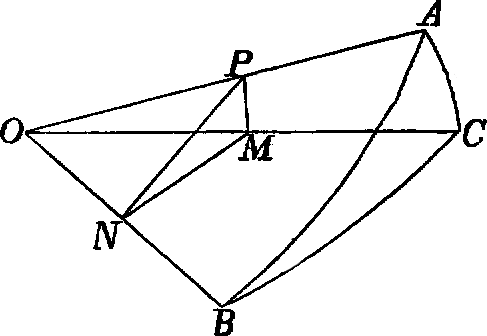
\includegraphics[width=5.0cm]{images/043fc}
\end{figure}

Let $ABC$ be a spherical triangle having a right angle at $C$;
let $O$ be the centre of the sphere. From any point $P$ in $OA$ draw
$PM$ perpendicular to $OC$, and from $M$ draw $MN$ perpendicular to
$OB$, and join $PN$. Then $PM$ is perpendicular to $MN$, because the
plane $AOC$ is perpendicular to the plane $BOC$; hence
\[
PN^2=PM^2+MN^2=OP^2-OM^2+OM^2-ON^2=OP^2-ON^2;
\]
therefore $PNO$ is a right angle. And
\begin{flalign*}
&&&\left.\begin{aligned}
&\rule{2em}{0pt}
\llap{$ \dfrac{ON}{OP}$}
\rlap{ $= \dfrac{ON}{OM} \centerdot\dfrac{OM}{OP}$, }
\rule[1em]{7em}{0pt}
\rule{6em}{0pt}
\llap{ that is, $\cos c$}
\rlap{ $=\cos a\cos b$,}
\rule[1em]{6em}{0pt}
\end{aligned}
\right.
&(1)&
\\[1ex]
&&&\left.\begin{aligned}
&\rule{2em}{0pt}
\llap{$ \dfrac{PM}{OP}$}
\rlap{ $= \dfrac{PM}{PN} \centerdot\dfrac{PN}{OP}$, }
\rule[1em]{7em}{0pt}
\rule{6em}{0pt}
\llap{ that is, $\sin b$}
\rlap{ $=\sin B\sin c$}
\rule[1em]{6em}{0pt}
\\
&\rule{15em}{0pt}
\llap{ Similarly,\qquad $\sin a$}
\rlap{ $=\sin A \sin c$}
\rule[1em]{5em}{0pt}
\end{aligned}
\right\},
&(2)&
\\[1ex]
&&&\left.\begin{aligned}
&\rule{2em}{0pt}
\llap{$ \dfrac{MN}{ON}$}
\rlap{ $= \dfrac{MN}{PN} \centerdot\dfrac{PN}{ON}$, }
\rule[1em]{7em}{0pt}
\rule{6em}{0pt}
\llap{ that is, $\tan a$}
\rlap{ $=\cos B\tan c$}
\rule[1em]{6em}{0pt}
\\
&\rule{15em}{0pt}
\llap{ Similarly,\qquad $\tan b$}
\rlap{ $= \cos A \tan c$}
\rule[1em]{5em}{0pt}
\end{aligned}
\right\},
&(3)&
\\[1ex]
&&&\left.\begin{aligned}
&\rule{2em}{0pt}
\llap{$ \dfrac{PM}{OM}$}
\rlap{ $= \dfrac{PM}{MN} \centerdot\dfrac{MN}{OM}$, }
\rule[1em]{7em}{0pt}
\rule{6em}{0pt}
\llap{ that is, $\tan b$}
\rlap{ $=\tan B\sin a$}
\rule[1em]{6em}{0pt}
\\
&\rule{15em}{0pt}
\llap{ Similarly,\qquad $\tan a$}
\rlap{ $= \tan A\sin b$}
\rule[1em]{5em}{0pt}
\end{aligned}
\right\}.
&(4)&
\end{flalign*}
%-----File: 044.png------------------------------------------------

Multiply together the two formul\ae\ (4); thus,
\[
  \tan A \tan B =
\dfrac{\tan a \tan b}{\sin a \sin b} =
\frac{1}{\cos a \cos b} =
\frac{1}{\cos c}\text{ by (1);}
\]
therefore \hfill$ \cos c = \cot A \cot B$.\hfill(5)
\\
Multiply crosswise the second formula in (2) and the first
in (3); thus \linebreak[4]$\sin a \cos B \tan c = \tan a \sin A \sin c$;
\begin{flalign*}
&\phantom{therefore}&&&\phantom{therefore}&\\[-\baselineskip]
&\rlap{therefore}&\multispan{2}{\hfil$\displaystyle
\cos B = \dfrac{\sin A \cos c}{\cos a} =
\sin A \cos b$ by (1).\hfil}\\[1ex]
&\begin{aligned}
&\text{Thus}\\
&\text{Similarly}
\end{aligned}&\multispan2{\hfil$\displaystyle
\left.\begin{aligned}
\cos B &= \sin A \cos b \\
\cos A &= \sin B \cos a
\end{aligned}\right\}$.\hfil}&\text{(6)}
\end{flalign*}

These six formul\ae\ comprise ten equations; and thus we can
solve every case of right-angled triangles. For every one of these
ten equations is a distinct combination involving three out of the
five quantities $a$, $b$, $c$, $A$, $B$; and out of five quantities only ten
combinations of three can be formed. Thus any two of the five
quantities being given and a third required, some one of the preceding
ten equations will serve to determine that third quantity.

\paragraph{63.} As we have stated, the above six formul\ae\ may be obtained
from those given in the preceding Chapter by supposing $C$ a
right angle. Thus (1) follows from Art.~39, (2) from Art.~41,
(3) from the fourth and fifth equations of Art.~44, (4) from the
first and second equations of Art.~44, (5) from the third equation
of Art.~47, (6) from the first and second equations of Art.~47.

Since the six formul\ae\ may be obtained from those given in
the preceding Chapter which have been proved to be universally
true, we do not stop to shew that the demonstration of Art.~62
may be applied to every case which can occur; the student may
for exercise investigate the modifications which will be necessary
when we suppose one or more of the quantities $a$, $b$, $c$, $A$, $B$ equal
to a right angle or greater than a right angle.
%-----File: 045.png------------------------------------------------

\paragraph{64.} Certain properties of right-angled triangles are deducible
from the formul\ae\ of Art.~62.

From (1) it follows that $\cos c$ has the same sign as the product
$\cos a\cos b$; hence either all the cosines are positive, or else only
one is positive. Therefore \textit{in a right-angled triangle either all the
three sides are less than quadrants, or else one side is less than a
quadrant and the other two sides are greater than quadrants.}

From (4) it follows that $\tan a$ has the same sign as $\tan A$.
Therefore $A$ and $a$ are either both greater than $\dfrac{\pi}{2}$, or both less
than $\dfrac{\pi}{2}$; this is expressed by saying that $A$ and $a$ are of the \textit{same
affection}. Similarly $B$ and $b$ are of the same affection.

\paragraph{65.} The formul\ae\ of Art.~62 are comprised in the following
enunciations, which the student will find it useful to remember;
the results are distinguished by the same numbers as have been
already applied to them in Art.~62; the side opposite the right
angle is called the \textit{hypotenuse:}
\begin{center}
\begin{tabular}{r@{\ }l@{}l}
  Cos hyp &= product of cosines of sides \dotfill&(1),\\[1ex]
  Cos hyp &= product of cotangents of angles \dotfill&(5),\\[1ex]
  Sine side &= sine of opposite angle $\times$ sine hyp \dotfill&(2),\\[1ex]
  Tan side &= tan hyp $\times$ cos included angle \dotfill&(3),\\[1ex]
  Tan side &= tan opposite angle $\times$ sine of other side \ldots\dotfill&(4),\\[1ex]
  Cos angle &= cos opposite side $\times$ sine of other angle \dotfill&(6).
\end{tabular}
\end{center}

\paragraph{66.} \textit{Napier's Rules}. The formul\ae\ of Art.~62 are comprised
in two rules, which are called, from their inventor, \textit{Napier's Rules
of Circular Parts}. Napier was also the inventor of Logarithms,
and the Rules of Circular Parts were first published by him in a
work entitled \textit{Mirifici Logarithmorum Canonis Descriptio}\dots\dots
Edinburgh, 1614. These rules we will now explain.
%-----File: 046.png------------------------------------------------

The right angle is left out of consideration; the two sides
which include the right angle, the complement of the hypotenuse,
and the complements of the other angles are called the \textit{circular
\begin{figure}[htp]
\centering
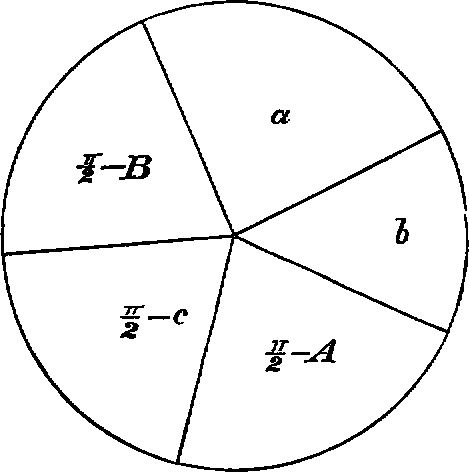
\includegraphics[width=5.0cm]{images/046fc}
\end{figure}
parts} of the triangle. Thus there are \textit{five} circular parts, namely,
$a$, $b$, $\dfrac{\pi}{2}-A$, $\dfrac{\pi}{2}-c$, $\dfrac{\pi}{2}-B$; and these are supposed to be ranged
round a circle in the order in which they naturally occur with
respect to the triangle.

Any one of the five parts may be selected and called the
\textit{middle part}, then the two parts next to it are called \textit{adjacent
parts}, and the remaining two parts are called \textit{opposite parts}. For
example, if $\dfrac{\pi}{2}-B$ is selected as the middle part, then the adjacent
parts are $a$ and $\dfrac{\pi}{2}-c$, and the opposite parts are $b$ and $\dfrac{\pi}{2}-A$.

Then Napier's Rules are the following:\\
sine of the middle part $=$ product of tangents of adjacent parts, \\
sine of the middle part $=$ product of cosines of opposite parts.

\paragraph{67.} Napier's Rules may be demonstrated by shewing that
they agree with the results already established. The following
table shews the required agreement: in the first column are given
the \textit{middle parts}, in the second column the results of Napier's
Rules, and in the third column the same results expressed as in
Art.~62, with the number for reference used in that Article.
%-----File: 047.png------------------------------------------------

\[
\begin{array}{@{}r@{\ } r@{\;}l@{ } r@{\;}l@{.}r}
   \dfrac{\pi}{2}-c
&  \sin\left(\dfrac{\pi}{2}-c\right)
&= \tan\left(\dfrac{\pi}{2}-A\right)
   \tan\left(\dfrac{\pi}{2}-B\right)
& \cos c &= \cot A \cot B \dotfill & (5),
\\[3ex]
&  \sin\left(\dfrac{\pi}{2}-c\right)
&= \cos a \cos b
&  \cos c &= \cos a \cos b \dotfill & (1),
\\[3ex]
   \dfrac{\pi}{2}-B
&         \sin\left(\dfrac{\pi}{2}-B\right)
&= \tan a \tan\left(\dfrac{\pi}{2}-c\right)
&  \cos B &= \tan a \cot c \dotfill & (3),
\\[3ex]
&         \sin\left(\dfrac{\pi}{2}-B\right)
&= \cos b \cos\left(\dfrac{\pi}{2}-A\right)
& \cos B &= \cos b \sin A \dotfill & (6),
\\[3ex]
a& \sin a
&= \tan b \tan \left(\dfrac{\pi}{2}-B\right)
&  \sin a &= \tan b \cot B \ldots\dotfill & (4),
\\[3ex]
&  \sin a
&= \cos\left(\dfrac{\pi}{2}-A\right)
   \cos\left(\dfrac{\pi}{2}-c\right)
&  \sin a &= \sin A \sin c \dotfill & (2),
\\[3ex]
b& \sin b
&= \tan\left(\dfrac{\pi}{2}-A\right) \tan a
&  \sin b &= \cot A\tan a \dotfill & (4),
\\[3ex]
&  \sin b
&= \cos\left(\dfrac{\pi}{2}-B\right)
   \cos\left(\dfrac{\pi}{2}-c\right)
&  \sin b &=\sin B \sin c \dotfill & (2),
\\[3ex]
   \dfrac{\pi}{2}-A
&        \sin\left(\dfrac{\pi}{2}-A\right)
&= \tan b \tan\left(\dfrac{\pi}{2}-c\right)
& \cos A &= \tan b\cot c \dotfill & (3),
\\[3ex]
&        \sin\left(\dfrac{\pi}{2}-A\right)
&= \cos a \cos\left(\dfrac{\pi}{2}-B\right)
& \cos A &= \cos a \sin B \dotfill & (6).
\end{array}
\]

The last four cases need not have been given, since it is obvious
that they are only repetitions of what had previously been given;
the seventh and eighth are repetitions of the fifth and sixth, and
the ninth and tenth are repetitions of the third and fourth.

\paragraph{68.} It has been sometimes stated that the method of the
preceding Article is the only one by which Napier's Rules can be
demonstrated; this statement, however, is inaccurate, since besides
this method Napier himself indicated another method of proof in
his \textit{Mirifici Logarithmorum Canonis Descriptio}, pp.\ 32, 35. This
we will now briefly explain.
%-----File: 048.png------------------------------------------------
\begin{figure}[htp]
\centering
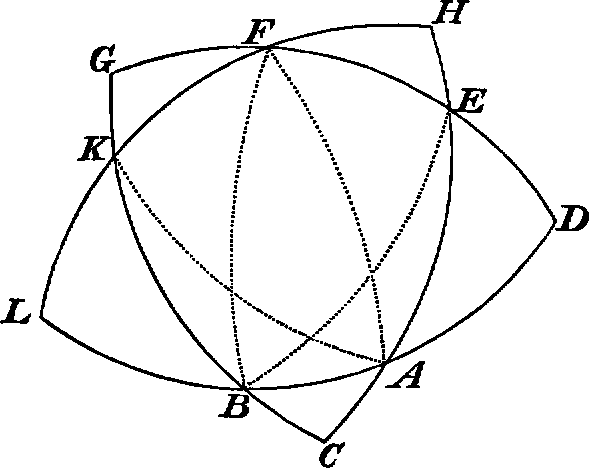
\includegraphics[width=5.0cm]{images/048fc}
\end{figure}

Let $ABC$ be a spherical triangle right-angled at $C$; with $B$
as pole describe a great circle $DEFG$, and with $A$ as pole describe
a great circle $HFKL$, and produce the sides of the original triangle
$ABC$ to meet these great circles. Then since $B$ is a pole of $DEFG$
the angles at $D$ and $G$ are right angles, and since $A$ is a pole of
$HFKL$ the angles at $H$ and $L$ are right angles. Hence the five
triangles $BAC$, $AED$, $EFH$, $FKG$, $KBL$ are all \textit{right-angled}; and
moreover it will be found on examination that, although the elements
of these triangles are different, yet \textit{their circular parts are
the same}. We will consider, for example, the triangle $AED$; the
angle $EAD$ is equal to the angle $BAC$, the side $AD$ is the complement
of $AB$; as the angles at $C$ and $G$ are right angles $E$ is a
pole of $GC$ (Art.~13), therefore $EA$ is the complement of $AC$; as
$B$ is a pole of $DE$ the angle $BED$ is a right angle, therefore the
angle $AED$ is the complement of the angle $BEC$, that is, the
angle $AED$ is the complement of the side $BC$ (Art.~12); and similarly
the side $DE$ is equal to the angle $DBE$, and is therefore the
complement of the angle $ABC$. Hence, if we denote the elements
of the triangle $ABC$ as usual by $a$, $b$, $c$, $A$, $B$, we have in the
triangle $AED$ the hypotenuse equal to $\dfrac{\pi}{2} - b$, the angles equal to
$A$ and $\dfrac{\pi}{2} - a$, and the sides respectively opposite these angles equal
to $\dfrac{\pi}{2} - B$ and $\dfrac{\pi}{2} - c$. The \textit{circular parts} of $AED$ are therefore the
%-----File: 049.png------------------------------------------------
same as those of $ABC$. Similarly the remaining three of the five
right-angled triangles may be shewn to have the same circular
parts as the triangle $ABC$ has.

Now take \textit{two} of the theorems in Art.~65, for example (1) and
(3); then the truth of the \textit{ten} cases comprised in Napier's Rules
will be found to follow from applying the two theorems in succession
to the five triangles formed in the preceding figure. Thus
this method of considering Napier's Rules regards each Rule, not
as the statement of dissimilar properties of one triangle, but as the
statement of similar properties of five allied triangles.

\paragraph{69.} In Napier's work a figure is given of which that in the
preceding Article is a copy, except that different letters are used;
Napier briefly intimates that the truth of the Rules can be easily
seen by means of this figure, as well as by the method of induction
from consideration of all the cases which can occur. The late
T.~S. Davies, in his edition of Dr Hutton's \textit{Course of Mathematics},
drew attention to Napier's own views and expanded the demonstration
by a systematic examination of the figure of the preceding
Article.

It is however easy to evade the necessity of examining the
whole figure; all that is wanted is to observe the connexion
between the triangle $AED$ and the triangle $BAC$. For let $a_1$, $a_2$,
$a_3$, $a_4$, $a_5$ represent the elements of the triangle $BAC$ taken in
order, beginning with the hypotenuse and omitting the right
angle; then the elements of the triangle $AED$ taken in order,
beginning with the hypotenuse and omitting the right angle, are
$\dfrac{\pi}{2} - a_3$, $\dfrac{\pi}{2} - a_4$, $\dfrac{\pi}{2} - a_5$,
$\dfrac{\pi}{2} - a_1$, and $a_2$. If, therefore, to characterise
the former we introduce a new set of quantities $p_1$, $p_2$, $p_3$, $p_4$, $p_5$,
such that $a_1 + p_1 = a_2 + p_2 = a_5 + p_5 = \dfrac{\pi}{2}$, and that $p_3 = a_3$ and $p_4 = a_4$,
then the original triangle being characterised by $p_1$, $p_2$, $p_3$, $p_4$, $p_5$,
the second triangle will be similarly characterised by $p_3$, $p_4$, $p_5$,
$p_1$, $p_2$. As the second triangle can give rise to a third in like
manner, and so on, we see that every right-angled triangle is one
%-----File: 050.png------------------------------------------------
of a system of five such triangles which are all characterised by
the quantities $p_1$, $p_2$, $p_3$, $p_4$, $p_5$, always taken in order, each
quantity in its turn standing first.

The late R.~L.\ Ellis pointed out this connexion between the
five triangles, and thus gave the true significance of Napier's
Rules. The memoir containing Mr Ellis's investigations, which
was unpublished when the first edition of the present work appeared,
will be found in pages 328\ldots335 of \textit{The Mathematical and
other writings of Robert Leslie Ellis}\dots Cambridge, 1863.

Napier's own method of considering his Rules was neglected
by writers on the subject until the late T.~S.\ Davies drew attention
to it. Hence, as we have already remarked in Art.\ 68, an
erroneous statement was made respecting the Rules. For instance,
Woodhouse says, in his \textit{Trigonometry}: ``There is no separate
and independent proof of these rules;\ldots.'' Airy says, in the
treatise on Trigonometry in the \textit{Encyclop\ae dia Metropolitana}:
``These rules are proved to be true only by showing that they comprehend
all the equations which we have just found.''

\paragraph{70.} Opinions have differed with respect to the \textit{utility} of
Napier's Rules in practice. Thus Woodhouse says, ``In the whole
compass of mathematical science there cannot be found, perhaps,
rules which more completely attain that which is the proper
object of rules, namely, facility and brevity of computation.''
(\textit{Trigonometry}, chap.\ \textsc{x}.) On the other hand may be set the following
sentence from Airy's Trigonometry (\textit{Encyclop\ae dia Metropolitana}):
``In the opinion of Delambre (and no one was better
qualified by experience to give an opinion) these theorems are best
recollected by the practical calculator in their unconnected form.''
See Delambre's \textit{Astronomie}, vol.~\textsc{i}.\ p.~205. Professor De Morgan
strongly objects to Napier's Rules, and says (\textit{Spherical Trigonometry},
Art.~17): ``There are certain mnemonical formul\ae\ called
\textit{Napier's Rules of Circular Parts}, which are generally explained.
We do not give them, because we are convinced that they only
create confusion instead of assisting the memory.''
%-----File: 051.png------------------------------------------------

\paragraph{71.} We shall now proceed to apply the formul\ae\ of Art.\ 62
to the solution of right-angled triangles. We shall assume that
the given quantities are subject to the limitations which are stated
in Arts.\ 22 and 23, that is, a given side must be less than the
semicircumference of a great circle, and a given angle less than
two right angles. There will be six cases to consider.

\paragraph{72.} \textit{Having given the hypotenuse $\mathrm{c}$ and an angle $\mathrm{A}$.}

Here we have from (3), (5) and (2) of Art.\ 62,
\[
\tan b = \tan c \cos A,\quad \cot B = \cos c \tan A,\quad \sin a = \sin c \sin A.
\]

Thus $b$ and $B$ are determined immediately without ambiguity;
and as $a$ must be of the same affection as $A$ (Art.\ 64), $a$ also is
determined without ambiguity.

It is obvious from the formul\ae\ of solution, that in this case
the triangle is always possible.

If $c$ and $A$ are both right angles, $a$ is a right angle, and $b$ and
$B$ are indeterminate.

\paragraph{73.} \textit{Having given a side $\mathrm{b}$ and the adjacent angle $\mathrm{A}$.}

Here we have from (3), (4) and (6) of Art.\ 62,
\[
\tan c=\dfrac{\tan b}{\cos A},\quad \tan a = \tan A \sin b,\quad \cos B = \cos b \sin A.
\]

Here $c$, $a$, $B$ are determined without ambiguity, and the triangle
is always possible.

\paragraph{74.} \textit{Having given the two sides $\mathrm{a}$ and $\mathrm{b}$.}

Here we have from (1) and (4) of Art.\ 62,
\[
\cos c = \cos a \cos b,\quad \cot A = \cot a \sin b,\quad \cot B = \cot b \sin a.
\]

Here $c$, $A$, $B$ are determined without ambiguity, and the triangle
is always possible.

\paragraph{75.} \textit{Having given the hypotenuse $\mathrm{c}$ and a side $\mathrm{a}$.}

Here we have from (1), (3) and (2) of Art.\ 62,
\[
\cos b=\dfrac{\cos c}{\cos a},\quad \cos B=\dfrac{\tan a}{\tan c},\quad \sin A=\dfrac{\sin a}{\sin c}.
\]
%-----File: 052.png------------------------------------------------

Here $b$, $B$, $A$ are determined without ambiguity, since $A$ must
be of the same affection as $a$. It will be seen from these formul\ae\
that there are limitations of the data in order to insure a possible
triangle; in fact, $c$ must lie between $a$ and $\pi - a$ in order that the
values found for $\cos b$, $\cos B$, and $\sin A$ may be numerically not
greater than unity.

If $c$ and $a$ are right angles, $A$ is a right angle, and $b$ and $B$ are
indeterminate.

\paragraph{76.} \textit{Having given the two angles $\mathrm{A}$ and $\mathrm{B}$.}

Here we have from (5) and (6) of Art.\ 62,
\[
\cos c = \cot A \cot B, \qquad
\cos a = \frac{\cos A}{\sin B}, \qquad
\cos b = \frac{\cos B}{\sin A}.
\]

Here $c$, $a$, $b$ are determined without ambiguity. There are
limitations of the data in order to insure a possible triangle. First
suppose $A$ less than $\dfrac{\pi}{2}$, then $B$ must lie between $\dfrac{\pi}{2} - A$ and $\dfrac{\pi}{2} + A$;
next suppose $A$ greater than $\dfrac{\pi}{2}$, then $B$ must lie between
$\dfrac{\pi}{2} - (\pi - A)$ and
$\dfrac{\pi}{2} + (\pi - A)$, that is, between
$A - \dfrac{\pi}{2}$ and $\dfrac{3\pi}{2} - A$.

\paragraph{77.} \textit{Having given a side $\mathrm a$ and the opposite angle $\mathrm A$.}

Here we have from (2), (4) and (6) of Art.\ 62,
\[
\sin c = \dfrac{\sin a}{\sin A}, \qquad
\sin b = \tan a\, \cot A, \qquad
\sin B = \dfrac{\cos A}{\cos a}.
\]

Here there is an ambiguity, as the parts are determined from
their sines. If $\sin a$ be less than $\sin A$, there are two values
admissible for $c$; corresponding to each of these there will be
\textit{in general} only one admissible value of $b$, since we must have
$\cos c = \cos a\, \cos b$, and only one admissible value of $B$, since we
must have $\cos c = \cot A \cot B$. Thus if one triangle exists with the
given parts, there will be \textit{in general} two, and only two, triangles
with the given parts. We say \textit{in general} in the preceding sentences,
because if $a = A$ there will be only \textit{one} triangle, unless $a$
%-----File: 053.png------------------------------------------------
and $A$ are each right angles, and then $b$ and $B$ become indeterminate.

It is easy to see from a figure that the ambiguity must occur
in general.
\begin{figure}[htp]
\centering
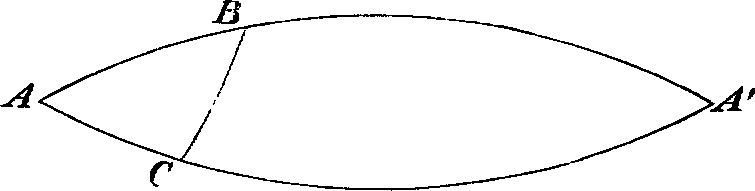
\includegraphics[width=5.0cm]{images/053fc}
\end{figure}

For, suppose $BAC$ to be a triangle which satisfies the given
conditions; produce $AB$ and $AC$ to meet again at $A'$; then the
triangle $A'BC$ also satisfies the given conditions, for it has a right
angle at $C$, $BC$ the given side, and $A' = A$ the given angle.

If $a = A$, then the formul\ae\ of solution shew that $c$, $b$, and $B$
are right angles; in this case $A$ is the pole of $BC$, and the triangle
$A'BC$ is symmetrically equal to the triangle $ABC$ (Art.\ 57).

If $a$ and $A$ are both right angles, $B$ is the pole of $AC$; $B$ and $b$
are then equal, but may have any value whatever.

There are limitations of the data in order to insure a possible
triangle. $A$ and $a$ must have the same affection by Art.\ 64; hence
the formul\ae\ of solution shew that $a$ must be less than $A$ if both
are acute, and greater than $A$ if both are obtuse.

\section*{\centering\normalsize EXAMPLES.}

If $ABC$ be a triangle in which the angle $C$ is a right angle,
prove the following relations contained in Examples 1 to 5.
\medskip

1. $\operatorname{Sin}^2\dfrac{c}{2} =
                      \sin^2 \dfrac{a}{2}\, \cos^2 \dfrac{b}{2} +
                      \cos^2 \dfrac{a}{2}\, \sin^2 \dfrac{b}{2}$.
\medskip

2. $\operatorname{Tan}\tfrac{1}{2}(c + a)\,
                      \tan \tfrac{1}{2}(c - a) =
                      \tan^2 \dfrac{b}{2}$.
\medskip

3. $\operatorname{Sin}(c - b) = \tan^2 \dfrac{A}{2}\,\sin(c + b)$.
%-----File: 054.png------------------------------------------------
\medskip

4. $\operatorname{Sin} a\, \tan \tfrac{1}{2}A
                     - \sin b\, \tan \tfrac{1}{2}B = \sin (a - b)$.

\begin{flalign*}
\rlap{\indent 5.} && \operatorname{Sin} (c - a)
&= \sin b\, \cos a\, \tan \tfrac{1}{2}B, &&\\
&& \operatorname{Sin} (c - a)
&= \tan b\, \cos c\, \tan \tfrac{1}{2}B. &&
\end{flalign*}

6. If $ABC$ be a spherical triangle, right-angled at $C$, and
$\cos A = \cos^2 a$, shew that if $A$ be not a right angle $b + c = \tfrac{1}{2}\pi$ or
$\dfrac{3}{2}\pi$, according as $b$ and $c$ are both less or both greater than $\dfrac{\pi}{2}$.
\medskip

7. If $\alpha$, $\beta$ be the arcs drawn from the right angle respectively
perpendicular to and bisecting the hypotenuse $c$, shew that
\[
\sin^2 \dfrac{c}{2}\,(1 + \sin^2\alpha) + \sin^2\beta.
\]

8. In a triangle, if $C$ be a right angle and $D$ the middle point
of $AB$, shew that
\[
4\cos^2\dfrac{c}{2}\, \sin^2 CD = \sin^2 a + \sin^2 b.
\]

9. In a right-angled triangle, if $\delta$ be the length of the arc
drawn from $C$ perpendicular to the hypotenuse $AB$, shew that
\[
\cot\delta = \surd{(\cot^2a + \cot^2b)}.
\]

10. $OAA_1$ is a spherical triangle right-angled at $A_1$ and acute-angled
at $A$; the arc $A_1A_2$ of a great circle is drawn perpendicular
to $OA$, then $A_2A_3$ is drawn perpendicular to $OA_1$, and so on: shew
that $A_nA_{n+1}$ vanishes when $n$ becomes infinite; and find the value
of $\cos AA_1 \cos A_1A_2 \cos A_2A_3\ldots\ldots$ to infinity.
\medskip

11. $ABC$ is a right-angled spherical triangle, $A$ not being the
right angle: shew that if $A = a$, then $c$ and $b$ are quadrants.
\medskip

12. If $\delta$ be the length of the arc drawn from $C$ perpendicular
to $AB$ in \textit{any} triangle, shew that
\[
\cos\delta = \operatorname{cosec} c\, (\cos^2 a + \cos^2 b - 2 \cos a\, \cos b\, \cos c)^{\tfrac{1}{2}}.
\]

13. $ABC$ is a great circle of a sphere; $AA'$, $BB'$, $CC'$, are arcs
of great circles drawn at right angles to $ABC$ and reckoned positive
%-----File: 055.png------------------------------------------------
when they lie on the same side of it: shew that the condition
of $A'$, $B'$, $C'$ lying in a great circle is
\[
\tan AA'\, \sin BC + \tan BB'\, \sin CA + \tan CC'\, \sin AB = 0.
\]

14. Perpendiculars are drawn from the angles $A$, $B$, $C$ of any
triangle meeting the opposite sides at $D$, $E$, $F$ respectively: shew
that
\[
\tan BD\, \tan CE\, \tan AF = \tan DC\, \tan EA\, \tan FB.
\]

15. $Ox$, $Oy$ are two great circles of a sphere at right angles to
each other, $P$ is any point in $AB$ another great circle. $OC = p$ is
the arc perpendicular to $AB$ from $O$, making the angle $COx = a$
with $Ox$. $PM$, $PN$ are arcs perpendicular to $Ox$, $Oy$ respectively:
shew that if $OM = x$ and $ON = y$,
\[
\cos a\, \tan x + \sin a\, \tan y = \tan p.
\]

16. The position of a point on a sphere, with reference to two
great circles at right angles to each other as axes, is determined
by the portions $\theta$, $\phi$ of these circles cut off by great circles through
the point, and through two points on the axes, each $\dfrac{\pi}{2}$ from their
point of intersection: shew that if the three points ($\theta$, $\phi$), ($\theta'$, $\phi'$),
($\theta''$, $\phi''$) lie on the same great circle
\begin{gather*}
  \tan \phi\, (\tan \theta' - \tan \theta'')
+ \tan \phi'\, (\tan \theta'' - \tan \theta)\\
+ \tan \phi''\, (\tan \theta - \tan \theta') = 0.
\end{gather*}

17. If a point on a sphere be referred to two great circles at
right angles to each other as axes, by means of the portions of
these axes cut off by great circles drawn through the point and
two points on the axes each $90^\circ$ from their intersection, shew that
the equation to a great circle is
\[
\tan \theta\, \cot \alpha + \tan \phi\, \cot \beta = 1.
\]

18. In a spherical triangle, if $A = \dfrac{\pi}{5}$, $B = \dfrac{\pi}{3}$, and, $C = \dfrac{\pi}{2}$, shew that\, $a + b + c = \dfrac{\pi}{2}$.
%-----File: 056.png------------------------------------------------

\chapter[Solution of Oblique-Angled Triangles.]{SOLUTION OF OBLIQUE-ANGLED TRIANGLES.}

\paragraph{78.} The solution of oblique-angled triangles may be made in
some cases to depend immediately on the solution of right-angled
triangles; we will indicate these cases before considering the subject
generally.

(1) Suppose a triangle to have one of its given sides equal to
a \textit{quadrant}. In this case the polar triangle has its corresponding
angle a right angle; the polar triangle can therefore be solved by
the rules of the preceding Chapter, and thus the elements of the
primitive triangle become known.

(2) Suppose among the given elements of a triangle there are
two \textit{equal sides} or two \textit{equal angles}. By drawing an arc from the
vertex to the middle point of the base, the triangle is divided into
two equal \textit{right-angled} triangles; by the solution of one of these
right-angled triangles the required elements can be found.

(3) Suppose among the given elements of a triangle there
are two sides, one of which is the supplement of the other, or two
angles, one of which is the supplement of the other. Suppose, for
example, that $b + c = \pi$, or else that $B + C = \pi$; produce $BA$ and
$BC$ to meet at $B'$ (see the first figure to Art.\ 38); then the triangle
$B'AC$ has two equal sides given, or else two equal angles given;
and by the preceding case the solution of it can be made to depend
on the solution of a right-angled triangle.

\paragraph{79.} We now proceed to the solution of oblique-angled triangles
in general. There will be six cases to consider.

\paragraph{80.} \textit{Having given the three sides.}

Here we have $\cos A = \dfrac{\cos a - \cos b \cos c}{\sin b \sin c}$, and similar formul\ae\
for $\cos B$ and $\cos C$. Or if we wish to use formul\ae\ suited to logarithms,
%-----File: 057.png------------------------------------------------
we may take the formula for the sine, cosine, or tangent of
half an angle given in Art.~45. In selecting a formula, attention
should be paid to the remarks in \textit{Plane Trigonometry}, Chap.~XII.
towards the end.

\paragraph{81.} \textit{Having given the three angles.}

Here we have $\cos a = \dfrac{\cos A + \cos B \cos C}{\sin B \sin C}$, and similar formul\ae\
for $\cos b$ and $\cos c$. Or if we wish to use formul\ae\ suited to logarithms,
we may take the formula for the sine, cosine, or tangent of
half a side given in Art.~49.

There is no ambiguity in the two preceding cases; the triangles
however may be impossible with the given elements.

\paragraph{82.} \textit{Having given two sides and the included angle} ($a$, $C$, $b$).

By Napier's analogies
\begin{align*}
&\tan \tfrac{1}{2}(A + B) = \dfrac{\cos\tfrac{1}{2}(a - b)}{\cos\tfrac{1}{2}(a + b)}\cot\tfrac{1}{2}C,\\[1ex]
&\tan \tfrac{1}{2}(A - B) = \dfrac{\sin\tfrac{1}{2}(a - b)}{\sin\tfrac{1}{2}(a + b)}\cot\tfrac{1}{2}C;
\end{align*}
these determine $\tfrac{1}{2}(A + B)$ and $\tfrac{1}{2}(A - B)$, and thence $A$ and $B$.

Then $c$ may be found from the formula $\sin c = \dfrac{\sin a\, \sin C}{\sin A}$; in
this case, since $c$ is found from its sine, it may be uncertain which
of two values is to be given to it; the point may be sometimes
settled by observing that the greater side of a triangle is opposite
to the greater angle. Or we may determine $c$ from equation (1) of
Art.~54, which is free from ambiguity.

Or we may determine $c$, without previously determining $A$ and
$B$, from the formula $\cos c = \cos a\, \cos b + \sin a\, \sin b\, \cos C$; this is
free from ambiguity. This formula may be adapted to logarithms
thus:
\[
\cos c = \cos b\, (\cos a + \sin a \tan b \cos C);
\]
%-----File: 058.png------------------------------------------------
assume $\tan \theta = \tan b\, \cos C$; then
\[
\cos c = \cos b\, (\cos a + \sin a\, \tan \theta) = \dfrac{\cos b\, \cos (a - \theta)}{\cos \theta};
\]
this is adapted to logarithms.
\begin{figure}[htp]
\centering
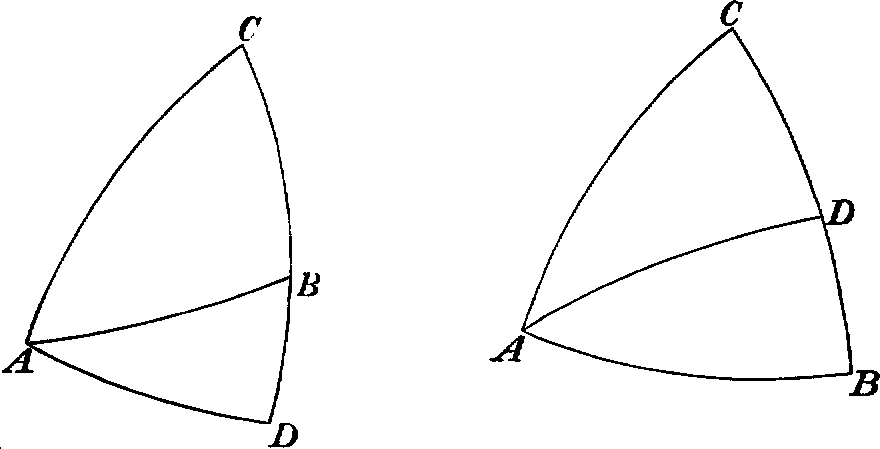
\includegraphics[width=5.0cm]{images/058fc}
\end{figure}

Or we may treat this case conveniently by resolving the triangle
into the sum or difference of two right-angled triangles.
From $A$ draw the arc $AD$ perpendicular to $CB$ or $CB$ produced;
then, by Art.\ 62, $\tan CD = \tan b \cos C$, and this determines $CD$,
and then $DB$ is known. Again, by Art.\ 62,
\[
\cos c = \cos AD \cos DB = \cos DB \dfrac{\cos b}{\cos CD};
\]
this finds $c$. It is obvious that $CD$ is what was denoted by $\theta$ in
the former part of the Article.

By Art.\ 62,
\begin{gather*}
  \tan AD = \tan C \sin CD,\text{ and }\tan AD = \tan ABD \sin DB; \\
  \text{thus } \tan ABD \sin DB = \tan C \sin \theta,
\end{gather*}
where $DB = a - \theta$ or $\theta - a$, according as $D$ is on $CB$ or $CB$ produced,
and $ABD$ is either $B$ or the supplement of $B$; this formula
enables us to find $B$ independently of $A$.

Thus, in the present case, there is no real ambiguity, and the
triangle is always possible.
%-----File: 059.png------------------------------------------------

\paragraph{83.} \textit{Having given two angles and the included side $\mathrm{(A, c, B)}$.}

By Napier's analogies,
\begin{align*}
   \tan \tfrac{1}{2} (a + b)
&= \dfrac{\cos \tfrac{1}{2} (A - B)}{\cos \tfrac{1}{2} (A + B)} \tan \tfrac{1}{2} c, \\[1ex]
   \tan \tfrac{1}{2} (a - b)
&= \dfrac{\sin \tfrac{1}{2} (A - B)}{\sin \tfrac{1}{2} (A + B)} \tan \tfrac{1}{2} c;
\end{align*}
these determine $\tfrac{1}{2} (a + b)$ and $\tfrac{1}{2} (a - b)$, and thence $a$ and $b$.

Then $C$ may be found from the formula $\sin C = \dfrac{\sin A \sin c}{\sin a}$; in
this case, since $C$ is found from its sine, it may be uncertain which
of two values is to be given to it; the point may be sometimes
settled by observing that the greater angle of a triangle is opposite
to the greater side. Or we may determine $C$ from equation (3) of
Art.\ 54, which is free from ambiguity.

Or we may determine $C$ without previously determining $a$ and
$b$ from the formula $\cos C = -\cos A \cos B + \sin A \sin B \cos c$. This
formula may be adapted to logarithms, thus:
\[
\cos C = \cos B (-\cos A + \sin A\, \tan B\, \cos c);
\]
assume $\cot \phi = \tan B\, \cos c$; then
\[
\cos C = \cos B (-\cos A + \cot \phi \sin A) = \dfrac{\cos B \sin (A-\phi)}{\sin \phi}\,;
\]
this is adapted to logarithms.

Or we may treat this case conveniently by resolving the triangle
into the sum or difference of two right-angled triangles.
From $A$ draw the arc $AD$ perpendicular to $CB$ (see the right-hand
figure of Art.\ 82); then, by Art.\ 62, $\cos c = \cot B \cot DAB$,
and this determines $DAB$, and then $CAD$ is known. Again,
by Art.\ 62,
\[
\cos AD \sin CAD = \cos C,\text{ and }\cos AD \sin BAD = \cos B;
\]
therefore $\dfrac{\cos C}{\sin CAD}
= \dfrac{\cos B}{\sin BAD}$; this finds $C$.
\\[1ex]
It is obvious that $DAB$ is what was denoted by $\phi$ in the former
part of the Article.
%-----File: 060.png------------------------------------------------

By Art.\ 62,
\[
  \tan AD = \tan AC \cos CAD,\text{ and }
  \tan AD = \tan AB \cos BAD;
\]
thus \hfill$\tan b \cos CAD = \tan c \cos \phi$,\hfill\phantom{thus}\\[1ex]
where $CAD = A - \phi$; this formula enables us to find $b$ independently
of $a$.

Similarly we may proceed when the perpendicular $AD$ falls on
$CB$ \textit{produced}; (see the left-hand figure of Art.~82).

Thus, in the present case, there is no real ambiguity; moreover
the triangle is always possible.

\paragraph{84.} \textit{Having given two sides and the angle opposite one of them
$(\mathrm a$, $\mathrm b$, $\mathrm A)$.}

The angle $B$ may be found from the formula
\[
  \sin B = \frac{\sin b}{\sin a} \sin A;
\]
and then $C$ and $c$ may be found from Napier's analogies,
\begin{align*}
  \tan \tfrac{1}{2} C
&= \dfrac{\cos \tfrac{1}{2} (a - b)}
        {\cos \tfrac{1}{2} (a + b)} \cot \tfrac{1}{2} (A + B),
\\[1ex]
  \tan \tfrac{1}{2} c
&= \dfrac{\cos \tfrac{1}{2} (A + B)}
        {\cos \tfrac{1}{2} (A - B)} \tan \tfrac{1}{2} (a + b).
\end{align*}
In this case, since $B$ is found from its sine, there will sometimes
be two solutions; and sometimes there will be no solution at all,
namely, when the value found for $\sin B$ is greater than unity. We
will presently return to this point. (See Art.~86.)

We may also determine $C$ and $c$ independently of $B$ by formul\ae\
adapted to logarithms. For, by Art.~44,
\[
  \cot a\, \sin b
= \cos b\, \cos C + \sin C\, \cot A
= \cos b\, (\cos C + \dfrac{\cot A}{\cos b}\, \sin C);
\]
assume $\tan \phi = \dfrac{\cot A}{\cos b}$; thus
\[
  \cot a\, \sin b
= \cos b (\cos C + \tan \phi\, \sin C)
= \dfrac{\cos b\, \cos (C - \phi)}{\cos \phi};
\]
therefore \hfill $
  \cos (C - \phi) = \cos \phi \cot a \tan b$; \hfill\phantom{therefore}\\
%-----File: 061.png------------------------------------------------
from this equation $C - \phi$ is to be found, and then $C$. The ambiguity
still exists; for if the last equation leads to $C - \phi = a$, it
will be satisfied also by $\phi - C = a$; so that we have two admissible
values for $C$, if $\phi + a$ is less than $\pi$, and $\phi - a$ is positive.

And
\[
\cos a = \cos b \cos c + \sin b \sin c \cos A = \cos b (\cos c + \sin c \tan b \cos A);
\]
assume $\tan\theta = \tan b \cos A$; thus
\[
\cos a = \cos b (\cos c + \sin c \tan \theta) = \dfrac{\cos b\cos(c -\theta)}{\cos\theta};
\]
therefore \hfill$
\cos(c - \theta) = \dfrac{\cos a \cos\theta}{\cos b};
$\hfill\phantom{therefore}\\[2ex]
from this equation $c - \theta$ is to be found, and then $c$; and there may
be an ambiguity as before.

Or we may treat this case conveniently by resolving the triangle
into the sum or difference of two right-angled triangles.
\begin{figure}[htp]
\centering
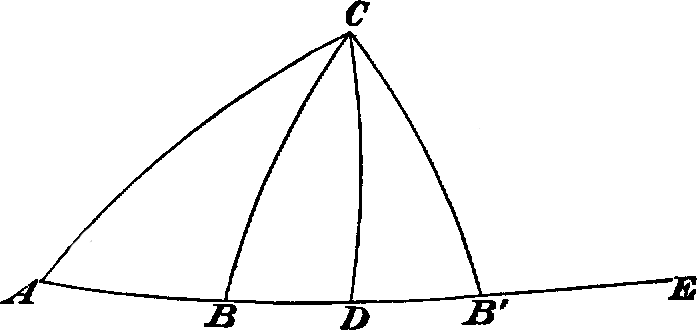
\includegraphics[width=5.0cm]{images/061fc}
\end{figure}

Let $CA = b$, and let $CAE = \text{the given angle }A$; from $C$ draw
$CD$ perpendicular to $AE$, and let $CB$ and $CB' = a$; thus the figure
shews that there may be two triangles which have the given elements.
Then, by Art.~62, $\cos b = \cot A \cot ACD$; this finds $ACD$.
Again, by Art.~62,
\begin{align*}
&\tan CD = \tan AC \cos ACD, \\
&\text{and } \tan CD = \tan CB \cos BCD, \text{ or }
                       \tan CB' \cos B'CD,
\end{align*}
therefore $\tan AC \cos ACD = \tan CB \cos BCD$, or $\tan CB' \cos B'CD$;
this finds $BCD$ or $B'CD$.

It is obvious that $ACD$ is what was denoted by $\phi$ in the former
part of the Article.
%-----File: 062.png------------------------------------------------

\begin{flalign*}
\text{\indent Also, by Art.\ 62, }
  \tan AD &= \tan AC cos A; \text{ this finds $AD$. Then }&&\\
  \cos AC &= \cos CD \cos AD, \\
  \cos CB &= \cos CD \cos BD, \\
  \text{ or }\cos CB' &= \cos CD \cos B'D;
\end{flalign*}
therefore \hfill$\displaystyle
  \dfrac{\cos AC}{\cos AD}
= \dfrac{\cos CB}{\cos BD} \text{ or }
  \dfrac{\cos CB'}{\cos B'D}$; \hfill\phantom{therefore}\\[1ex]
this finds $BD$ or $B'D$.

It is obvious that $AD$ is what was denoted by $\theta$ in the former
part of the Article.

\paragraph{85.} \textit{Having given two angles and the side opposite one of them
$(\mathrm A$, $\mathrm B$, $\mathrm a)$.}

This case is analogous to that immediately preceding, and
gives rise to the same ambiguities. The side $b$ may be found from
the formula
\[
  \sin b=\dfrac{\sin B \sin a}{\sin A};
\]
and then $C$ and $c$ may be found from Napier's analogies,
\begin{align*}
  \tan \tfrac{1}{2}C
&= \dfrac{\cos\tfrac{1}{2}(a-b)}
        {\cos\tfrac{1}{2}(a+b)} \cot\tfrac{1}{2}(A+B),
\\[1ex]
  \tan \tfrac{1}{2}c
&= \dfrac{\cos\tfrac{1}{2}(A+B)}
        {\cos\tfrac{1}{2}(A-B)} \tan\tfrac{1}{2}(a+b),
\end{align*}

We may also determine $C$ and $c$ independently of $b$ by formul\ae\
adapted to logarithms. For
\begin{multline*}
  \cos A= -\cos B\cos C + \sin B\sin C\cos a \\
= \cos B (-\cos C + \tan B\sin C \cos a),
\end{multline*}
assume $\cot \phi=\tan B \cos a;$ thus
\[
  \cos A = \cos B(-\cos C + \sin C \cot \phi)
= \dfrac{\cos B\sin(C - \phi)}{\sin \phi};
\]
$\rlap{therefore }\hfill\displaystyle
  \sin(C - \phi)=\dfrac{\cos A \sin \phi}{\cos B}; \hfill$ \\[1ex]
%-----File: 063.png------------------------------------------------
from this equation $C-\phi$ is to be found and then $C$. Since $C-\phi$
is found from its sine there may be an ambiguity. Again, by
Art.~44,
\[
\cot A \sin B = \cot a \sin c - \cos c \cos B =
\cos B \left(- \cos c + \dfrac{\cot a \sin c}{\cos B}\right),
\]
$\text{assume } \cot \theta = \dfrac{\cot a}{\cos B}; \text{ then}$
\[
\cot A \sin B = \cos B (- \cos c + \sin c \cot \theta) =
\frac{\cos B \sin (c - \theta)}{\sin \theta};
\]
$\rlap{therefore }\hfill
\sin (c - \theta) = \cot A \tan B \sin \theta;
\hfill$\\[1ex]
from this equation $c - \theta$ is to be found, and then $c$. Since $c - \theta$ is
found from its sine there may be an ambiguity. As before, it may
be shewn that these results agree with those obtained by resolving
the triangle into two right-angled triangles; for if in the triangle
$ACB'$ the arc $CD$ be drawn perpendicular to $AB'$, then $B'CD$
will $=\phi$, and $B'D = \theta$.

\paragraph{86.} We now return to the consideration of the ambiguity
which may occur in the case of Art.\ 84, when two sides are given
and the angle opposite one of them. The discussion is somewhat
tedious from its length, but presents no difficulty.

Before considering the problem generally, we will take the
particular case in which $a = b$; then $A$ must $= B$. The first and
third of Napier's analogies give
\[
\cot \tfrac{1}{2}C = \tan A \cos a,\qquad \tan \tfrac{1}{2}c = \tan a \cos A;
\]
now $\cot \tfrac{1}{2}C$ and $\tan \tfrac{1}{2}c$ must both be \textit{positive}, so that $A$ and $a$ must
be of the same affection. Hence, when $a = b$, there will be no
solution at all, unless $A$ and $a$ are of the same affection, and then
there will be only one solution; except when $A$ and $a$ are both
right angles, and then $\cot \tfrac{1}{2}C$ and $\tan\tfrac{1}{2}c$ are indeterminate, and
there is an infinite number of solutions.

We now proceed to the general discussion.

If $\sin b \sin A$ be greater than $\sin a$, there is no triangle which
satisfies the given conditions; if $\sin b \sin A$ is \textit{not} greater than
%-----File: 064.png------------------------------------------------
$\sin a$, the equation $\sin B = \dfrac{\sin b \sin A}{\sin a}$ furnishes two values of $B$,
which we will denote by $\beta$ and $\beta'$, so that $\beta' = \pi - \beta$; we will suppose
that $\beta$ is the one which is not greater than the other.

Now, in order that these values of $B$ may be admissible, it is
necessary and sufficient that the values of $\cot\frac{1}{2}C$ and of $\tan\frac{1}{2}c$
should both be positive, that is, $A-B$ and $a-b$ must have the
same sign by the second and fourth of Napier's analogies. We
have therefore to compare the sign of $A-\beta$ and the sign of $A-\beta'$
with that of $a-b$.

We will suppose that $A$ is less than a right angle, and separate
the corresponding discussion into three cases.\medskip

I\@. Let $b$ be less than $\dfrac{\pi}{2}$.

(1) Let $a$ be less than $b$; the formula $\sin B = \dfrac{\sin b}{\sin a}\sin A$ make
$\beta$ greater than $A$, and \textit{\`a fortiori} $\beta'$ greater than $A$. Hence there
are two solutions.

(2) Let $a$ be equal to $b$; then there is one solution, as previously
shewn.

(3) Let $a$ be greater than $b$; we may have then $a + b$ less than
$\pi$ or equal to $\pi$ or greater than $\pi$. If $a + b$ is less than $\pi$, then
$\sin a$ is greater than $\sin b$; thus $\beta$ is less than $A$ and therefore
admissible, and $\beta'$ is greater than $A$ and inadmissible. Hence there
is one solution. If $a + b$ is equal to $\pi$, then $\beta$ is equal to $A$, and
$\beta'$ greater than $A$, and both are inadmissible. Hence there is no
solution. If $a+b$ is greater than $\pi$, then $\sin a$ is less than $\sin b$,
and $\beta$ and $\beta'$ are both greater than $A$, and both inadmissible.
Hence there is no solution.\medskip

II\@. Let $b$ be equal to $\dfrac{\pi}{2}$.

(1) Let $a$ be less than $b$; then $\beta$ and $\beta'$ are both greater than
$A$, and both admissible. Hence there are two solutions.

(2) Let $a$ be equal to $b$; then there is no solution, as previously
shewn.
%-----File: 065.png------------------------------------------------

(3) Let $a$ be greater than $b$; then $\sin a$ is less than $\sin b$, and
$\beta$ and $\beta'$ are both greater than $A$, and inadmissible. Hence there
is no solution.\medskip

III\@. Let $b$ be greater than $\dfrac{\pi}{2}$.

(1) Let $a$ be less than $b$; we may have then $a + b$ less than
$\pi$ or equal to $\pi$ or greater than $\pi$. If $a + b$ is less than $\pi$, then
$\sin a$ is less than $\sin b$, and $\beta$ and $\beta'$ are both greater than $A$ and
both admissible. Hence there are two solutions. If $a + b$ is equal
to $\pi$, then $\beta$ is equal to $A$ and inadmissible, and $\beta'$ is greater
than $A$ and inadmissible. Hence there is one solution. If $a + b$
is greater than $\pi$, then $\sin a$ is greater than $\sin b$; $\beta$ is less
than $A$ and admissible, and $\beta'$ is greater than $A$ and admissible.
Hence there is one solution.

(2) Let $a$ be equal to $b$; then there is no solution, as previously
shewn.

(3) Let $a$ be greater than $b$; then $\sin a$ is less than $\sin b$,
and $\beta$ and $\beta'$ are both greater than $A$ and both inadmissible.
Hence there is no solution.

We have then the following results when $A$ \textit{is less than a
right angle}.

\begin{longtable}{@{}l@{}l@{}l}
& \rule{.6\textwidth}{0pt} \\[-2ex]
\multirow{4}{*}{$b < \dfrac{\pi}{2} \left\{\rule{0pt}{7.5ex}\right.$}
& $a < b$ \dotfill& two solutions,\\*
& $a = b$ \dotfill& one solution,\\*
& $a > b$ and $a + b < \pi$ \dotfill& one solution,\\*
& $a > b$ and $a + b = \pi$ or ${}>\pi$ \dotfill& no solution.
\\[2ex]
\multirow{2}{*}{$b = \dfrac{\pi}{2} \left\{\rule{0pt}{4ex}\right.$}
& $a < b$            \dotfill& two solutions,\\*
& $a = b$ or $a > b$ \dotfill& no solution.
\\[2ex]
\multirow{3}{*}{$b > \dfrac{\pi}{2} \left\{\rule{0pt}{5.5ex}\right.$}
& $a < b$ and $a+b<\pi$ \dotfill& two solutions,\\*
& $a < b$ and $a+b=\pi$ or ${}>\pi$ \dotfill& one solution,\\*
& $a = b$ or ${} > b$ \dotfill& no solution.
\end{longtable}
%-----File: 066.png------------------------------------------------

It must be remembered, however, that in the cases in which
two solutions are indicated, there will be no solution at all if
$\sin a$ be less than $\sin b\sin A$.

In the same manner the cases in which $A$ is equal to a right
angle or greater than a right angle may be discussed, and the
following results obtained.
\medskip

\textit{When $\mathrm A$ is equal to a right angle,}

\begin{longtable}{@{}l@{}l@{}l}
& \rule{.6\textwidth}{0pt} \\[-1ex]
\multirow{3}{*}{$b < \dfrac{\pi}{2} \left\{\rule{0pt}{5.5ex}\right.$}
& $a < b$ or  $a = b$ \dotfill& no solution, \\*
& $a > b$ and $a + b < \pi$ \dotfill& one solution, \\*
& $a > b$ and $a + b = \pi$ or ${} >\pi$ \dotfill& no solution.
\\[2ex]
\multirow{2}{*}{$b = \dfrac{\pi}{2} \left\{\rule{0pt}{4ex}\right.$}
& $a < b$ or $a > b$ \dotfill& no solution,\\*
&\multicolumn{2}{@{}l}{ $a = b$ \dotfill infinite number of solutions.}
\\[2ex]
\multirow{3}{*}{$b > \dfrac{\pi}{2} \left\{\rule{0pt}{5.5ex}\right.$}
& $a < b$ and $a + b > \pi$ \dotfill& one solution,\\*
& $a < b$ and $a + b = \pi$ or ${}<\pi$ \dotfill& no solution,\\*
& $a = b$ or $a > b$ \dotfill& no solution.
\end{longtable}\medskip

\textit{When $\mathrm A$ is greater than a right angle,}

\begin{longtable}{@{}l@{}l@{}l}
& \rule{.6\textwidth}{0pt} \\[-1ex]
\multirow{3}{*}{$b < \dfrac{\pi}{2} \left\{\rule{0pt}{5.5ex}\right.$}
& $a < b$ or $a = b$ \dotfill& no solution,\\*
& $a > b$ and $a + b = \pi$ or ${}<\pi$ \dotfill& one solution,\\*
& $a > b$ and $a + b > \pi$ \dotfill& two solutions.
\\[2ex]
\multirow{2}{*}{$b = \dfrac{\pi}{2} \left\{\rule{0pt}{4ex}\right.$}
& $a < b$ or $a = b$ \dotfill& no solution, \\*
& $a > b$ \dotfill& two solutions.
\\[2ex]
\multirow{4}{*}{$b > \dfrac{\pi}{2} \left\{\rule{0pt}{7.5ex}\right.$}
& $a < b$ and $a + b > \pi$ \dotfill& one solution, \\*
& $a < b$ and $a + b = \pi$ or ${}<\pi$ \dotfill& no solution, \\*
& $a = b$ \dotfill& one solution, \\*
& $a > b$ \dotfill& two solutions.
\end{longtable}\medskip

As before in the cases in which two solutions are indicated,
there will be no solution at all if $\sin a$ be less than
$\sin b \sin A$.

It will be seen from the above investigations that if $a$ lies
between $b$ and $\pi-b$, there will be one solution; if $a$ does not lie
between $b$ and $\pi - b$ either there are two solutions or there is
no solution; this enunciation is not meant to include the cases in
which $a = b$ or $= \pi - b$.
%-----File: 067.png------------------------------------------------

\paragraph{87.} The results of the preceding Article may be illustrated by
a figure.
\begin{figure}[htp]
\centering
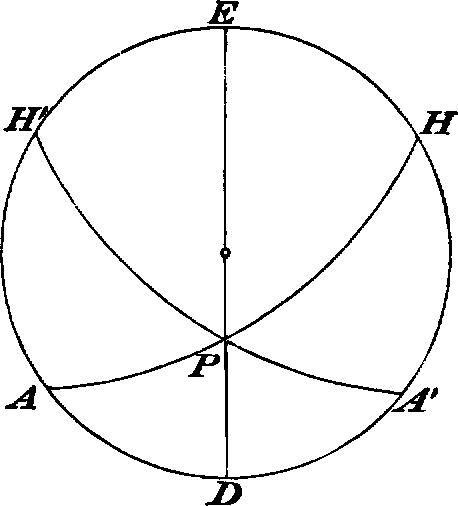
\includegraphics[width=5.0cm]{images/067fc}
\end{figure}

Let $ADA'E$ be a great circle; suppose $PA$ and $PA'$ the
projections on the plane of this circle of arcs which are each
equal to $b$ and inclined at an angle $A$ to $ADA'$; let $PD$ and
$PE$ be the projections of the least and greatest distances of $P$
from the great circle (see Art.\ 59). Thus the figure supposes
$A$ and $b$ each less than $\dfrac{\pi}{2}$.

If $a$ be less than the arc which is represented by $PD$ there is
no triangle; if $a$ be between $PD$ and $PA$ in magnitude, there are
two triangles, since $B$ will fall on $ADA'$, and we have two triangles
$BPA$ and $BPA'$; if $a$ be between $PA$ and $PH$ there will be only
one triangle, as $B$ will fall on $A'H$ or $AH'$, and the triangle will be
either $APB$ with $B$ between $A'$ and $H$, or else $A'PB$ with $B$ between
$A$ and $H'$; but these two triangles are symmetrically equal
(Art.\ 57); if $a$ be greater than $PH$ there will be no triangle.
The figure will easily serve for all the cases; thus if $A$ is greater
than $\dfrac{\pi}{2}$, we can suppose $PAE$ and $PA'E$ to be equal to $A$; if
$b$ is greater than $\dfrac{\pi}{2}$, we can take $PH$ and $PH'$ to represent $b$.
%-----File: 068.png------------------------------------------------

\paragraph{88.} The ambiguities which occur in the last case in the solution
of oblique-angled triangles (Art.\ 85) may be discussed in the
same manner as those in Art.\ 86; or, by means of the polar
triangle, the last case may be deduced from that of Art.~86.

\section*{\centering\normalsize EXAMPLES.}

1. The sides of a triangle are $105^\circ$, $90^\circ$, and $75^\circ$ respectively:
find the sines of all the angles.
\medskip

2. Shew that $\tan \tfrac{1}{2} A \tan \tfrac{1}{2} B= \dfrac{\sin(s-c)}{\sin s}$. Solve a triangle
when a side, an adjacent angle, and the sum of the other two
sides are given.
\medskip

3. Solve a triangle having given a side, an adjacent angle,
and the sum of the other two angles.
\medskip

4. A triangle has the sum of two sides equal to a semicircumference:
find the arc joining the vertex with the middle of
the base.
\medskip

5. If $a$, $b$, $c$ are known, $c$ being a \textit{quadrant}, determine the
angles: shew also that if $\delta$ be the perpendicular on $c$ from the
opposite angle, $\cos^2 \delta = \cos^2 a + \cos^2 b$.
\medskip

6. If one side of a spherical triangle be divided into four
equal parts, and $\theta_1$, $\theta_2$, $\theta_3$, $\theta_4$, be the angles subtended at the opposite
angle by the parts taken in order, shew that
\[
\sin(\theta_1 + \theta_2) \sin \theta_2 \sin\theta_4 = \sin(\theta_3 + \theta_4) \sin\theta_1 \sin\theta_3.
\]

7. In a spherical triangle if $A = B = 2C$, shew that
\[
8 \sin\left(a + \dfrac{c}{2}\right) \sin^2 \dfrac{c}{2} \cos \dfrac{c}{2} = \sin^3 a.
\]
%-----File: 069.png------------------------------------------------

8. In a spherical triangle if $A = B = 2C$, shew that
\[
8 \sin^2 \dfrac{C}{2} \left(\cos s + \sin \dfrac{C}{2}\right)
\dfrac{\cos\dfrac{c}{2}}{\cos a} = 1.
\]

9. If the equal sides of an isosceles triangle $ABC$ be bisected
by an arc $DE$, and $BC$ be the base, shew that
\[
\sin \dfrac{DE}{2} = \tfrac{1}{2} \sin \dfrac{BC}{2} \sec \dfrac{AC}{2}.
\]

10. If $c_1$, $c_2$ be the two values of the third side when $A$, $a$, $b$
are given and the triangle is ambiguous, shew that
\[
  \tan \dfrac{c_1}{2} \tan \dfrac{c_2}{2}
= \tan \tfrac{1}{2} (b - a) \tan \tfrac{1}{2} (b + a).
\]

\chapter[Circumscribed and Inscribed Circles.]{CIRCUMSCRIBED AND INSCRIBED CIRCLES.}

\paragraph{89.} \textit{To find the angular radius of the small circle inscribed
in a given triangle.}
\begin{figure}[htp]
\centering
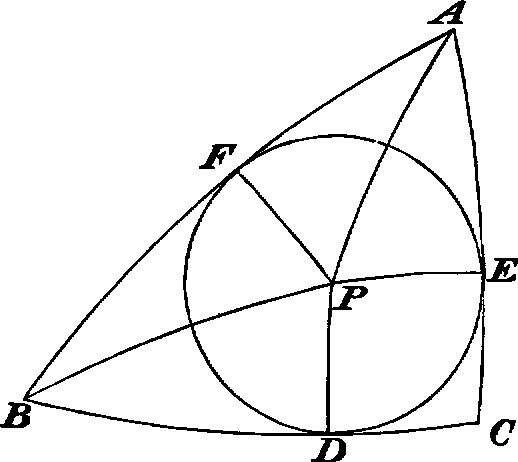
\includegraphics[width=5.0cm]{images/069fc}
\end{figure}

Let $ABC$ be the triangle; bisect the angles $A$ and $B$ by arcs
meeting at $P$; from $P$ draw $PD$, $PE$, $PF$ perpendicular to the
sides. Then it may be shewn that $PD$, $PE$, $PF$ are all equal;
also that $AE = AF$, $BF = BD$, $CD = CE$. Hence $BC + AF =$ half
the sum of the sides $= s$; therefore $AF = s - a$. Let $PF = r$.
\begin{flalign*}
&\rlap{\indent Now }&
  \tan PF &= \tan PAF \sin AF \text{ (Art.~62);} &&\\
&\rlap{thus }&
  \tan r  &= \tan\dfrac{A}{2} \sin (s-a). \tag{1}
\end{flalign*}
%-----File: 070.png------------------------------------------------

The value of $\tan r$ may be expressed in various forms; thus
from Art.~45, we obtain
\[
\tan \dfrac{A}{2} = \Surd {\frac{\sin (s - b) \sin (s - c)}{\sin s\, \sin (s - a)} } ;
\]
substitute this value in (1), thus
\[
\tan r = \Surd{\left\{
  \dfrac{\sin (s - a) \sin (s - b) \sin (s - c)}{\sin s} \right\}}
  = \dfrac{n}{\sin s} \text{ (Art.~46)}. \tag{2}
\]

Again
\begin{align*}
  \sin (s - a) &= \sin {\tfrac{1}{2}(b + c) - \tfrac{1}{2}a} \\[1ex]
    &= \sin \tfrac{1}{2}(b + c) \cos \tfrac{1}{2}a - \cos \tfrac{1}{2}(b + c) \sin \tfrac{1}{2}a \\[1ex]
    &= \dfrac{\sin \tfrac{1}{2}a \cos \tfrac{1}{2}a}{\sin \tfrac{1}{2}A}
        \{\cos \tfrac{1}{2}(B - C) - \cos \tfrac{1}{2}(B + C)\},\text{ (Art.~54)} \\[1ex]
    &= \dfrac{\sin a \sin \tfrac{1}{2}B \sin \tfrac{1}{2}C}{\sin \tfrac{1}{2}A};
\end{align*}
\begin{flalign*}
\text{therefore from (1) }&
\tan r = \dfrac{\sin\tfrac{1}{2}B \sin \tfrac{1}{2}C}{\cos \tfrac{1}{2}A} \sin a; \tag{3}&&
\end{flalign*}
hence, by Art.~51,
\begin{multline*}
\tan r =
\dfrac{\surd\{-\cos S \cos (S - A) \cos (S - B) \cos (S - C)\}}{2 \cos \tfrac{1}{2}A \cos \tfrac{1}{2}B \cos \tfrac{1}{2}C} \\[1ex]
=\frac{N}{2 \cos \tfrac{1}{2}A \cos \tfrac{1}{2}B \cos \tfrac{1}{2}C}. \tag{4}
\end{multline*}

It may be shewn by common trigonometrical formul\ae\ that
\[
4 \cos\tfrac{1}{2}A \cos\tfrac{1}{2}B \cos\tfrac{1}{2}C = \cos S + \cos (S - A) + \cos (S - B) + \cos (S - C);
\]
hence we have from (4)
\[
\cot r = \frac{1}{2N} \bigl\{\cos S + \cos (S - A) + \cos (S - B) + \cos (S - C)\bigr\}. \tag{5}
\]
%-----File: 071.png------------------------------------------------

\paragraph{90.} \textit{To find the angular radius of the small circle described
so as to touch one side of a given triangle, and the other sides
produced.}
\begin{figure}[htp]
\centering
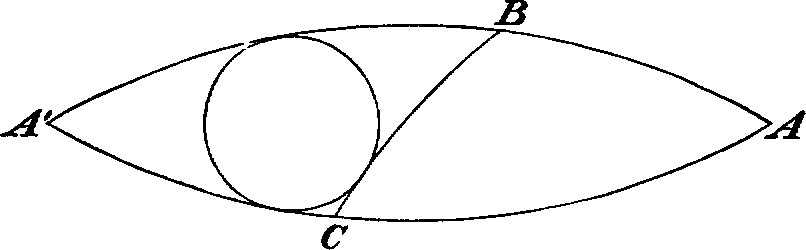
\includegraphics[width=5.0cm]{images/071fc}
\end{figure}

Let $ABC$ be the triangle; and suppose we require the radius
of the small circle which touches $BC$, and $AB$ and $AC$ produced.
Produce $AB$ and $AC$ to meet at $A'$; then we require the radius of
the small \textit{circle inscribed in $\mathrm{A'BC}$}, and the sides of $A'BC$ are $a$,
$\pi-b$, $\pi-c$ respectively. Hence if $r_1$ be the required radius, and
$s$ denote as usual $\frac{1}{2} (a + b + c)$, we have from Art.~89,
\[
  \tan r_1 = \tan\dfrac{A}{2}\sin s. \tag{1}
\]

From this result we may derive other equivalent forms as in
the preceding Article; or we may make use of those forms immediately,
observing that the angles of the triangle $A'BC$ are $A$,
$\pi-B$, $\pi-C$ respectively. Hence $s$ being $\frac{1}{2} (a + b + c)$ and $S$
being $\frac{1}{2} (A + B + C)$ we shall obtain
\begin{align*}
\tan r_1 &= \Surd{\left\{\dfrac{\sin s \sin(s-b)\sin(s-c)}
                         {\sin(s-a)}\right\}}
          = \dfrac{n}{\sin(s-a)}, \tag{2}
\\[1.5ex]
\tan r_1 &= \dfrac{\cos\tfrac{1}{2}B \cos\tfrac{1}{2}C}
                 {\cos\tfrac{1}{2}A} \sin a, \tag{3} \\[1ex]
\tan r_1 &
  \begin{gathered}[t]
  = \dfrac{\surd{\{-\cos S \cos(S-A) \cos(S-B) \cos(S-C)\}}}
         {2\cos\tfrac{1}{2}A \sin\tfrac{1}{2}B \sin\tfrac{1}{2}C} \notag
\\[1.5ex]
  = \dfrac{N}{2\cos\tfrac{1}{2}A \sin\tfrac{1}{2}B \sin\tfrac{1}{2}C},
  \end{gathered} \tag{4}
\\[1.5ex]
\multispan{2}{$\cot r_1 = \dfrac{1}{2N} \{-c\cos S - \cos(S-A) + \cos(S-B) + \cos(S-C) \} \tag{5}$.}
\end{align*}
%-----File: 072.png------------------------------------------------

These results may also be found independently by bisecting
two of the angles of the triangle $A'BC,$ so as to determine the
pole of the small circle, and proceeding as in Art.~89.

\paragraph{91.} A circle which touches one side of a triangle and the
other sides produced is called an \textit{escribed circle;} thus there are
three escribed circles belonging to a given triangle. We may
denote the radii of the escribed circles which touch $CA$ and $AB$
respectively by $r_2$ and $r_3$, and values of $\tan r_2$ and $\tan r_3$ may
be found from what has been already given with respect to
$\tan r_1$ by appropriate changes in the letters which denote the
sides and angles.

In the preceding Article a triangle $A'BC$ was formed by producing
$AB$ and $AC$ to meet again at $A'$; similarly another triangle
may be formed by producing $BC$ and $BA$ to meet again, and
another by producing $CA$ and $CB$ to meet again. The original
triangle $ABC$ and the three formed from it have been called
\textit{associated triangles}, $ABC$ being the fundamental triangle. Thus
the inscribed and escribed circles of a given triangle are the same
as the circles inscribed in the system of associated triangles of
which the given triangle is the fundamental triangle.

\paragraph{92.} \textit{To find the angular radius of the small circle described
about a given triangle.}
\begin{figure}[htp]
\centering
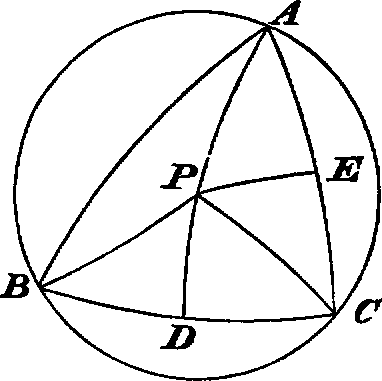
\includegraphics[width=5.0cm]{images/072fc}
\end{figure}

Let $ABC$ be the given triangle; bisect the sides $CB$, $CA$ at
$D$ and $E$ respectively, and draw from $D$ and $E$ arcs at right angles
to $CB$ and $CA$ respectively, and let $P$ be the intersection of these
%-----File: 073.png------------------------------------------------
arcs. Then $P$ will be the pole of the small circle described about
$ABC$. For draw $PA$, $PB$, $PC$; then from the right-angled
triangles $PCD$ and $PBD$ it follows that $PB=PC$; and from
the right-angled triangles $PCE$ and $PAE$ it follows that $PA = PC$;
hence $PA = PB=PC$. Also the angle $PAB =$ the angle $PBA$,
the angle $PBC =$ the angle $PCB$, and the angle $PCA =$ the angle
$PAC$; therefore $PCB + A = \tfrac{1}{2} (A + B + C)$, and $PCB = S-A$.

Let $PC = R$.
\begin{flalign*}
&\text{\indent Now }&
  \tan CD &= \tan CP \cos PCD,\ \text{(Art.\ 62,)}
  &\phantom{therefore }&\\[1ex]
&\text{thus }&
  \tan \tfrac{1}{2} a &= \tan R \cos (S-A),
  &&\\
&\text{therefore }&
  \tan R &= \dfrac{\tan\tfrac{1}{2}a}{\cos(S-A)}.
  \tag{1}
\end{flalign*}

The value of $\tan R$ may be expressed in various forms; thus
if we substitute for $\tan\dfrac{a}{2}$ from Art.~49, we obtain
\[
\tag{2}
\tan R
= \Surd{\left\{\dfrac{-\cos S}{\cos(S-A)\cos(S-B)\cos(S-C)}\right\}}
= \dfrac{\cos S}{N} \,.
\]
\begin{flalign*}
&\text{Again }&
  \cos(S-A) &= \cos\left\{\tfrac{1}{2}(B+C)-\tfrac{1}{2}A\right\}
&\phantom{Again }&
\\[1.5ex]
&&&= \cos\tfrac{1}{2}(B+C) \cos\tfrac{1}{2}A
   + \sin\tfrac{1}{2}(B+C) \sin\tfrac{1}{2}A
&&
\end{flalign*}
\vspace{-3ex}
\begin{align*}
\mspace{50mu}
&= \frac{\sin\tfrac{1}{2}A\cos\tfrac{1}{2}A}{\cos\tfrac{1}{2}a}
   \left\{\cos\tfrac{1}{2}(b+c)
         + \cos\tfrac{1}{2}(b-c) \right\},\ \text{(Art.\ 54,)}
\\
&= \dfrac{\sin A}{\cos\tfrac{1}{2}a} \cos\tfrac{1}{2}b\cos\tfrac{1}{2}c;
\end{align*}
therefore from (1)
\[
\tag{3}
\tan R = \dfrac{\sin\tfrac{1}{2}a }
              {\sin A\cos\tfrac{1}{2}b\cos\tfrac{1}{2}c } \,.
\]

Substitute in the last expression the value of $\sin A$ from
Art.~46; thus
\begin{align*}
\tan R
&= \dfrac{2\sin\tfrac{1}{2}a \sin\tfrac{1}{2}b \sin\tfrac{1}{2}c}
       {\surd{\left\{\sin s\sin(s-a) \sin(s-b) \sin(s-c) \right\}}}
\\[1.5ex]
&= \dfrac{2\sin\tfrac{1}{2}a \sin\tfrac{1}{2}b \sin\tfrac{1}{2}c}{n}
\,.
\tag{4} \\[-3ex]
\end{align*}
%-----File: 074.png------------------------------------------------

It may be shewn, by common trigonometrical formul\ae\, that
\[
  4\sin\tfrac{1}{2}a\sin\tfrac{1}{2}b\sin\tfrac{1}{2}c
= \sin(s-a) + \sin(s-b) + \sin(s-c)-\sin s;
\]
hence we have from (4)
\[
\tag{5}
\tan R=\dfrac{1}{2n}\{
\sin(s-a)+\sin(s-b)+\sin(s-c)-\sin s
\}.
\]

\paragraph{93.} \textit{To find the angular radii of the small circles described
round the triangles associated with a given fundamental triangle.}

Let $R_1$ denote the radius of the circle described round the
triangle formed by producing $AB$ and $AC$ to meet again at $A'$;
similarly let $R_2$ and $R_3$ denote the radii of the circles described
round the other two triangles which are similarly formed. Then
we may deduce expressions for $\tan R_1$, $\tan R_2$, and $\tan R_3$ from
those found in Art.~92 for $\tan R$. The sides of the triangle $A'BC$
are $a$, $\pi-b$, $\pi-c$, and its angles are $A$, $\pi-B$, $\pi-C$; hence if
$s = \tfrac{1}{2} (a + b + c)$ and $S = \tfrac{1}{2} (A + B + C)$ we shall obtain from
Art.~92
\begin{align*}
\tag{1}
  \tan R_1 &= \frac{\tan\frac{1}{2}a}{-\cos S} \,,
\\[1.5ex]
\tag{2}
  \tan R_1 &= \Surd{\left\{
  \frac{\cos(S-A)}{-\cos S\cos(S-B)\cos(S-C)}\right\}}
= \frac{\cos(S-A)}{N} \,,
\\[1.5ex]
\tag{3}
  \tan R_1 &= \frac{\sin\frac{1}{2}a}
                   {\sin A\sin\frac{1}{2}b\sin\frac{1}{2}c} \,,
\\[1.5ex]
\tag{4}
  \tan R_1
&= \frac{2\sin\frac{1}{2}a\cos\frac{1}{2}b\cos\frac{1}{2}c}
        {\surd{\{\sin s\sin(s-a)\sin(s-b)\sin(s-c)\}}} \,,
\\[1.5ex]
\tag{5}
  \tan R_1
&=\frac{1}{2n}
  \{\sin s - \sin(s-a) + \sin(s-b) + \sin(s-c) \}.
\end{align*}

Similarly we may find expressions for $\tan R_2$ and $\tan R_3$.

\paragraph{94.} Many examples may be proposed involving properties of
the circles inscribed in and described about the associated triangles.
We will give one that will be of use hereafter.
%-----File: 075.png------------------------------------------------

To prove that
\[(\cot r + \tan R)^2=\dfrac{1}{4n^2}(\sin a+\sin b+\sin c)^2 -1.\]

We have
\[
  4n^2=1-\cos^2 a-\cos^2 b-\cos^2 c+2\cos a\cos b\cos c;
\]
therefore
\[
(\sin a + \sin b + \sin c)^2-4n^2
\]
$= 2\ ( 1+ \sin a \sin b + \sin b \sin c + \sin c \sin a - \cos a \cos b \cos c \ )$.\\
Also $\cot r + \tan R
= \dfrac{1}{2n}\Bigl\{\sin s + \sin(s-a)+\sin(s-b)+\sin (s-c)\Bigr\}$;
and by squaring both members of this equation the required
result will be obtained. For it may be shewn by reduction that
\[
\sin^2 s + \sin^2 (s-a) + \sin^2 (s-b) + \sin^2 (s-c) = 2-2 \cos a \cos b \cos c,
\]
and
\begin{gather*}
\sin s \sin (s-a) + \sin s \sin (s-b) + \sin s \sin (s-c)
\\
{}+ \sin (s-a) \sin (s-b) + \sin (s-b) \sin (s-c) + \sin (s-c) \sin (s-a)
\\
= \sin a \sin b + \sin b \sin c + \sin c \sin a.
\end{gather*}

Similarly we may prove that
\[
(\cot r_1-\tan R)^2=\dfrac{1}{4n^2}(\sin b+\sin c-\sin a)^2 -1.
\]

\paragraph{95.} In the figure to Art.\ 89, suppose $DP$ produced through
$P$ to a point $A'$ such that $DA'$ is a quadrant, then $A'$ is a pole of
$BC$, and $PA' = \dfrac{\pi}{2}-r$; similarly, suppose $EP$ produced through $P$
to a point $B'$ such that $EB'$ is a quadrant, and $FP$ produced
through $P$ to a point $C'$ such that $FC'$ is a quadrant. Then
$A'B'C'$ is the polar triangle of $ABC$, and $PA' = PB' = PC' = \dfrac{\pi}{2}-r$.
Thus $P$ is the pole of the small circle \textit{described round} the polar
triangle, and the angular radius of the small circle described round
the polar triangle is the complement of the angular radius of the
%-----File: 076.png------------------------------------------------
small circle inscribed in the primitive triangle. And in like
manner the point which is the pole of the small circle inscribed in
the polar triangle is also the pole of the small circle described
round the primitive triangle, and the angular radii of the two
circles are complementary.

\section*{\centering\normalsize EXAMPLES.}

In the following examples the notation of the Chapter is
retained. Shew that in any triangle the following relations hold contained
in Examples 1 to 7:
\medskip

1. $\operatorname{Tan} r_1 \tan r_2 \tan r_3 = \tan r \sin^2 s$.
\medskip

2. $\operatorname{Tan} R + \cot r = \tan R_1 + \cot r_1 = \tan R_2 + \cot r_2$\\
\rightline{$= \tan R_3 + \cot r_3 = \tfrac{1}{2} (\cot r + \cot r_1 + \cot r_2 + \cot r_3)$.}
\medskip

3. $\operatorname{Tan}^2 R + \tan^2 R_1 + \tan^2 R_2 + \tan^2 R_3$\\
\rightline{$ = \cot^2 r + \cot^2 r_1 + \cot^2 r_2 + \cot^2 r_3$.}
\medskip

4. $\dfrac{\operatorname{Tan} r_1 + \tan r_2 + \tan r_3 - \tan r}
       {\cot r_1 + \cot r_2 + \cot r_3 - \cot r}
= \tfrac{1}{2} (1 + \cos a + \cos b + \cos c)$.
\medskip

5. $\operatorname{Cosec}^2 r
= \cot (s - a) \cot (s - b)
+ \cot (s - b) \cot (s - c)
+ \cot (s - c)      (s - a)$.
\medskip

6. $\operatorname{Cosec}^2 r_1
= \cot (s - b) \cot (s - c)
- \cot s \cot (s - b)
- \cot s \cot (s - c)$.
\medskip

7. $\operatorname{Tan} R_1 \tan R_2 \tan R_3 = \tan R \sec^2 S$.
\medskip

8. Shew that in an equilateral triangle $\tan R = 2\tan r$.
\medskip

9. If $ABC$ be an equilateral spherical triangle, $P$ the pole of
the circle circumscribing it, $Q$ any point on the sphere, shew that
\[
  \cos QA + \cos QB + \cos QC = 3\cos PA \cos PQ.
\]

10. If three small circles be inscribed in a spherical triangle
having each of its angles $120^\circ$, so that each touches the other two
as well as two sides of the triangle, shew that the radius of each
of the small circles $= 30^\circ$, and that the centres of the three small
circles coincide with the angular points of the polar triangle.
%-----File: 077.png------------------------------------------------

\chapter[Area of a Spherical Triangle. Spherical Excess.]{AREA OF A SPHERICAL TRIANGLE\@. SPHERICAL EXCESS.}

\paragraph{96.} \textit{To find the area of a Lune.}

A \textit{Lune} is that portion of the surface of a sphere which is
comprised between two great semicircles.
\begin{figure}[htp]
\centering
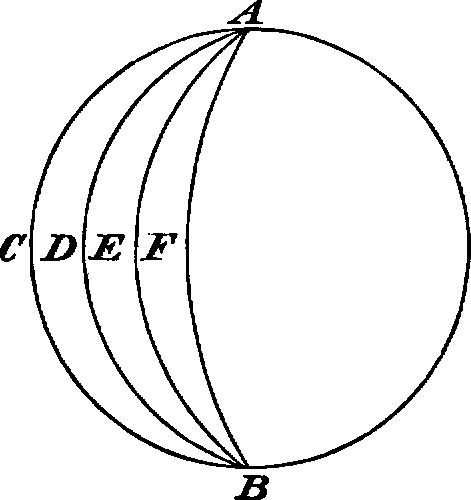
\includegraphics[width=5.0cm]{images/077fc}
\end{figure}

Let $ACBDA$, $ADBEA$ be two lunes having equal angles at $A$;
then one of these lunes may be supposed placed on the other so as
to coincide exactly with it; thus \textit{lunes having equal angles are
equal.} Then by a process similar to that used in the first proposition
of the Sixth Book of Euclid it may be shewn that \textit{lunes
are proportional to their angles.} Hence since the whole surface of
a sphere may be considered as a lune with an angle equal to four
right angles, we have for a lune with an angle of which the
circular measure is $A$,
\[
  \dfrac{\text{area of lune}}{\text{surface of sphere}}
= \dfrac{A}{2\pi}\,.
\]

Suppose $r$ the radius of the sphere, then the surface is $4\pi r^2$
(\textit{Integral Calculus}, Chap.~\textsc{vii.}); thus
\[
  \text{area of lune } = \dfrac{A}{2\pi} 4\pi r^2 = 2Ar^2.
\]
%-----File: 078.png------------------------------------------------

\paragraph{97.} \textit{To find the area of a Spherical Triangle.}
\begin{figure}[htp]
\centering
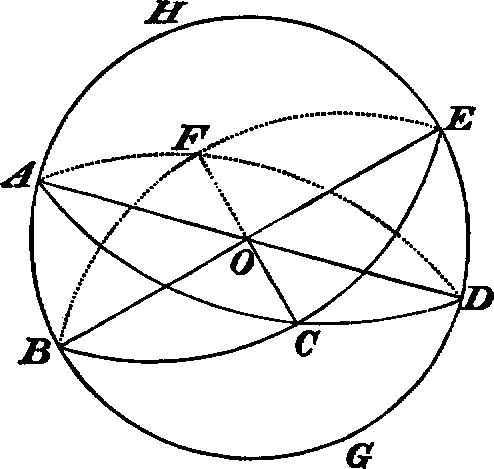
\includegraphics[width=5.0cm]{images/078fc}
\end{figure}

Let $ABC$ be a spherical triangle; produce the arcs which form
its sides until they meet again two and two, which will happen
when each has become equal to the semicircumference. The
triangle $ABC$ now forms a part of three lunes, namely, $ABDCA$,
$BCEAB$, and $CAFBC$. Now the triangles $CDE$ and $AFB$ are
subtended by vertically opposite solid angles at $O$, and \textit{we will
assume} that their areas are equal; therefore the lune $CAFBC$ is
equal to the sum of the two triangles $ABC$ and $CDE$. Hence if
$A$, $B$, $C$ denote the circular measures of the angles of the triangle,
we have
\begin{align*}
& \text{triangle } ABC+BGDC = \text{lune } ABDCA = 2Ar^2, \\
& \text{triangle } ABC+AHEC = \text{lune } BCEAB = 2Br^2, \\
& \text{triangle } ABC+\text{triangle } CDE
= \text{lune } CAFBC = 2Cr^2;
\end{align*}
hence, by addition,
\[
  \text{twice triangle } ABC + \text{surface of hemisphere}
= 2(A+B+C)r^2;
\]
$\rlap{therefore }\hfill
  \text{triangle } ABC=(A+B+C-\pi)r^2.
\hfill$

The expression $A+B+C-\pi$ is called the \textit{spherical excess} of
the triangle; and since
\[
  (A+B+C-\pi)r^2 = \dfrac{A+B+C-\pi}{2\pi}\, 2\pi r^2,
\]
%-----File: 079.png------------------------------------------------
the result obtained may be thus enunciated: \textit{the area of a spherical
triangle is the same fraction of half the surface of the sphere as the
spherical excess is of four right angles.}

\paragraph{98.} We have assumed, as is usually done, that the areas of
the triangles $CDE$ and $AFB$ in the preceding Article are equal.
The triangles are, however, not absolutely equal, but \textit{symmetrically}
equal (Art.\ 57), so that one cannot be made to coincide
with the other by superposition. It is, however, easy to decompose
two such triangles into pieces which admit of superposition,
and thus to prove that their areas are equal. For describe a
small circle round each, then the angular radii of these circles
will be equal by Art.~92. If the pole of the circumscribing circle
falls inside each triangle, then each triangle is the sum of three
isosceles triangles, and if the pole falls outside each triangle, then
each triangle is the excess of two isosceles triangles over a third;
and in each case the isosceles triangles of one set are respectively
\textit{absolutely equal} to the corresponding isosceles triangles of the
other set.

\paragraph{99.} \textit{To find the area of a spherical polygon.}

Let $n$ be the number of sides of the polygon, $\Sigma$ the sum of all
its angles. Take any point within the polygon and join it with
all the angular points; thus the figure is divided into $n$ triangles.
Hence, by Art.~97,
\[
  \text{area of polygon
= (sum of the angles of the triangles} - n\pi)r^2,
\]
and the sum of the angles of the triangles is equal to $\Sigma$ together
with the four right angles which are formed round the common
vertex; therefore
\[
  \text{area of polygon} = \Bigl\{\Sigma - (n-2)\pi \Bigr\} r^2.
\]

This expression is true even when the polygon has some of its
angles greater than two right angles, provided it can be decomposed
into triangles, of which each of the angles is less than two
right angles.
%-----File: 080.png------------------------------------------------

\paragraph{100.} We shall now give some expressions for certain trigonometrical
functions of the \textit{spherical excess} of a triangle. We denote
the spherical excess by $E$, so that $E=A+B+C-\pi$.

\paragraph{101.} \textit{Cagnoli's Theorem.} To shew that
\[
  \sin\tfrac{1}{2}E
= \dfrac{\surd\{\sin s \sin(s-a) \sin(s-b) \sin(s-c) \} x}
{2\cos\tfrac{1}{2}a \cos\tfrac{1}{2}b \cos\tfrac{1}{2}c }.
\]
\begin{align*}
   \operatorname{Sin}\tfrac{1}{2}E
&= \sin\tfrac{1}{2}(A+B+C-\pi)
 = \sin\{\tfrac{1}{2}(A+B) - \tfrac{1}{2}(\pi-C) \}
\\[1.5ex]
&= \sin\tfrac{1}{2}(A+B) \sin\tfrac{1}{2}C
 - \cos\tfrac{1}{2}(A+B) \cos\tfrac{1}{2}C
\\[1.5ex]
&= \dfrac{\sin\tfrac{1}{2}C \cos\tfrac{1}{2}C }{\cos\tfrac{1}{2}c }
   \{\cos\tfrac{1}{2}(a-b) - \cos\tfrac{1}{2}(a-b) \},
   \quad \text{(Art.~54),}
\\[1.5ex]
&= \dfrac{\sin C \sin\tfrac{1}{2}a \sin\tfrac{1}{2}b }{\cos\tfrac{1}{2}c}
\\[1.5ex]
&= \frac{\sin\tfrac{1}{2}a\sin\tfrac{1}{2}b}{\cos\tfrac{1}{2}c}\centerdot
   \frac{2}{\sin a\sin b} \centerdot
   \surd\{\sin s\sin(s-a)\sin(s-b)\sin(s-c) \}\\
&= \frac{\surd\{\sin s\sin(s-a)\sin(s-b)\sin(s-c) \} }
        {2\cos\tfrac{1}{2}a \cos\tfrac{1}{2}b \cos\tfrac{1}{2}c }.
\end{align*}

\paragraph{102.} \textit{Lhuilier's Theorem.} To shew that
\begin{flalign*}
&&\tan\tfrac{1}{4}E
&= \surd\{\tan\tfrac{1}{2}s \tan\tfrac{1}{2}(s-a)
       \tan\tfrac{1}{2}(s-b) \tan\tfrac{1}{2}(s-c) \}.
\\[3ex]
&&\operatorname{Tan}\tfrac{1}{4}E
&= \dfrac{\sin\tfrac{1}{2}(A+B+C-\pi) }
        {\cos\tfrac{1}{4}(A+B+C-\pi) }
\\[1.5ex]
&&&= \dfrac{\sin\tfrac{1}{2}(A+B) - \sin\tfrac{1}{2}(\pi-C) }
          {\cos\tfrac{1}{2}(A+B) + \cos\tfrac{1}{2}(\pi-C) }\,,
&\llap{(\textit{Plane Trig.}~Art.~84),}&
\\[1.5ex]
&&&= \dfrac{\sin\tfrac{1}{2}(A+B) - \cos\tfrac{1}{2}C }
          {\cos\tfrac{1}{2}(A+B) + \sin\tfrac{1}{2}C }
\\[1.5ex]
&&&= \dfrac{\cos\tfrac{1}{2}(a-b) - \cos\tfrac{1}{2}c }
          {\cos\tfrac{1}{2}(a+b) + \cos\tfrac{1}{2}c } \centerdot
     \dfrac{\cos\tfrac{1}{2}C }{\sin\tfrac{1}{2}C }\,,
&\llap{(Art.~54)}.&
\end{flalign*}

Hence, by Art.~45, we obtain
\begin{align*}
\tan\tfrac{1}{4}E
&= \dfrac{\sin\tfrac{1}{4}(c+a-b) \sin\tfrac{1}{4}(c+b-a) }
        {\cos\tfrac{1}{4}(a+b+c) \cos\tfrac{1}{4}(a+b-c) }
   \Surd{\left\{
          \dfrac{\sin s\sin(s-c) }{\sin(s-a)\sin(s-b) } \right\} }
\\[1.5ex]
&= \surd\{\tan\tfrac{1}{2}s \tan\tfrac{1}{2}(s-a)
           \tan\tfrac{1}{2}(s-b) \tan\tfrac{1}{2}(s-c) \}.
\end{align*}
%-----File: 081.png------------------------------------------------

\paragraph{103.} We may obtain many other formul\ae\ involving trigonometrical
functions of the spherical excess. Thus, for example,
\begin{align*}
\cos\tfrac{1}{2}E
&= \cos\left\{\tfrac{1}{2}(A+B)
 - \tfrac{1}{2}(\pi-C) \right\}
\\[1.5ex]
&= \cos\tfrac{1}{2}(A+B) \sin\tfrac{1}{2}C +
   \sin\tfrac{1}{2}(A+B) \cos\tfrac{1}{2}C
\\[1.5ex]
&= \Bigl\{\cos\tfrac{1}{2}(a+b) \sin^2\tfrac{1}{2}C +
           \cos\tfrac{1}{2}(a-b) \cos^2\tfrac{1}{2}C \Bigr\}
   \sec\tfrac{1}{2}c,\ \text{(Art.\ 54),}
\\[1.5ex]
&= \Bigl\{\cos\tfrac{1}{2}a \cos\tfrac{1}{2}b
   (\cos^2C + \sin^2\tfrac{1}{2}C)
\\
&\mspace{100mu}
{}+\sin\tfrac{1}{2}a \sin\tfrac{1}{2}b
   (\cos^2\tfrac{1}{2}C - \sin^2\tfrac{1}{2}C) \Bigr\}
   \sec\tfrac{1}{2}c
\\[1.5ex]
&=\left\{\cos\tfrac{1}{2}a \cos\tfrac{1}{2}b +
          \sin\tfrac{1}{2}a \sin\tfrac{1}{2}b \cos C \right\}
  \sec\tfrac{1}{2}c.
\tag{1}
\end{align*}

Again, it was shewn in Art.\ 101, that
\begin{flalign*}
&&& \sin\tfrac{1}{2}E
  = \sin C \sin\tfrac{1}{2}a \sin\tfrac{1}{2}b \sec\tfrac{1}{2}c; &&
\\[1.5ex]
&\rlap{therefore}&
\tag{2}
& \tan\tfrac{1}{2}E =
  \frac{\sin\tfrac{1}{2}a \sin\tfrac{1}{2}b \sin C }
       {\cos\tfrac{1}{2}a \cos\tfrac{1}{2}b
       + \sin\tfrac{1}{2}a \sin\tfrac{1}{2}b \cos C } \,.
\end{flalign*}

Again, we have from above
\[
  \cos\tfrac{1}{2}E
= \Bigl\{\cos\tfrac{1}{2}a \cos\tfrac{1}{2}b
        + \sin\tfrac{1}{2}a \sin\tfrac{1}{2}b \cos C \Bigr\}
  \sec\tfrac{1}{2}c
\]
\begin{align*}
&= \dfrac{(1+\cos a)(1+\cos b) + \sin a\sin b\cos C}
        {4\cos\tfrac{1}{2}a \cos\tfrac{1}{2}b \cos\tfrac{1}{2}c }
\\[1.5ex]
&= \dfrac{1+\cos a+\cos b\cos c }
        {4\cos\tfrac{1}{2}a \cos\tfrac{1}{2}b \cos\tfrac{1}{2}c }
 = \frac{\cos^2\tfrac{1}{2}a + \cos^2\tfrac{1}{2}b
        + \cos^2\tfrac{1}{2}c-1 }
        {2\cos\tfrac{1}{2}a \cos\tfrac{1}{2}b \cos\tfrac{1}{2}c }
\tag{3} \,.
\end{align*}

In (3) put $1-2\sin^2\frac{1}{4}E$ for $\cos \frac{1}{2}E$; thus
\[
\sin^2\tfrac{1}{4}E =
  \dfrac{1 + 2\cos\tfrac{1}{2}a \cos\tfrac{1}{2}b \cos\tfrac{1}{2}c
       - \cos^2\tfrac{1}{2}a - \cos^2\tfrac{1}{2}b - \cos^2\tfrac{1}{2}c}
       {4\cos\tfrac{1}{2}a \cos\tfrac{1}{2}b \cos\tfrac{1}{2}c }\,.
\]

By ordinary development we can shew that the numerator of
the above fraction is equal to
\[
  4\sin\tfrac{1}{2}s \sin\tfrac{1}{2}(s-a)
   \sin\tfrac{1}{2}(s-b) \sin\tfrac{1}{2}(s-c);
\]
%-----File: 082.png------------------------------------------------
therefore
\begin{align*}
\sin^2\tfrac{1}{4}E
&= \frac{\sin\frac{1}{2}s \sin\frac{1}{2}(s-a)
          \sin\frac{1}{2}(s-b) \sin\frac{1}{2}(s-c) }
        {\cos\frac{1}{2}a \cos\frac{1}{2}b \cos\frac{1}{2}c }.\tag{4}\\
\intertext{\indent Similarly}
\cos^2\tfrac{1}{4}E
&= \frac{\cos\frac{1}{2}s \cos\frac{1}{2}(s-a)
          \cos\frac{1}{2}(s-b) \cos\frac{1}{2}(s-c) }
        {\cos\frac{1}{2}a \cos\frac{1}{2}b \cos\frac{1}{2}c }.\tag{5}
\end{align*}

Hence by division we obtain Lhuilier's Theorem.

Again,
\begin{multline*}
\frac{\sin(C-\tfrac12E)}{\sin\frac12E} = \sin C\cot\tfrac12E-\cos C\\
\begin{aligned}
&= \sin C \frac{\cos\frac12a \cos\frac12b
               + \sin\frac12a \sin\frac12b \cos C}
               {\sin\frac12a \sin\frac12b \sin C}
 - \cos C, \text{ by (2),}
\\
&=\cos\tfrac12a \cot\tfrac12b;
\end{aligned}
\end{multline*}
therefore, by Art.\ 101,
\[
  \sin(C-\tfrac12E)
= \frac{\surd\{\sin s \sin(s-a) \sin(s-b) \sin(s-c) \} }
       {2\sin\frac12a \sin\frac12b \cos\frac12c }.
\]

Again, $\cos(C-\frac12E)=\cos C\cos\frac12E+\sin C\sin\frac12E$
\begin{align*}
&= \frac{(1+\cos a)(1+\cos b)\cos C + \sin a\sin b\cos^2 C }
        {4\cos\frac12a \cos\frac12b \cos\frac12c }
 + \sin^2C \sin\tfrac12a \sin\tfrac12b \sec\tfrac12c
\\[1.5ex]
&= \frac{(1+\cos a)(1+\cos b)\cos C + \sin a\sin b }
        {4\cos\frac12a \cos\frac12b \cos\frac12c }
\\[1.5ex]
&= \Bigl\{\cos\tfrac12a \cos\tfrac12b \cos C
         + \sin\tfrac12a \sin\tfrac12b \Bigr\} \sec\tfrac12c
\\[1.5ex]
&= \frac{\sin a\sin b\cos C + 4\sin^2\frac12a \sin^2\frac12b }
        {4\sin\frac12a \sin\frac12b \cos\frac12c }
\\[1.5ex]
&= \frac{\cos c - \cos a\cos b + (1-\cos a)(1-\cos b) }
        {4\sin\frac12a \sin\frac12b \cos\frac12c }
\\[1.5ex]
&= \frac{1 + \cos c - \cos a - \cos b }
        {4\sin\frac12a \sin\frac12b \cos\frac12c }
 = \frac{\cos^2\frac12c - \cos^2\frac12a - \cos^2\frac12b + 1 }
        {2\sin\frac12a \sin\frac12b \cos\frac12c }\,.\tag{6}
\end{align*}
%-----File: 083.png------------------------------------------------

From this result we can deduce two other results, in the
same manner as (4) and (5) were deduced from (3); or we may
observe that the right-hand member of (6) can be obtained from
the right-hand member of (3) by writing $\pi-a$ and $\pi-b$ for
$a$ and $b$ respectively, and thus we may deduce the results more
easily. We shall have then
\begin{align*}
\sin^2 (\tfrac{1}{2}C-\tfrac{1}{4}E) &=
  \frac{\cos\frac{1}{2}s \sin\frac{1}{2}(s-a) \sin\frac{1}{2}(s-b) \cos\frac{1}{2}(s-c) }
       {\sin\frac{1}{2}a \sin\frac{1}{2}b \cos\frac{1}{2}c },
\\[1.5ex]
\cos^2 (\tfrac{1}{2}C-\tfrac{1}{4}E) &=
  \frac{\sin\frac{1}{2}s \cos\frac{1}{2}(s-a) \cos\frac{1}{2}(s-b) \sin\frac{1}{2}(s-c) }
       {\sin\frac{1}{2}a \sin\frac{1}{2}b \cos\frac{1}{2}c }.
\end{align*}

\section*{\centering\normalsize EXAMPLES.}

1. Find the angles and sides of an equilateral triangle whose
area is one-fourth of that of the sphere on which it is described.
\medskip

2. Find the surface of an equilateral and equiangular spherical
polygon of $n$ sides, and determine the value of each of the
angles when the surface equals half the surface of the sphere.
\medskip

3. If $a=b=\dfrac{\pi}{3}$, and $c=\dfrac{\pi}{2}$, shew that $E=\cos^{-1}\dfrac{7}{9}$.
\medskip

4. If the angle $C$ of a spherical triangle be a right angle,
shew that
\[
\sin \tfrac{1}{2} E= \sin \tfrac{1}{2} a \sin \tfrac{1}{2} b \sec \tfrac{1}{2} c, \quad
\cos \tfrac{1}{2} E= \cos \tfrac{1}{2} a \cos \tfrac{1}{2} b \sec \tfrac{1}{2} c.
\]

5. If the angle $C$ be a right angle, shew that
\[
\frac{\sin^2 c}{\cos c}\cos E= \frac{\sin^2 a}{\cos a}+\frac{\sin^2 b}{\cos b}.
\]

6. If $a=b$ and $C=\dfrac{\pi}{2}$, shew that $\tan E=\dfrac{\sin^2 a}{2\cos a}$.
\medskip

7. The sum of the angles in a right-angled triangle is less
than four right angles.
\medskip

8. Draw through a given point in the side of a spherical
triangle an arc of a great circle cutting off a given part of the
triangle.
%-----File: 084.png------------------------------------------------
\medskip

9. In a spherical triangle if $\cos C=1\tan\dfrac{a}{2}\tan\dfrac{b}{2}$, then
$C=A+B$.
\medskip

10. If the angles of a spherical triangle be together equal to
four right angles
\[
  \cos^2\tfrac{1}{2}a + \cos^2\tfrac{1}{2}b + \cos^2\tfrac{1}{2}c = 1.
\]

11. If $r_1$, $r_2$, $r_3$ be the radii of three small circles of a
sphere of radius $r$ which touch one another at $P$, $Q$, $R$, and
$A$, $B$, $C$ be the angles of the spherical triangle formed by joining
their centres,
\[
\text{area }PQR = (A\cos r_1 + B\cos r_2 + C\cos r_3 - \pi)r^2.
\]

12. Shew that
\[
\sin s
= \frac{\Bigl\{\sin\frac{1}{2}E \sin(A-\frac{1}{2}E)
         \sin(B-\frac{1}{2}E) \sin(C-\frac{1}{2}E)
         \Bigr\}^{\frac{1}{2}} }
       {2\sin\frac{1}{2}A \sin\frac{1}{2}B \sin\frac{1}{2}C } \,.
\]

13. Given two sides of a spherical triangle, determine when
the area is a maximum.
\medskip

14. Find the area of a regular polygon of a given number of
sides formed by arcs of great circles on the surface of a sphere;
and hence deduce that, if $\alpha$ be the angular radius of a small
circle, its area is to that of the whole surface of the sphere as
$\operatorname{versin}\alpha$ is to 2.
\medskip

15. $A$, $B$, $C$ are the angular points of a spherical triangle;
$A'$, $B'$, $C'$ are the middle points of the respectively opposite sides.
If $E$ be the spherical excess of the triangle, shew that
\[
  \cos\tfrac{1}{2}E
= \frac{\cos A'B'}{\cos \frac{1}{2}c}
= \frac{\cos B'C'}{\cos \frac{1}{2}a}
= \frac{\cos C'A'}{\cos \frac{1}{2}b}\,.
\]

16. If one of the arcs of great circles which join the middle
points of the sides of a spherical triangle be a quadrant, shew that
the other two are also quadrants.
%-----File: 085.png------------------------------------------------

\chapter[On certain approximate Formul\ae.]{ON CERTAIN APPROXIMATE FORMUL\AE.}

\paragraph{104.} We shall now investigate certain approximate formul\ae\
which are often useful in calculating spherical triangles when the
radius of the sphere is large compared with the lengths of the
sides of the triangles.

\paragraph{105.} \textit{Given two sides and the included angle of a spherical
triangle, to find the angle between the chords of these sides.}
\begin{figure}[htp]
\centering
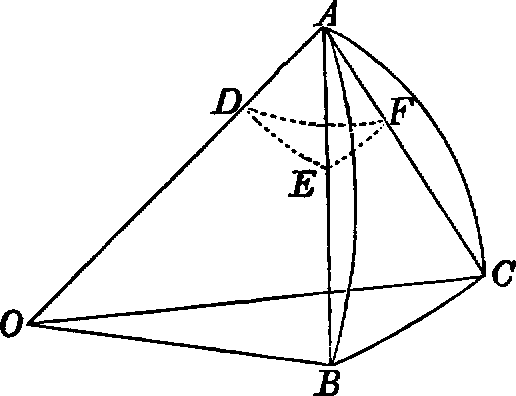
\includegraphics[width=5.0cm]{images/085fc}
\end{figure}

Let $AB$, $AC$ be the two sides of the triangle $ABC$; let $O$ be
the centre of the sphere. Describe a sphere round $A$ as a centre,
and suppose it to meet $AO$, $AB$, $AC$ at $D$, $E$, $F$ respectively.
Then the angle $EDF$ is the inclination of the planes $OAB$, $OAC$,
and is therefore equal to $A$. From the spherical triangle $DEF$\\[1ex]
${} \hfill \cos EF=\cos DE \cos DF + \sin DE \sin DF \cos A; \hfill$\\[1ex]
$\rlap{and }\hfill
  DE = \frac{1}{2} (\pi - c),\quad
  DF = \frac{1}{2} (\pi - b);\hfill$\\[1ex]
$\rlap{therefore }\hfill
  \cos EF = \sin \frac{1}{2} b \sin \frac{1}{2} c
          + \cos \frac{1}{2} b \cos \frac{1}{2} c \cos A. \hfill$

If the sides of the triangle are small compared with the
radius of the sphere, $EF$ will not differ much from $A$; suppose
$EF=A - \theta$, then approximately
\[
  \cos EF = \cos A + \theta \sin A;
\]
%-----File: 086.png------------------------------------------------
\begin{flalign*}
&\text{and}&\sin\tfrac12b \sin\tfrac12c &= \sin^2\tfrac14(b + c) - \sin^2\tfrac14(b - c),&\phantom{and}\\[1.5ex]
&&\cos\tfrac12b \cos\tfrac12c &= \cos^2\tfrac14(b + c) - \sin^2\tfrac14(b - c);
\end{flalign*}
therefore
\begin{multline*}
\cos A + \theta\sin A = \sin^2\tfrac14(b + c) - \sin^2\tfrac14(b - c)\\
{}+ \Bigl\{1 - \sin^2\tfrac14(b + c) - \sin^2\tfrac14(b - c)\Bigr\}\cos A;
\end{multline*}
therefore
\[
  \theta\sin A = (1 - \cos A)\sin^2\tfrac14(b + c)
                 - (1 + \cos A)\sin^2\tfrac14(b - c),
\]
therefore \hfill$%
  \theta = \tan\tfrac12A \sin^2\tfrac14(b + c)
         - \cot\tfrac12A \sin^2\tfrac14(b - c).
\hfill\phantom{therefore}$

This gives the \textit{circular measure} of $\theta$; the number of seconds in
the angle is found by dividing the circular measure by the circular
measure of one second, or approximately by the sine of one second
(\textit{Plane Trigonometry}, Art.\ 123). If the lengths of the arcs corresponding
to $a$ and $b$ respectively be $\alpha$ and $\beta$, and $r$ the radius of the
sphere, we have $\dfrac{\alpha}{r}$ and $\dfrac{\beta}{r}$ as the circular measures of $a$ and $b$
respectively; and the lengths of the sides of the chordal triangle
are $2r\sin\dfrac{\alpha}{2r}$ and $2r\sin\dfrac{\beta}{2r}$ respectively. Thus when the sides of
the spherical triangle and the radius of the sphere are known, we
can calculate the angles and sides of the chordal triangle.

\paragraph{106.} Legendre's Theorem. \textit{If the sides of a spherical triangle
be small compared with the radius of the sphere, then each angle
of the spherical triangle exceeds by one third of the spherical excess
the corresponding angle of the plane triangle, the sides of
which are of the same length as the arcs of the spherical triangle.}

Let $A$, $B$, $C$ be the angles of the spherical triangle; $a$, $b$, $c$
the sides; $r$ the radius of the sphere; $\alpha$, $\beta$, $\gamma$ the lengths of the
arcs which form the sides, so that $\dfrac{\alpha}{r}$, $\dfrac{\beta}{r}$, $\dfrac{\gamma}{r}$ are the circular
measures of $a$, $b$, $c$ respectively. Then
%-----File: 087.png------------------------------------------------
\begin{flalign*}
&& \cos A &= \frac{\cos a - \cos b\cos c}{\sin b \sin c}\,; &&\\
&\text{now }& \cos a
&= 1 - \frac{\alpha^2}{2r^2} + \frac{\alpha^4}{24r^4} - \ldots, &\phantom{text}&\\
&& \sin a &=\frac{\alpha}{r} - \frac{\alpha^3}{6r^3} +\ldots.
\end{flalign*}

Similar expressions hold for $\cos b$ and $\sin b$, and for $\cos c$
and $\sin c$ respectively. Hence, if we neglect powers of the circular
measure above the \textit{fourth}, we have
\begin{align*}
\cos A
&=\frac{1 -\dfrac{\alpha^2}{2r^2} +\dfrac{\alpha^4}{24r^4}
 - \left( 1 -\dfrac{\beta^2}{2r^2} +\dfrac{\beta^4}{24r^4} \right)
   \left( 1 -\dfrac{\gamma^2}{2r^2} +\dfrac{\gamma^4}{24r^4} \right)}
        {\dfrac{\beta\gamma}{r^2}
          \left( 1 - \dfrac{\beta^2}{6r^2} \right)
          \left( 1 - \dfrac{\gamma^2}{6r^2} \right)}
\\[1.5ex]
&=\frac{\dfrac{1}{2r^2}(\beta^2 + \gamma^2 - \alpha^2)
        + \dfrac{1}{24r^4}
          (\alpha^4 - \beta^4 - \gamma^4 - 6\beta^2\gamma^2)}
        {\dfrac{\beta\gamma}{r^2}
          \left( 1 - \dfrac{\beta^2 + \gamma^2}{6r^2} \right)}
\\[1.5ex]
&=\frac{1}{2\beta\gamma}
  \left\{\beta^2 + \gamma^2 - \alpha^2
        + \dfrac{1}{12r^2}
          (\alpha^2 - \beta^2 - \gamma^2 - 6\beta^2\gamma^2) \right\}
  \left\{1 + \dfrac{\beta^2 + \gamma^2}{6r^2} \right\}
\\[2ex]
&=\dfrac{\beta^2 + \gamma^2 - \alpha^2}{2\beta\gamma}
 +\dfrac{\alpha^4 + \beta^4 + \gamma^4
        - 2\alpha^2\beta^2 - 2\beta^2\gamma^2 - 2\gamma^2\alpha^2}
        {24\beta\gamma r^2}\,.
\end{align*}

Now let $A'$, $B'$, $C'$ be the angles of the plane triangle whose
sides are $\alpha$, $\beta$, $\gamma$ respectively; then
\begin{flalign*}
&& \cos A' &= \frac{\beta^2 + \gamma^2 - \alpha^2}{2 \beta \gamma}\,,\\
&\text{thus}&
  \cos A &= \cos A' - \frac{\beta \gamma \sin^2 A'}{6r^2}\,.
&\phantom{thus}&
\end{flalign*}

Suppose $A = A' + \theta$; then
\[
  \cos A = \cos A' - \theta \sin A' \text{ approximately};
\]
$\text{therefore} \hfill\displaystyle
  \theta = \frac{\beta \gamma \sin A'}{6r^2}=\frac{S}{3r^2}\,,\hfill \phantom{therefore}$\\[1ex]
%-----File: 088.png------------------------------------------------
where $S$ denotes the area of the plane triangle whose sides are
$\alpha$, $\beta$, $\gamma$. Similarly
\[
B = B' + \frac{S}{3r^2} \text{ and } C = C' + \frac{S}{3r^2}\,;
\]
hence approximately
\[
A+B+C = A'+B'+C'+\frac{S}{r^2} = \pi + \frac{S}{r^2}\,;
\]
therefore $\dfrac{S}{r^2}$ is approximately equal to the spherical excess of the
spherical triangle, and thus the theorem is established.

It will be seen that in the above approximation the area of
the spherical triangle is considered equal to the area of the plane
triangle which can be formed with sides of the same length.

\paragraph{107.} Legendre's Theorem may be used for the approximate
solution of spherical triangles in the following manner.

(1) Suppose the three sides of a spherical triangle known;
then the values of $\alpha$, $\beta$, $\gamma$ are known, and by the formul\ae\ of
Plane Trigonometry we can calculate $S$ and $A'$, $B'$, $C'$; then
$A$, $B$, $C$ are known from the formul\ae.
\[
A = A' + \frac{S}{3r^2}, \quad
B = B' + \frac{S}{3r^2}, \quad
C = C' + \frac{S}{3r^2}.
\]

(2) Suppose two sides and the included angle of a spherical
triangle known, for example $A$, $b$, $c$. Then
\[
S = \tfrac{1}{2}\beta\gamma\sin A' = \tfrac{1}{2}\beta\gamma\sin A \text{ approximately.}
\]
Then $A'$ is known from the formula $A'=A-\dfrac{S}{3r^2}$. Thus in the
plane triangle two sides and the included angle are known;
therefore its remaining parts can be calculated, and then those
of the spherical triangle become known.
%-----File: 089.png------------------------------------------------

(3) Suppose two sides and the angle opposite to one of them
in a spherical triangle known, for example $A$, $a$, $b$. Then
\[
\sin B' = \frac{\beta}{\alpha}\sin A' = \frac{\beta}{\alpha}\sin A \text{ approximately;}
\]
and $C'=\pi-A'-B' = \pi-A-B'$ approximately; then $S=\frac{1}{2}\alpha\beta\sin C'$.
Hence $A'$ is known and the plane triangle can be solved, since two
sides and the angle opposite to one of them are known.

(4) Suppose two angles and the included side of a spherical
triangle known, for example $A$, $B$, $c$.
\[
\text{Then } S=\frac{\gamma^2 \sin A' \sin B'}{2\sin(A'+B')}
= \frac{\gamma^2\sin A \sin B}{2\sin(A+B)} \text{ nearly.}
\]
Hence in the plane triangle two angles and the included side are
known.

(5) Suppose two angles and the side opposite to one of them
in a spherical triangle known, for example $A$, $B$, $a$. Then
\begin{gather*}
C'=\pi-A'-B'=\pi-A-B,\text{ approximately, and} \\[1ex]
S=\frac{\alpha^2\sin B' \sin C'}{2\sin(B'+C')}\,,
\end{gather*}
which can be calculated, since $B'$ and $C'$ are approximately
known.

\paragraph{108.} The importance of Legendre's Theorem in the application
of Spherical Trigonometry to the measurement of the Earth's
surface has given rise to various developments of it which enable
us to test the degree of exactness of the approximation. We shall
finish the present Chapter with some of these developments, which
will serve as exercises for the student. We have seen that approximately
the spherical excess is equal to $\dfrac{S}{r^2}$, and we shall
begin with investigating a closer approximate formula for the
spherical excess.
%-----File: 090.png------------------------------------------------

\paragraph{109.} \textit{To find an approximate value of the spherical excess.}

Let $E$ denote the spherical excess; then
\[
\sin\frac{1}{2}E = \frac{\sin\tfrac{1}{2}a \sin\tfrac{1}{2}b \sin C}
                         {\cos\tfrac{1}{2}c}\,;
\]
therefore approximately
\begin{flalign*}
&& \sin\tfrac{1}{2}E
&= \sin C \frac{\alpha\beta}{4r^2}
   \left(1-\frac{\alpha^2}{24r^2} \right)
   \left(1-\frac{\beta^2}{24r^2} \right)
   \left(1-\frac{\gamma^2}{8r^2} \right)^{-1} &&
\\[2ex]
&&\phantom{therefore }
&= \sin C \frac{\alpha\beta}{4r^2}
   \left( 1 + \frac{3\gamma^2-\alpha^2-\beta^2}{24r^2} \right);
&&\\[2ex]
&\rlap{therefore}&
  E &= \sin C \frac{\alpha\beta}{2r^2}
   \left( 1+\frac{3\gamma^2-\alpha^2-\beta^2}{24r^2} \right), \tag{1}
&&\\[2ex]
&\rlap{and}&
  \sin C
&= \sin \left( C' + \tfrac{1}{3} E \vphantom{\frac{\beta^2}{r^2}} \right)
 = \sin C' + \tfrac{1}{3} E\cos C' &&
\\[2ex]
&&\multispan{2}{$\hfill\displaystyle
   = \sin C' + \frac{\sin C' \cos C'}{3} \frac{\alpha\beta}{2r^2}
   = \sin C' \left( 1+\frac{\alpha^2+\beta^2 -\gamma^2}{12r^2} \right).
\hfill$} \tag{2}
\end{flalign*}

From (1) and (2)
\[
  E = \sin C' \frac{\alpha\beta}{2r^2}
      \left( 1 + \frac{\alpha^2+\beta^2+\gamma^2}{24r^2} \right).
\]

Hence to this order of approximation the area of the spherical
triangle exceeds that of the plane triangle by the fraction
$\dfrac{\alpha^2+\beta^2+\gamma^2}{24r^2}$ of the latter.

\paragraph{110.} \textit{To find an approximate value of $\dfrac{\sin A}{\sin B}$.}
\[
  \frac{\operatorname{Sin} A}{\operatorname{Sin} B}
= \frac{\sin a}{\sin b}\,;
\]
hence approximately
$\displaystyle
\frac{\sin A}{\sin B} =
  \frac{\alpha\left(
   1 - \dfrac{\alpha^2}{6r^2} + \dfrac{\alpha^4}{120r^4} \right)}
       {\beta \left(
   1 - \dfrac{\beta^2}{6r^2} + \dfrac{\beta^4}{120r^4} \right)}
$
%-----File: 091.png------------------------------------------------
\begin{align*}
&=\frac{\alpha}{\beta}
  \left( 1 - \frac{\alpha^2}{6r^2} + \frac{\alpha^4}{120r^4}
           + \frac{\beta^2}{6r^2} - \frac{\alpha^2\beta^2}{36r^4}
           - \frac{\beta^4}{120r^4} + \frac{\beta^4}{36r^4} \right)
\\[2ex]
&=\frac{\alpha}{\beta}
  \left\{1 + \frac{\beta^2-\alpha^2}{6r^2}
            + \frac{\alpha^4-\beta^4}{120r^4}
            + \frac{\beta^2 (\beta^2-\alpha^2)}{36r^4} \right\}
\\[2ex]
&=\frac{\alpha}{\beta}
   \left\{1 + \frac{\beta^2 - \alpha^2}{6r^2}
               \left( 1 + \frac{\beta^2}{6r^2}
                   - \frac{\alpha^2 + \beta^2}{20r^2} \right) \right\}
\\[2ex]
&=\frac{\alpha}{\beta}
  \left\{1 + \frac{\beta^2 - \alpha^2}{6r^2}
            \left(1 + \frac{7\beta^2-3\alpha^2}{60r^2}\right)\right\}.
\end{align*}

\paragraph{111.} \textit{To express $\cot B-\cot A$ approximately.}
\[
  \operatorname{Cot}B-\cot A
= \frac{1}{\sin B} (\cos B - \frac{\sin B}{\sin A}\cos A);
\]
hence, approximately, by Art.\ 110,
\[
  \cot B - \cot A
= \frac{1}{\sin B}
  (\cos B - \frac{\beta}{\alpha}\cos A
          - \frac{\beta}{\alpha} \frac{\alpha^2-\beta^2}{6r^2}\cos A).
\]

Now we have shewn in Art.\ 106, that approximately
\begin{flalign*}
\multispan{6}{\hfil$
  \cos A
= \dfrac{\beta^2 + \gamma^2 - \alpha^2}{2\beta\gamma}
+ \dfrac{\alpha^4 + \beta^4 + \gamma^4
        -2\alpha^2\beta^2 -2\beta^2\gamma^2 - 2\gamma^2\alpha^2}
        {24\beta\gamma r^2},
$\hfil}\\[1ex]
&\text{therefore}&
  \cos B - \frac{\beta}{\alpha}\cos A
&= \frac{\alpha^2-\beta^2}{\alpha\gamma}\text{ approximately,}
&\phantom{therefore}
\\[1ex]
&\text{and}&
  \cot B - \cot A
&=\frac{\alpha^2-\beta^2}{\alpha\gamma\sin B}
 -\frac{\alpha^2-\beta^2}{\alpha\gamma\sin B}
  \frac{\beta^2+\gamma^2-\alpha^2}{12r^2}
\\[1ex]
&&&=\frac{\alpha^2-\beta^2}{\alpha\gamma\sin B}
    \left( 1 - \frac{\beta^2+\gamma^2-\alpha^2}{12r^2} \right).
\end{flalign*}

\paragraph{112.} The approximations in Arts.\ 109 and 110 are true so
far as terms involving $r^4$; that in Art.\ 111 is true so far as
terms involving $r^2$, and it will be seen that we are thus able
to carry the approximations in the following Article so far as
terms involving $r^4$.
%-----File: 092.png------------------------------------------------

\paragraph{113.} \textit{To find an approximate value of the error in the length
of a side of a spherical triangle when calculated by Legendre's
Theorem.}

Suppose the side $\beta$ known and the side $\alpha$ required; let $3\mu$ denote
the spherical excess which is adopted. Then the approximate
value $\dfrac{\beta\sin(A-\mu)}{\sin(B-\mu)}$ is taken for the side of which $\alpha$ is the real
value. Let $x=\alpha-\dfrac{\beta(A-\mu)}{\sin(B-\mu)}$; we have then to find $x$ approximately.
Now approximately
\begin{gather*}
\frac{\sin (A-\mu)}{\sin(B-\mu)}=\dfrac{\sin A-\mu\cos A-\dfrac{\mu^2}{2}\sin A}
{\sin B-\mu\cos B-\dfrac{\mu^2}{2}\sin B}\\[2ex]
\begin{aligned}
&=\frac{\sin A}{\sin B}\left(1-\mu\cot A-\frac{\mu^2}{2}\right)
\left(1-\mu\cot B-\frac{\mu^2}{2}\right)^{-1}\\
&=\frac{\sin A}{\sin B}\left\{1+\mu (\cot B-\cot A)+
\mu^2\cot B(\cot B-\cot A)\right\}\\
&=\frac{\sin A}{\sin B}+\frac{\mu\sin A}{\sin B}
(\cot B-\cot A)(1+\mu\cot B).
\end{aligned}
\end{gather*}

Also the following formul\ae\ are true so far as terms involving $r^2:$
\begin{gather*}
\frac{\sin A}{\sin B}=\frac{\alpha}{\beta}
\left(1+\frac{\beta^2-\alpha^2}{6r^2}\right),\\[2ex]
\cot B-\cot A=\frac{\alpha^2-\beta^2}{\alpha\gamma\sin B}
\left(1-\frac{\beta^2+\gamma^2-\alpha^2}{12r^2}\right),\\[2ex]
1+\mu\cot B=1+\frac{\alpha^2+\gamma^2-\beta^2}{12r^2}.
\end{gather*}

Hence, approximately,
\[
\frac{\sin A}{\sin B}(\cot B-\cot A)(1+\mu\cot B)=\frac{\alpha^2-\beta^2}
{\beta\gamma\sin B}.
\]
%-----File: 093.png------------------------------------------------
Therefore \hfil$
  x = \alpha - \dfrac{\beta\sin A}{\sin B}
    - \dfrac{\mu (\alpha^2-\beta^2) }{\gamma\sin B}
$\hfil\phantom{Therefore}\\[1ex]
\[
= \frac{\alpha (\beta^2-\alpha^2) }{6}
  \left\{\frac{6\mu}{\alpha\gamma\sin B}
- \dfrac1{r^2} + \frac{3\alpha^2-7\beta^2}{60r^4} \right\},
\text{ by Art.\ 110.}
\]

If we calculate $\mu$ from the formula $\mu=\dfrac{\alpha\gamma\sin B}{6r^2}$ we obtain
\[
x=\frac{\alpha(\beta^2-\alpha^2)(3\alpha^2-7\beta^2)}{360r^4}\,.
\]

If we calculate $\mu$ from an equation corresponding to (1) of
Art.\ 109, we have
\begin{flalign*}
&&\mu &= \frac{\alpha\gamma\sin B}{6r^2}
         \left( 1 + \frac{3\beta^2-\alpha^2-\gamma^2}{24r^2} \right);
\\[1.5ex]
&\text{therefore}& x
&= \frac{\alpha (\beta^2-\alpha^2) (\alpha^2 + \beta^2 - 5\gamma^2)}
        {720r^4}\,.
&\phantom{therefore}
\end{flalign*}

\section*{\centering\normalsize MISCELLANEOUS EXAMPLES.}

1. If the sides of a spherical triangle $AB$, $AC$ be produced to
$B'$, $C'$, so that $BB'$, $CC'$ are the semi-supplements of $AB$, $AC$
respectively, shew that the arc $B'C'$ will subtend an angle at the
centre of the sphere equal to the angle between the chords of $AB$
and $AC$.
\medskip

2. Deduce Legendre's Theorem from the formula
\[
\tan^2\frac{A}{2}
= \frac{\sin\tfrac12(a+b-c) \sin\tfrac12(c+a-b) }
       {\sin\tfrac12(b+c-a) \sin\tfrac12(a+b+c) }\,.
\]

3. Four points $A$, $B$, $C$, $D$ on the surface of a sphere are
joined by arcs of great circles, and $E$, $F$ are the middle points
of the arcs $AC$, $BD$: shew that
\[
\cos AB + \cos BC + \cos CD + \cos DA = 4 \cos AE \cos BF \cos FE.
\]

4. If a quadrilateral $ABCD$ be inscribed in a small circle on
a sphere so that two opposite angles $A$ and $C$ may be at opposite
extremities of a diameter, the sum of the cosines of the sides is
constant.
%-----File: 094.png------------------------------------------------
\medskip

5. In a spherical triangle if $A = B = 2C$, shew that
\[
\cos a\cos\frac{a}{2} = \cos\left( c+\frac{a}{2}\right).
\]

6. $ABC$ is a spherical triangle each of whose sides is a quadrant;
$P$ is any point within the triangle: shew that
\[
\cos PA \cos PB \cos PC + \cot BPC \cot CPA \cot APB = 0,
\]
and \hfill$
\tan ABP \tan BCP \tan CAP = 1.
$\hfill\phantom{and}
\medskip

7. If $O$ be the middle point of an equilateral triangle $ABC$,
and $P$ any point on the surface of the sphere, then
\begin{gather*}
\tfrac{1}{4} (\tan PO \tan OA)^2 (\cos PA + \cos PB + \cos PC)^2 = \\
\cos^2 PA + \cos^2 PB + \cos^2 PC - \cos PA \cos PB - \cos PB \cos PC - \cos PC \cos PA.
\end{gather*}

8. If $ABC$ be a triangle having each side a quadrant, $O$ the
pole of the inscribed circle, $P$ any point on the sphere, then
\[
(\cos PA + \cos PB + \cos PC)^2 = 3\cos^2 PO.
\]

9. From each of three points on the surface of a sphere arcs
are drawn on the surface to three other points situated on a great
circle of the sphere, and their cosines are $a$, $b$, $c$; $a'$, $b'$, $c'$; $a''$, $b''$, $c''$.
Shew that $ab''c' + a'bc'' + a''b'c = ab'c'' + a'b''c + a''bc'$.
\medskip

10. From Arts.~110 and 111, shew that approximately
\[
\log\beta = \log\alpha + \log\sin B - \log\sin A + \frac{S}{3r^2}(\cot A-\cot B).
\]

11. By continuing the approximation in Art.~106 so as to
include the terms involving $r^4$, shew that approximately
\[
\cos A = \cos A' - \frac{\beta\gamma\sin^2 A'}{6r^2}
 + \frac{\beta\gamma(\alpha^2-3\beta^2-3\gamma^2)\sin^2 A'}{180r^4}\,.
\]

12. From the preceding result shew that if $A = A' + \theta$ then
approximately
\[
\theta = \frac{\beta\gamma\sin A'}{6r^2}
  \left( 1+\frac{7\beta^2 + 7\gamma^2 + \alpha^2}{120 r^2} \right)\,.
\]
%-----File: 095.png------------------------------------------------

\chapter[Geodetical Operations.]{GEODETICAL OPERATIONS.}

\paragraph{114.} One of the most important applications of Trigonometry,
both Plane and Spherical, is to the determination of the
figure and dimensions of the Earth itself, and of any portion of its
surface. We shall give a brief outline of the subject, and for
further information refer to Woodhouse's \textit{Trigonometry}, to the
article \textit{Geodesy} in the \textit{English Cyclop\ae dia}, and to Airy's treatise
on the \textit{Figure of the Earth} in the \textit{Encyclop\ae dia Metropolitana}.
For practical knowledge of the details of the operations it will
be necessary to study some of the published accounts of the great
surveys which have been effected in different parts of the world,
as for example, the \textit{Account of the measurement of two sections of
the Meridional arc of India}, by Lieut.-Colonel Everest, 1847; or
the \textit{Account of the Observations and Calculations of the Principal
Triangulation in the Ordnance Survey of Great Britain
and Ireland}, 1858.

\paragraph{115.} An important part of any survey consists in the measurement
of a horizontal line, which is called a \textit{base}. A level plain
of a few miles in length is selected and a line is measured on it with
every precaution to ensure accuracy. Rods of deal, and of metal,
hollow tubes of glass, and steel chains, have been used in different
surveys; the temperature is carefully observed during the operations,
and allowance is made for the varying lengths of the rods
or chains, which arise from variations in the temperature.

\paragraph{116.} At various points of the country suitable stations are
selected and signals erected; then by supposing lines to be drawn
connecting the signals, the country is divided into a series of
triangles. The angles of these triangles are observed, that is, the
angles which any two signals subtend at a third. For example,
suppose $A$ and $B$ to denote the extremities of the \textit{base}, and $C$ a
%-----File: 096.png------------------------------------------------
signal at a third point visible from $A$ and $B$; then in the triangle
$ABC$ the angles $ABC$ and $BAC$ are observed, and then $AC$ and $BC$
can be calculated. Again, let $D$ be a signal at a fourth point,
such that it is visible from $C$ and $A$; then the angles $ACD$ and
$CAD$ are observed, and as $AC$ is known, $CD$ and $AD$ can be
calculated.

\paragraph{117.} Besides the original \textit{base} other lines are measured in
convenient parts of the country surveyed, and their measured lengths
are compared with their lengths obtained by calculation through a
series of triangles from the original base. The degree of closeness
with which the measured length agrees with the calculated
length is a test of the accuracy of the survey. During the progress
of the Ordnance Survey of Great Britain and Ireland, several
lines have been measured; the last two are, one near Lough
Foyle in Ireland, which was measured in 1827 and 1828, and one
on Salisbury Plain, which was measured in 1849. The line near
Lough Foyle is nearly 8 miles long, and the line on Salisbury
Plain is nearly 7 miles long; and the difference between the length
of the line on Salisbury Plain as measured and as calculated from
the Lough Foyle base is less than 5 inches (\textit{An Account of the
Observations~\ldots} page~419).

\paragraph{118.} There are different methods of effecting the calculations
for determining the lengths of the sides of all the triangles in the
survey. One method is to use the exact formul\ae\ of Spherical
Trigonometry. The radius of the Earth may be considered known
very approximately; let this radius be denoted by $r$, then if $\alpha$ be
the length of any arc the circular measure of the angle which the
arc subtends at the centre of the earth is $\dfrac{\alpha}{r}$. The formul\ae\ of
Spherical Trigonometry gives expressions for the trigonometrical
functions of $\dfrac{\alpha}{r}$, so that $\dfrac{\alpha}{r}$ may be found and then $\alpha$. Since in
practice $\dfrac{\alpha}{r}$ is always very small, it becomes necessary to pay
%-----File: 097.png------------------------------------------------
attention to the methods of securing accuracy in calculations
which involve the logarithmic trigonometrical functions of small
angles (\textit{Plane Trigonometry}, Art.~205).

Instead of the exact calculation of the triangles by Spherical
Trigonometry, various methods of approximation have been proposed;
only two of these methods however have been much used.
One method of approximation consists in deducing from the angles
of the spherical triangles the angles of the \textit{chordal triangles}, and
then computing the latter triangles by Plane Trigonometry (see
Art.\ 105). The other method of approximation consists in the
use of Legendre's Theorem (see Art.~106).

\paragraph{119.} The three methods which we have indicated were all
used by Delambre in calculating the triangles in the French
survey (\textit{Base du Syst\`eme M\'etrique}, Tome~\textsc{iii}.\ page~7). In the
earlier operations of the Trigonometrical survey of Great Britain
and Ireland, the triangles were calculated by the chord method;
but this has been for many years discontinued, and in place of it
Legendre's Theorem has been universally adopted (\textit{An Account
of the Observations~\ldots} page~244). The triangles in the Indian
Survey are stated by Lieut.-Colonel Everest to be computed on
Legendre's Theorem. (\textit{An Account of the Measurement~\ldots} page
\textsc{clviii}.)

\paragraph{120.} If the three angles of a plane triangle be observed, the
fact that their sum ought to be equal to two right angles affords a
test of the accuracy with which the observations are made. We
shall proceed to shew how a test of the accuracy of observations of
the angles of a spherical triangle formed on the Earth's surface
may be obtained by means of the \textit{spherical excess}.

\paragraph{121.} \textit{The area of a spherical triangle formed on the Earth's
surface being known in square feet, it is required to establish a rule
for computing the spherical excess in seconds.}

Let $n$ be the number of seconds in the spherical excess, $s$ the
number of square feet in the area of the triangle, $r$ the number of
%-----File: 098.png------------------------------------------------
feet in the radius of the Earth. Then if $E$ be the circular measure
of the spherical excess,
\[
s=Er^2,
\]
and $\hfill\displaystyle
E=\frac{n\pi}{160\centerdot 60\centerdot 60}
= \frac{n}{206265}\ \text{ approximately;}
\hfill$\phantom{and }\\[1.5ex]
therefore $\hfill\displaystyle
s=\frac{nr^2}{206265}\,.
\hfill$\phantom{therefore }\\[1ex]

Now by actual measurement the mean length of a degree on
the Earth's surface is found to be 365155 feet; thus
\[
\frac{\pi r}{180}=365155.
\]

With the value of $r$ obtained from this equation it is found by
logarithmic calculation, that
\[
\log n = \log s - 9.326774.
\]
Hence $n$ is known when $s$ is known.

This formula is called General Roy's rule, as it was used by
him in the Trigonometrical survey of Great Britain and Ireland.
Mr Davies, however, claims it for Mr Dalby. (See Hutton's
\textit{Course of Mathematics}, by Davies, Vol.~\textsc{ii}.\ p.~47.)

\paragraph{122.} In order to apply General Roy's rule, we must know
the area of the spherical triangle. Now the area is not known
\textit{exactly} unless the elements of the spherical triangle are known
\textit{exactly}; but it is found that in such cases as occur in practice an
approximate value of the area is sufficient. Suppose, for example,
that we use the area of the \textit{plane triangle} considered in Legendre's
Theorem, instead of the area of the \textit{Spherical Triangle itself;}
then it appears from Art.\ 109, that the error is approximately
denoted by the fraction $\dfrac{\alpha^2+\beta^2+\gamma^2}{24r^2}$ of the former area, and this
fraction is less than $.0001$, if the sides do not exceed 100 miles
in length. Or again, suppose we want to estimate the influence
of errors in the angles on the calculation of the area; let the
%-----File: 099.png------------------------------------------------
circular measure of an error be $h$, so that instead of $\dfrac{\alpha\beta\sin C}{2}$
we ought to use $\dfrac{\alpha\beta\sin(C+h)}{2}$; the error then bears to the area
approximately the ratio expressed by $h\cot C$. Now in modern
observations $h$ will not exceed the circular measure of a few
seconds, so that, if $C$ be not very small, $h\cot C$ is practically insensible.

\paragraph{123.} The following example was selected by Woodhouse from
the triangles of the English survey, and has been adopted by other
writers. The observed angles of a triangle being respectively
$42^\circ\, 2'\, 32''$, $67^\circ\, 55'\, 39''$, $70^\circ\, 1'\, 48''$, the sum of the errors made
in the observations is required, supposing the side opposite to the
angle $A$ to be 274042 feet. The area is calculated from the expression
$\dfrac{a^2\sin B\sin C}{2\sin A}$, and by General Roy's rule it is found
that $n=.23$. Now the sum of the observed angles is $180^\circ-1''$,
and as it ought to have been $180^\circ +.23''$, it follows that the sum
of the errors of the observations is $1''.23$. This total error may
be distributed among the observed angles in such proportion as
the opinion of the observer may suggest; one way is to increase
each of the observed angles by one-third of $1''.23$, and take the
angles thus corrected for the true angles.

\paragraph{124.} An investigation has been made with respect to the
form of a triangle, in which errors in the observations of the
angles will exercise the least influence on the lengths of the sides,
and although the reasoning is allowed to be vague it may be
deserving of the attention of the student. Suppose the three
angles of a triangle observed, and one side, as $a$, known, it is
required to find the form of the triangle in order that the other
sides may be least affected by errors in the observations. The
spherical excess of the triangle may be supposed known with
sufficient accuracy for practice, and if the sum of the observed
angles does not exceed two right angles by the proper spherical
excess, let these angles be altered by adding the same quantity to
%-----File: 100.png------------------------------------------------
each, so as to make their sum correct. Let $A$, $B$, $C$ be the angles
thus furnished by observation and altered if necessary; and let
$\delta A$, $\delta B$ and $\delta C$ denote the respective errors of $A$, $B$ and $C$. Then
$\delta A + \delta B + \delta C = 0$, because by supposition the sum of $A$, $B$ and $C$
is correct. Considering the triangle as approximately plane, the
true value of the side $c$ is $\dfrac{a \sin (C + \delta C)}{\sin (A + \delta A)}$, that is, $\dfrac{a \sin (C + \delta C)}{\sin (A - \delta B - \delta C)}$.
Now approximately
\begin{align*}
& \sin (C + \delta C) = \sin C + \delta C \cos C,\quad
\text{(\textit{Plane Trig.}\ Chap.~\textsc{xii.})},
\\
& \sin (A - \delta B - \delta C) = \sin A - (\delta B + \delta C) \cos A.
\end{align*}

Hence approximately
\begin{align*}
c &= \frac{a \sin C}{\sin A}
     \Bigl\{1 + \delta C \cot C \Bigr\}
     \Bigl\{1 -(\delta B + \delta C) \cot A \Bigr\}^{-1}
\\[1.5ex]
  &= \frac{a \sin C}{\sin A}
     \Bigl\{1 + \delta B \cot A + \delta C (\cot C + \cot A) \Bigr\};
\end{align*}
and $\cot C + \cot A = \dfrac{\sin (A + C)}{\sin A \sin C} = \dfrac{\sin B}{\sin A \sin C}$ approximately.\\[1ex]

Hence the error of $c$ is approximately
\[
\frac{a \sin B}{\sin^2 A} \delta C + \frac{a \sin C \cos A}{\sin^2 A)} \delta B.
\]

Similarly the error of $b$ is approximately
\[
\frac{a \sin C}{\sin^2 A} \delta B + \frac{a \sin B \cos A}{\sin^2 A} \delta C.
\]

Now it is impossible to assign exactly the signs and magnitudes
of the errors $\delta B$ and $\delta C$, so that the reasoning must be vague. It
is obvious that to make the error small $\sin A$ must not be small.
And as the sum of $\delta A$, $\delta B$ and $\delta C$ is zero, two of them must have
the same sign, and the third the opposite sign; we may therefore
consider that it is more probable than any two as $\delta B$ and $\delta C$ have
different signs, than that they have the same sign.
%-----File: 101.png------------------------------------------------

If $\delta B$ and $\delta C$ have different signs the errors of $b$ and $c$ will
be less when $\cos A$ is positive than when $\cos A$ is negative;
$A$ therefore ought to be less than a right angle. And if $\delta B$ and
$\delta C$ are probably not very different, $B$ and $C$ should be nearly
equal. These conditions will be satisfied by a triangle differing
not much from an equilateral triangle.

If two angles only, $A$ and $B$, be observed, we obtain the same
expressions as before for the errors in $b$ and $c$; but we have
no reason for considering that $\delta B$ and $\delta C$ are of different signs
rather than of the same sign. In this case then the supposition
that $A$ is a right angle will probably make the errors smallest.

\paragraph{125.} The preceding article is taken from the Treatise on
Trigonometry in the \textit{Encyclop\ae dia Metropolitana}. The least
satisfactory part is that in which it is considered that $\delta B$ and $\delta C$
may be supposed nearly equal; for since $\delta A + \delta B + \delta C = 0$, if we
suppose $\delta B$ and $\delta C$ nearly equal and of opposite signs, we do in
effect suppose $\delta A = 0$ nearly; thus in observing three angles, we
suppose that in one observation a certain error is made, in a
second observation the same numerical error is made but with
an opposite sign, and in the remaining observation no error is
made.

\paragraph{126.} We have hitherto proceeded on the supposition that the
Earth is a sphere; it is however approximately a spheroid of small
eccentricity. For the small corrections which must in consequence
be introduced into the calculations we must refer to the works
named in Art.\ 114. One of the results obtained is that the error
caused by regarding the Earth as a sphere instead of a spheroid increases
with the departure of the triangle from the well-conditioned
or equilateral form (\textit{An Account of the Observations~\ldots} page~243).
Under certain circumstances the spherical excess is the same on a
spheroid as on a sphere (\textit{Figure of the Earth} in the \textit{Encyclop\ae dia
Metropolitana}, pages 198 and 215).

\paragraph{127.} In geodetical operations it is sometimes required to determine
the horizontal angle between two points, which are at a
%-----File: 102.png------------------------------------------------
small angular distance from the horizon, the angle which the
objects subtend being known, and also the angles of elevation
or depression.
\begin{figure}[htp]
\centering
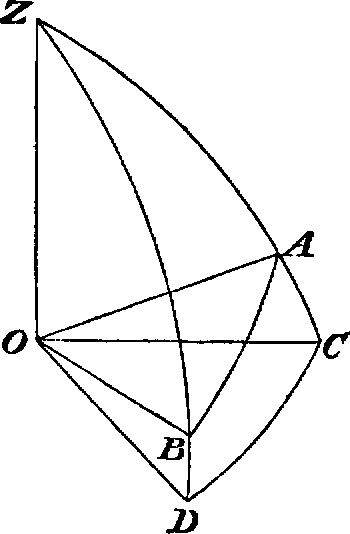
\includegraphics[width=5.0cm]{images/102fc}
\end{figure}

Suppose $OA$ and $OB$ the directions in which the two points
are seen from $O$; and let the angle $AOB$ be observed. Let $OZ$ be
the direction at right angles to the observer's horizon; describe
a sphere round $O$ as a centre, and let vertical planes through $OA$
and $OB$ meet the horizon at $OC$ and $OD$ respectively: then the
angle $COD$ is required.

Let $AOB = \theta$, $COD = \theta + x$, $AOC = h$, $BOD = k$;
from the triangle $AZB$
\[
  \cos AZB=\frac{\cos \theta-\cos ZA \,\cos ZB}{\sin ZA \,\sin ZB}=
  \frac{\cos \theta-\sin h \,\sin k}{\cos h \,\cos k}\,;
\]
and $\cos AZB=\cos COD=\cos (\theta + x)$; thus
\[
  \cos (\theta + x)=\frac{\cos \theta-\sin h \,\sin k}{\cos h \,\cos k}\,.
\]

This formula is exact; by approximation we obtain
\[
  \cos \theta-x \sin \theta=\frac{\cos \theta-hk}
{1-\frac{1}{2}(h^2+k^2)} \,;
\]
%-----File: 103.png------------------------------------------------
\begin{flalign*}
&\text{therefore }&
  x\sin \theta &= hk-\tfrac{1}{2}(h^2+k^2)\cos \theta, \text{ nearly},
&\phantom{therefore}
\\[1.5ex]
&\text{and}&
  x &= \frac{2hk - (h^2+k^2)
                   (cos^2 \tfrac{1}{2}\theta-\sin^2 \tfrac{1}{2}\theta)}
            {2 \sin \theta}
\\[1.5ex]
&&&= \tfrac{1}{4}(h + k)^2 \tan \tfrac{1}{2}\theta
   - \tfrac{1}{4}(h - k)^2 \cot \tfrac{1}{2}\theta.
\end{flalign*}

This process, by which we find the angle $COD$ from the angle
$AOB$, is called \textit{reducing an angle to the horizon}.

\chapter[On small variations in the parts of a Spherical Triangle.]{ON SMALL VARIATIONS IN THE PARTS OF A SPHERICAL TRIANGLE.}
\chaptermark{ON SMALL VARIATIONS.}

\paragraph{128.} It is sometimes important to know what amount of
error will be introduced into one of the calculated parts of a
triangle by reason of any small error which may exist in the
given parts. We will here consider an example.

\paragraph{129.} \textit{A side and the opposite angle of a spherical triangle
remain constant: determine the connexion between the small variations
of any other pair of elements}.

Suppose $C$ and $c$ to remain constant.

(1) Required the connexion between the small variations of
the other sides. We suppose $a$ and $b$ to denote the sides of one
triangle which can be formed with $C$ and $c$ as fixed elements, and
$a + \delta a$ and $b + \delta b$ to denote the sides of another such triangle;
then we require the ratio of $\delta a$ to $\delta b$ when both are extremely
small. We have
\begin{flalign*}
&& \cos c = &\cos a \,\cos b + \sin a \,\sin b \,\cos C,
\\
&\text{and}
& \cos c = &\cos (a + \delta a) \cos (b + \delta b)
 + \sin (a + \delta a) \sin (b + \delta b) \cos C;&\phantom{\text{and}}
\\
&\text{also}
&& \cos (a + \delta a) = \cos a - \sin a \,\delta a, \text{nearly},
\\
&\text{and}
&& \sin (a + \delta a) = \sin a + \cos a \,\delta a, \text{nearly},
\end{flalign*}
%-----File: 104.png------------------------------------------------
with similar formul\ae\ for $\cos (b + \delta b)$ and $\sin (b + \delta b)$. (See \textit{Plane
Trigonometry}, Chap.~\textsc{xii}.) Thus
\begin{multline*}
\cos c = (\cos a - \sin a\,\delta a) (\cos b - \sin b\,\delta b) \\
{}     + (\sin a + \cos a\,\delta a) (\sin b + \cos b\,\delta b) \cos C.
\end{multline*}

Hence by subtraction, if we neglect the product $\delta a$, $\delta b$,
\begin{multline*}
0 = \delta a (\sin a\,\cos b - \cos a\,\sin b\,\cos C) \\
{}+ \delta b (\sin b\,\cos a - \cos b\,\sin a\,\cos C);
\end{multline*}
this gives the ratio of $\delta a$ to $\delta b$ in terms of $a$, $b$, $C$. We may
express the ratio more simply in terms of $A$ and $B$; for, dividing
by $\sin a \sin b$, we get from Art.~44,
\[
  \frac{\delta a}{\sin a} \cot B\,\sin C
+ \frac{\delta b}{\sin b} \cot A\,\sin C = 0;
\]
therefore
$\hfill
\delta a \,\cos B + \delta b \,\cos A = 0.
\hfill\phantom{therefore}$

(2) Required the connexion between the small variations of
the other angles. In this case we may by means of the polar
triangle deduce from the result just found, that
\[
  \delta A \,\cos b + \delta B \,\cos a = 0;
\]
this may also be found independently as before.

(3) Required the connexion between the small variations of
a side and the opposite angle $(A,\ a)$.
\begin{flalign*}
&\text{\indent Here }&
  \sin A \sin c &= \sin C \,\sin a,
\\
&\text{and }&
  \sin (A + \delta A) \sin c &= \sin C \,\sin (a + \delta a);
\\
\intertext{hence by subtraction }
&& \cos A \,\sin c \,\delta A &= \sin C \,\cos a \,\delta a,
\\
&\text{and therefore }&
  \delta A \cot A &= \delta a \cot a.
&\phantom{and therefore }&
\end{flalign*}

(4) Required the connexion between the small variations of
a side and the adjacent angle $(a,\ B)$.
%-----File: 105.png------------------------------------------------

We have $\hfill
  \cot C \sin B = \cot c \sin a - \cos B \cos a;
\hfill\phantom{\indent We have}$\\[1ex]
proceeding as before we obtain
\[
  \cot C \cos B \delta B
= \cot c \cos a \delta a
+ \cos B \sin a \delta a
+ \cos a \sin B \delta B;
\]
therefore
\[
  (\cot C \cos B - \cos a \sin B) \delta B
= (\cot c \cos a + \cos B \sin a) \delta a;
\]
therefore $\hfill\displaystyle
-\frac{\cos A}{\sin C} \delta B = \frac{\cos b}{\sin c} \delta a;
\hfill\phantom{therefore}$\\[2ex]
therefore $\hfill\displaystyle
\delta B \cos A = - \delta a \cot b \sin B.
\hfill\phantom{therefore}$

\paragraph{130.} Some more examples are proposed for solution at the
end of this Chapter; as they involve no difficulty they are left for
the exercise of the student.

\section*{\centering\normalsize EXAMPLES.}

1. In a spherical triangle, if $C$ and $c$ remain constant while
$a$ and $b$ receive the small increments $\delta a$ and $\delta b$ respectively, shew
that
\[
  \frac{\delta a}{\surd{(1 - n^2 \sin^2 a)}} +
  \frac{\delta b}{\surd{(1 - n^2 \sin^2 b)}} = 0 \text{ where }
n = \frac{\sin C}{\sin c}\,.
\]

2. If $C$ and $c$ remain constant, and a small change be made
in $a$, find the consequent changes in the other parts of the triangle.
Find also the change in the area.
\medskip

3. Supposing $A$ and $c$ to remain constant, prove the following
equations, connecting the small variations of pairs of the other
elements:
\begin{gather*}
  \sin C \delta b =  \sin a \delta B,\quad
  \delta b \sin C = -\delta C \tan a,\quad
  \delta a \tan C =  \delta B \sin a,
\\
  \delta a \tan C = -\delta C \tan a,\quad
  \delta b \cos C =  \delta a,\quad
  \delta B \cos a = -\delta C.
\end{gather*}

4. Supposing $b$ and $c$ to remain constant, prove the following
equations connecting the small variations of pairs of the other
elements:
\begin{align*}
& \delta B \tan C =  \delta C \tan B, &
& \delta a \cot C = -\delta B \sin a,
\\
& \delta a = \delta A \sin c \sin B,  &
& \delta A \sin B \cos C = -\delta B \sin A.
\end{align*}
%-----File: 106.png------------------------------------------------

5. Supposing $B$ and $C$ to remain constant, prove the following
equations connecting the small variations of pairs of the
other elements:
\begin{align*}
  \delta b \tan c &= \delta c \tan b, &\quad
  \delta A \cot c &= \delta b \sin A,
\\
  \delta A &= \delta a \sin b \sin C, &\quad
  \delta a \sin B \cos c &= \delta b \sin A.
\end{align*}

6. If $A$ and $C$ are constant, and $b$ be increased by a small
quantity, shew that $a$ will be increased or diminished according as
$c$ is less or greater than a quadrant.

\chapter[On the connexion of Formul\ae\ in Plane and Spherical Trigonometry.]{ON THE CONNEXION OF FORMUL\AE\ IN PLANE AND SPHERICAL TRIGONOMETRY.}
\chaptermark{CONNEXION OF FORMUL\AE\ IN TRIGONOMETRY.}

\paragraph{131.} The student must have perceived that many of the
results obtained in \textit{Spherical} Trigonometry resemble others with
which he is familiar in \textit{Plane} Trigonometry. We shall now pay
some attention to this resemblance. We shall first shew how we
may deduce formul\ae\ in Plane Trigonometry from formul\ae\ in
Spherical Trigonometry; and we shall then investigate some
theorems in Spherical Trigonometry which are interesting principally
on account of their connexion with known results in Plane
Geometry and Trigonometry.

\paragraph{132.} \textit{From any formula in Spherical Trigonometry involving
the elements of a triangle, one of them being a side, it is required
to deduce the corresponding formula in Plane Trigonometry.}

Let $\alpha$, $\beta$, $\gamma$ be the lengths of the sides of the triangle, $r$ the
radius of the sphere, so that $\dfrac{\alpha}{r}$, $\dfrac{\beta}{r}$,
$\dfrac{\gamma}{r}$ are the circular measures
of the sides of the triangle; expand the functions of
$\dfrac{\alpha}{r}$, $\dfrac{\beta}{r}$, $\dfrac{\gamma}{r}$
which occur in any proposed formula in powers of
$\dfrac{\alpha}{r}$, $\dfrac{\beta}{r}$, $\dfrac{\gamma}{r}$
respectively; then if we suppose $r$ to become indefinitely great,
%-----File: 107.png------------------------------------------------
the limiting form of the proposed formula will be a relation in
Plane Trigonometry.

For example, in Art.~106, from the formula
\[
\cos A = \frac{\cos a - \cos b \cos c }{\sin b \sin c}
\]
we deduce
\[
\cos A = \frac{\beta^2 + \gamma^2 - \alpha^2}{2 \beta \gamma}
  + \frac{\alpha^4 + \beta^4 + \gamma^4 - 2 \alpha^2 \beta^2 - 2 \beta^2 \gamma^2 - 2 \gamma^2 \alpha^2}{24 \beta \gamma r^2} + \ldots;
\]
now suppose $r$ to become infinite; then ultimately
\[
\cos A = \frac{\beta^2 + \gamma^2 - \alpha^2}{2 \beta \gamma}\,;
\]
and this is the expression for the cosine of the angle of a plane
triangle in terms of the sides.

Again, in Art.~110, from the formula
\begin{flalign*}
&&& \frac{\sin A}{\sin B} = \frac{\sin a}{\sin b} &&
\\[1ex]
&\text{we deduce }&&
\frac{\sin A}{\sin B} = \frac{\alpha}{\beta} + \frac{\alpha (\beta^2 - \alpha^2)}{6 \beta r^2} + \ldots;
\\
\intertext{now suppose $r$ to become infinite; then ultimately}
&&& \frac{\sin A}{\sin B} = \frac{\alpha}{\beta},
\end{flalign*}
that is, in a plane triangle the sides are as the sines of the opposite
angles.

\paragraph{133.} \textit{To find the equation to a small circle of the sphere.}

The student can easily draw the required diagram.

Let $O$ be the pole of a small circle, $S$ a fixed point on the
sphere, $SX$ a fixed great circle of the sphere. Let $OS = \alpha$,
$OSX = \beta$; then the position of $O$ is determined by means of these
angular co-ordinates $\alpha$ and $\beta$. Let $P$ be any point on the circumference
of the small circle, $PS = \theta$, $PSX = \phi$, so that $\theta$ and $\phi$ are
%-----File: 108.png------------------------------------------------
the angular co-ordinates of $P$. Let $OP = r$. Then from the
triangle $OSP$
\[
\cos r = \cos \alpha \cos \theta + \sin \alpha \sin \theta \cos (\phi - \beta); \tag{1}
\]
this gives a relation between the angular co-ordinates of any point
on the circumference of the circle.

If the circle be a great circle then $r = \dfrac{\pi}{2}$; thus the equation
becomes
\[
0 = \cos \alpha \cos \theta + \sin \alpha \sin \theta \cos (\phi - \beta). \tag{2}
\]

It will be observed that the angular co-ordinates here used are
analogous to the \textit{latitude} and \textit{longitude} which serve to determine
the positions of places on the Earth's surface; $\theta$ is the \textit{complement
of the latitude} and $\phi$ is the \textit{longitude}.

\paragraph{134.} Equation (1) of the preceding Article may be written
thus:
\begin{multline*}
\cos r \left(\cos^2 \frac{\theta}{2} + sin^2 \frac{\theta}{2}\right)
\\
= \cos \alpha \left(\cos^2 \frac{\theta}{2}
                  - \sin^2 \frac{\theta}{2}\right)
+ 2 \sin \alpha \sin \frac{\theta}{2} \cos \frac{\theta}{2}
  \cos (\phi - \beta).
\end{multline*}

Divide by $\cos^2 \dfrac{\theta}{2}$ and rearrange; hence
\[
  \tan^2 \frac{\theta}{2} (\cos r + \cos \alpha)
- 2 \tan \frac{\theta}{2} \sin \alpha \cos (\phi - \beta)
+ \cos r - \cos \alpha = 0.
\]

Let $\tan \dfrac{\theta_1}{2}$ and $\tan \dfrac{\theta_2}{2}$ denote the values of $\tan \dfrac{\theta}{2}$ found from
this quadratic equation; then by \textit{Algebra}, Chapter \textsc{xxii.}
\[
  \tan \frac{\theta_1}{2} \tan \frac{\theta_2}{2}
= \frac{\cos r - \cos \alpha}{\cos r + \cos \alpha}
= \tan \frac{\alpha + r}{2} \tan \frac{\alpha - r}{2}.
\]

Thus the value of the product $\tan \dfrac{\theta_{1}}{2} \tan \dfrac{\theta_{2}}{2}$ is \textit{independent} of $\phi$;
this result corresponds to the well-known property of a circle in
Plane Geometry which is demonstrated in Euclid \textsc{iii.}\ 36 \textit{Corollary}.

\paragraph{135.} Let three arcs $OA$, $OB$, $OC$ meet at a point. From any
point $P$ in $OB$ draw $PM$ perpendicular to $OA$, and $PN$ perpendicular
to $OC$. The student can easily draw the required diagram.
%-----File: 109.png------------------------------------------------

Then, by Art.\ 65,
\[
\sin PM = \sin OP \sin AOB,\quad \sin PN = \sin OP \sin COB;
\]
therefore
$\hfill\displaystyle
\frac{\sin PM}{\sin PN} = \frac{\sin AOB}{\sin COB}.
\hfill\phantom{therefore}$\\

Thus the ratio of $\sin PM$ to $\sin PN$ is independent of the position
of $P$ on the arc $OB$.

\paragraph{136.} Conversely suppose that from any other point $p$ arcs $pm$
and $pn$ are drawn perpendicular to $OA$ and $OC$ respectively; then if
\[
\frac{\sin pm}{\sin pn} = \frac{\sin PM}{\sin PN},
\]
it will follow that $p$ is on the same great circle as $O$ and $P$.

\paragraph{137.} From two points $P_1$ and $P_2$ arcs are drawn perpendicular
to a fixed arc; and from a point $P$ on the same great circle
as $P_1$ and $P_2$ a perpendicular is drawn to the same fixed arc. Let
$PP_1 = \theta_1$ and $PP_2 = \theta_2$; and let the perpendiculars drawn from $P$,
$P_1$, and $P_2$ be denoted by $x$, $x_1$ and $x_2$. Then will
\[
\sin x
= \frac{\sin \theta_2}{\sin(\theta_1 + \theta_2)} \sin x_1
+ \frac{\sin \theta_1}{\sin(\theta_1 + \theta_2)} \sin x_2.
\]

Let the arc $P_1 P_2$, produced if necessary, cut the fixed arc at a
point $O$; let $\alpha$ denote the angle between the arcs. We will suppose
that $P_1$ is between $O$ and $P_2$, and that $P$ is between $P_1$ and $P_2$.

Then, by Art.~65,
\begin{align*}
\sin x_1 = \sin \alpha \sin OP_1 &= \sin \alpha \sin (OP - \theta_1) \\
    &= \sin \alpha (\sin OP \cos \theta_1 - \cos OP \sin \theta_1);\\
\sin x_2 = \sin \alpha \sin OP_2 &= \sin \alpha \sin (OP + \theta_2) \\
    &= \sin \alpha (\sin OP \cos \theta_2 + \cos OP \sin \theta_2).
\end{align*}
Multiply the former by $\sin\theta_2$, and the latter by $\sin\theta_1$, and add;
thus
\begin{align*}
\sin \theta_2 \sin x_1 + \sin \theta_1 \sin x_2 &= \sin (\theta_1 + \theta_2) \sin \alpha \sin OP\\
     &= \sin (\theta_1 + \theta_2) \sin x.
\end{align*}
%-----File: 110.png------------------------------------------------

The student should convince himself by examination that the
result holds for all relative positions of $P$, $P_1$ and $P_2$, when due
regard is paid to algebraical signs.

\paragraph{138.} The principal use of Art.\ 137 is to determine whether
three given points are on the same great circle; an illustration
will be given in Art.\ 146.

\paragraph{139.} \textit{The arcs drawn from the angles of a spherical triangle
perpendicular to the opposite sides respectively meet at a point.}
\begin{figure}[htp]
\centering
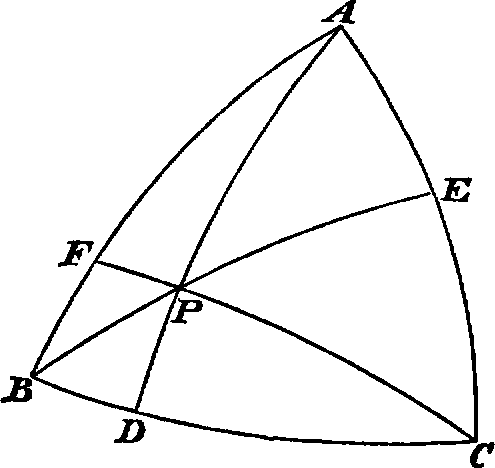
\includegraphics[width=5.0cm]{images/110fc}
\end{figure}

Let $CF$ be perpendicular to $AB$. From $F$ suppose arcs drawn
perpendicular to $CB$ and $CA$ respectively; denote the former by
$\xi$ and the latter by $\eta$. Then, by Art.\ 135,
\[
\frac{\sin\xi}{\sin\eta} = \frac{\sin FCB}{\sin FCA}.
\]

But, by Art.\ 65,
\[
  \cos B = \cos CF \sin FCB, \quad \cos A = \cos CF \sin FCA;
\]
therefore $\hfill\displaystyle
  \frac{\sin\xi}{\sin\eta}
= \frac{\cos B}{\cos A}
= \frac{\cos B \cos C}{\cos A \cos C}. \hfill\phantom{therefore}$\\[2ex]
And if from \textit{any} point in $CF$ arcs are drawn perpendicular to
$CB$ and $CA$ respectively, the ratio of the sine of the former perpendicular
to the sine of the latter perpendicular is equal to $\dfrac{\sin\xi}{\sin\eta}$
by Art.\ 135.
%-----File: 111.png------------------------------------------------

In like manner suppose $AD$ perpendicular to $BC$; then if from
any point in $AD$ arcs are drawn perpendicular to $AC$ and $AB$
respectively, the ratio of the sine of the former perpendicular to
the sine of the latter perpendicular is equal to $\dfrac{\cos A \cos C}{\cos A \cos B}$.\\[1ex]

Let $CF$ and $AD$ meet at $P$, and from $P$ let perpendiculars be
drawn on the sides $a$, $b$, $c$ of the triangle; and denote these perpendiculars
by $x$, $y$, $z$ respectively: then we have shewn that
\begin{flalign*}
&&\frac{\sin x}{\sin y} &= \frac{\cos B \cos C}{\cos A \cos C},\\[1ex]
&\text{and that}& \frac{\sin y}{\sin z} &= \frac{\cos A \cos C}{\cos A \cos B};&\phantom{and that}\\
\intertext{hence it follows that}
&&\frac{\sin x}{\sin z} &= \frac{\cos B \cos C}{\cos B \cos A},
\end{flalign*}
and this shews that the point $P$ is on the arc drawn from $B$ perpendicular
to $AC$.

Thus the three perpendiculars meet at a point, and this point
is determined by the relations
\[
\frac{\sin x}{\cos B \cos C} = \frac{\sin y}{\cos C \cos A} = \frac{\sin z}{\cos A \cos B}.
\]

\paragraph{140.} In the same manner it may be shewn that the arcs
drawn from the angles of a spherical triangle to the middle points
of the opposite sides meet at a point; and if from this point arcs
$x$, $y$, $z$ are drawn perpendicular to the sides $a$, $b$, $c$ respectively,
\[
\frac{\sin x}{\sin B \sin C} = \frac{\sin y}{\sin C \sin A} = \frac{\sin z}{\sin A \sin B}.
\]

\paragraph{141.} It is known in Plane Geometry that a certain circle
touches the inscribed and escribed circles of any triangle; this
circle is called the \textit{Nine points circle}: see \textit{Appendix to Euclid},
pages 317, 318, and \textit{Plane Trigonometry}, Chapter \textsc{xxiv}.
%-----File: 112.png------------------------------------------------

We shall now shew that a small circle can always be determined
on the sphere to touch the inscribed and escribed circles of
any spherical triangle.

\paragraph{142.} Let $\alpha$ denote the distance from $A$ of the pole of the
small circle inscribed within a spherical triangle $ABC$. Suppose
that a small circle of angular radius $\rho$ touches this inscribed circle
internally; let $\beta$ be the distance from $A$ of the pole of this touching
circle; let $\gamma$ be the angle between arcs drawn from $A$ to the
pole of the inscribed circle and the pole of the touching circle
respectively. Then we must have
\[
\cos(\rho-r) = \cos\alpha\cos\beta + \sin\alpha\sin\beta\cos\gamma. \tag{1}
\]
Suppose that this touching circle also touches externally the
escribed circle of angular radius $r_1$; then if $\alpha_1$ denote the distance
from $A$ of the pole of this escribed circle, we must have
\[
\cos(\rho+r_1) = \cos\alpha_1\cos\beta + \sin\alpha_1\sin\beta\cos\gamma. \tag{2}
\]

Similarly, if $\alpha_2$ and $\alpha_3$ denote the distances from $A$ of the poles
of the other escribed circles, in order that the touching circle may
touch these escribed circles externally, we must also have
\begin{gather*}
\cos(\rho+r_2) = \cos\alpha_2\cos\beta + \sin\alpha_2\sin\beta \cos\left(\frac{\pi}{2}-\gamma\right), \tag{3}\\[1.5ex]
\cos(\rho+r_3) = \cos\alpha_3\cos\beta + \sin\alpha_3\sin\beta \cos\left(\frac{\pi}{2}+\gamma\right). \tag{4}
\end{gather*}

We shall shew that real values of $\rho$, $\beta$, and $\gamma$ can be found to
satisfy these four equations.

Eliminate $\cos \gamma$ from (1) and (2); thus
\begin{multline*}
\cos\rho(\cos r\sin\alpha_1-\cos r_1\sin\alpha) +
\sin\rho(\sin r\sin\alpha_1+\sin r_1\sin\alpha) \\
= \cos\beta (\cos\alpha \sin\alpha_1 - \cos\alpha_1 \sin\alpha). \tag{5}
\end{multline*}

Suppose that the inscribed circle touches $AB$ at the distance $m$
from $A$, and that the escribed circle of angular radius $r_1$ touches
$AB$ at the distance $m_1$ from $A$. Then, by Art.~65,
%-----File: 113.png------------------------------------------------
\[
  \cot \alpha = \cot m \cos \frac{A}{2}, \quad
  \cos \alpha = \cos r\cos m, \quad
  \sin r = \sin \alpha \sin\frac{A}{2};
\]
therefore $\hfill\displaystyle
  \frac{\cos r}{\sin \alpha}
= \frac{\cot \alpha}{\cos m} =
\frac{1}{\sin m}\cos\frac{A}{2}.
\hfill\phantom{therefore }$\\

Similarly we may connect $\alpha_1$ and $r_1$ with $m_1$. Thus we
obtain from (5)
\begin{multline*}
\cos\rho \cos\frac{A}{2}
\left(\frac{1}{\sin m}-\frac{1}{\sin m_1}\right) +
2\sin\rho\sin\frac{A}{2}
\\
= \cos\beta\cos\frac{A}{2}
\left(\cot m-\cot m_1\right);
\end{multline*}
therefore \ $
   \cos\rho(\sin m_1-\sin m)
+ 2\sin\rho\sin m\sin m_1\tan\dfrac{A}{2} \hfill$ \\
\rightline{$ = \cos\beta\sin(m_1-m)$.}

But by Arts.~89 and 90 we have $m = s-a$, and $m_1 = s$; therefore
by the aid of Art.~45 we obtain
\[
\tag{6}
2\cos\rho=sin\frac{a}{2}\cos\frac{b+c}{2} +
2n\sin\rho=\cos\beta\sin a ,
\]
where $n$ has the meaning assigned in Art.~46.

In like manner if we eliminate $\sin \gamma$ between (3) and (4),
putting $m_2$ for $s-c$, and $m_3$ for $s-b$, we obtain
\begin{multline*}
  \cos\rho(\sin m_2+\sin m_3)
-2\sin\rho\sin m_2\sin m_3\cot\frac{A}{2}
\\
=\cos\beta\sin(m_2+m_3),
\end{multline*}
\begin{flalign*}
\tag{7}
\text{therefore}\quad&
2\cos\rho\sin\frac{a}{2}\cos\frac{b-c}{2}-2n\sin\rho=\cos\beta\sin a. &&
\end{flalign*}

From (6) and (7) we get
\[
\tag{8}
\tan\rho=
\frac{\sin\dfrac{a}{2}\sin\dfrac{b}{2}\sin\dfrac{c}{2}}{n} =
\frac{1}{2}\tan R,\ \text{by Art.~92}
\]
and $\hfill
\cos\beta=
\dfrac{\cos\dfrac{b}{2}\cos\dfrac{c}{2}\cos\rho}{\cos\dfrac{a}{2}}. \hfill\phantom{and } (9)$\\[2ex]
%-----File: 114.png------------------------------------------------

We may suppose that $\cos\dfrac{a}{2}$ is not less than $\cos\dfrac{b}{2}$ or $\cos\dfrac{c}{2}$, so
that we are sure of a possible value of $\cos\beta$ from (9).

It remains to shew that when $\rho$ and $\beta$ are thus determined, all
the four fundamental equations are satisfied.

It will be observed that, $\rho$ and $\beta$ being considered known,
$\cos\gamma$ can be found from (1) or (2), and $\sin\gamma$ can be found from
(3) or (4): we must therefore shew that (1) and (2) give the
\textit{same} value for $\cos\gamma$, and that (3) and (4) give the \textit{same} value
for $\sin\gamma$; and we must also shew that these values satisfy the
condition $\cos^2\gamma+\sin^2\gamma=1$.

From (1) we have
\[
\frac{\cos\rho\sin r}{\sin\alpha}\left(\cot r+\tan\rho-\cos m\cot r\frac{\cos\beta}{\cos\rho}\right)=\sin\beta\cos\gamma,
\]
that is,
\begin{gather*}
\frac{\cos\rho\sin\dfrac{A}{2}}{n}
 \left\{\sin s+\sin\tfrac12a\sin\tfrac12b\sin\tfrac12c
  - \frac{\cos(s-a)\sin s\cos\dfrac{b}{2}\cos\dfrac{c}{2}}{\cos\dfrac{a}{2}}\right\}\\
=\sin\beta\cos\gamma;\\
\intertext{this reduces to}
\frac{\cos\rho\sin\dfrac{A}{2}}{n}
 \left\{\cos\frac{a}{2}\sin\frac{b+c}{2}
  - \frac{\sin(b+c)\cos\dfrac{b}{2}\cos\dfrac{c}{2}}{2\cos\dfrac{a}{2}} \right\}
  =\sin\beta\cos\gamma:
\end{gather*}
and it will be found that (2) reduces to the same; so that (1) and
(2) give the same value for $\cos\gamma$.

In like manner it will be found that (3) and (4) agree in
reducing to
\[
\frac{\cos\rho\cos\dfrac{A}{2}}{n}
 \left\{\cos\dfrac{a}{2}\sin\frac{c-b}{2}
  - \frac{\sin(c-b)\cos\dfrac{b}{2}\cos\dfrac{c}{2}}{2\cos\dfrac{a}{2}} \right\}
  =\sin\beta\cos\gamma.
\]
%-----File: 115.png------------------------------------------------

It only remains to shew that the condition $\cos^2\gamma+\sin^2\gamma=1$ is
satisfied.
\[
\text{Put $k$ for $\frac{\cos\beta}{\cos\rho}$, that is for $\frac{\cos\dfrac b2 \cos\dfrac c2}{\cos\dfrac a2}$;}
\]
put $X$ for $\cot r\{1-k\cos(s-a)\}$, and $Y$ for $\cot r_1\{1-k\cos s\}$.

Then (1) and (2) may be written respectively thus:
\begin{align*}
(X\cos\rho+\sin\rho)\sin\frac A2 &=\sin\beta\cos\gamma,\tag{10}\\
(Y\cos\rho-\sin\rho)\sin\frac A2 &=\sin\beta\cos\gamma.\tag{11}
\end{align*}
From (10) and (11) by addition
\begin{flalign*}
&&\multispan{2}{\hfil$(X+Y)\sin\dfrac A2\cos\rho = 2\sin\beta\cos\gamma$;\hfil}&&\\
&\text{therefore}&
  4\sin^2\beta\cos^2\gamma&=(X^2+Y^2+2XY)\sin^2\frac A2\cos^2\rho.
&\phantom{therefore}\tag{12}
\end{flalign*}

But from (10) and (11) by subtraction
\begin{flalign*}
&&\multispan{2}{\hfil$(X-Y)\cos\rho=-2\sin\rho$;\hfil}&&\\
&\text{therefore}&
  (X^2+Y^2)\cos^2\rho&=4\sin^2\rho+2XY\cos^2\rho.&\phantom{therefore}
\end{flalign*}

Substitute in (12) and we obtain
\[
\sin^2\beta\cos^2\gamma=(\sin^2\rho+XY\cos^2\rho)\sin^2\frac A2.\tag{13}
\]

Again, put
\[
\text{$X_1$ for $\cot r_2\{1-k\cos(s-c)\}$, and $Y_1$ for $\cot r_3\{1-k\cos(s-b)\}$.}
\]

Then (3) and (4) may be written respectively thus:
\begin{align*}
(X_1\cos\rho-\sin\rho)\cos\frac A2 &= \sin\beta\sin\gamma,\tag{14}\\
(Y_1\cos\rho-\sin\rho)\cos\frac A2 &= -\sin\beta\sin\gamma.\tag{15}
\end{align*}

From (14) and (15) by subtraction
\[
(X_1-Y_1)\cos\frac A2\cos\rho = 2\sin\beta\sin\gamma,
\]
%-----File: 116.png------------------------------------------------
and from (14) and (15) by addition,
\[
  (X_1+Y_1)\cos\rho = 2\sin\rho,
\]
whence
\[
  \sin^2 \beta \sin^2 \gamma = (\sin^2 \rho - X_1 Y_1 \cos^2\rho) \cos^2 \frac{A}{2}. \tag{16}
\]

Hence from (13) and (16) it follows that we have to establish
the relation
\[
  \sin^2 \beta = \sin^2\rho + \left( XY\sin^2\frac{A}{2} - X_1 Y_1 \cos^2 \frac{A}{2} \right) \cos^2\rho.
\]

But $\sin^2\beta = 1-\cos^2\beta = \sin^2\rho + \cos^2 \rho - k^2\cos^2\rho$,
so that the relation
reduces to
\[
  1-k^2 = XY\sin^2\frac{A}{2} - X_1 Y_1 \cos^2 \frac{A}{2}.
\]

Now
\begin{align*}
XY\sin^2\frac{A}{2}
&= \frac{\cot r \cot r_1 \{1-k\cos s\} \{1-k\cos(s-a)\} \sin(s-b)\sin(s-c)}{\sin b \sin c} \\[1.5ex]
&= \frac{\{1-k\cos s\} \{1-k\cos(s-a) \} }{\sin b \sin c }.
\end{align*}

Similarly \ $
X_1 Y_1 \cos^2 \dfrac{A}{2} = \dfrac{\{1-k\cos(s-b) \} \{1-k\cos(s-c) \} }{\sin b \sin c}$.\\[2ex]

Subtract the latter from the former; then we obtain
\begin{gather*}
\frac{k}{\sin b \sin c} \{\cos(s-b) + \cos(s-c) -\cos s -\cos(s-a) \} \\[1.5ex]
{}+ \frac{k^2}{\sin b \sin c} \{\cos s \cos(s-a) - \cos(s-b)\cos(s-c) \},
\end{gather*}
that is $\hfill
  \dfrac{2k\cos\dfrac{a}{2} }{\sin b\sin c}
  \left\{\cos\dfrac{b-c}{2} -\cos\dfrac{b+c}{2} \right\}
\hfill\phantom{that is}$\\[1ex]
\[
{}+\frac{k^2}{\sin b \sin c}
   \left\{\cos\frac{b+c+a}{2} \cos\frac{b+c-a}{2}
         - \cos\frac{a+c-b}{2} \cos\frac{a+b-c}{2} \right\}
\]
that is\hfill
$\displaystyle \dfrac{4\sin\dfrac{b}{2} \sin\dfrac{c}{2}
          \cos\dfrac{b}{2} \cos\dfrac{c}{2} }
       {\sin b \sin c}
+ \dfrac{k^2}{\sin b\sin c}
  \left\{\sin^2\dfrac{c-b}{2}
        - \sin^2\dfrac{c+b}{2} \right\},$\hfill\phantom{\text{that is}}\\[1ex]
that is $1-k^2$; which was to be shewn.
%-----File: 117.png------------------------------------------------

\paragraph{143.} Thus the existence of a circle which touches the inscribed
and escribed circles of any spherical triangle has been
established.

The distance of the pole of this touching circle from the
angles $B$ and $C$ of the triangle will of course be determined by
formul\ae\ corresponding to (9); and thus it follows that
\[
\frac{\cos\dfrac{a}{2} \cos\dfrac{c}{2} \cos\rho }{\cos\dfrac{b}{2} } \text{ and }
\frac{\cos\dfrac{a}{2} \cos\dfrac{b}{2} \cos\rho }{\cos\dfrac{c}{2} },
\]
must both be less than unity.

\paragraph{144.} Since the circle which has been determined touches
the inscribed circle internally and touches the escribed circles
externally, it is obvious that it must meet all the sides of the
spherical triangle. We will now determine the position of the
points of meeting.

Suppose the touching circle intersects the side $AB$ at points
distant $\lambda$ and $\mu$ respectively from $A$.

Then by Art.~134 we have
\[
\tan\frac{\lambda}{2} \tan\frac{\mu}{2} = \frac{\cos\rho - \cos\beta}{\cos\rho + \cos\beta}
= \frac{\cos\dfrac{a}{2} - \cos\dfrac{b}{2} \cos\dfrac{c}{2} }{\cos\dfrac{a}{2} + \cos\dfrac{b}{2} \cos\dfrac{c}{2} }. \tag{1}
\]

In the same way we must have by symmetry
\[
\tan\frac{c - \lambda}{2} \tan\frac{c - \mu}{2}
= \frac{\cos\dfrac{b}{2} - \cos\dfrac{a}{2} \cos\dfrac{c}{2} }{\cos\dfrac{b}{2} + \cos\dfrac{a}{2} \cos\dfrac{c}{2}}. \tag{2}
\]

From (2), when we substitute the value of $\tan\dfrac{\lambda}{2} \tan\dfrac{\mu}{2}$ given
by (1), we obtain
\begin{gather*}
\tan\frac{\lambda}{2} + \tan\frac{\mu}{2} =
\frac{\cos^2 \dfrac{a}{2} - \cos^2 \dfrac{b}{2} \cos^2 \dfrac{c}{2} + \cos^2 \dfrac{b}{2} \sin^2 \dfrac{c}{2} }{\cos \dfrac{b}{2} \sin \dfrac{c}{2} \left(\cos \dfrac{a}{2} + \cos \dfrac{b}{2} \cos \dfrac{c}{2}\right) }\\
%-----File: 118.png------------------------------------------------
= \frac{\cos \dfrac{a}{2} - \cos \dfrac{b}{2} \cos \dfrac{c}{2} }
       {\cos \dfrac{b}{2}   \sin \dfrac{c}{2} }
+ \frac{\cos \dfrac{b}{2}   \sin \dfrac{c}{2} }
       {\cos \dfrac{a}{2} + \cos \dfrac{b}{2} \cos \dfrac{c}{2} }. \tag{3}
\end{gather*}

From (1) and (3) we see that we may put
\begin{align*}
  \tan\frac{\lambda}{2}
&= \frac{\cos \dfrac{a}{2} - \cos \dfrac{b}{2} \cos \dfrac{c}{2} }
        {\cos \dfrac{b}{2}   \sin \dfrac{c}{2} }. \tag{4}
\\[2ex]
  \tan\frac{\mu}{2}
&= \frac{\cos \dfrac{b}{2}   \sin \dfrac{c}{2} }
        {\cos \dfrac{a}{2} + \cos \dfrac{b}{2} \cos \dfrac{c}{2} }. \tag{5}
\end{align*}

Similar formul\ae\ of course hold for the points of intersection of
the touching circle with the other sides.

\paragraph{145.} Let $z$ denote the perpendicular from the pole of the
touching circle on $AB$; then
\begin{align*}
\sin z &= \sin \beta \sin \left(\frac{A}{2} + \gamma\right) \\[1.5ex]
  &= \sin \beta \left(\sin \frac{A}{2} \cos \gamma + \cos \frac{A}{2} \sin \gamma\right).
\end{align*}

But from (2) and (3) of Art.~142 we have
\[
\sin \beta \cos \gamma = \frac{\cos \rho \sin \dfrac{A}{2} }{n}
  \left(Z - \sin \frac{a}{2} \sin \frac{b}{2} \sin \frac{c}{2} \right),
\]
where\hfill
$\displaystyle Z = \sin (s - a) - \cos s \sin (s - a) \cos \frac{b}{2} \cos \frac{c}{2} \sec \frac{a}{2},$\hfill\phantom{\text{where}}
\begin{flalign*}
&\text{and }&&
\sin \beta \sin \gamma = \frac{\cos \rho \cos \dfrac{A}{2} }{n}
  \left(Z_1 - \sin \frac{a}{2} \sin \frac{b}{2} \sin \frac{c}{2}\right),\\[2ex]
&\text{where}&&
Z_1 = \sin (s - b) - \cos (s - c) \sin (s - b) \cos \frac{b}{2} \cos \frac{c}{2} \sec \frac{a}{2}.
&\phantom{where}&
\end{flalign*}
%-----File: 119.png------------------------------------------------
Therefore
\[
\sin z = \frac{\cos \rho}{n} \left\{Z \sin^2 \frac{A}{2} +
Z_1 \cos^2 \frac{A}{2} -
\sin \frac{a}{2} \sin \frac{b}{2} \sin \frac{c}{2}\right\}.
\]

Now $Z \sin^2 \dfrac{A}{2}$
\[
= \frac{\sin (s - a) \sin (s - b) \sin (s - c)}{\sin b \sin c}
\left\{1 - \cos s \cos \frac{b}{2} \cos \frac{c}{2} \sec \frac{a}{2}\right\},
\]
and $Z_1 \cos^2 \dfrac{A}{2}$
\[
= \frac{\sin s \sin (s - a) \sin (s - b)}{\sin b \sin c}
  \left\{1 - \cos (s - c) \cos \frac{b}{2} \cos \frac{c}{2}
  \sec \frac{a}{2}\right\}.
\]

Therefore $\hfill\displaystyle
Z \sin^2 \frac{A}{2} + Z_1 \cos^2 \frac{A}{2}
\hfill\phantom{\indent Therefore}$\\[1ex]
is equal to the product of
\[
\frac{\sin (s - a) \sin (s - b)}{\sin b \sin c}
\]
into
\begin{align*}
\multispan{2}{\hfill$\displaystyle
  \sin (s - c) + \sin s - \cos \frac{b}{2} \cos \frac{c}{2} \sec \frac{a}{2}
  \left\{\sin (s - c) \cos s + \cos (s - c) \sin s
\vphantom{\frac b2} \right\} $\hfill}\\[2ex]
& = \frac{\sin (s - a) \sin (s - b)}{\sin b \sin c}
  \left\{2 \sin \frac{a + b}{2} \cos \frac{c}{2} -
  \cos \frac{b}{2} \cos \frac{c}{2} \sec \frac{a}{2} \sin (2s - c)\right\} \\[2ex]
& = \frac{\sin (s - a) \sin (s - b)}{2 \sin b \sin \dfrac{c}{2}}
  \left\{2 \sin \frac{a + b}{2} -
  \sin (a + b) \cos \frac{b}{2} \sec \frac{a}{2}\right\} \\[2ex]
& = \frac{\sin (s - a) \sin (s - b) \sin \dfrac{a + b}{2}}
  {\sin b \sin \dfrac{c}{2}}
  \left\{1 - \frac{\cos \dfrac{a + b}{2} \cos \dfrac{b}{2}}{\cos \dfrac{a}{2}}
  \right\} \\[2ex]
& = \frac{\sin (s - a) \sin (s - b) \sin^2 \dfrac{a + b}{2} \sin \dfrac{b}{2}}
  {\sin b \sin \dfrac{c}{2} \cos \dfrac{a}{2}} =
  \frac{\sin (s - a) \sin (s - b) \sin^2 \dfrac{a + b}{2}}
  {2 \cos \dfrac{a}{2} \cos \dfrac{b}{2} \sin \dfrac{c}{2}}.
\end{align*}
%-----File: 120.png------------------------------------------------

Therefore
\begin{gather*}
\sin z = \frac{\cos\rho}{n} \sin\frac{a}{2} \sin\frac{b}{2} \sin\frac{c}{2} \left\{\frac{2 \sin^2\dfrac{a + b}{2}\sin(s - a)\sin(s - b)}{\sin^2\dfrac{c}{2}\sin a\sin b}- 1\right\}\\[2ex]
= \frac{\cos\rho}{n} \sin\frac{a}{2} \sin\frac{b}{2} \sin\frac{c}{2} \left\{2 cos^2\frac{A - B}{2} - 1\right\}\text{; by (2) of Art.\ 54.}
\end{gather*}

Thus $\hfill\displaystyle
  \sin z = \frac{\cos\rho}{n} \sin\frac{a}{2} \sin\frac{b}{2} \sin\frac{c}{2} \cos(A - B) \hfill\phantom{\indent Thus}$
\[
  = \sin\rho \cos(A - B).
\]

Similar expressions hold for the perpendiculars from the pole
of the touching circle on the other sides of the spherical triangle.

\paragraph{146.} Let $P$ denote the point determined in Art.\ 139; $G$ the
point determined in Art.\ 140, and $N$ the pole of the touching
circle. We shall now shew that $P$, $G$, and $N$ are on a great
circle.

Let $x$, $y$, $z$ denote the perpendiculars from $N$ on the sides
$a$, $b$, $c$ respectively of the spherical triangle; let $x_1$, $y_1$, $z_1$ denote
the perpendiculars from $P$; and $x_2$, $y_2$, $z_2$ the perpendiculars from
$G$. Then by Arts.\ 145,
139, and 140 we have
\begin{align*}
\frac{\sin x}{\cos(B - C)} &= \frac{\sin y}{\cos(C - A)} = \frac{\sin z}{\cos(A - B)},\\[1.5ex]
\frac{\sin x_1}{\cos B \cos C} &= \frac{\sin y_1}{\cos C \cos A} = \frac{\sin z_1}{\cos A \cos B},\\[1.5ex]
\frac{\sin x_2}{\sin B \sin C} &= \frac{\sin y_2}{\sin C \sin A} = \frac{\sin z_2}{\sin A \sin B}.
\end{align*}

Hence it follows that
\begin{align*}
\sin x &= t_1 \sin x_1 + t_2 \sin x_2,\\
\sin y &= t_1 \sin y_1 + t_2 \sin y_2,\\
\sin z &= t_1 \sin z_1 + t_2 \sin z_2,
\end{align*}
%-----File: 121.png------------------------------------------------
where $t_1$ and $t_2$ are certain quantities the values of which are not
required for our purpose.

Therefore by Art.\ 137 a certain point \textit{in the same great circle}
as $P$ and $G$ is at the perpendicular distances $x$, $y$, $z$ from the sides
$a$, $b$, $c$ respectively of the spherical triangle: and hence this point
must be the point $N$.

\paragraph{147.} The resemblance of the results which have been obtained
to those which are known respecting the Nine points circle in
Plane Geometry will be easily seen.

The result $\tan\rho = \dfrac12 \tan R$ corresponds to the fact that the
radius of the Nine points circle is half the radius of the circumscribing
circle of the triangle.

From equation (4) of Art.\ 144 by supposing the radius of the
sphere to become infinite we obtain $\lambda = \dfrac{b^2 + c^2 - a^2}{2c}$: this corresponds
to the fact that the Nine points circle passes through the feet of
the perpendiculars from the angles of a triangle on the opposite
sides.

From equation (5) of Art.\ 144 by supposing the radius of the
sphere to become infinite we obtain $\mu = \dfrac{c}{2}$: this corresponds to the
fact that the Nine points circle passes through the middle points
of the sides of a triangle.

From Art.\ 145 by supposing the radius of the sphere to become
infinite we obtain $z = \dfrac12 R \cos(A - B)$: this is a known
property of the Nine points circle.

In Plane Geometry the points which correspond to the $P$, $G$,
and $N$ of Art.\ 146 are on a straight line.

\paragraph{148.} The results which have been demonstrated with respect
to the circle which touches the inscribed and escribed circles of a
spherical triangle are mainly due to Dr Hart and Dr Salmon.
See the \textit{Quarterly Journal of Mathematics}, Vol.~\textsc{vi}. page~67.
%-----File: 122.png------------------------------------------------

\section*{\centering\normalsize EXAMPLES.}

1. From the formula $\sin\dfrac{a}{2}=\Surd{\left\{\dfrac{-\cos S\cos(S-A)}{\sin B\sin C}\right\}}$ deduce the expression for the area of a plane triangle, namely
$\dfrac{a^2\sin B\sin C}{2\sin A}$, when the radius of the sphere is indefinitely increased.
\medskip

2. Two triangles $ABC$, $abc$, spherical or plane, equal in all
respects, differ slightly in position: shew that
\[
\cos ABb\cos BCc\cos CAa+\cos ACc\cos CBb\cos BAa=0.
\]

3. Deduce formul\ae\ in Plane Trigonometry from Napier's
Analogies.
\medskip

4. Deduce formul\ae\ in Plane Trigonometry from Delambre's
Analogies.
\medskip

5. From the formula
$\cos\dfrac{c}{2}\cos\dfrac{A+B}{2}
=\sin\dfrac{C}{2}\cos\dfrac{a+b}{2}$ deduce
the area of a plane triangle in terms of the sides and one of the
angles.
\medskip

6. What result is obtained from Example 7 to Chapter VI.,
by supposing the radius of the sphere infinite?
\medskip

7. From the angle $C$ of a spherical triangle a perpendicular is
drawn to the arc which joins the middle points of the sides $a$ and
$b$: shew that this perpendicular makes an angle $S-B$ with the
side $a$, and an angle $S-A$ with the side $b$.
\medskip

8. From each angle of a spherical triangle a perpendicular is
drawn to the arc which joins the middle points of the adjacent
sides. Shew that these perpendiculars meet at a point; and that
%-----File: 123.png------------------------------------------------
if $x$, $y$, $z$ are the perpendiculars from this point on the sides $a$, $b$, $c$
respectively,
\[
  \frac{\sin x}{\sin(S-B)\sin(S-C)}
= \frac{\sin y}{\sin(S-C)\sin(S-A)}
= \frac{\sin z}{\sin(S-A)\sin(S-B)}.
\]

9. Through each angle of a spherical triangle an arc is drawn
so as to make the same angle with one side which the perpendicular
on the base makes with the other side. Shew that these
arcs meet at a point; and that if $x$, $y$, $z$ are the perpendiculars
from this point on the sides $a$, $b$, $c$ respectively,
\[
\frac{\sin x}{\cos A}=\frac{\sin y}{\cos B}=\frac{\sin z}{\cos C}.
\]

10. Shew that the points determined in Examples 8 and 9,
and the point $N$ of Art.\ 146 are on a great circle.

State the corresponding theorem in Plane Geometry.
\medskip

11. If one angle of a spherical triangle remains constant while
the adjacent sides are increased, shew that the area and the sum
of the angles are increased.
\medskip

12. If the arcs bisecting two angles of a spherical triangle and
terminated at the opposite sides are equal, the bisected angles will
be equal provided their sum be less than $180^\circ$.

[Let $BOD$ and $COE$ denote these two arcs which are given
equal. If the angles $B$ and $C$ are not equal suppose $B$ the greater.
Then $CD$ is greater than $BE$ by Art.\ 58. And as the angle $OBC$
is greater than the angle $OCB$, therefore $OC$ is greater than $OB$;
therefore $OD$ is greater than $OE$. Hence the angle $ODC$ is
greater than the angle $OEB$, by Example 11. Then construct
a spherical triangle $BCF$ on the other side of $BC$, equal to $CBE$.
Since the angle $ODC$ is greater than the angle $OEB$, the angle
$FDC$ is greater than the angle $DFC$; therefore $CD$ is less than
$CF$, so that $CD$ is less than $BE$. See the corresponding problem
in Plane Geometry in the \textit{Appendix to Euclid}, page 317.]
%-----File: 124.png------------------------------------------------

\chapter[Polyhedrons.]{POLYHEDRONS.}

\paragraph{149.} A polyhedron is a solid bounded by any number of
plane rectilineal figures which are called its faces. A polyhedron
is said to be \textit{regular} when its faces are similar and equal regular
polygons, and its solid angles equal to one another.

\paragraph{150.} \textit{If $\mathrm{S}$ be the number of solid angles in any polyhedron,
$\mathrm{F}$ the number of its faces, $\mathrm{E}$ the number of its edges, then
$\mathrm{S+F=E+2}$.}

Take any point within the polyhedron as centre, and describe
a sphere of radius $r$, and draw straight lines from the centre
to each of the angular points of the polyhedron; let the points
at which these straight lines meet the surface of the sphere be
joined by arcs of great circles, so that the surface of the sphere is
divided into as many polygons as the polyhedron has faces.

Let $s$ denote the sum of the angles of any one of these polygons,
$m$ the number of its sides; then the area of the polygon is
$r^2\{s-(m-2)\pi\}$ by Art.~99. The sum of the areas of all the
polygons is the surface of the sphere, that is, $4\pi r^2$. Hence since
the number of the polygons is $F$, we obtain
\[
\textstyle
4\pi = \sum s - \pi\sum m + 2F\pi.
\]

Now $\sum s$ denotes the sum of all the angles of the polygons, and
is therefore equal to $2\pi \times$ the number of solid angles, that is, to
$2\pi S$; and $\sum m$ is equal to the number of all the sides of all the
polygons, that is, to $2E$, since every edge gives rise to an arc
which is common to two polygons. Therefore
\[
4\pi = 2\pi S-2\pi E+2F\pi;
\]
therefore $\hfill
S+F=E+2.
\hfill\phantom{therefore }$
%-----File: 125.png------------------------------------------------

\paragraph{151.} \textit{There can be only five regular polyhedrons.}

Let $m$ be the number of sides in each face of a regular polyhedron,
$n$ the number of plane angles in each solid angle; then
the entire number of plane angles is expressed by $mF$, or by $nS$,
or by $2E$; thus
\[
  mF=nS=2E, \text{ and } S+F=E+2;
\]
from these equations we obtain
\[
  S = \frac{4 m}{2(m+n)-mn}, \quad
  E = \frac{2mn}{2(m+n)-mn}, \quad
  F = \frac{4 n}{2(m+n)-mn}.
\]

These expressions must be positive integers, we must therefore
have $2(m+n)$ greater than $mn$; therefore
\[
  \frac{1}{m}+\frac{1}{n} \text{ must be greater than } \frac{1}{2};
\]
but $n$ cannot be less than 3, so that $\dfrac{1}{n}$ cannot be greater than $\dfrac{1}{3}$,
and therefore $\dfrac{1}{m}$ must be greater than $\dfrac{1}{6}$; and as $m$ must be an
integer and cannot be less than 3, the only admissible values of $m$
are 3, 4, 5. It will be found on trial that the only values of $m$
and $n$ which satisfy all the necessary conditions are the following:
each regular polyhedron derives its name from the number of its
plane faces.

\begin{center}
\begin{tabular}{|c|c|c|c|c|l|}
\hline
$m$&$n$&$S$&$E$&$F$&\multicolumn{1}{c|}{Name of regular Polyhedron.}\\[1ex]
\hline
3&3&4&6&4&Tetrahedron or regular Pyramid.\\[1ex]
4&3&8&12&6&Hexahedron or Cube.\\[1ex]
3&4&6&12&8&Octahedron.\\[1ex]
5&3&20&30&12&Dodecahedron.\\[1ex]
3&5&12&30&20&Icosahedron.\\[1ex]
\hline
\end{tabular}
\end{center}

It will be seen that the demonstration establishes something
more than the enunciation states; for it is not assumed that the
faces are equilateral and equiangular and all equal. It is in fact
%-----File: 126.png------------------------------------------------
demonstrated that, \textit{there cannot be more than five solids each of
which has all its faces with the same number of sides, and all its
solid angles formed with the same number of plane angles.}

\paragraph{152.} \textit{The sum of all the plane angles which form the solid
angles of any polyhedron is $2(S-2)\pi$.}

For if $m$ denote the number of sides in any face of the polyhedron,
the sum of the interior angles of that face is $(m-2)\pi$
by Euclid I.~32, Cor.~1. Hence the sum of all the interior angles
of all the faces is $\sum(m-2)\pi$, that is $\sum m\pi-2F\pi$, that is
$2(E-F)\pi$, that is $2(S-2)\pi$.

\paragraph{153.} \textit{To find the inclination of two adjacent faces of a regular
polyhedron.}
\begin{figure}[htp]
\centering
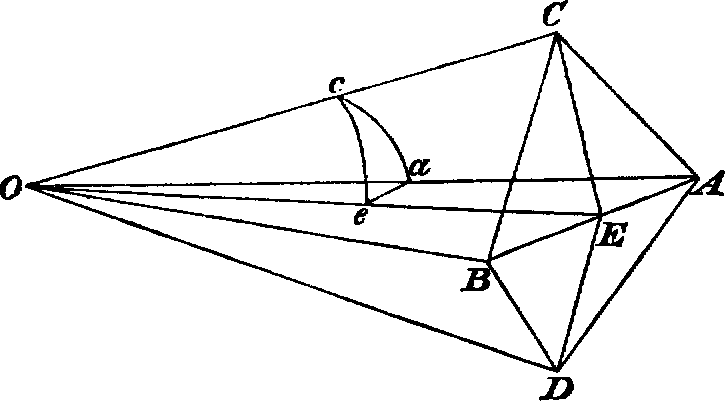
\includegraphics[width=5.0cm]{images/126fc}
\end{figure}

Let $AB$ be the edge common to the two adjacent faces, $C$ and
$D$ the centres of the faces; bisect $AB$ at $E$, and join $CE$ and $DE$;
$CE$ and $DE$ will be perpendicular to $AB$, and the angle $CED$ is
the angle of inclination of the two adjacent faces; we shall denote
it by $I$. In the plane containing $CE$ and $DE$ draw $CO$ and $DO$
at right angles to $CE$ and $DE$ respectively, and meeting at $O$;
about $O$ as centre describe a sphere meeting $OA$, $OC$, $OE$ at $a$, $c$, $e$
respectively, so that $cae$ forms a spherical triangle. Since $AB$ is
perpendicular to $CE$ and $DE$, it is perpendicular to the plane
$CED$, therefore the plane $AOB$ which contains $AB$ is perpendicular
to the plane $CED$; hence the angle $cea$ of the spherical triangle is
a right angle. Let $m$ be the number of sides in each face of the
polyhedron, $n$ the number of the plane angles which form each solid
%-----File: 127.png------------------------------------------------
angle. Then the angle $ace=ACE=\dfrac{2\pi}{2m}=\dfrac{\pi}{m}$; and the angle $cae$
is half one of the $n$ equal angles formed on the sphere round $a$,
that is, $cae=\dfrac{2\pi}{2n}=\dfrac{\pi}{n}$. From the right-angled triangle $cae$
\[
\cos{cae}=\cos{cOe}\sin{ace},
\]
\begin{flalign*}
&\text{that is }&
  \cos{\frac{\pi}{n}}
&=\cos{\left( \frac{\pi}{2} - \frac{I}{2} \right)}
  \sin{\frac{\pi}{m}}; &&
\\[1ex]
&\text{therefore }&
  \sin{\frac{I}{2}}
&=\frac{\cos \dfrac{\pi}{n}}
       {\sin{\dfrac{\pi}{m}}}. &\phantom{therefore }&
\end{flalign*}

\paragraph{154.} \textit{To find the radii of the inscribed and circumscribed
spheres of a regular polyhedron.}

Let the edge $AB=a$, let $OC=r$ and $OA=R$, so that $r$ is
the radius of the inscribed sphere, and $R$ is the radius of the
circumscribed sphere. Then
\begin{flalign*}
&& CE &= AE\cot{ACE} = \frac{a}{2}\cot{\frac{\pi}{m}}, \\[1.5ex]
&& r  &= CE\tan{CEO} = CE\tan{\frac{I}{2}}
       =\frac{a}{2}\cot{\frac{\pi}{m}}\tan{\frac{I}{2}};
\\[1.5ex]
&\text{also }&
   r  &= R\cos{aOc} = R\cot{eca}\cot{eac}
       = R\cot{\frac{\pi}{m}} \cot{\frac{\pi}{n}};
\\[1.5ex]
&\text{therefore }&
   R  &= r\tan{\frac{\pi}{m}} \tan{\frac{\pi}{n}}
       = \frac{a}{2} \tan{\frac{I}{2}} \tan{\frac{\pi}{n}}.
&\phantom{therefore }&
\end{flalign*}

\paragraph{155.} \textit{To find the surface and volume of a regular polyhedron.}

The area of one face of the polyhedron is $\dfrac{ma^2}{4}\cot{\dfrac{\pi}{m}}$, and
therefore the surface of the polyhedron is $\dfrac{mFa^2}{4}\cot{\dfrac{\pi}{m}}$.\\[.5ex]

Also the volume of the pyramid which has one face of the
polyhedron for base and $O$ for vertex is $\dfrac{r}{3}\centerdot\dfrac{ma^2}{4}\cot{\dfrac{\pi}{m}}$, and
therefore the volume of the polyhedron is $\dfrac{mFra^2}{12}\cot{\dfrac{\pi}{m}}$.\\[.5ex]
%-----File: 128.png------------------------------------------------

\paragraph{156.} \textit{To find the volume of a parallelepiped in terms of its
edges and their inclinations to one another.}
\begin{figure}[htp]
\centering
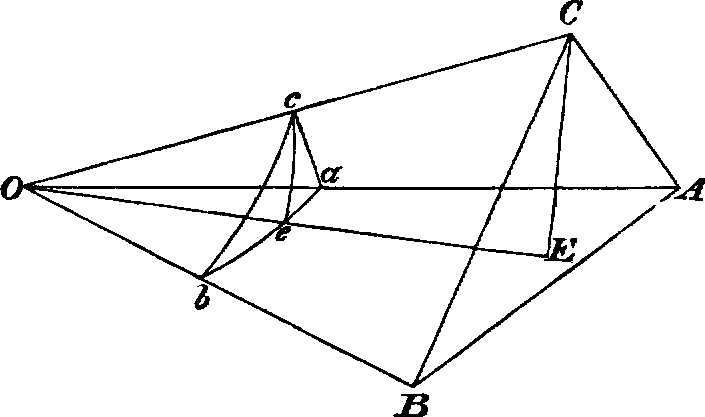
\includegraphics[width=5.0cm]{images/128fc}
\end{figure}

Let the edges be $OA=a$, $OB=b$, $OC=c$; let the inclinations
be $BOC=a$, $COA=\beta$, $AOB=\gamma$. Draw $CE$ perpendicular to the
plane $AOB$ meeting it at $E$. Describe a sphere with $O$ as a
centre, meeting $OA$, $OB$, $OC$, $OE$ at $a$, $b$, $c$, $e$ respectively.

The volume of the parallelepiped is equal to the product of its
base and altitude $=ab\sin{\gamma}\centerdot CE=abc\sin{\gamma}\sin{cOe}$. The spherical
triangle $cae$ is right-angled at $e$; thus
\[
\sin{cOe}=\sin{cOa}\sin{cae}=\sin{\beta}\sin{cab},
\]
and from the spherical triangle $cab$
\[
\sin{cab}
= \frac{\surd{( 1 - \cos^2{\alpha} - \cos^2{\beta} - \cos^2{\gamma}
              + 2\cos{\alpha}\cos{\beta}\cos{\gamma} )} }
       {\sin{\beta}\sin{\gamma} };
\]
therefore the volume of the parallelepiped
\[
= abc\surd{( 1 - \cos^2{\alpha} - \cos^2{\beta} - \cos^2{\gamma}
           + 2\cos{\alpha} \cos{\beta} \cos{\gamma} )}.
\]

\paragraph{157.} \textit{To find the diagonal of a parallelepiped in terms of the
three edges which it meets and their inclinations to one another.}

Let the edges be $OA=a$, $OB=b$, $OC=c$; let the inclinations
be $BOC=\alpha$, $COA=\beta$, $AOB=\gamma$. Let $OD$ be the diagonal required,
and let $OE$ be the diagonal of the face $OAB$. Then
\begin{align*}
OD^2 &= OE^2+ED^2+2OE\centerdot ED\cos{COE}\\
&=a^2+b^2+2ab\cos{\gamma}+c^2+2cOE\cos{COE}.
\end{align*}
%-----File: 129.png------------------------------------------------

Describe a sphere with $O$ as centre meeting $OA$, $OB$, $OC$, $OE$
at $a$, $b$, $c$, $e$ respectively; then (see Example~14, Chap.~\textsc{iv.})
\begin{figure}[htp]
\centering
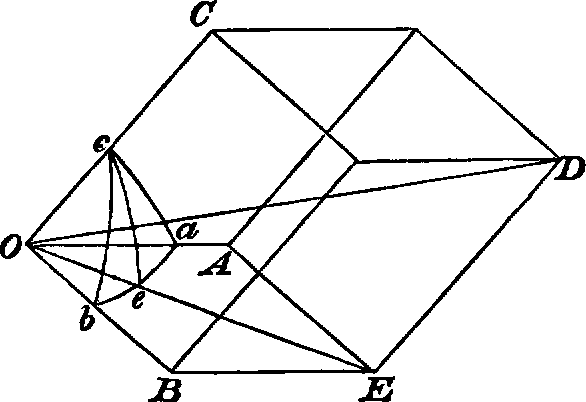
\includegraphics[width=5.0cm]{images/129fc}
\end{figure}
\begin{align*}
\cos{cOe} &= \frac{\cos{cOb}\sin{aOe}+\cos{cOa}\sin{bOe}}{\sin{aOb}}\\[1ex]
&= \frac{\cos{\alpha}\sin{aOe}+\cos{\beta}\sin{bOe}}{\sin{\gamma}};
\end{align*}
therefore\\[-1ex]
\[
  OD^2 = a^2+b^2+c^2+2ab\cos{\gamma}
       + \frac{2cOE}{\sin{\gamma}}
        (\cos{\alpha}\sin{aOe} + \cos{\beta}\sin{bOe}),
\]
\begin{flalign*}
&\text{and }&
  OE\sin{aOe} &= b\sin{\gamma}, &\qquad
  OE\sin{bOe} &= a\sin{\gamma}; &&
\\
&\text{therefore }& \multispan{4}{\hfill$
 OD^2 = a^2+b^2+c^2
       + 2ab\cos{\gamma} + 2bc\cos{\alpha} + 2ca\cos{\beta}$.
\hfill} &\phantom{therefore}&
\end{flalign*}

\paragraph{158.} \textit{To find the volume of a tetrahedron.}

A tetrahedron is one-sixth of a parallelepiped which has the
same altitude and its base double that of the tetrahedron; thus if
the edges and their inclinations are given we can take one-sixth
of the expression for the volume in Art.~156. The volume of a
tetrahedron may also be expressed in terms of its six edges; for
in the figure of Art.~156 let $BC=a'$, $CA=b'$, $AB=c'$; then
\[
  \cos{\alpha}=\frac{b^2+c^2-a'^2}{2bc}, \quad
  \cos{\beta} =\frac{c^2+a^2-b'^2}{2ca}, \quad
  \cos{\gamma}=\frac{a^2+b^2-c'^2}{2ab},
\]
and if these values are substituted for $\cos{\alpha}$, $\cos{\beta}$, and $\cos{\gamma}$ in
the expression obtained in Art.~156, the volume of the tetrahedron
will be expressed in terms of its six edges.

The following result will be obtained, in which $V$ denotes the
volume of the tetrahedron,
%-----File: 130.png------------------------------------------------
\begin{align*}
144&\hspace{3pt}V^2 = -a'^2 b'^2 c'^2\\
& + a^2a'^2 (b'^2+c'^2-a'^2)
    + b^2b'^2 (c'^2+a'^2-b'^2)
    + c^2c'^2 (a'^2+b'^2-c'^2)\\
& - a'^2 (a^2-b^2) (a^2-c^2)
    - b'^2 (b^2-c^2) (b^2-a^2)
    - c'^2 (c^2-a^2) (c^2-b^2).
\end{align*}

Thus for a \textit{regular} tetrahedron we have $144\hspace{3pt}V^2=2a^6$.

\paragraph{159.} If the vertex of a tetrahedron be supposed to be situated
at any point in the plane of its base, the volume vanishes;
hence if we equate to zero the expression on the right-hand side
of the equation just given, we obtain a relation which must hold
among the six straight lines which join four points taken arbitrarily
in a plane.

Or we may adopt Carnot's method, in which this relation is
established independently, and the expression for the volume of a
tetrahedron is deduced from it; this we shall now shew, and we
shall add some other investigations which are also given by
Carnot.

It will be convenient to alter the notation hitherto used, by
interchanging the accented and unaccented letters.

\paragraph{160.} \textit{To find the relation holding among the six straight lines
which join four points taken arbitrarily in a plane.}

Let $A$, $B$, $C$, $D$ be the four points. Let $AB=c$, $BC=a$,
$CA=b$; also let $DA=a'$, $DB=b'$, $DC=c'$.

If $D$ falls \textit{within} the triangle $ABC$, the sum of the angles
$ADB$, $BDC$, $CDA$ is equal to four right angles; so that
\[
\cos{ADB}=\cos{(BDC+CDA)}.
\]

Hence by ordinary transformations we deduce
\[
1=\cos^2{ADB}+\cos^2{BDC}+\cos^2{CDA}-2\cos{ADB}\cos{BDC}\cos{CDA}.
\]

If $D$ falls \textit{without} the triangle $ABC$, one of the three angles
at $D$ is equal to the sum of the other two, and the result just
given still holds.\\[1ex]

Now $\cos{ADB}=\dfrac{a'^2+b'^2-c^2}{2a'b'}$, and the other cosines may be
expressed in a similar manner; substitute these values in the
%-----File: 131.png------------------------------------------------
above result, and we obtain the required relation, which after
reduction may be exhibited thus,
\begin{align*}
&  0=-a^2b^2c^2\\
+ &a'^2a^2(b^2+c^2-a^2)
   + b'^2b^2(c^2+a^2-b^2)
   + c'^2c^2(a^2+b^2-c^2)\\
- &a^2(a'^2-b'^2)(a'^2-c'^2)
   - b^2(b'^2-c'^2)(b'^2-a'^2)
   - c^2(c'^2-a'^2)(c'^2-b'^2).
\end{align*}

\paragraph{161.} \textit{To express the volume of a tetrahedron in terms of its
six edges.}

Let $a$, $b$, $c$ be the lengths of the sides of a triangle $ABC$
forming one face of the tetrahedron, which we may call its base;
let $a'$, $b'$, $c'$ be the lengths of the straight lines which join $A$, $B$, $C$
respectively to the vertex of the tetrahedron. Let $p$ be the length
of the perpendicular from the vertex on the base; then the lengths
of the straight lines drawn from the foot of the perpendicular to
$A$, $B$, $C$ respectively are $\surd{(a'^2-p^2)}$, $\surd{(b'^2-p^2)}$, $\surd{(c'^2-p^2)}$. Hence
the relation given in Art.~160 will hold if we put $\surd{(a'^2-p^2)}$ instead
of $a'$, $\surd{(b'^2-p^2)}$ instead of $b'$, and $\surd{(c'^2-p^2)}$ instead of $c'$.
We shall thus obtain
\begin{align*}
&p^2(2a^2b^2+2b^2c^2+2c^2a^2 -a^4-b^4-c^4) = -a^2b^2c^2\\
& + a'^2a^2(b^2+c^2-a^2)
   + b'^2b^2(c^2+a^2-b^2)
   + c'^2c^2(a^2+b^2-c^2)\\
& - a^2(a'^2-b'^2)(a'^2-c'^2)
   - b^2(b'^2-c'^2)(b'^2-a'^2)
   - c^2(c'^2-a'^2)(c'^2-b'^2).
\end{align*}

The coefficient of $p^2$ in this equation is sixteen times the
square of the area of the triangle $ABC$; so that the left-hand
member is $144\,V^2$, where $V$ denotes the volume of the tetrahedron.
Hence the required expression is obtained.


\paragraph{162.} \textit{To find the relation holding among the six arcs of great
circles which join four points taken arbitrarily on the surface of a
sphere.}

Let $A$, $B$, $C$, $D$ be the four points. Let $AB=\gamma$, $BC=\alpha$,
$CA=\beta$; let $DA=\alpha'$, $DB=\beta'$, $DC=\gamma'$.

As in Art.\ 160 we have
\[
1=\cos^2{ADB}+\cos^2{BDC}+\cos^2{CDA}-2\cos{ADB}\cos{BDC}\cos{CDA}.
\]
%-----File: 132.png------------------------------------------------

Now $\cos{ADB}=\dfrac{\cos{\gamma}-\cos{\alpha'}\cos{\beta'}} {\sin{\alpha'}\sin{\beta}'}$, and the other cosines
may be expressed in a similar manner; substitute these values in
the above result, and we obtain the required relation, which after
reduction may be exhibited thus,
\begin{align*}
1 &= \cos^2{\alpha} +\cos^2{\beta} +\cos^2{\gamma}
   + \cos^2{\alpha'}+\cos^2{\beta'}+\cos^2{\gamma'}
\\
&{} - \cos^2{\alpha}\cos^2{\alpha'}
    - \cos^2{\beta} \cos^2{\beta'}
    - \cos^2{\gamma}\cos^2{\gamma'}
\\
&{} - 2( \cos{\alpha}\cos{\beta} \cos{\gamma}
    + \cos{\alpha}\cos{\beta'}\cos{\gamma'}
\\
&{} + \cos{\beta} \cos{\alpha'}\cos{\gamma'}
    + \cos{\gamma}\cos{\alpha'}\cos{\beta'} )
\\
&{} + 2( \cos{\alpha}\cos{\beta}\cos{\alpha'}\cos{\beta'}
    + \cos{\beta}\cos{\gamma}\cos{\beta'}\cos{\gamma'}
\\
&{} + \cos{\gamma}\cos{\alpha}\cos{\gamma'}\cos{\alpha'} ).
\end{align*}

\paragraph{163.} \textit{To find the radius of the sphere circumscribing a tetrahedron.}

Denote the edges of the tetrahedron as in Art.~161. Let the
sphere be supposed to be circumscribed about the tetrahedron,
and draw on the sphere the six arcs of great circles joining the
angular points of the tetrahedron. Then the relation given in
Art.~162 holds among the cosines of these six arcs.

Let $r$ denote the radius of the sphere. Then
\[
  \cos{\alpha}=1-2\sin^2{\frac{\alpha}{2}}
= 1-2\left( \frac{a}{2r} \right)^2 = 1 - \frac{a^2}{2r^2};
\]
and the other cosines may be expressed in a similar manner.
Substitute these values in the result of Art.~162, and we obtain,
after reduction, with the aid of Art.~161,
\begin{flalign*}
&\rlap{$4\times144\,V^2r^2=$}& \\
&&& 2a^2b^2a'^2b'^2
  + 2b^2c^2b'^2c'^2
  + 2c^2a^2c'^2a'^2 - a^4a'^4 - b^4b'^4 - c^4c'^4. &&
\end{flalign*}
The right-hand member may also be put into factors, as we see
by recollecting the mode in which the expression for the area of
a triangle is put into factors. Let $aa'+bb'+cc'=2\sigma$; then
\[
36\hspace{3pt}V^2r^2=\sigma(\sigma-aa')(\sigma-bb')(\sigma-cc').
\]
%-----File: 133.png------------------------------------------------

\section*{\centering\normalsize EXAMPLES.}

1. If $I$ denote the inclination of two adjacent faces of a
regular polyhedron, shew that $\cos I=\tfrac{1}{3}$ in the tetrahedron, $=0$
in the cube, $=-\tfrac{1}{3}$ in the octahedron, $=-\tfrac{1}{5}\surd{5}$ in the dodecahedron,
and $=-\tfrac{1}{3}\surd{5}$ in the icosahedron.
\medskip

2. With the notation of Art.\ 153, shew that the radius of
the sphere which touches one face of a regular polyhedron and all
the adjacent faces produced is $\tfrac{1}{2}a\cot{\dfrac{\pi}{m}}\cot{\tfrac{1}{2}}I$.
\medskip

3. A sphere touches one face of a regular tetrahedron and
the other three faces produced: find its radius.
\medskip

4. If $a$ and $b$ are the radii of the spheres inscribed in and
described about a regular tetrahedron, shew that $b=3a$.
\medskip

5. If $a$ is the radius of a sphere inscribed in a regular tetrahedron,
and $R$ the radius of the sphere which touches the edges,
shew that $R^2=3a^2$.
\medskip

6. If $a$ is the radius of a sphere inscribed in a regular tetrahedron,
and $R'$ the radius of the sphere which touches one face and
the others produced, shew that $R'=2a$.
\medskip

7. If a cube and an octahedron be described about a given
sphere, the sphere described about these polyhedrons will be the
same; and conversely.
\medskip

8. If a dodecahedron and an icosahedron be described about
a given sphere, the sphere described about these polyhedrons will
be the same; and conversely.
\medskip

9. A regular tetrahedron and a regular octahedron are inscribed
in the same sphere: compare the radii of the spheres
which can be inscribed in the two solids.
\medskip

10. The sum of the squares of the four diagonals of a parallelepiped
is equal to four times the sum of the squares of the
edges.
%-----File: 134.png------------------------------------------------
\medskip

11. If with all the angular points of any parallelepiped as
centres equal spheres be described, the sum of the intercepted
portions of the parallelepiped will be equal in volume to one of
the spheres.
\medskip

12. A regular octahedron is inscribed in a cube so that the
corners of the octahedron are at the centres of the faces of the
cube: shew that the volume of the cube is six times that of the
octahedron.
\medskip

13. It is not possible to fill any given space with a number
of regular polyhedrons of the same kind, except cubes; but this
may be done by means of tetrahedrons and octahedrons which
have equal faces, by using twice as many of the former as of
the latter.
\medskip

14. A spherical triangle is formed on the surface of a sphere
of radius $\rho$; its angular points are joined, forming thus a pyramid
with the straight lines joining them with the centre: shew that
the volume of the pyramid is
\[
  \tfrac{1}{3}\rho^3\surd{(\tan r\tan{r_1}\tan{r_2}\tan{r_3})},
\]
where $r$, $r_1$, $r_2$, $r_3$ are the radii of the inscribed and escribed circles
of the triangle.
\medskip

15. The angular points of a regular tetrahedron inscribed
in a sphere of radius $r$ being taken as poles, four equal small
circles of the sphere are described, so that each circle touches
the other three. Shew that the area of the surface bounded by
each circle is $2\pi r^2\left( 1 - \dfrac{1}{\surd{3}} \right)$.
\medskip

16. If $O$ be any point within a spherical triangle $ABC$, the
product of the sines of any two sides and the sine of the included
angle
\begin{multline*}
=\sin{AO}\sin{BO}\sin{CO} \biggl\{\cot{AO}\sin{BOC} \\
+\cot{BO}\sin{COA}+\cot{CO}\sin{AOB} \biggr\}.
\end{multline*}

%-----File: 135.png------------------------------------------------

\chapter[Arcs drawn to fixed points on the Surface of a Sphere.]{ARCS DRAWN TO FIXED POINTS ON THE SURFACE OF A SPHERE.}
\chaptermark{ARCS DRAWN TO FIXED POINTS.}

\paragraph{164.} In the present Chapter we shall demonstrate various
propositions relating to the arcs drawn from any point on the
surface of a sphere to certain fixed points on the surface.

\paragraph{165.} $ABC$ is a spherical triangle having all its sides quadrants,
and therefore all its angles right angles; $T$ is any point
on the surface of the sphere: to shew that
\[
\cos^2{TA}+\cos^2{TB}+\cos^2{TC}=1.
\]
\begin{figure}[htp]
\centering
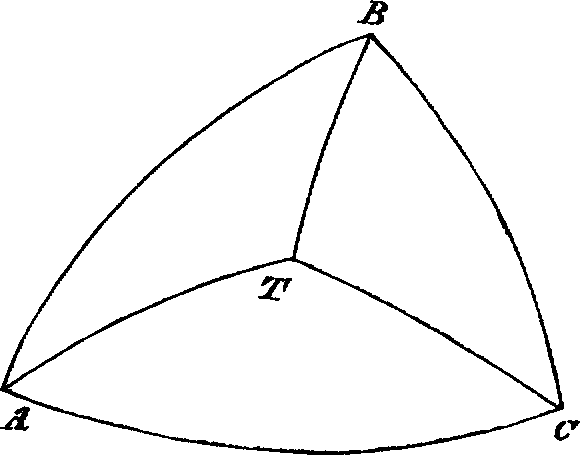
\includegraphics[width=5.0cm]{images/135fc}
\end{figure}

By Art.~37 we have
\begin{align*}
\cos{TA} &= \cos{AB}\cos{TB}+\sin{AB}\sin{TB}\cos{TBA}\\
&= \sin{TB}\cos{TBA}.
\end{align*}

Similarly\hfil
$\displaystyle \cos{TC}=\sin{TB}\cos{TBC}=\sin{TB}\sin{TBA}$.
\hfil\phantom{\indent Similarly}\\
Square and add; thus
\[
\cos^2{TA}+\cos^2{TC}=\sin^2{TB}=1-\cos^2{TB};
\]
therefore $\hfill
\cos^2{TA}+\cos^2{TB}+\cos^2{TC}=1.
\hfill\phantom{therefore }$
%-----File: 136.png------------------------------------------------

\paragraph{166.} $ABC$ is a spherical triangle having all its sides quadrants,
and therefore all its angles right angles; $T$ and $U$ are any
points on the surface of the sphere: to shew that
\[
\cos TU = \cos TA \cos UA + \cos TB \cos UB + \cos TC \cos UC.
\]
\begin{figure}[htp]
\centering
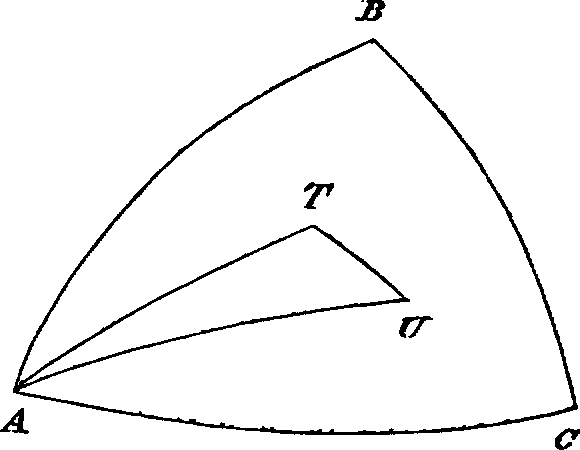
\includegraphics[width=5.0cm]{images/136fc}
\end{figure}

By Art.~37 we have
\begin{flalign*}
\multispan{6}{\hfill$
  \cos TU = \cos TA \cos UA + \sin TA \sin UA \cos TAU,$
\hfill}
\\
&\text{and }&
  \cos TAU & = \cos (BAU - BAT)                        &&\\
&&         & = \cos BAU \cos BAT + \sin BAU \sin BAT   &&\\
&&         & = \cos BAU \cos BAT + \cos CAU \cos CAT;  &&
\\
&\text{therefore }& \multispan{2}{$
  \cos TU = \cos TA \cos UA $\hfill}
&\phantom{therefore}&
\\
\multispan{4}{$\phantom{therefore}
  {}+ \sin TA \sin UA (\cos BAU \cos BAT + \cos CAU \cos CAT)
$;\hfill} &&
\end{flalign*}
\begin{flalign*}
&\text{and }&
    \cos TB & = \sin TA \cos BAT, &\phantom{and }&\\
&&  \cos UB & = \sin UA \cos BAU, &&\\
&&  \cos TC & = \sin TA \cos CAT, &&\\
&&  \cos UC & = \sin UA \cos CAU; &&
\end{flalign*}
therefore\\[-3ex]
\[
\cos TU = \cos TA \cos UA + \cos TB \cos UB + \cos TC \cos UC.
\]

\paragraph{167.} We leave to the student the exercise of shewing that
the formul\ae\ of the two preceding Articles are perfectly general for
all positions of $T$ and $U$, outside or inside the triangle $ABC$: the
%-----File: 137.png------------------------------------------------
demonstrations will remain essentially the same for all modifications
of the diagrams. The formul\ae\ are of constant application
in Analytical Geometry of three dimensions, and are demonstrated
in works on that subject; we have given them here as they may
be of service in Spherical Trigonometry, and will in fact now be
used in obtaining some important results.

\paragraph{168.} Let there be any number of fixed points on the surface
of a sphere; denote them by $H_1$, $H_2$, $H_3$,\ldots. Let $T$ be any point
on the surface of a sphere. We shall now investigate an expression
for the sum of the cosines of the arcs which join $T$ with
the fixed points.

Denote the sum by $\Sigma$; so that
\[
  \Sigma = \cos TH_1 + \cos TH_2 + \cos TH_3 + \ldots.
\]

Take on the surface of the sphere a fixed spherical triangle
$ABC$, having all its sides quadrants, and therefore all its angles
right angles.

Let $\lambda$, $\mu$, $\nu$ be the cosines of the arcs which join $T$ with
$A$, $B$, $C$ respectively; let $l_1$, $m_1$, $n_1$ be the cosines of the arcs which
join $H_1$ with $A$, $B$, $C$ respectively; and let a similar notation be
used with respect to $H_2$, $H_3$,\ldots.

Then, by Art.\ 166,
\begin{align*}
\Sigma & =l_1\lambda + m_1\mu + n_1\nu + l_2\lambda + m_2\mu + n_2\nu + \ldots\\
           & = P \lambda + Q \mu + R \nu;
\end{align*}
where $P$ stands for $l_1 + l_2 + l_3 + \ldots$, with corresponding meanings
for $Q$ and $R$.

\paragraph{169.} It will be seen that $P$ is the value which $\Sigma$ takes when
$T$ coincides with $A$, that $Q$ is the value which $\Sigma$ takes when $T$
coincides with $B$, and that $R$ is the value which $\Sigma$ takes when $T$
coincides with $C$. Hence the result expresses the general value
of $\Sigma$ in terms of the cosines of the arcs which join $T$ to the fixed
points $A$, $B$, $C$, and the particular values of $\Sigma$ which correspond
to these three points.
%-----File: 138.png------------------------------------------------

\paragraph{170.} We shall now transform the result of Art.~168.
\begin{flalign*}
&\text{\indent Let }&&
G=\surd{(P^2+Q^2+R^2)};
&\phantom{\indent Let }&
\end{flalign*}
and let $\alpha$, $\beta$, $\gamma$ be three arcs determined by the equations
\[
\cos \alpha = \frac{P}{G},\ \cos \beta \frac{Q}{G},\ \cos\gamma \frac{R}{G};
\]
then\hfill
$\Sigma=G(\lambda \cos \alpha + \mu \cos \beta + \nu \cos \gamma)$.
\hfill\phantom{\text{then}}

Since $\cos^2\alpha +\cos^2\beta+\cos^2\gamma = 1$, it is obvious that there will be
some point on the surface of the sphere, such that $\alpha$, $\beta$, $\gamma$ are the
arcs which join it to $A$, $B$, $C$ respectively; denote this point by
$U$: then, by Art.~166,
\[
\cos TU= \lambda \cos \alpha + \mu \cos \beta + \nu \cos \gamma;
\]
and finally
\[
\Sigma=G \cos TU.
\]

Thus, whatever may be the position of $T$, the sum of the cosines
of the arcs which join $T$ to the fixed points varies as the cosine
of the single arc which joins $T$ to a certain fixed point $U$.

We might take $G$ either positive or negative; it will be
convenient to suppose it positive.

\paragraph{171.} A sphere is described about a regular polyhedron;
from any point on the surface of the sphere arcs are drawn to the
solid angles of the polyhedron: to shew that the sum of the cosines
of these arcs is zero.

From the preceding Article we see that if $G$ is not zero
there is \textit{one} position of $T$ which gives to $\Sigma$ its greatest positive
value, namely, when $T$ coincides with $U$. But by the symmetry
of a regular polyhedron there must always be \textit{more than one} position
of $T$ which gives the same value to $\Sigma$. For instance, if we
take a regular tetrahedron, as there are four faces there will at
least be \textit{three other} positions of $T$ symmetrical with any assigned
position.

Hence $G$ must be zero; and thus the \textit{sum of the cosines of the
arcs which join $\mathrm{T}$ to the solid angles of the regular polyhedron is
zero for all positions of $\mathrm{T}$.}
%-----File: 139.png------------------------------------------------

\paragraph{172.} Since $G=0$, it follows that $P$, $Q$, $R$ must each be zero;
these indeed are particular cases of the general result of Art.\ 171.
See Art.\ 169.

\paragraph{173.} The result obtained in Art.\ 171 may be shewn to hold
also in some other cases. Suppose, for instance, that a rectangular
parallelepiped is inscribed in a sphere; then the sum of the
cosines of the arcs drawn from any point on the surface of the
sphere to the solid angles of the parallelepiped is zero. For here
it is obvious that there must always be at least \textit{one other} position
of $T$ symmetrical with any assigned position. Hence by the
argument of Art.\ 171 we must have $G = 0$.

\paragraph{174.} Let there be any number of fixed points on the surface
of a sphere; denote them by $H_1$, $H_2$, $H_3,\dots$ Let $T$ be any point on
the surface of the sphere. We shall now investigate a remarkable
expression for the sum of the squares of the cosines of the arcs
which join $T$ with the fixed points.

Denote the sum by $\Sigma$; so that
\[
\Sigma = \cos^2 TH_1 + \cos^2 TH_2 + \cos^2 TH_3 + \dots.
\]

Take on the surface of the sphere a fixed spherical triangle
$ABC$, having all its sides quadrants, and therefore all its angles
right angles.

Let $\lambda$, $\mu$, $\nu$ be the cosines of the arcs which join $T$ with $A$, $B$, $C$
respectively; let $l_1$, $m_1$, $n_1$ be the cosines of the angles which join
$H_1$ with $A$, $B$, $C$ respectively; and let a similar notation be used
with respect to $H_2$, $H_3$,\dots.

Then, by Art.\ 166,
\begin{gather*}
\Sigma = (l_1\lambda + m_1\mu + n_1\nu)^2 + (l_2\lambda + m_2\mu + n_2\nu)^2 + \dots.\\
\intertext{Expand each square, and rearrange the terms; thus}
\Sigma = P\lambda^2 + Q\mu^2 + R\nu^2 + 2p\mu\nu + 2q\nu\lambda + 2r\lambda \mu,\\
\text{where $P$ stands for $l_1^2 + l_2^2 + l_3^2 + \dots$,}\\
\text{and $p$ stands for $m_1n_1 + m_2n_2 + m_3n_3 + \dots$,}
\end{gather*}
with corresponding meanings for $Q$ and $q$, and for $R$ and $r$.
%-----File: 140.png------------------------------------------------

We shall now shew that there is some position of the triangle
$ABC$ for which $p$, $q$, and $r$ will vanish; so that we shall then
have
\[
\Sigma=P\lambda^2+Q\mu^2+R\nu^2.
\]

Since $\Sigma$ is always a finite positive quantity there must be some
position, or some positions, of $T$ for which $\Sigma$ has the largest value
which it can receive. Suppose that $A$ has this position, or one
of these positions if there are more than one. When $T$ is at $A$
we have $\mu$ and $\nu$ each zero, and $\lambda$ equal to unity, so that $\Sigma$ is then
equal to $P$.

Hence, whatever be the position of $T$,
$P$ is never less than $P\lambda^2+Q\mu^2+R\nu^2+2p\mu\nu+2q\nu\lambda+2r\lambda\mu$,
that is, by Art.~165,
\begin{gather*}
P(\lambda^2+\mu^2+\nu^2) \text{ is never less than}
\\
P\lambda^2+Q\mu^2+R\nu^2+2p\mu\nu+2q\nu\lambda+2r\lambda\mu;
\end{gather*}
therefore\\[-2ex]
\[
P-Q)\mu^2+(P-R)\nu^2\text{ is never less than }2p\mu\nu+2q\nu\lambda+2r\lambda\mu.
\]

Now suppose $\nu = 0$; then $T$ is situated on the great circle of
which $AB$ is a quadrant, and whatever be the position of $T$ we
have
\begin{flalign*}
&& (P-Q)\mu^2\text{ not less than } 2r\lambda\mu, &&
\\
&\text{and therefore }&
\multispan{2}{\hfill$
(P-Q\text{ not less than } \dfrac{2r\lambda}{\mu}.
$\hfill} &\phantom{and therefore }&
\end{flalign*}

But now $\dfrac{\lambda}{\mu}$ is equal to $\dfrac{\cos TA}{\cos TB}$; this is numerically equal to
$\tan TB$, and so may be made numerically as great as we please,
positive or negative, by giving a suitable position to $T$. Thus
$P-Q$ must in some cases be less than $\dfrac{2r\lambda}{\mu}$ if $r$ have any value different
from zero.

Therefore $r$ must $= 0$.

In like manner we can shew that $q$ must $= 0$.
%-----File: 141.png------------------------------------------------

Hence with the specified position for $A$ we arrive at the result
that whatever may be the position of $T$
\[
\Sigma = P\lambda^2+Q\mu^2+R\nu^2+2p\mu\,\nu.
\]

Let us now suppose that the position of $B$ is so taken that
when $T$ coincides with $B$ the value of $\Sigma$ is as large as it can be
for any point in the great circle of which $A$ is the pole. When $T$
is at $B$ we have $\lambda$ and $\nu$ each zero, and $\mu$ equal to unity, so that
$\Sigma$ is then equal to $Q$. For any point in the great circle of which
$A$ is the pole $\lambda$ is zero; and therefore for any such point
\begin{gather*}
Q \text{ is not less than }Q\mu^2+R\nu^2+2p\mu\,\nu,\\
\intertext{that is, by Art.\ 165,}
Q(\mu^2+\nu^2) \text{ is not less than }Q\mu^2+R\nu^2+2p\mu\,\nu;
\end{gather*}
therefore $Q-R$ is not less than $\dfrac{2p\mu}{\nu}$.

Hence by the same reasoning as before we must have $p = 0$.

Therefore we see that there must be some position of the
triangle $ABC$, such that for every position of $T$
\[
\Sigma = P\lambda^2+Q\mu^2+R\nu^2.
\]

\paragraph{175.} The remarks of Art.\ 169 are applicable to the result
just obtained.

\paragraph{176.} In the final result of Art.\ 174 we may shew that $R$ is
the least value which $\Sigma$ can receive. For, by Art.\ 165,
\begin{align*}
\Sigma &= P\lambda^2 + Q\mu^2 + R(1-\lambda^2-\mu^2)\\
       &= R +(P-R)\lambda^2 + (Q-R)\mu^2;
\end{align*}
and by supposition neither $P-R$ nor $Q-R$ is negative, so that
$\Sigma$ cannot be less than $R$.

\paragraph{177.} A sphere is described about a regular polyhedron; from
any point on the surface of the sphere arcs are drawn to the
solid angles of the polyhedron: it is required to find the sum of
the squares of the cosines of these arcs.
%-----File: 142.png------------------------------------------------

With the notation of Art.\ 174 we have
\[
\Sigma = P\lambda^2 + Q\mu^2 + R\nu^2.
\]

We shall shew that in the present case $P$, $Q$, and $R$ must \textit{all
be equal}. For if they are not, one of them must be greater than
each of the others, or one of them must be less than each of the
others.

If possible let the former be the case; suppose that $P$ is
greater than $Q$, and greater than $R$.
\begin{flalign*}
&\text{\indent Now }& \Sigma &= P(1 - \mu^2 - \nu^2) + Q\mu^2 + R\nu^2&\phantom{\indent Now}\\
&&& = P - (P - Q)\mu^2 - (P - R)\nu^2;
\end{flalign*}
this shews that $\Sigma$ is \textit{always less than} $P$ except when $\mu = 0$ and
$\nu = 0$: that is $\Sigma$ \textit{is always less than} $P$ except when $T$ is at $A$, or
at the point of the surface which is diametrically opposite to $A$.
But by the symmetry of a regular polyhedron there must always
be more than \textit{two} positions of $T$ which give the same value to $\Sigma$.
For instance if we take a regular tetrahedron, as there are \textit{four}
faces there will be at least \textit{three other} positions of $T$ symmetrical
with any assigned position. Hence $P$ cannot be greater than $Q$
and greater than $R$.

In the same way we can shew that one of the three $P$, $Q$,
and $R$, cannot be less than each of the others.

Therefore $P = Q = R$; and therefore by Art.\ 165 for \textit{every
position} of $T$ we have $\Sigma = P$.

Since $P = Q = R$ each of them $= \frac{1}{3}(P + Q + R)$
\begin{align*}
&= \frac13 \{{l_1}^2 + {m_1}^2 + {n_1}^2 + {l_2}^2 + {m_2}^2 + {n_2}^2 + \dots\}\\[1.5ex]
&= \frac{S}{3}, \text{ by Art.\ 165},
\end{align*}
where $S$ is the number of the solid angles of the regular polyhedron.
%-----File: 143.png------------------------------------------------

\textit{Thus the sum of the squares of the cosines of the arcs which
join any point on the surface of the sphere to the solid angles of
the regular polyhedron is one third of the number of the solid
angles.}

\paragraph{178.} Since $P=Q=R$ in the preceding Article, it will follow
that when the fixed points of Art.\ 174 are the solid angles of
a regular polyhedron, then for \textit{any} position of the spherical triangle
$ABC$ we shall have $p=0$, $q=0$, $r=0$.

For taking any position for the spherical triangle $ABC$ we
have
\[
\Sigma = P\lambda^2 + Q\mu^2 + R\nu^2 + 2p\mu\nu + 2q\nu\lambda + 2r\lambda\mu;
\]
then at $A$ we have $\mu = 0$ and $\nu = 0$, so that $P$ is then the value
of $\Sigma$; similarly $Q$ and $R$ are the values of $\Sigma$ at $B$ and $C$ respectively.
But by Art.\ 177 we have the same value for $\Sigma$ whatever
be the position of $T$; thus
\begin{flalign*}
&\phantom{therefore}&&&\phantom{therefore}&\\[-\baselineskip]
&&\multispan{2}{\hfil$P = P(\lambda^2 + \mu^2 + \nu^2) + 2p\mu\nu + 2q\nu\lambda + 2r\lambda\mu$;\hfil}&\\
&\text{therefore}&\multispan{2}{\hfil$0 = 2p\mu\nu + 2q\nu\lambda + 2r\lambda\mu$.\hfil}
\end{flalign*}

This holds then for every position of $T$. Suppose $T$ is at \textit{any
point} of the great circle of which $A$ is the pole; then $\lambda = 0$: thus
we get $p\mu\nu = 0$, and therefore $p=0$. Similarly $q=0$, and $r=0$.

\paragraph{179.} Let there be any number of fixed points on the surface
of a sphere; denote them by $H_1$, $H_2$, $H_3,\dots$; from any two points
$T$ and $U$ on the surface of the sphere arcs are drawn to the fixed
points: it is required to find the sum of the products of the corresponding
cosines, that is
\[
\cos TH_1 \cos UH_1 + \cos TH_2 \cos UH_2 + \cos TH_3 \cos UH_3 + \dots.
\]

Let the notation be the same as in Art.\ 174; and let $\lambda'$, $\mu'$, $\nu'$
be the cosines of the arcs which join $U$ with $A$, $B$, $C$ respectively.
Then by Art.\ 166,
\begin{gather*}
\cos TH_1 \cos UH_1 = (\lambda l_1 + \mu m_1 + \nu n_1)(\lambda'l_1 + \mu'm_1 + \nu'n_1) =\\
\lambda\lambda'{l_1}^2 + \mu\mu'{m_1}^2 + \nu\nu'{n_1}^2 + (\lambda\mu' + \mu\lambda')l_1m_1 + (\mu\nu' + \nu\mu')m_1n_1 + (\nu\lambda' + \lambda\nu')n_1 l_1.
\end{gather*}
%-----File: 144.png------------------------------------------------

Similar results hold for $\cos TH_2 \cos UH_2$, $\cos TH_3 \cos UH_3$,\ldots.
Hence, with the notation of Art.~174, the required sum is
\[
\lambda\lambda'P + \mu\mu'Q + \nu\nu'R + (\mu\nu' + \nu\mu')p + (\nu\lambda' + \lambda\nu')q + (\lambda\mu' + \mu\lambda')r.
\]

Now by properly choosing the position of the triangle $ABC$
we have $p$, $q$, and $r$ each zero as in Art.~174; and thus the
required sum becomes
\[
\lambda\lambda'P + \mu\mu'Q + \nu\nu'R.
\]

\paragraph{180.} The result obtained in Art.~174 may be considered
as a particular case of that just given; namely the case in which
the points $T$ and $U$ coincide.

\paragraph{181.} A sphere is described about a regular polyhedron; from
any two points on the surface of the sphere arcs are drawn to
the solid angles of the polyhedron: it is required to find the sum
of the products of the corresponding cosines.

With the notation of Art.~179 we see that the sum is
\[
\lambda\lambda'P + \mu\mu'Q + \nu\nu'R.
\]

And here $P = Q = R = \dfrac{S}{3}$, by Art.~177.

Thus the sum $= \dfrac{S}{3} (\lambda\lambda' + \mu\mu' + \nu\nu') = \dfrac{S}{3} \cos TU$.

\textit{Thus the sum of the products of the cosines is equal to the
product of the cosine $\mathrm{TU}$ into a third of the number of the solid
angles of the regular polyhedron.}

\paragraph{182.} The result obtained in Art.~177 may be considered as
a particular case of that just given; namely, the case in which
the points $T$ and $U$ coincide.

\paragraph{183.} If $TU$ is a quadrant then $\cos TU$ is zero, and the
sum of the products of the cosines in Art.~181 is zero. The
results $p = 0$, $q = 0$, $r = 0$, are easily seen to be all special examples
of this particular case.
%-----File: 145.png------------------------------------------------

\chapter[Miscellaneous Propositions.]{MISCELLANEOUS PROPOSITIONS.}

\paragraph{184.} \textit{To find the locus of the vertex of a spherical triangle of
given base and area.}

Let $AB$ be the given base, $= c$ suppose, $AC = \theta$, $BAC = \phi$.
Since the area is given the spherical excess is known; denote
it by $E$; then by Art.~103,
\begin{flalign*}
&&
  \cot \tfrac{1}{2}E
= \cot \tfrac{1}{2}\theta \cot \tfrac{1}{2}c \operatorname{cosec} \phi
+ \cot \phi; &&
\\[1.5ex]
&\text{therefore }&\multispan{2}{$\hfill
  \sin(\phi - \tfrac{1}{2}E)
= \cot \tfrac{1}{2} \theta \cot \tfrac{1}{2}c \sin \tfrac{1}{2}E;
\hfill$} &\phantom{therefore }&
\\[1.5ex]
&\text{therefore }&\multispan{2}{$\hfill
  2\cot \tfrac{1}{2}c \sin \tfrac{1}{2}E \cos^2 \dfrac{\theta}{2}
= \sin \theta \sin (\phi - \tfrac{1}{2}E);
\hfill$} &\phantom{therefore }&
\end{flalign*}
therefore
\[
  \cos \theta \cot \tfrac{1}{2}c \sin \tfrac{1}{2} E
+ \sin \theta \cos \left(\phi - \tfrac{1}{2}E + \dfrac{\pi}{2}\right)
= -\cot \tfrac{1}{2} c \sin \tfrac{1}{2} E.
\]

Comparing this with equation (1) of Art.~133, we see that the
required locus is a circle. If we call $\alpha, \beta$ the angular co-ordinates
of its pole, we have
\begin{align*}
  \tan \alpha &= \frac{1}{\cot\frac{1}{2}c\sin\frac{1}{2}E}
= \frac{\tan\frac{1}{2}c}{\sin \frac{1}{2}E} ,
\\
  \beta &= \tfrac{1}{2} E - \frac{\pi}{2}.
\end{align*}

It may be presumed from symmetry that the pole of this
circle is in the great circle which bisects $AB$ at right angles;
and this presumption is easily verified. For the equation to
that great circle is
\[
0 = \cos \theta \cos \left(\frac{\pi}{2} - \frac{c}{2}\right)
  + \sin \theta \sin \left(\frac{\pi}{2} - \frac{c}{2}\right)
    \cos (\phi - \pi)
\]
and the values $\theta = \alpha$, $\phi = \beta$ satisfy this equation.
%-----File: 146.png------------------------------------------------

\paragraph{185.} \textit{To find the angular distance between the poles of the
inscribed and circumscribed circles of a triangle.}

Let $P$ denote the pole of the inscribed circle, and $Q$ the pole
of the circumscribed circle of a triangle $ABC$; then $PAB = \frac{1}{2}A$,
by Art.\ 89, and $QAB = S-C$, by Art.\ 92; hence
\begin{gather*}
\cos PAQ = cos\tfrac{1}{2}(B-C);
\\
\text{and } \cos PQ = \cos PA \cos QA + \sin PA \sin QA \cos \tfrac{1}{2}(B-C).
\end{gather*}

Now, by Art.\ 62 (see the figure of Art.\ 89),
\begin{align*}
\cos PA &= \cos PE \cos AE = \cos r \cos(s-a), \\
\sin PA &= \frac{\sin PE}{\sin PAE} = \frac{\sin r}{\sin\tfrac{1}{2}A};
\end{align*}
thus
\[
  \cos PQ
= \cos R \cos r \cos(s-a)
+ \sin R \sin r \cos \frac{1}{2}(B-C)
 \operatorname{cosec} \tfrac{1}{2}A.
\]

Therefore, by Art.\ 54
\[
\cos PQ
= \cos R \cos r \cos(s-a)
+ \sin R \sin r \sin \tfrac{1}{2}(b+c)
 \operatorname{cosec} \tfrac{1}{2}a,
\]
\begin{flalign*}
&\text{therefore }&&
  \frac{\cos PQ}{\cos R \sin r}
= \cot r \cos(s-a)
+ \tan R \sin \frac{1}{2}(b+c) \operatorname{cosec} \frac{1}{2}a. &\phantom{therefore }&
\\[.5ex]
&\text{Now }&&
  \cot r = \frac{\sin s}{n},\quad
  \tan R = \frac{2 \sin \frac{1}{2} a \sin \tfrac{1}{2} b \sin \tfrac{1}{2} c}{n} , &&
\end{flalign*}
\begin{flalign*}
&\text{therefore }&
   \frac{\cos PQ}{\cos R \sin r}
&= \frac{1}{n}
   \Bigl\{\sin s \cos (s - a)
         + 2\sin\tfrac{1}{2}(b+c) \sin\tfrac{1}{2}b \sin\tfrac{1}{2}c \Bigr\}
&\phantom{therefore }&
\\[1ex]
&&&= \dfrac{1}{2n} (\sin a + \sin b + \sin c).
\end{flalign*}
\begin{flalign*}
&\text{Hence }&
  \left(\dfrac{\cos PQ }{\cos R \sin r}\right)^2 - 1
&= \dfrac{1}{4n^2} (\sin a + \sin b + \sin c)^2 - 1 &&
\\
&&&= (\cot r + \tan R)^2 \text{ (by Art.\ 94)}; &&
\\
&\text{therefore }&
  \cos^2 PQ &= \cos^2 R \sin^2 r + \cos^2 (R-r),
&\phantom{therefore }&
\\
&\text{and }&
  \sin^2 PQ &= \sin^2 (R-r) - \cos^2 R \sin^2 r. &&
\end{flalign*}
%-----File: 147.png------------------------------------------------

\paragraph{186.} \textit{To find the angular distance between the pole of the
circumscribed circle and the pole of one of the escribed circles of
a triangle.}

Let $Q$ denote the pole of the circumscribed circle, and $Q_1$ the
pole of the escribed circle opposite to the angle $A$. Then it may
be shewn that $QBQ_1 = \frac{1}{2} \pi + \frac{1}{2} (C-A)$, and
\begin{align*}
\cos QQ_1
&= \cos R \cos r_1 \cos (s-c)
 - \sin R \sin r_1 \sin \tfrac{1}{2}(C-A) \sec \tfrac{1}{2}B \\
&= \cos R \cos r_1 \cos (s-c)
 - \sin R \sin r_1 \sin \tfrac{1}{2}(c-a) \operatorname{cosec} \frac{1}{2}b.
\end{align*}
Therefore
\[
  \frac{\cos QQ_1}{\sin r_1 \cos R}
= \cot r_1 \cos (s - c)
- \tan R \sin \tfrac{1}{2} (c-a) \operatorname{cosec} \tfrac{1}{2} b;
\]
by reducing as in the preceding Article, the right-hand member of
the last equation becomes
\[
\dfrac{1}{2n} (\sin b + \sin c - \sin a);
\]
\begin{flalign*}
&\text{hence }&
   \left(\frac{\cos QQ_1}{\cos R \sin r_1}\right)^2 - 1
&= (\tan R - \cot r_1)^2, \text{ (Art.\ 94)};
&\phantom{therefore }&
\\
&\text{therefore }&
  \cos^2 QQ_1 &= \cos^2 R \sin^2 r_1 + \cos^2 (R + r_1), &&
\\
&\text{and }&
  \sin^2 QQ_1 &= \sin^2 (R + r_1) - \cos^2 R \sin^2 r_1.
\end{flalign*}

\paragraph{187.} \textit{The arc which passes through the middle points of the
sides of any triangle upon a given base will meet the base produced
at a fixed point, the distance of which from the middle point of the
base is a quadrant.}

Let $ABC$ be any triangle, $E$ the middle point of $AC$, and $F$
the middle point of $AB$; let the arc which joins $E$ and $F$ when
produced meet $BC$ produced at $Q$. Then
\[
  \frac{\sin BQ}{\sin BF} = \frac{\sin BFQ}{\sin BQF},\qquad
  \frac{\sin AQ}{\sin AF} = \frac{\sin AFQ}{\sin AQF};
\]
\begin{flalign*}
&\text{therefore }&&
  \frac{\sin BQ}{\sin AQ} = \frac{\sin AQF}{\sin BQF},
&\phantom{therefore }&
\end{flalign*}
%-----File: 148.png------------------------------------------------
similarly
$\hfill\displaystyle
\frac{\sin CQ}{\sin AQ} = \frac{\sin AQF}{\sin CQF};
\hfill\phantom{similarly }$\\[2ex]
therefore
$\hfill
\sin BQ = \sin CQ;\qquad \text{therefore } BQ + CQ = \pi.
\hfill\phantom{therefore }$

Hence if $D$ be the middle point of $BC$
\[
DQ = \tfrac{1}{2} (BQ + CQ) = \tfrac{1}{2} \pi.
\]

\paragraph{188.} \textit{If three arcs be drawn from the angles of a spherical
triangle through any point to meet the opposite sides, the products
of the sines of the alternate segments of the sides are equal.}
\begin{figure}[htp]
\centering
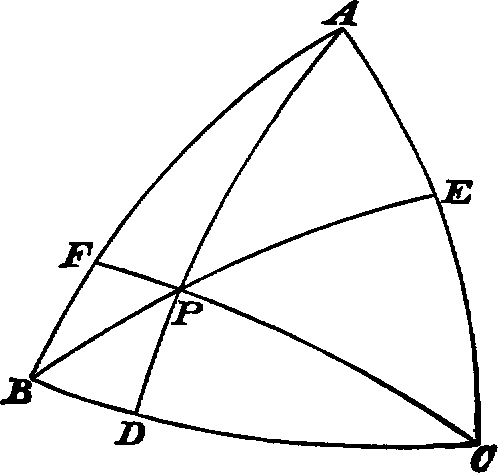
\includegraphics[width=5.0cm]{images/148fc}
\end{figure}

Let $P$ be any point, and let arcs be drawn from the angles
$A$, $B$, $C$ passing through $P$ and meeting the opposite sides at
$D$, $E$, $F$. Then
\[
  \frac{\sin BD}{\sin BP} = \frac{\sin BPD}{\sin BDP},\qquad
  \frac{\sin CD}{\sin CP} = \frac{\sin CPD}{\sin CDP},
\]
therefore
$\hfill\displaystyle
  \frac{\sin BD }{\sin CD }
= \frac{\sin BPD}{\sin CPD}\,
  \frac{\sin BP }{\sin CP }.
\hfill\phantom{therefore }$

Similar expressions may be found for $\dfrac{\sin CE}{\sin AE}$ and $\dfrac{\sin AF}{\sin BF}$;
and hence it follows obviously that
\[
  \dfrac{\sin BD}{\sin CD}\,
  \dfrac{\sin CE}{\sin AE}\,
  \dfrac{\sin AF}{\sin BF} = 1;
\]
therefore
$\hfill
\sin BD \sin CE \sin AF= \sin CD \sin AE \sin BF.
\hfill\phantom{therefore }$
%-----File: 149.png------------------------------------------------

\paragraph{189.} Conversely, when the points $D$, $E$, $F$ in the sides of a
spherical triangle are such that the relation given in the preceding
Article holds, the arcs which join these points with the opposite
angles respectively \textit{pass through a common point}. Hence the
following propositions may be established: the perpendiculars
from the angles of a spherical triangle on the opposite sides
meet at a point; the arcs which bisect the angles of a spherical
triangle meet at a point; the arcs which join the angles of a
spherical triangle with the middle points of the opposite sides
meet at a point; the arcs which join the angles of a spherical
triangle with the points where the inscribed circle touches the
opposite sides respectively meet at a point.

Another mode of establishing such propositions has been
exemplified in Arts.\ 139 and 140.

\paragraph{190.} \textit{If $\mathrm{AB}$ and $\mathrm{A'B'}$ be any two equal arcs
$\mathrm{AA'}$ and $\mathrm{AA'}$ and $\mathrm{BB'}$ be bisected at right angles by arcs meeting at $\mathrm{P}$,
then $\mathrm{AB}$ and $\mathrm{A'B'}$ subtend equal angles at $\mathrm{P}$.}
\begin{figure}[htp]
\centering
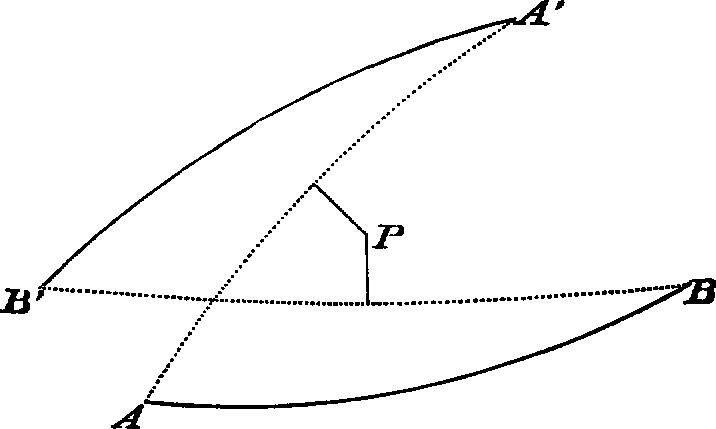
\includegraphics[width=5.0cm]{images/149fc}
\end{figure}

For $PA = PA'$ and $PB = PB'$; hence the sides of the triangle
$PAB$ are respectively equal to those of $PA'B'$; therefore the angle
$APB =$ the angle $A'PB'$.

This simple proposition has an important application to the
motion of a rigid body of which one point is fixed. For conceive
a sphere capable of motion round its centre which is fixed; then it
appears from this proposition that any two fixed points on the
%-----File: 150.png------------------------------------------------
sphere, as $A$ and $B$, can be brought into any other positions, as
$A'$ and $B'$, by rotation round an axis passing through the centre of
the sphere and a certain point $P$. Hence it may be inferred that
any change of position in a rigid body, of which one point is fixed,
may be effected by rotation round some axis through the fixed
point.
\nopagebreak\par
\rightline{(De Morgan's \textit{Differential and Integral Calculus}, page 489.)}

\paragraph{191.} Let $P$ denote any point within any \textit{plane} angle $AOB$,
and from $P$ draw perpendiculars on the straight lines $OA$ and
$OB$; then it is evident that these perpendiculars include an angle
which is the \textit{supplement} of the angle $AOB$. The corresponding
fact with respect to a \textit{solid} angle is worthy of notice. Let there
be a solid angle formed by three plane angles, meeting at a point
$O$. From any point $P$ within the solid angle, draw perpendiculars
$PL$, $PM$, $PN$ on the three planes which form the solid angle;
then the spherical triangle which corresponds to the three planes
$LPM$, $MPN$, $NPL$ is the \textit{polar triangle} of the spherical triangle
which corresponds to the solid angle at $O$. This remark is due to
Professor De Morgan.

\paragraph{192.} Suppose three straight lines to meet at a point and form
a solid angle; let $\alpha$, $\beta$, and $\gamma$ denote the angles contained by these
three straight lines taken in pairs: then it has been proposed to
call the expression $\surd(1-\cos^2 \alpha-\cos^2 \beta-\cos^2 \gamma+2\cos \alpha \cos \beta \cos \gamma)$,
the \textit{sine of the solid angle}. See Baltzer's \textit{Theorie\ldots der Determinanten},
2nd edition, page~177. Adopting this definition it is easy
to shew that the sine of a solid angle lies between zero and unity.

We know that the area of a plane triangle is half the product
of two sides into the sine of the included angle: by Art.\ 156 we
have the following analogous proposition; the volume of a tetrahedron
is one sixth of the product of three edges into the sine of
the solid angle which they form.

Again, we know in mechanics that if three forces acting at a
point are in equilibrium, each force is as the sine of the angle
between the directions of the other two: the following proposition
is analogous; if four forces acting at a point are in equilibrium
%-----File: 151.png------------------------------------------------
each force is as the sine of the solid angle formed by the directions
of the other three. See \textit{Statics}, Chapter~II\@.

\paragraph{193.} Let a sphere be described about a regular polyhedron;
let perpendiculars be drawn from the centre of the sphere on the
faces of the polyhedron, and produced to meet the surface of
the sphere: then it is obvious from symmetry that the points of
intersection must be the angular points of another regular polyhedron.

This may be verified. It will be found on examination that if
$S$ be the number of solid angles, and $F$ the number of faces of one
regular polyhedron, then another regular polyhedron exists which
has $S$ faces and $F$ solid angles. See Art.~151.

\paragraph{194.} \textit{Polyhedrons.} The result in Art.~150 was first obtained
by Euler; the demonstration which is there given is due to
Legendre. The demonstration shews that the result is true in
many cases in which the polyhedron has \textit{re-entrant} solid angles;
for all that is necessary for the demonstration is, that it shall be
possible to take a point within the polyhedron as the centre of a
sphere, so that the polygons, formed as in Art.~150, shall not have
any coincident portions. The result, however, is generally true,
even in cases in which the condition required by the demonstration
of Art.~150 is not satisfied. We shall accordingly give
another demonstration, and shall then deduce some important
consequences from the result. We begin with a theorem which
is due to Cauchy.

\paragraph{195.} \textit{Let there be any network of rectilineal figures, not necessarily
in one plane, but not forming a closed surface; let $\mathrm E$ be the
number of edges, $\mathrm F$ the number of figures, and $\mathrm S$ the number of
corner points: then $\mathrm{F + S = E + 1 }$.}

This theorem is obviously true in the case of a single plane
figure; for then $F = 1$, and $S = E$. It can be shewn to be generally
true by induction. For assume the theorem to be true for
a network of $F$ figures; and suppose that a rectilineal figure of
$n$ sides is added to this network, so that the network and the
additional figure have $m$ sides coincident, and therefore $m + 1$
%-----File: 152.png------------------------------------------------
corner points coincident. And with respect to the new network
which is thus formed, let $E'$, $F'$, $S'$ denote the same things as
$E$, $F$, $S$ with respect to the old network. Then
\[
E' = E + n-m,\quad F' = F+1,\quad S' = S + n-(m + 1);
\]
therefore
$\hfill
F' + S'- E' = F+S-E.
\hfill\phantom{therefore }$

But $F+S=E+ 1$, by hypothesis; therefore $F' + S'=E' + 1$.

\paragraph{196.} To demonstrate Euler's theorem we suppose one face of
a polyhedron removed, and we thus obtain a network of rectilineal
figures to which Cauchy's theorem is applicable. Thus
\begin{flalign*}
&                &  F-1+S &= E + 1; &&\\
&\text{therefore }& F + S &= E + 2. &\phantom{therefore }&
\end{flalign*}

\paragraph{197.} \textit{In any polyhedron the number of faces with an odd
number of sides is even, and the number of solid angles formed
with an odd number of plane angles is even.}

Let $a$, $b$, $c$, $d$,\ldots\ldots denote respectively the numbers of faces
which are triangles, quadrilaterals, pentagons, hexagons,\ldots\ldots.
Let $\alpha$, $\beta$, $\gamma$, $\delta$,\ldots\ldots denote respectively the numbers of the solid
angles which are formed with three, four, five, six,\ldots\ldots plane
angles.

Then, each edge belongs to \textit{two} faces, and terminates at \textit{two}
solid angles; therefore
\begin{align*}
  & 2E=3a+4b+5c+6d+ \ldots\ldots, \\
  & 2E= 3 \alpha + 4 \beta + 5 \gamma + 6 \delta + \ldots\ldots.
\end{align*}

From these relations it follows that $a + c + e + \ldots\ldots$, and
$\alpha + \gamma + \epsilon + \ldots\ldots$ are \textit{even} numbers.

\paragraph{198.} With the notation of the preceding Article we have
\begin{align*}
  & F=a+b+c+d+ \ldots\ldots, \\
  & S= \alpha + \beta + \gamma + \delta + \ldots\ldots.
\end{align*}

From these combined with the former relations we obtain
\begin{align*}
  & 2E-3F = b + 2c + 3d + \ldots\ldots, \\
  & 2E-3S = \beta + 2 \gamma + 3 \delta + \ldots\ldots.
\end{align*}

Thus $2E$ cannot be less than $3F$, or less than $3S$.
%-----File: 153.png------------------------------------------------

\paragraph{199.} From the expressions for $E$, $F$, and $S$, given in the
two preceding Articles, combined with the result $2F + 2S=4 + 2E$,
we obtain
\begin{gather*}
  2 (a + b + c + d + \ldots)
+ 2 (\alpha + \beta + \gamma + \delta + \ldots)
= 4 + 3a + 4b + 5c + 6d + \ldots,
\\
  2 (a + b + c + d + \ldots)
+ 2 (\alpha + \beta + \gamma + \delta + \ldots)
= 4 + 3 \alpha + 4 \beta + 5 \gamma + 6 \delta + \ldots,
\end{gather*}
therefore $\hfill
  2 (\alpha + \beta + \gamma + \delta + \ldots)
- (a + 2b + 3c + 4d + \ldots)
= 4$, \hfill(1)
\\
\phantom{therefore} $\hfill
  2 (a + b + c + d + \ldots)
- (\alpha + 2 \beta + 3 \gamma + 4 \delta + \ldots)
= 4$.\hfill(2)

Therefore, by addition
\[
a + \alpha - (c + \gamma) - 2 (d + \delta) - 3 (e + \epsilon) - \ldots\ldots = 8.
\]

\textit{Thus the number of triangular faces together with the number
of solid angles formed with three plane angles cannot be less
than eight.}

Again, from (1) and (2), by eliminating $\alpha$, we obtain
\[
3a + 2b + c - e - 2f - \ldots\ldots -2\beta - 4\gamma - \ldots\ldots = 12,
\]
so that $3a + 2b + c$ cannot be less than 12. From this result
various inferences can be drawn; thus for example, \textit{a solid cannot
be formed which shall have no triangular, quadrilateral, or pentagonal
faces.}

In like manner, we can shew that $3 \alpha + 2 \beta + \gamma$ cannot be less
than 12.

\paragraph{200.} Poinsot has shewn that in addition to the five well-known
\textit{regular polyhedrons}, four other solids exist which are
perfectly symmetrical in shape, and which might therefore also be
called \textit{regular}. We may give an idea of the nature of Poinsot's
results by referring to the case of a polygon. Suppose five points
$A$, $B$, $C$, $D$, $E$, placed in succession at equal distances round the
circumference of a circle. If we draw a straight line from each
point to the next point, we form an ordinary regular pentagon.
Suppose however we join the points by straight lines in the following
order, $A$ to $C$, $C$ to $E$, $E$ to $B$, $B$ to $D$, $D$ to $A$; we thus
form a star-shaped symmetrical figure, which might be considered
a regular pentagon.
%-----File: 154.png------------------------------------------------

It appears that, in a like manner, four, and only four, new
regular solids can be formed. To such solids, the faces of which
intersect and cross, Euler's theorem does not apply.

\paragraph{201.} Let us return to Art.~195, and suppose $e$ the number
of edges \textit{in} the bounding contour, and $e'$ the number of edges
\textit{within} it; also suppose $s$ the number of corners \textit{in} the bounding
contour, and $s'$ the number \textit{within} it. Then
\begin{flalign*}
\multispan{6}{$\hfill E = e+e'; \ S=s+s'; \hfill$} \\
&\text{therefore }& 1 + e + e' &= s + s' + F.
&\phantom{therefore }&\\[1ex]
&\text{\indent But }&       e  &= s;  &&\\
&\text{therefore }&     1 + e' &= s' + F. &&
\end{flalign*}

We can now demonstrate an extension of Euler's theorem,
which has been given by Cauchy.

\paragraph{202.} \textit{Let a polyhedron be decomposed into any number of
polyhedrons at pleasure; let $\mathrm P$ be the number thus formed, $\mathrm S$ the
number of solid angles, $\mathrm F$ the number of faces, $\mathrm E$ the number of
edges: then $\mathrm{S + F = E + P + 1 }$.}

For suppose all the polyhedrons united, by starting with one
and adding one at a time. Let $e$, $f$, $s$ be respectively the numbers
of edges, faces, and solid angles in the first; let $e'$, $f'$, $s'$ be
respectively the numbers of edges, faces, and solid angles in the
second which are not common to it and the first; let $e''$, $f''$, $s''$
be respectively the numbers of edges, faces, and solid angles in
the third which are not common to it and the first or second;
and so on. Then we have the following results, namely, the first
by Art.~196, and the others by Art.~201;
\begin{align*}
    s + f &= e + 2,\\
  s' + f' &= e' + 1,\\
s'' + f'' &= e'' + 1,\\
\multispan{2}{\dotfill}
\end{align*}

By addition, since
$s + s' + s'' + \ldots = S$,
$f + f' + f'' + \ldots = F$, and
$e + e' + e'' + \ldots = E$, we obtain
\[
  S + F = E + P + 1.
\]
%-----File: 155.png------------------------------------------------

\paragraph{203.} The following references will be useful to those who
study the theory of polyhedrons. Euler, \textit{Novi Commentarii
Acad\-emi{\ae}\ldots Pe\-tro\-pol\-i\-tan{\ae}}, Vol.~\textsc{iv.}\ 1758; Legendre, \textit{G{\'e}om{\'e}trie};
Poinsot, \textit{Journal de l'\'Ecole Polytechnique}, Cahier \textsc{x}; Cauchy,
\textit{Journal de l'\'Ecole Polytechnique}, Cahier \textsc{xvi}; Poinsot and Bertrand,
\textit{Comptes Rendus\ldots de l'Acad\-\'emie des Sciences}, Vol.~\textsc{xlvi}; Catalan,
\textit{Th{\'e}\-or\-{\`e}mes et Prob\-l{\`e}mes de G{\'e}o\-m{\'e}\-trie El\-{\'e}\-men\-taire}; Kirkman, \textit{Philosophical
Transactions} for 1856 and subsequent years; Listing,
\textit{Abhandlungen der K{\"o}nig\-lichen Ge\-sell\-schaft\ldots zu G{\"o}tt\-ingen}, Vol.~\textsc{x}.

\section*{\centering\normalsize MISCELLANEOUS EXAMPLES.}

1. Find the locus of the vertices of all right-angled spherical
triangles having the same hypotenuse; and from the equation
obtained, prove that the locus is a circle when the radius of the
sphere is infinite.
\medskip

2. $AB$ is an arc of a great circle on the surface of a sphere, $C$
its middle point: shew that the locus of the point $P$, such that
the angle $APC =$ the angle $BPC$, consists of two great circles at
right angles to one another. Explain this when the triangle
becomes plane.
\medskip

3. On a given arc of a sphere, spherical triangles of equal
area are described: shew that the locus of the angular point
opposite to the given arc is defined by the equation
\begin{multline*}
  \tan^{-1} \left\{\frac{\tan (\alpha + \phi)}{\sin \theta}\right\}
+ \tan^{-1} \left\{\frac{\tan (\alpha - \phi)}{\sin \theta}\right\} \\
{}
+ \tan^{-1} \left\{\frac{\tan \theta}{\sin (\alpha + \phi)}\right\}
+ \tan^{-1} \left\{\frac{\tan \theta}{\sin (\alpha - \phi)}\right\}
= \beta,
\end{multline*}
where $2\alpha$ is the length of the given arc, $\theta$ the arc of the great
circle drawn from any point $P$ in the locus perpendicular to the
given arc, $\phi$ the inclination of the great circle on which $\theta$ is
%-----File: 156.png------------------------------------------------
measured to the great circle bisecting the given arc at right
angles, and $\beta$ a constant.
\medskip

4. In any spherical triangle
\[
  \tan c = \frac{\cot A \cot a + \cot B \cot b}
                {\cot a \cot b - \cos A \cos B}.
\]

5. If $\theta$, $\phi$, $\psi$ denote the distances from the angles $A$, $B$, $C$
respectively of the point of intersection of arcs bisecting the
angles of the spherical triangle $ABC,$ shew that
\[
  \cos \theta \sin(b - c)
+ \cos \phi   \sin(c - a)
+ \cos \psi   \sin(a - b) = 0.
\]

6. If $A'$, $B'$, $C'$ be the poles of the sides $BC$, $CA$, $AB$ of a
spherical triangle $ABC$, shew that the great circles $AA'$, $BB'$, $CC'$
meet at a point $P$, such that
\[
  \cos PA \cos BC = \cos PB \cos CA = \cos PC \cos AB.
\]

7. If $O$ be the point of intersection of arcs $AD$, $BE$, $CF$
drawn from the angles of a triangle perpendicular to the opposite
sides and meeting them at $D$, $E$, $F$ respectively, shew that
\[
  \frac{\tan AD}{\tan OD}, \qquad
  \frac{\tan BE}{\tan OE}, \qquad
  \frac{\tan CF}{\tan OF}
\]
are respectively equal to
\[
  1+\frac{\cos A}{\cos B \cos C}, \quad
  1+\frac{\cos B}{\cos A \cos C}, \quad
  1+\frac{\cos C}{\cos A \cos B}.
\]

8. If $p$, $q$, $r$ be the arcs of great circles drawn from the
angles of a triangle perpendicular to the opposite sides, $(\alpha, \alpha')$,
$(\beta, \beta')$, $(\gamma, \gamma')$ the segments into which these arcs are divided,
shew that
\begin{flalign*}
&&&  \tan \alpha \tan \alpha'
   = \tan \beta  \tan \beta'
   = \tan \gamma \tan \gamma'; &&
\\[2ex]
&\text{and }&\multispan{2}{\hfill$\displaystyle
  \frac{\cos p}{\cos \alpha \cos \alpha'}
= \frac{\cos q}{\cos \beta  \cos \beta' }
= \frac{\cos r}{\cos \gamma \cos \gamma'}.
$\hfill} &\phantom{and }&
\end{flalign*}
%-----File: 157.png------------------------------------------------

9. In a spherical triangle if arcs be drawn from the angles to
the middle points of the opposite sides, and if $\alpha$, $\alpha'$ be the two
parts of the one which bisects the side $a$,
shew that
\[
\frac{\sin \alpha}{\sin \alpha'} = 2 \cos \frac{a}{2}.
\]

10. The arc of a great circle bisecting the sides $AB$, $AC$ of a
spherical triangle cuts $BC$ produced at $Q$: shew that
\[
\cos AQ \sin \frac{a}{2} = \sin \frac{c - b}{2} \sin \frac{c + b}{2}.
\]

11. If $ABCD$ be a spherical quadrilateral, and the opposite
sides $AB$, $CD$ when produced meet at $E$, and $AD$, $BC$ meet at $F$,
the ratio of the sines of the arcs drawn from $E$ at right angles to
the diagonals of the quadrilateral is the same as the ratio of those
from $F$.
\medskip

12. If $ABCD$ be a spherical quadrilateral whose sides $AB$,
$DC$ are produced to meet at $P$, and $AD$, $BC$ at $Q$, and whose
diagonals $AC$, $BD$ intersect at $R$, then
\[
\sin AB \sin CD \cos P = \sin AD \sin BC \cos Q = \sin AC \sin BD \cos R.
\]

13. If $A'$ be the angle of the chordal triangle which corresponds
to the angle $A$ of a spherical triangle, shew that
\[
\cos A' = \sin (S - A) \cos \frac{a}{2}.
\]

14. If the tangent of the radius of the circle described about a
spherical triangle is equal to twice the tangent of the radius of the
circle inscribed in the triangle, the triangle is equilateral.
\medskip

15. The arc $AP$ of a circle of the same radius as the sphere
is equal to the greater of two sides of a spherical triangle, and
the arc $AQ$ taken in the same direction is equal to the less; the
sine $PM$ of $AP$ is divided at $E$, so that $\dfrac{EM}{PM} =$ the natural cosine
%-----File: 158.png------------------------------------------------
of the angle included by the two sides, and $EZ$ is drawn parallel
to the tangent to the circle at $Q$. Shew that the remaining side
of the spherical triangle is equal to the arc $QPZ$.
\medskip

16. If through any point $P$ within a spherical triangle $ABC$
great circles be drawn from the angular points $A$, $B$, $C$ to meet
the opposite sides at $a$, $b$, $c$ respectively, prove that
\[
\dfrac{\sin Pa \cos PA}{\sin Aa} +
\dfrac{\sin Pb \cos PB}{\sin Bb} +
\dfrac{\sin Pc \cos PC}{\sin Cc} = 1.
\]

17. $A$ and $B$ are two places on the Earth's surface on the
same side of the equator, $A$ being further from the equator
than $B$. If the bearing of $A$ from $B$ be more nearly due East
than it is from any other place in the same latitude as $B$, find
the bearing of $B$ from $A$.
\medskip

18. From the result given in example 18 of Chapter~V.\ infer
the possibility of a regular dodecahedron.
\medskip

19. $A$ and $B$ are fixed points on the surface of a sphere, and
$P$ is any point on the surface. If $a$ and $b$ are given constants,
shew that a fixed point $S$ can always be found, in $AB$ or $AB$ produced,
such that
\[
a \cos AP + b \cos BP = s \cos SP,
\]
where $s$ is a constant.
\medskip

20. $A$, $B$, $C$,\ldots are fixed points on the surface of a sphere;
$a$, $b$, $c$,\ldots are given constants. If $P$ be a point on the surface of
the sphere, such that
\[
a \cos AP + b \cos BP + c \cos CP + \ldots = \text{constant},
\]
shew that the locus of $P$ is a circle.
%-----File: 159.png------------------------------------------------

\chapter[Numerical Solution of Spherical Triangles.]{NUMERICAL SOLUTION OF SPHERICAL TRIANGLES.}

\paragraph{204.} We shall give in this Chapter examples of the numerical
solution of Spherical Triangles.

We shall first take right-angled triangles, and then oblique-angled
triangles.

\section*{\centering\normalfont\large%
\textit{Right-Angled Triangles.}}

\paragraph{205.} Given $a = 37^\circ\, 48'\, 12''$, $b = 59^\circ\, 44'\, 16''$, $C = 90^\circ$.

To find $c$ we have
\begin{center}
$\cos c = \cos a \cos b,$\\[.1ex]
\begin{tabular}{rr@{}}
$L \cos 37^\circ\, 48'\, 12'' =$ & $9.8976927$ \\
$L \cos 59^\circ\, 44'\, 16'' =$ & $9.7023945$ \\
\cline{2-2}
$L \cos c + 10 =$ & $19.6000872$\\
$c =$ & $66^\circ\, 32'\, 6''$.
\end{tabular}
\end{center}

To find $A$ we have
\begin{center}
$\cot A = \cot a \sin b,$\\[.5ex]
\begin{tabular}{rr@{}}
$L \cot 37^\circ\, 48'\, 12'' =$ & $10.1102655$ \\
$L \sin 59^\circ\, 44'\, 16'' =$ & $ 9.9363770$ \\
\cline{2-2}
$L \cot A + 10 =$ & $ 20.0466425$\\
$A =$ & $41^\circ\, 55'\, 45''$.
\end{tabular}
\end{center}
%-----File: 160.png------------------------------------------------

To find $B$ we have
\begin{center}
$\cot B = \cot b \sin a,$\\[.1ex]
\begin{tabular}{rr@{}}
$L \cot 59^\circ\, 44'\, 16'' =$ & $ 9.7660175$\\
$L \sin 37^\circ\, 48'\, 12'' =$ & $ 9.7874272$\\
\cline{2-2}
$L \cot B + 10 = $ & $19.5534447$\\
$B =$ & $70^\circ\, 19'\, 15''$.
\end{tabular}
\end{center}

\paragraph{206.}
Given $A = 55^\circ\, 32'\, 45''$, $C = 90^\circ$, $c = 98^\circ\, 14'\, 24''$.

To find $a$ we have
\begin{center}
$\sin a = \sin c \sin A,$\\[.5ex]
\begin{tabular}{rr@{}}
$L \sin 98^\circ\, 14'\, 24'' =$ & $ 9.9954932$ \\
$L \sin 55^\circ\, 32'\, 45'' =$ & $ 9.9162323$ \\
\cline{2-2}
$L \sin a + 10                =$ & $19.9117255$ \\
$a =$ & $54^\circ\, 41'\, 35''$.
\end{tabular}
\end{center}

To find $B$ we have
\[
\cot B = \cos c \tan A.
\]

Here $\cos c$ \textit{is negative}; and therefore $\cot B$ will be negative,
and $B$ greater than a right angle. The numerical value of $\cos c$
is the same as that of $\cos 81^\circ\, 45'\, 36''$.
\begin{center}
\begin{tabular}{rr@{}}
$L \cos 81^\circ\, 45'\, 36''$ = & $ 9.1563065$ \\
$L \tan 55^\circ\, 32'\, 45''$ = & $10.1636102$ \\
\cline{2-2}
$L \cot (180^\circ - B) + 10$  = & $19.3199167$ \\
$180^\circ - B =            $    & $ 78^\circ\, 12'\, 4''$ \\
$            B =            $    & $101^\circ\, 47'\, 56''$.
\end{tabular}
\end{center}
%-----File: 161.png------------------------------------------------

To find $b$ we have
\[
\tan b = \tan c \cos A.
\]

Here $\tan c$ is \textit{negative}; and therefore $\tan b$ will be negative
and $b$ greater than a quadrant.
\begin{center}
\begin{tabular}{rr@{}}
$L \tan 81^\circ\, 45'\, 36'' =$ & $ 10.8391867 $ \\
$L \cos 55^\circ\, 32'\, 45'' =$ & $  9.7526221 $ \\
\cline{2-2}
$L \tan (180^\circ- b) + 10   =$ & $ 20.5918088 $ \\
$180^\circ - b                =$ & $ 75^\circ 38'\, 32''$ \\
$b                            =$ & $104^\circ\, 21'\, 28''$.
\end{tabular}
\end{center}

\paragraph{207.} Given $A = 46^\circ\, 15'\, 25''$, $C = 90^\circ$, $a = 42^\circ\, 18'\, 45''$.

To find $c$ we have
\begin{center}
$\sin c=\dfrac{\sin a}{\sin A},$\\[1ex]
$L \sin c = 10 + L \sin a - L \sin A,$ \\
\begin{tabular}{rr@{}}
$10 + L \sin 42^\circ\, 18'\, 45'' =$ & $19.8281272$\\
$L \sin 46^\circ\, 15'\, 25''      =$ & $ 9.8588065$\\
\cline{2-2}
$L \sin c                          =$ & $9.9693207$\\
$c = 68^\circ\, 42'\, 59'' $\text{ or }& $111^\circ\, 17'\, 1''$.
\end{tabular}
\end{center}

To find $b$ we have
\begin{center}
$\sin b = \tan a \cot A,$ \\[1ex]
\begin{tabular}{rr@{}}
$L \tan 42^\circ\, 18'\, 45'' =$ & $9.9591983$\\
$L \cot 46^\circ\, 15'\, 25'' =$ & $9.9809389$\\
\cline{2-2}
$L \sin b + 10                =$ & $19.9401372$\\
$b = 60^\circ\, 36'\, 10'' $\text{ or }& $119^\circ\, 23'\, 50''$.
\end{tabular}
\end{center}
%-----File: 162.png------------------------------------------------

To find $B$ we have
\begin{center}
$\sin B = \dfrac{\cos A}{\cos a},$\\[1ex]
$L\sin B = 10 + L\cos A - L\cos a,$\\
\begin{tabular}{rr@{}}
$10 + L\cos 46^\circ\, 15'\, 25'' =$ & $19.8397454$ \\
$L\cos 42^\circ\, 18'\, 45''      =$ & $ 9.8689289$ \\
\cline{2-2}
$L\sin B                          =$ & $ 9.9708165$ \\
$B = 69^\circ\, 13'\, 47''$\text{ or }& $ 110^\circ\, 46'\, 13''$.
\end{tabular}
\end{center}

\section*{\centering\normalfont\large%
\textit{Oblique-Angled Triangles.}}

\paragraph{208.} Given $a = 70^\circ\, 14'\, 20''$, $b = 49^\circ\, 24'\, 10''$, $c = 38^\circ\, 46'\, 10''$.
We shall use the formula given in Art.\ 45,
\[
\tan\tfrac12 A = \Surd{\left\{\frac{\sin(s - b)\sin(s - c)}{\sin s \sin(s - a)}\right\}}.
\]
\begin{flalign*}
&\text{\indent Here}& s &= 79^\circ\, 12'\, 20'',&\phantom{\indent Here}\\
&&s - a &= 8^\circ\, 58',\\
&&s - b &= 29^\circ\, 48'\, 10'',\\
&&s - c &= 40^\circ\, 26'\, 10''.
\end{flalign*}
\[
\begin{array}{r@{\:}r}
L\sin 29^\circ\, 48'\, 10'' = & \phantom{1}9.6963704\\[.3ex]
L\sin 40^\circ\, 26'\, 10''= & \phantom{1}9.8119768 \\[-1.5ex]
&\hrulefill\\[-.3ex]
  &                  19.5083472\\[1ex]
L\sin 79^\circ\, 12'\, 20''= & \phantom{1}9.9922465\\[.3ex]
L\sin 8^\circ\, 58' =& \phantom{1}9.1927342 \\[-1.5ex]
&\hrulefill\\[-.3ex]
&19.1849807\\[1ex]
&19.5083472\\[.3ex]
&19.1849807 \\[-1.5ex]
&\hrulefill\\[-.3ex]
\multicolumn{2}{r}{ 2\,\underline{)\: .3233665}} \\[.6ex]
\multicolumn{2}{r}{L\tan\tfrac12 A - 10 = \phantom{19}.1616832}
\end{array}
\]
\begin{align*}
  \tfrac12 A&= \phantom{0}55^\circ\, 25'\, 38''\\
  A &= 110^\circ\, 51'\, 16''.
\end{align*}
%-----File: 163.png------------------------------------------------

Similarly to find $B$,
\[
\begin{array}{r@{\:}r}
L \sin 8^\circ\, 58' = & \phantom{1} 9.1927342\\[.3ex]
L \sin 40^\circ\, 26'\, 10'' = & \phantom{1} 9.8119768\\[-1.5ex]
&\hrulefill\\[-.3ex]
&19.0047110\\[1ex]
L \sin 79^\circ\, 12'\, 20'' = & \phantom{1} 9.9922465\\[.3ex]
L \sin 29^\circ\, 48'\, 10'' = & \phantom{1} 9.6963704\\[-1.5ex]
&\hrulefill\\[-.3ex]
&19.6886169\\[1ex]
&19.0047110\\[.3ex]
&19.6886169\\[-1.5ex]
&\hrulefill\\[-.3ex]
\multicolumn{2}{r}{ 2\,\underline{)\: \overline{1}.3160941}}\\[.6ex]
L \tan \tfrac{1}{2}B - 10 = & \phantom{1} \overline{1}.6580470\\[.3ex]
L \tan \tfrac{1}{2}B = & \phantom{1} 9.6580470\\[.6ex]
\multispan{2}{\hfil$\begin{aligned}
\tfrac{1}{2}B &= 24^\circ\, 28'\, 2''\\
B &= 48^\circ\, 56'\, 4''.
\end{aligned}$\hfil}
\end{array}
\]
Similarly to find $C$,
\[
\begin{array}{r@{\:}r}
L \sin 8^\circ\, 58' = & \phantom{1} 9.1927342\\
L \sin 29^\circ\, 48'\, 10'' = & \phantom{1} 9.6963704\\[-1.5ex]
&\hrulefill\\[-.3ex]
&18.8891046\\[1ex]
L \sin 79^\circ\, 12'\, 20'' = & \phantom{1} 9.9922465\\[.3ex]
L \sin 40^\circ\, 26'\, 10'' = & \phantom{1} 9.8119768\\[-1.5ex]
&\hrulefill\\[-.3ex]
&19.8042233\\[1ex]
&18.8891046\\[.3ex]
&19.8042233\\[-1.5ex]
&\hrulefill\\[-.3ex]
\multicolumn{2}{r}{ 2\,\underline{)\: \overline{1}.0848813}} \\[.6ex]
L \tan \tfrac{1}{2}C-10 = & \phantom{1} \overline{1}.5424406\\[.3ex]
L \tan \tfrac{1}{2}C = & \phantom{1} 9.5424406\\[.6ex]
\multispan{2}
{\hfil$\begin{aligned}
\tfrac{1}{2}C &= 19^\circ\, 13'\, 24''\\
C &= 38^\circ\, 26'\, 48''.
\end{aligned}$\hfil}
\end{array}
\]
%-----File: 164.png------------------------------------------------

\paragraph{209.} Given
$a =  68^\circ\, 20'\, 25''$,
$b =  52^\circ\, 18'\, 15''$,
$C = 117^\circ\, 12'\, 20''$.

By Art.\ 82,
\begin{gather*}
\begin{aligned}
  \tan\tfrac12 (A + B)
&= \dfrac{\cos\tfrac12 (a - b)}{\cos\tfrac12 (a + b)}\cot\tfrac12 C,\\
  \tan\dfrac12 (A - B)
&= \dfrac{\sin\tfrac12 (a - b)}{\sin\tfrac12 (a + b)}\cot\tfrac12 C.
\end{aligned}\\
  \tfrac12(a - b) =  8^\circ\,  1'\,  5'',\
  \tfrac12(a + b) = 60^\circ\, 19'\, 20'',\
  \tfrac12C       = 58^\circ\, 36'\, 10''.
\\
\begin{array}{r@{\:}r}
  L\cos  8^\circ\,  1'\, 5''  =& \phantom{1} 9.9957335  \\[.3ex]
  L\cot 58^\circ\, 36'\, 10'' =& \phantom{1} 9.7855690  \\[-1.5ex]
&\hrulefill\\[-.3ex]
                                  &            19.7813025  \\[.6ex]
  L\cos 60^\circ\, 19'\, 20'' =& \phantom{1} 9.6947120  \\[-1.5ex]
&\hrulefill\\[-.3ex]
  L\tan\tfrac12 (A + B) =& 10.0865905  \\[.3ex]
       \tfrac12 (A + B) =&\multicolumn{1}{@{\:}l}{ 50^\circ\, 40'\, 28''}\\[1ex]
  L\sin  8^\circ\,  1'\,  5'' =& \phantom{1} 9.1445280  \\[.3ex]
  L\cot 58^\circ\, 36'\, 10'' =& \phantom{1} 9.7855690  \\[-1.5ex]
&\hrulefill\\[-.3ex]
                                  &            18.9300970  \\[.6ex]
  L\sin 60^\circ\, 19'\, 20'' =& \phantom{1} 9.9389316  \\[-1.5ex]
&\hrulefill\\[-.3ex]
  L\tan\tfrac12 (A - B) =& \phantom{1} 8.9911654\\[.3ex]
\tfrac12 (A - B) =& \multicolumn{1}{@{\:}l}{ 5^\circ\, 35'\, 47''.}
\end{array}
\end{gather*}

Therefore\quad\hfill
$A = 56^\circ\, 16'\, 15''$, \quad
$B = 45^\circ\,  4'\, 41''$. \hfill\phantom{\indent Therefore}

If we proceed to find $c$ from the formula
\[
\sin c = \dfrac{\sin a \sin C}{\sin A},
\]
since $\sin C$ is greater than $\sin A$ we shall obtain two values for $c$
both greater than $a$, and we shall not know which is the value to
be taken.
%-----File: 165.png------------------------------------------------

We shall therefore determine $c$ from formula (1) of Art.~54,
which is free from ambiguity,
\begin{gather*}
\cos \tfrac{1}{2} c = \dfrac{\cos \tfrac{1}{2} (a + b) \sin \tfrac{1}{2}C}{\cos\tfrac{1}{2}(A+B)}, \\
\begin{array}{r@{\:}r@{}c}
  L \cos 60^\circ\, 19'\, 20'' = & 9.6947120 \\[.3ex]
  L \sin 58^\circ\, 36'\, 10'' = & 9.9312422 \\[-1.5ex]
&\hrulefill\\[-.3ex]
                                 & 19.6259542 \\[.6ex]
  L \cos 50^\circ\, 40'\, 28'' = & 9.8019015 \\[-1.5ex]
&\hrulefill\\[-.3ex]
  L \cos \tfrac{1}{2} c        = & 9.8240527 \\[.3ex]
  \tfrac{1}{2} c =
&\multicolumn{2}{@{\:}l}{ 48^\circ\, 10'\, 22''} \\[.3ex]
  c =
&\multicolumn{2}{@{\:}l}{ 96^\circ\, 20'\, 44''.}
\end{array}
\end{gather*}

Or we may adopt the second method of Art.~82. First, we
determine $\theta$ from the formula $\tan \theta = \tan b \cos C$.

Here $\cos C$ \textit{is negative}, and therefore $\tan \theta$ will be negative,
and $\theta$ greater than a right angle. The numerical value of $\cos C$ is
the same as that of $\cos 62^\circ\, 47'\, 40''$.
\[
\begin{array}{r@{\:}r@{}c}
  L \tan 52^\circ\, 18'\, 15''       = & 10.1119488 \\[.3ex]
  L \cos 62^\circ\, 47'\, 40''       = &  9.6600912 \\[-1.5ex]
&\hrulefill\\[-.3ex]
  L \tan (180^\circ\, - \theta) + 10 = & 19.7720400 \\[.3ex]
  180^\circ\, - \theta =
&\multicolumn{2}{@{\:}l}{ 30^\circ\, 36'\, 33'',} \\[.3ex]
\text{therefore }\theta =
&\multicolumn{2}{@{\:}l}{ 149^\circ\, 23'\, 27''.}
\end{array}
\]

Next, we determine $c$ from the formula
\[
\cos c = \dfrac{\cos b \cos (a - \theta)}{\cos \theta}.
\]

Here $\cos \theta$ \textit{is negative}, and therefore $\cos c$ will be negative, and
$c$ will be greater than a right angle. The numerical value of
$\cos \theta$ is the same as that of $\cos (180^\circ - \theta)$, that is, of $\cos 30^\circ\, 36'\, 33''$;
and the value of $\cos (a - \theta)$ is the same as that of $\cos (\theta - a)$, that
is, of $\cos 81^\circ\, 3'\, 2''$.
%-----File: 166.png------------------------------------------------
\[
\begin{array}{r@{\:}r}
  L\cos 52^\circ\, 18'\, 15'' = & \phantom{1} 9.7863748 \\[.3ex]
  L\cos 81^\circ\,  3'\,  2'' = & \phantom{1} 9.1919060\\[-1.5ex]
&\hrulefill\\[-.3ex]
                                   &            18.9782808\\[.6ex]
  L\cos 30^\circ\, 36'\, 33'' = & \phantom{1} 9.9348319\\[-1.5ex]
&\hrulefill\\[-.3ex]
  L\cos(180^\circ - c) = & \phantom{1} 9.0434489\\[.3ex]
        180^\circ - c  =
&\multicolumn{1}{@{\:}l}{ 83^\circ\, 39'\, 17''}\\[.3ex]
  c =
&\multicolumn{1}{@{\:}l}{ 96^\circ\, 20'\, 43''.}
\end{array}
\]

Thus by taking only the nearest number of seconds in the
tables the two methods give values of $c$ which differ by $1''$; if,
however, we estimate fractions of a second both methods will
agree in giving about $43\tfrac12$ as the number of seconds.

\paragraph{210.} Given
$a = 50^\circ\, 45'\, 20''$,
$b = 69^\circ\, 12'\, 40''$,
$A = 44^\circ\, 22'\, 10''$.
\begin{flalign*}
&\text{\indent By Art.\ 84,}& \sin B &= \dfrac{\sin b}{\sin a}\sin A,&\phantom{\indent By Art.\ 84,}
\end{flalign*}
\[
\begin{array}{r@{\:}r@{}c}
\phantom{\ 4,\ or\ 122\ 25\ 8.6.}
  L\sin 69^\circ\, 12'\, 40'' = & \phantom{1} 9.9707626\\[.3ex]
  L\sin 44^\circ\, 22'\, 10'' = & \phantom{1} 9.8446525\\[-1.5ex]
&\hrulefill\\[-.3ex]
                                   &            19.8154151\\[.6ex]
  L\sin 50^\circ\, 45'\, 20'' = & \phantom{1} 9.8889956\\[-1.5ex]
&\hrulefill\\[-.3ex]
  L\sin B                        = & \phantom{1} 9.9264195\\[.3ex]
  B =
&\multicolumn{2}{@{\:}l}{ 57^\circ\, 34'\, 51''.4,\text{ or }122^\circ\, 25'\, 8''.6.}
\end{array}
\]

In this case there will be two solutions; see Art.\ 86. We
will calculate $C$ and $c$ by Napier's analogies,
\begin{align*}
\tan \tfrac12 C &= \dfrac{\cos \tfrac12 (b - a)}{\cos \tfrac12 (b + a)}\cot \tfrac12 (B + A),\\[2ex]
\tan \tfrac12 c &= \dfrac{\cos \tfrac12 (B + A)}{\cos \tfrac12 (B - A)}\tan \tfrac12 (b + a).
\end{align*}

First take the smaller value of $B$; thus
\[
  \tfrac12 (B + A) = 50^\circ\, 58'\, 30''.7,\
  \tfrac12 (B - A) =  6^\circ\, 35'\, 20''.7,
\]
%-----File: 167.png------------------------------------------------
\[
\begin{array}{r@{\:}r@{}c}
  L\cos  9^\circ\, 13'\, 40''   = & \phantom{1} 9.9943430  \\[.3ex]
  L\cot 50^\circ\, 58'\, 30''.7 = & \phantom{1} 9.9087536\\[-1.5ex]
&\hrulefill\\[-.3ex]
                                     &            19.9030966  \\[.6ex]
  L\cos 59^\circ\, 59'          = & \phantom{1} 9.6991887\\[-1.5ex]
&\hrulefill\\[-.3ex]
  L\tan\tfrac{1}{2} C                  = &            10.2039079\\[.3ex]
       \tfrac{1}{2} C                  =
&\multicolumn{2}{@{}l}{ 57^\circ\, 58'\, 55''.3}\\[.3ex]
                C                  =
&\multicolumn{2}{@{}l}{ 115^\circ\, 57'\, 50''.6.}\\[1ex]
  L\cos 50^\circ\, 58'\, 30''.7 = & \phantom{1} 9.7991039  \\[.3ex]
  L\tan 59^\circ\, 59'          = &            10.2382689\\[-1.5ex]
&\hrulefill\\[-.3ex]
                                     &            20.0373728  \\[.6ex]
  L\cos 6^\circ\, 36'\, 20''.7  = & \phantom{1} 9.9971072\\[-1.5ex]
&\hrulefill\\[-.3ex]
  L\tan\tfrac{1}{2} c                  = &            10.0402656\\[.3ex]
       \tfrac{1}{2} c                  =
&\multicolumn{2}{@{}l}{ 47^\circ\, 39'\, 8''.2}\\[.3ex]
                c                  =
&\multicolumn{2}{@{}l}{ 95^\circ\, 18'\, 16''.4.}
\end{array}
\]
Next take the larger value of $B$; thus
\begin{gather*}
  \tfrac{1}{2}(B + A) = 83^\circ\, 23'\, 39''.3,\quad
  \tfrac{1}{2}(B - A) = 39^\circ\,  1'\, 29''.3.\\
\begin{array}{r@{\:}r@{}c}
  L\cos \phantom{0}9^\circ\, 13'\, 40''\phantom{.0} =
& \phantom{1} 9.9943430\\[.3ex]
  L\cot 83^\circ\, 23'\, 39''.3 = & \phantom{1} 9.0637297\\[-1.5ex]
&\hrulefill\\[-.3ex]
                                     &            19.0580727  \\[.6ex]
  L\cos 59^\circ\, 59'          = & \phantom{1} 9.6991887\\[-1.5ex]
&\hrulefill\\[-.3ex]
  L\tan\tfrac{1}{2} C = & \phantom{1} 9.3588840\\[.3ex]
       \tfrac{1}{2} C =
&\multicolumn{2}{@{}l}{ 12^\circ\, 52'\, 15''.8}\\[.3ex]
                C =
&\multicolumn{2}{@{}l}{ 25^\circ\, 44'\, 31''.6.}\\[1ex]
  L\cos 83^\circ\, 23'\, 39''.3 = & \phantom{1} 9.0608369  \\[.3ex]
  L\tan 59^\circ\, 59'\,\phantom{00''.0} =   & 10.2382689\\[-1.5ex]
&\hrulefill\\[-.3ex]
                                                & 19.2991058  \\[.6ex]
  L\cos 39^\circ\, 1'\, 29''.3  = & \phantom{1} 9.8903494\\[-1.5ex]
&\hrulefill\\[-.3ex]
  L\tan\tfrac{1}{2} c = & \phantom{1} 9.4087564\\[.3ex]
       \tfrac{1}{2} c =
&\multicolumn{2}{@{}l}{ 14^\circ\, 22'\, 32''.6} \\[.3ex]
                c =
&\multicolumn{2}{@{}l}{ 28^\circ\, 45'\, 5''.2}
\end{array}
\end{gather*}
%-----File: 168.png------------------------------------------------

The student can obtain more examples, which can be easily
verified, from those here worked out, by interchanging the given
and required quantities, or by making use of the polar triangle.


\section*{\centering\normalsize EXAMPLES.}
\allowdisplaybreaks
\begin{flalign*}
\multispan{1}{\indent 1.\hfill\quad Given $b$}%
& = 137^\circ\, 3'\, 48'',\
A = 147^\circ\, 2'\, 54'',\
C =  90^\circ.
&&\\
\textit{Results.}\quad c
& =  47^\circ\, 57'\, 15'',\
a = 156^\circ\, 10'\, 34'',\
B = 113^\circ\, 28'.
&&\\[1ex]
\multispan{1}{\indent 2.\hfill Given $c$}%
& = 61^\circ\,  4'\, 56'',\
a = 40^\circ\, 31'\, 20'',\
C = 90^\circ.
&&\\
\textit{Results.}\quad b
& = 50^\circ\, 30'\, 29'',\
B = 61^\circ\, 50'\, 28'',\
A = 47^\circ\, 54'\, 21''.
&&\\[1ex]
\multispan{1}{\indent 3.\hfill Given $A$}%
& = 36^\circ,\
B = 60^\circ,\
C = 90^\circ.
&&\\
\textit{Results.}\quad a
& = 20^\circ\, 54'\, 18''.5,\
b = 31^\circ\, 43'\,  3'',\
c = 37^\circ\, 21'\, 38''.5.
&&\\[1ex]
\multispan{1}{\indent 4.\hfill Given $a$}%
& = 59^\circ\, 28'\, 27'',\
A = 66^\circ\,  7'\, 20'',\
C = 90^\circ.
&&\\
\textit{Results.}\quad c
& = 70^\circ\, 23'\, 42'',\
b = 48^\circ\, 39'\, 16'',\
B = 52^\circ\, 50'\, 20'',
&&\\
\indent\rlap{~or,}\phantom{\textit{Results.}\ {}}c
& = 109^\circ\, 36'\, 18'',\
b = 131^\circ\, 20'\, 44'',\
B = 127^\circ\,  9'\, 40''.
&&\\[1ex]
\multispan{1}{\indent 5.\hfill Given $c$}%
& =  90^\circ,\
a = 138^\circ\,  4',\
b = 109^\circ\, 41'.
&&\\
\textit{Results.}\quad C
& = 113^\circ\, 28'\,  2'',\
A = 142^\circ\, 11'\, 38'',\
B = 120^\circ\, 15'\, 57''.
&&\\[1ex]
\multispan{1}{\indent 6.\hfill Given $c$}%
& =  90^\circ,\
A = 131^\circ\, 30',\
B = 120^\circ\, 32'.
&&\\
\textit{Results.}\quad C
& = 109^\circ\, 40'\, 20'',\
a = 127^\circ\, 17'\, 51'',\
b = 113^\circ\, 49'\, 31''.
&&\\[1ex]
\multispan{1}{\indent 7.\hfill Given $a$}%
& = 76^\circ\, 35'\, 36'',\
b = 50^\circ\, 10'\, 30'',\
c = 40^\circ\,  0'\, 10''.
&&\\
\textit{Results.}\quad A
& = 121^\circ\, 36'\, 20'',\
B =  42^\circ\, 15'\, 13'',\
C =  34^\circ\, 15'\,  3''.
&&\\[1ex]
\multispan{1}{\indent 8.\hfill\quad Given $A$}%
&= 129^\circ\,  5'\, 28'',\
B= 142^\circ\, 12'\, 42'',\
C= 105^\circ\,  8'\, 10''.
&&\\
\textit{Results.}\quad a
& = 135^\circ\, 49'\, 20'',\
b = 144^\circ\, 37'\, 15'',\
c =  60^\circ\,  4'\, 54''.  &&
\end{flalign*}
\end{spacing}
\end{mainmatter}
\vfill
\begin{center}
\noindent\hrulefill\nopagebreak\par
\scriptsize
CAMBRIDGE: PRINTED BY C.~J.\ CLAY, M.A.\ AND SON, AT THE UNIVERSITY PRESS.
\end{center}
%-----File: 169.png------------------------------------------------


\chapter*{\centering\Large
WORKS\\
{\footnotesize BY}\\
\textbf{I.\ TODHUNTER, D.Sc., F.R.S.}
}

\noindent\hangindent\parindent{\LARGE Natural Philosophy for Beginners. In two parts.}
\linebreak
Part~I\@. The Properties of Solid and Fluid Bodies. With numerous
Examples. 18mo. 3\textit{s}.\ 6\textit{d}. Part~II\@. Sound, Light, and Heat. 3\textit{s}.\ 6\textit{d}.\\[.5ex]

\noindent\hangindent\parindent{\LARGE Euclid for Colleges and Schools. New Edition.}
\linebreak
18mo.\ cloth. 3\textit{s}.\ 6\textit{d}.\\[.5ex]

\noindent\hangindent\parindent{\LARGE Key to Exercises in Euclid. Crown 8vo.\ cloth.}
\linebreak
6\textit{s}.\ 6\textit{d}.\\[.5ex]

\noindent\hangindent\parindent{\LARGE Mensuration for Beginners. With numerous}
\linebreak
Examples. New Edition. 18mo. 2\textit{s}.\ 6\textit{d}. Key, 7\textit{s}.\ 6\textit{d}.\\[.5ex]

\noindent\hangindent\parindent{\LARGE Algebra for Beginners. With numerous Examples.}
\linebreak
New Edition. 18mo.\ cloth. 2\textit{s}.\ 6\textit{d}.\\[.5ex]

\noindent\hangindent\parindent{\LARGE Key to the Algebra for Beginners. New}
\linebreak
Edition. Crown 8vo.\ cloth. 6\textit{s}.\ 6\textit{d}.\\[.5ex]

\noindent\hangindent\parindent{\LARGE Trigonometry for Beginners. With numerous}
\linebreak
Examples. New Edition. 18mo.\ cloth. 2\textit{s}.\ 6\textit{d}.\\[.5ex]

\noindent\hangindent\parindent{\LARGE Key to the Trigonometry for Beginners.}
\linebreak
Crown 8vo.\ cloth. 8\textit{s}.\ 6\textit{d}.\\[.5ex]

\noindent\hangindent\parindent{\LARGE Mechanics for Beginners. With numerous Exam-}
\linebreak
ples. New Edition. 18mo.\ cloth. 4\textit{s}.\ 6\textit{d}.\\[.5ex]

\noindent\hangindent\parindent{\LARGE Key to the Mechanics for Beginners. Crown}
\linebreak
8vo.\ cloth. 6\textit{s}.\ 6\textit{d}.\\[.5ex]

\noindent\hangindent\parindent{\LARGE Algebra for the use of Colleges and Schools.}
\linebreak
With numerous Examples. New Edition. Crown 8vo.\ cloth. 7\textit{s}.\ 6\textit{d}.\\[.5ex]

\noindent\hangindent\parindent{\LARGE Key to the Algebra for the use of Colleges}
\linebreak
and Schools. New Edition. Crown 8vo.\ cloth. 10\textit{s}.\ 6\textit{d}.\\[.5ex]

\noindent\hangindent\parindent{\LARGE A Treatise on the Theory of Equations. New}
\linebreak
Edition. Crown 8vo.\ cloth. 7\textit{s}.\ 6\textit{d}.\\[.5ex]

%-----File: 170.png------------------------------------------------


\noindent\hangindent\parindent{\LARGE Plane Trigonometry for Colleges and Schools.}
\linebreak
With numerous Examples. New Edition. Crown 8vo.\ cloth. 5\textit{s}.\\[.5ex]

\noindent\hangindent\parindent{\LARGE Key to the Plane Trigonometry for Colleges}
\linebreak
and Schools. Crown 8vo.\ cloth. 10\textit{s}.\ 6\textit{d}.\\[.5ex]

\noindent\hangindent\parindent{\LARGE A Treatise on Spherical Trigonometry for the}
\linebreak
use of Colleges and Schools. With numerous Examples. New
Edition. Crown 8vo.\ cloth. 4\textit{s}.\ 6\textit{d}.\\[.5ex]

\noindent\hangindent\parindent{\LARGE A Treatise on Conic Sections. With numerous}
\linebreak
Examples. New Edition. Crown 8vo.\ cloth. 7\textit{s}.\ 6\textit{d}.\\[.5ex]

\noindent\hangindent\parindent{\LARGE A Treatise on the Differential Calculus. With}
\linebreak
numerous Examples. New Edition. Crown 8vo.\ cloth. 10\textit{s}.\ 6\textit{d}.\\[.5ex]

\noindent\hangindent\parindent{\LARGE A Treatise on the Integral Calculus. With}
\linebreak
numerous Examples. New Edition. Crown 8vo.\ cloth. 10\textit{s}.\ 6\textit{d}.\\[.5ex]

\noindent\hangindent\parindent{\LARGE Examples of Analytical Geometry of Three}
\linebreak
Dimensions. New Edition. Crown 8vo.\ cloth. 4\textit{s}.\\[.5ex]

\noindent\hangindent\parindent{\LARGE An Elementary Treatise on Laplace's, Lam\'e's,}
\linebreak
and Bessel's Functions. Crown 8vo.\ 10\textit{s}.\ 6\textit{d}.\\[.5ex]

\noindent\hangindent\parindent{\LARGE A History of the Mathematical Theory of Probabil-}
\linebreak
ity, from the time of Pascal to that of Laplace. 8vo.\ cloth. 18\textit{s}.\\[.5ex]

\noindent\hangindent\parindent{\LARGE The Conflict of Studies, and other Essays on}
\linebreak
Subjects connected with Education. 8vo.\ 10\textit{s}.\ 6\textit{d}.\\[.5ex]

\noindent\hangindent\parindent{\LARGE William Whewell, D.D.\ Master of Trinity}
\linebreak
College, Cambridge. An account of his writings with selections
from his literary and scientific correspondence. In Two Volumes.
Demy 8vo.\ cloth. 25\textit{s}.\\[.5ex]


\vfill
\begin{center}
\noindent\hrulefill\nopagebreak\par
\small
MACMILLAN AND CO\@. LONDON.
\end{center}

\newpage
\pagestyle{empty}

\small
\pagenumbering{gobble}
\begin{verbatim}

End of The Project Gutenberg eBook of Spherical Trigonometry,
by I. Todhunter

*** END OF THIS PROJECT GUTENBERG EBOOK SPHERICAL TRIGONOMETRY ***

*** This file should be named 19770-t.tex or 19770-t.zip ***
*** or                    19770-pdf.pdf or 19770-pdf.zip ***
This and all associated files of various formats will be found in:
        http://www.gutenberg.org/1/9/7/7/19770/

Produced by K.F. Greiner, Berj Zamanian, Joshua Hutchinson and 
the Online Distributed Proofreading Team at http://www.pgdp.net 
(This file was produced from images generously made available 
by Cornell University Digital Collections)


Updated editions will replace the previous one--the old editions
will be renamed.

Creating the works from public domain print editions means that no
one owns a United States copyright in these works, so the Foundation
(and you!) can copy and distribute it in the United States without
permission and without paying copyright royalties.  Special rules,
set forth in the General Terms of Use part of this license, apply to
copying and distributing Project Gutenberg-tm electronic works to
protect the PROJECT GUTENBERG-tm concept and trademark.  Project
Gutenberg is a registered trademark, and may not be used if you
charge for the eBooks, unless you receive specific permission.  If
you do not charge anything for copies of this eBook, complying with
the rules is very easy.  You may use this eBook for nearly any
purpose such as creation of derivative works, reports, performances
and research.  They may be modified and printed and given away--you
may do practically ANYTHING with public domain eBooks.
Redistribution is subject to the trademark license, especially
commercial redistribution.



*** START: FULL LICENSE ***

THE FULL PROJECT GUTENBERG LICENSE PLEASE READ THIS BEFORE YOU
DISTRIBUTE OR USE THIS WORK

To protect the Project Gutenberg-tm mission of promoting the free
distribution of electronic works, by using or distributing this work
(or any other work associated in any way with the phrase "Project
Gutenberg"), you agree to comply with all the terms of the Full
Project Gutenberg-tm License (available with this file or online at
http://gutenberg.net/license).


Section 1.  General Terms of Use and Redistributing Project
Gutenberg-tm electronic works

1.A.  By reading or using any part of this Project Gutenberg-tm
electronic work, you indicate that you have read, understand, agree
to and accept all the terms of this license and intellectual
property (trademark/copyright) agreement.  If you do not agree to
abide by all the terms of this agreement, you must cease using and
return or destroy all copies of Project Gutenberg-tm electronic
works in your possession. If you paid a fee for obtaining a copy of
or access to a Project Gutenberg-tm electronic work and you do not
agree to be bound by the terms of this agreement, you may obtain a
refund from the person or entity to whom you paid the fee as set
forth in paragraph 1.E.8.

1.B.  "Project Gutenberg" is a registered trademark.  It may only be
used on or associated in any way with an electronic work by people
who agree to be bound by the terms of this agreement.  There are a
few things that you can do with most Project Gutenberg-tm electronic
works even without complying with the full terms of this agreement.
See paragraph 1.C below.  There are a lot of things you can do with
Project Gutenberg-tm electronic works if you follow the terms of
this agreement and help preserve free future access to Project
Gutenberg-tm electronic works.  See paragraph 1.E below.

1.C.  The Project Gutenberg Literary Archive Foundation ("the
Foundation" or PGLAF), owns a compilation copyright in the
collection of Project Gutenberg-tm electronic works.  Nearly all the
individual works in the collection are in the public domain in the
United States.  If an individual work is in the public domain in the
United States and you are located in the United States, we do not
claim a right to prevent you from copying, distributing, performing,
displaying or creating derivative works based on the work as long as
all references to Project Gutenberg are removed.  Of course, we hope
that you will support the Project Gutenberg-tm mission of promoting
free access to electronic works by freely sharing Project
Gutenberg-tm works in compliance with the terms of this agreement
for keeping the Project Gutenberg-tm name associated with the work.
You can easily comply with the terms of this agreement by keeping
this work in the same format with its attached full Project
Gutenberg-tm License when you share it without charge with others.

1.D.  The copyright laws of the place where you are located also
govern what you can do with this work.  Copyright laws in most
countries are in a constant state of change.  If you are outside the
United States, check the laws of your country in addition to the
terms of this agreement before downloading, copying, displaying,
performing, distributing or creating derivative works based on this
work or any other Project Gutenberg-tm work.  The Foundation makes
no representations concerning the copyright status of any work in
any country outside the United States.

1.E.  Unless you have removed all references to Project Gutenberg:

1.E.1.  The following sentence, with active links to, or other
immediate access to, the full Project Gutenberg-tm License must
appear prominently whenever any copy of a Project Gutenberg-tm work
(any work on which the phrase "Project Gutenberg" appears, or with
which the phrase "Project Gutenberg" is associated) is accessed,
displayed, performed, viewed, copied or distributed:

This eBook is for the use of anyone anywhere at no cost and with
almost no restrictions whatsoever.  You may copy it, give it away or
re-use it under the terms of the Project Gutenberg License included
with this eBook or online at www.gutenberg.net

1.E.2.  If an individual Project Gutenberg-tm electronic work is
derived from the public domain (does not contain a notice indicating
that it is posted with permission of the copyright holder), the work
can be copied and distributed to anyone in the United States without
paying any fees or charges.  If you are redistributing or providing
access to a work with the phrase "Project Gutenberg" associated with
or appearing on the work, you must comply either with the
requirements of paragraphs 1.E.1 through 1.E.7 or obtain permission
for the use of the work and the Project Gutenberg-tm trademark as
set forth in paragraphs 1.E.8 or 1.E.9.

1.E.3.  If an individual Project Gutenberg-tm electronic work is
posted with the permission of the copyright holder, your use and
distribution must comply with both paragraphs 1.E.1 through 1.E.7
and any additional terms imposed by the copyright holder.
Additional terms will be linked to the Project Gutenberg-tm License
for all works posted with the permission of the copyright holder
found at the beginning of this work.

1.E.4.  Do not unlink or detach or remove the full Project
Gutenberg-tm License terms from this work, or any files containing a
part of this work or any other work associated with Project
Gutenberg-tm.

1.E.5.  Do not copy, display, perform, distribute or redistribute
this electronic work, or any part of this electronic work, without
prominently displaying the sentence set forth in paragraph 1.E.1
with active links or immediate access to the full terms of the
Project Gutenberg-tm License.

1.E.6.  You may convert to and distribute this work in any binary,
compressed, marked up, nonproprietary or proprietary form, including
any word processing or hypertext form.  However, if you provide
access to or distribute copies of a Project Gutenberg-tm work in a
format other than "Plain Vanilla ASCII" or other format used in the
official version posted on the official Project Gutenberg-tm web
site (www.gutenberg.net), you must, at no additional cost, fee or
expense to the user, provide a copy, a means of exporting a copy, or
a means of obtaining a copy upon request, of the work in its
original "Plain Vanilla ASCII" or other form.  Any alternate format
must include the full Project Gutenberg-tm License as specified in
paragraph 1.E.1.

1.E.7.  Do not charge a fee for access to, viewing, displaying,
performing, copying or distributing any Project Gutenberg-tm works
unless you comply with paragraph 1.E.8 or 1.E.9.

1.E.8.  You may charge a reasonable fee for copies of or providing
access to or distributing Project Gutenberg-tm electronic works
provided that

- You pay a royalty fee of 20% of the gross profits you derive from
   the use of Project Gutenberg-tm works calculated using the method
   you already use to calculate your applicable taxes.  The fee is
   owed to the owner of the Project Gutenberg-tm trademark, but he
   has agreed to donate royalties under this paragraph to the
   Project Gutenberg Literary Archive Foundation.  Royalty payments
   must be paid within 60 days following each date on which you
   prepare (or are legally required to prepare) your periodic tax
   returns.  Royalty payments should be clearly marked as such and
   sent to the Project Gutenberg Literary Archive Foundation at the
   address specified in Section 4, "Information about donations to
   the Project Gutenberg Literary Archive Foundation."

- You provide a full refund of any money paid by a user who notifies
   you in writing (or by e-mail) within 30 days of receipt that s/he
   does not agree to the terms of the full Project Gutenberg-tm
   License.  You must require such a user to return or
   destroy all copies of the works possessed in a physical medium
   and discontinue all use of and all access to other copies of
   Project Gutenberg-tm works.

- You provide, in accordance with paragraph 1.F.3, a full refund of
   any money paid for a work or a replacement copy, if a defect in
   the electronic work is discovered and reported to you within 90
   days of receipt of the work.

- You comply with all other terms of this agreement for free
   distribution of Project Gutenberg-tm works.

1.E.9.  If you wish to charge a fee or distribute a Project
Gutenberg-tm electronic work or group of works on different terms
than are set forth in this agreement, you must obtain permission in
writing from both the Project Gutenberg Literary Archive Foundation
and Michael Hart, the owner of the Project Gutenberg-tm trademark.
Contact the Foundation as set forth in Section 3 below.

1.F.

1.F.1.  Project Gutenberg volunteers and employees expend
considerable effort to identify, do copyright research on,
transcribe and proofread public domain works in creating the Project
Gutenberg-tm collection.  Despite these efforts, Project
Gutenberg-tm electronic works, and the medium on which they may be
stored, may contain "Defects," such as, but not limited to,
incomplete, inaccurate or corrupt data, transcription errors, a
copyright or other intellectual property infringement, a defective
or damaged disk or other medium, a computer virus, or computer codes
that damage or cannot be read by your equipment.

1.F.2.  LIMITED WARRANTY, DISCLAIMER OF DAMAGES - Except for the
"Right of Replacement or Refund" described in paragraph 1.F.3, the
Project Gutenberg Literary Archive Foundation, the owner of the
Project Gutenberg-tm trademark, and any other party distributing a
Project Gutenberg-tm electronic work under this agreement, disclaim
all liability to you for damages, costs and expenses, including
legal fees.  YOU AGREE THAT YOU HAVE NO REMEDIES FOR NEGLIGENCE,
STRICT LIABILITY, BREACH OF WARRANTY OR BREACH OF CONTRACT EXCEPT
THOSE PROVIDED IN PARAGRAPH F3.  YOU AGREE THAT THE FOUNDATION, THE
TRADEMARK OWNER, AND ANY DISTRIBUTOR UNDER THIS AGREEMENT WILL NOT
BE LIABLE TO YOU FOR ACTUAL, DIRECT, INDIRECT, CONSEQUENTIAL,
PUNITIVE OR INCIDENTAL DAMAGES EVEN IF YOU GIVE NOTICE OF THE
POSSIBILITY OF SUCH DAMAGE.

1.F.3.  LIMITED RIGHT OF REPLACEMENT OR REFUND - If you discover a
defect in this electronic work within 90 days of receiving it, you
can receive a refund of the money (if any) you paid for it by
sending a written explanation to the person you received the work
from.  If you received the work on a physical medium, you must
return the medium with your written explanation.  The person or
entity that provided you with the defective work may elect to
provide a replacement copy in lieu of a refund.  If you received the
work electronically, the person or entity providing it to you may
choose to give you a second opportunity to receive the work
electronically in lieu of a refund.  If the second copy is also
defective, you may demand a refund in writing without further
opportunities to fix the problem.

1.F.4.  Except for the limited right of replacement or refund set
forth in paragraph 1.F.3, this work is provided to you 'AS-IS', WITH
NO OTHER WARRANTIES OF ANY KIND, EXPRESS OR IMPLIED, INCLUDING BUT
NOT LIMITED TO WARRANTIES OF MERCHANTIBILITY OR FITNESS FOR ANY
PURPOSE.

1.F.5.  Some states do not allow disclaimers of certain implied
warranties or the exclusion or limitation of certain types of
damages. If any disclaimer or limitation set forth in this agreement
violates the law of the state applicable to this agreement, the
agreement shall be interpreted to make the maximum disclaimer or
limitation permitted by the applicable state law.  The invalidity or
unenforceability of any provision of this agreement shall not void
the remaining provisions.

1.F.6.  INDEMNITY - You agree to indemnify and hold the Foundation,
the trademark owner, any agent or employee of the Foundation, anyone
providing copies of Project Gutenberg-tm electronic works in
accordance with this agreement, and any volunteers associated with
the production, promotion and distribution of Project Gutenberg-tm
electronic works, harmless from all liability, costs and expenses,
including legal fees, that arise directly or indirectly from any of
the following which you do or cause to occur: (a) distribution of
this or any Project Gutenberg-tm work, (b) alteration, modification,
or additions or deletions to any Project Gutenberg-tm work, and (c)
any Defect you cause.


Section  2.  Information about the Mission of Project Gutenberg-tm

Project Gutenberg-tm is synonymous with the free distribution of
electronic works in formats readable by the widest variety of
computers including obsolete, old, middle-aged and new computers.
It exists because of the efforts of hundreds of volunteers and
donations from people in all walks of life.

Volunteers and financial support to provide volunteers with the
assistance they need, is critical to reaching Project Gutenberg-tm's
goals and ensuring that the Project Gutenberg-tm collection will
remain freely available for generations to come.  In 2001, the
Project Gutenberg Literary Archive Foundation was created to provide
a secure and permanent future for Project Gutenberg-tm and future
generations. To learn more about the Project Gutenberg Literary
Archive Foundation and how your efforts and donations can help, see
Sections 3 and 4 and the Foundation web page at
http://www.pglaf.org.


Section 3.  Information about the Project Gutenberg Literary Archive
Foundation

The Project Gutenberg Literary Archive Foundation is a non profit
501(c)(3) educational corporation organized under the laws of the
state of Mississippi and granted tax exempt status by the Internal
Revenue Service.  The Foundation's EIN or federal tax identification
number is 64-6221541.  Its 501(c)(3) letter is posted at
http://pglaf.org/fundraising.  Contributions to the Project
Gutenberg Literary Archive Foundation are tax deductible to the full
extent permitted by U.S. federal laws and your state's laws.

The Foundation's principal office is located at 4557 Melan Dr. S.
Fairbanks, AK, 99712., but its volunteers and employees are
scattered throughout numerous locations.  Its business office is
located at 809 North 1500 West, Salt Lake City, UT 84116, (801)
596-1887, email business@pglaf.org.  Email contact links and up to
date contact information can be found at the Foundation's web site
and official page at http://pglaf.org

For additional contact information:
     Dr. Gregory B. Newby
     Chief Executive and Director
     gbnewby@pglaf.org

Section 4.  Information about Donations to the Project Gutenberg
Literary Archive Foundation

Project Gutenberg-tm depends upon and cannot survive without wide
spread public support and donations to carry out its mission of
increasing the number of public domain and licensed works that can
be freely distributed in machine readable form accessible by the
widest array of equipment including outdated equipment.  Many small
donations ($1 to $5,000) are particularly important to maintaining
tax exempt status with the IRS.

The Foundation is committed to complying with the laws regulating
charities and charitable donations in all 50 states of the United
States.  Compliance requirements are not uniform and it takes a
considerable effort, much paperwork and many fees to meet and keep
up with these requirements.  We do not solicit donations in
locations where we have not received written confirmation of
compliance.  To SEND DONATIONS or determine the status of compliance
for any particular state visit http://pglaf.org

While we cannot and do not solicit contributions from states where
we have not met the solicitation requirements, we know of no
prohibition against accepting unsolicited donations from donors in
such states who approach us with offers to donate.

International donations are gratefully accepted, but we cannot make
any statements concerning tax treatment of donations received from
outside the United States.  U.S. laws alone swamp our small staff.

Please check the Project Gutenberg Web pages for current donation
methods and addresses.  Donations are accepted in a number of other
ways including including checks, online payments and credit card
donations.  To donate, please visit: http://pglaf.org/donate


Section 5.  General Information About Project Gutenberg-tm
electronic works.

Professor Michael S. Hart is the originator of the Project
Gutenberg-tm concept of a library of electronic works that could be
freely shared with anyone.  For thirty years, he produced and
distributed Project Gutenberg-tm eBooks with only a loose network of
volunteer support.

Project Gutenberg-tm eBooks are often created from several printed
editions, all of which are confirmed as Public Domain in the U.S.
unless a copyright notice is included.  Thus, we do not necessarily
keep eBooks in compliance with any particular paper edition.

Most people start at our Web site which has the main PG search
facility:

     http://www.gutenberg.net

This Web site includes information about Project Gutenberg-tm,
including how to make donations to the Project Gutenberg Literary
Archive Foundation, how to help produce our new eBooks, and how to
subscribe to our email newsletter to hear about new eBooks.

*** END: FULL LICENSE ***

\end{verbatim}

\end{document}

%%%%%%%%%%%%%%%%%%%%%%%%%%%%%%%%%%%%%%%%%%%%%%%%%%%%%%%%%%%%%%%%%%%%%%
%                           Log File
%%%%%%%%%%%%%%%%%%%%%%%%%%%%%%%%%%%%%%%%%%%%%%%%%%%%%%%%%%%%%%%%%%%%%%
This is pdfeTeX, Version 3.141592-1.30.6-2.2 (MiKTeX 2.5) (preloaded format=pdflatex 2006.11.12)  12 NOV 2006 10:29
entering extended mode
**19770-t.tex
(19770-t.tex
LaTeX2e <2005/12/01>
Babel <v3.8g> and hyphenation patterns for english, dumylang, nohyphenation, ge
rman, ngerman, french, loaded.
(C:\MiKTeX\tex\latex\base\book.cls
Document Class: book 2005/09/16 v1.4f Standard LaTeX document class
(C:\MiKTeX\tex\latex\base\bk10.clo
File: bk10.clo 2005/09/16 v1.4f Standard LaTeX file (size option)
)
\c@part=\count79
\c@chapter=\count80
\c@section=\count81
\c@subsection=\count82
\c@subsubsection=\count83
\c@paragraph=\count84
\c@subparagraph=\count85
\c@figure=\count86
\c@table=\count87
\abovecaptionskip=\skip41
\belowcaptionskip=\skip42
\bibindent=\dimen102
) (C:\MiKTeX\tex\latex\amsmath\amsmath.sty
Package: amsmath 2000/07/18 v2.13 AMS math features
\@mathmargin=\skip43

For additional information on amsmath, use the `?' option.
(C:\MiKTeX\tex\latex\amsmath\amstext.sty
Package: amstext 2000/06/29 v2.01

(C:\MiKTeX\tex\latex\amsmath\amsgen.sty
File: amsgen.sty 1999/11/30 v2.0
\@emptytoks=\toks14
\ex@=\dimen103
))
(C:\MiKTeX\tex\latex\amsmath\amsbsy.sty
Package: amsbsy 1999/11/29 v1.2d
\pmbraise@=\dimen104
)
(C:\MiKTeX\tex\latex\amsmath\amsopn.sty
Package: amsopn 1999/12/14 v2.01 operator names
)
\inf@bad=\count88
LaTeX Info: Redefining \frac on input line 211.
\uproot@=\count89
\leftroot@=\count90
LaTeX Info: Redefining \overline on input line 307.
\classnum@=\count91
\DOTSCASE@=\count92
LaTeX Info: Redefining \ldots on input line 379.
LaTeX Info: Redefining \dots on input line 382.
LaTeX Info: Redefining \cdots on input line 467.
\Mathstrutbox@=\box26
\strutbox@=\box27
\big@size=\dimen105
LaTeX Font Info:    Redeclaring font encoding OML on input line 567.
LaTeX Font Info:    Redeclaring font encoding OMS on input line 568.
\macc@depth=\count93
\c@MaxMatrixCols=\count94
\dotsspace@=\muskip10
\c@parentequation=\count95
\dspbrk@lvl=\count96
\tag@help=\toks15
\row@=\count97
\column@=\count98
\maxfields@=\count99
\andhelp@=\toks16
\eqnshift@=\dimen106
\alignsep@=\dimen107
\tagshift@=\dimen108
\tagwidth@=\dimen109
\totwidth@=\dimen110
\lineht@=\dimen111
\@envbody=\toks17
\multlinegap=\skip44
\multlinetaggap=\skip45
\mathdisplay@stack=\toks18
LaTeX Info: Redefining \[ on input line 2666.
LaTeX Info: Redefining \] on input line 2667.
)
(C:\MiKTeX\tex\latex\amsfonts\amssymb.sty
Package: amssymb 2002/01/22 v2.2d

(C:\MiKTeX\tex\latex\amsfonts\amsfonts.sty
Package: amsfonts 2001/10/25 v2.2f
\symAMSa=\mathgroup4
\symAMSb=\mathgroup5
LaTeX Font Info:    Overwriting math alphabet `\mathfrak' in version `bold'
(Font)                  U/euf/m/n --> U/euf/b/n on input line 132.
))
(C:\MiKTeX\tex\latex\multirow\multirow.sty
\bigstrutjot=\dimen112
)
(C:\MiKTeX\tex\latex\tools\longtable.sty
Package: longtable 2004/02/01 v4.11 Multi-page Table package (DPC)
\LTleft=\skip46
\LTright=\skip47
\LTpre=\skip48
\LTpost=\skip49
\LTchunksize=\count100
\LTcapwidth=\dimen113
\LT@head=\box28
\LT@firsthead=\box29
\LT@foot=\box30
\LT@lastfoot=\box31
\LT@cols=\count101
\LT@rows=\count102
\c@LT@tables=\count103
\c@LT@chunks=\count104
\LT@p@ftn=\toks19
)
(C:\MiKTeX\tex\latex\graphics\graphicx.sty
Package: graphicx 1999/02/16 v1.0f Enhanced LaTeX Graphics (DPC,SPQR)

(C:\MiKTeX\tex\latex\graphics\keyval.sty
Package: keyval 1999/03/16 v1.13 key=value parser (DPC)
\KV@toks@=\toks20
)
(C:\MiKTeX\tex\latex\graphics\graphics.sty
Package: graphics 2006/02/20 v1.0o Standard LaTeX Graphics (DPC,SPQR)

(C:\MiKTeX\tex\latex\graphics\trig.sty
Package: trig 1999/03/16 v1.09 sin cos tan (DPC)
)
(C:\MiKTeX\tex\latex\00miktex\graphics.cfg
File: graphics.cfg 2005/12/29 v1.2 MiKTeX 'graphics' configuration
)
Package graphics Info: Driver file: pdftex.def on input line 90.

(C:\MiKTeX\tex\latex\graphics\pdftex.def
File: pdftex.def 2006/08/14 v0.03t Graphics/color for pdfTeX
\Gread@gobject=\count105
))
\Gin@req@height=\dimen114
\Gin@req@width=\dimen115
)
(C:\MiKTeX\tex\latex\setspace\setspace.sty
Package: setspace 2000/12/01 6.7 Contributed and Supported LaTeX2e package

Package: `setspace' 6.7 <2000/12/01>
)
No file 19770-t.aux.
LaTeX Font Info:    Checking defaults for OML/cmm/m/it on input line 131.
LaTeX Font Info:    ... okay on input line 131.
LaTeX Font Info:    Checking defaults for T1/cmr/m/n on input line 131.
LaTeX Font Info:    ... okay on input line 131.
LaTeX Font Info:    Checking defaults for OT1/cmr/m/n on input line 131.
LaTeX Font Info:    ... okay on input line 131.
LaTeX Font Info:    Checking defaults for OMS/cmsy/m/n on input line 131.
LaTeX Font Info:    ... okay on input line 131.
LaTeX Font Info:    Checking defaults for OMX/cmex/m/n on input line 131.
LaTeX Font Info:    ... okay on input line 131.
LaTeX Font Info:    Checking defaults for U/cmr/m/n on input line 131.
LaTeX Font Info:    ... okay on input line 131.
(C:\MiKTeX\tex\context\base\supp-pdf.tex
(C:\MiKTeX\tex\context\base\supp-mis.tex
loading : Context Support Macros / Miscellaneous (2004.10.26)
\protectiondepth=\count106
\scratchcounter=\count107
\scratchtoks=\toks21
\scratchdimen=\dimen116
\scratchskip=\skip50
\scratchmuskip=\muskip11
\scratchbox=\box32
\scratchread=\read1
\scratchwrite=\write3
\zeropoint=\dimen117
\onepoint=\dimen118
\onebasepoint=\dimen119
\minusone=\count108
\thousandpoint=\dimen120
\onerealpoint=\dimen121
\emptytoks=\toks22
\nextbox=\box33
\nextdepth=\dimen122
\everyline=\toks23
\!!counta=\count109
\!!countb=\count110
\recursecounter=\count111
)
loading : Context Support Macros / PDF (2004.03.26)
\nofMPsegments=\count112
\nofMParguments=\count113
\MPscratchCnt=\count114
\MPscratchDim=\dimen123
\MPnumerator=\count115
\everyMPtoPDFconversion=\toks24
) [1

{psfonts.map}] [2

] [1

] [2

]
LaTeX Font Info:    Try loading font information for U+msa on input line 196.
 (C:\MiKTeX\tex\latex\amsfonts\umsa.fd
File: umsa.fd 2002/01/19 v2.2g AMS font definitions
)
LaTeX Font Info:    Try loading font information for U+msb on input line 196.

(C:\MiKTeX\tex\latex\amsfonts\umsb.fd
File: umsb.fd 2002/01/19 v2.2g AMS font definitions
)
LaTeX Font Info:    Try loading font information for U+euf on input line 196.
 (C:\MiKTeX\tex\latex\amsfonts\ueuf.fd
File: ueuf.fd 2002/01/19 v2.2g AMS font definitions
)
[1] [2] [3

] [4]
No file 19770-t.toc.
\tf@toc=\write4
[5

] [6

]
 I.
<images/011fc.png, id=69, 439.6425pt x 441.65pt>
File: images/011fc.png Graphic file (type png)
 <use images/011fc.png>
[1

 <images/011fc.png (PNG copy)>]
<images/013f1c.png, id=82, 428.60126pt x 482.80376pt>
File: images/013f1c.png Graphic file (type png)
 <use images/013f1c.png>
[2] <images/013f2c.png, id=95, 456.70625pt x 339.2675pt>
File: images/013f2c.png Graphic file (type png)

<use images/013f2c.png> <images/014fc.png, id=96, 503.8825pt x 498.86375pt>
File: images/014fc.png Graphic file (type png)

<use images/014fc.png> [3 <images/013f1c.png (PNG copy)> <images/013f2c.png (PN
G copy)>] [4 <images/014fc.png (PNG copy)>]
<images/016fc.png, id=104, 341.275pt x 433.62pt>
File: images/016fc.png Graphic file (type png)
 <use images/016fc.png>
[5] [6 <images/016fc.png (PNG copy)>]
 II.
<images/017fc.png, id=111, 436.63126pt x 337.26pt>
File: images/017fc.png Graphic file (type png)
 <use images/017fc.png>
[7

] [8 <images/017fc.png (PNG copy)>]
<images/019fc.png, id=118, 538.01pt x 502.87875pt>
File: images/019fc.png Graphic file (type png)
 <use images/019fc.png>
[9 <images/019fc.png (PNG copy)>] [10

]
 III.
<images/020fc.png, id=126, 481.8pt x 333.245pt>
File: images/020fc.png Graphic file (type png)
 <use images/020fc.png> [11 <images/020fc.png (PNG copy)>] <images/021fc.png, i
d=130, 550.055pt x 346.29375pt>
File: images/021fc.png Graphic file (type png)

<use images/021fc.png> [12 <images/021fc.png (PNG copy)>] [13]
Underfull \hbox (badness 10000) in paragraph at lines 753--758

 []

<images/024fc.png, id=137, 332.24126pt x 465.74pt>
File: images/024fc.png Graphic file (type png)
 <use images/024fc.png>
[14] <images/025fc.png, id=141, 586.19pt x 300.12125pt>
File: images/025fc.png Graphic file (type png)
 <use images/025fc.png>
[15 <images/024fc.png (PNG copy)>] [16 <images/025fc.png (PNG copy)>]
 IV.
<images/026fc.png, id=149, 670.505pt x 447.6725pt>
File: images/026fc.png Graphic file (type png)
 <use images/026fc.png>
Underfull \vbox (badness 4713) has occurred while \output is active []

 [17

 <images/026fc.png (PNG copy)>] <images/027f1c.png, id=153, 688.5725pt x 195.73
125pt>
File: images/027f1c.png Graphic file (type png)

<use images/027f1c.png> <images/027f2c.png, id=154, 694.595pt x 185.69376pt>
File: images/027f2c.png Graphic file (type png)

<use images/027f2c.png> [18 <images/027f1c.png (PNG copy)>]
<images/028fc.png, id=161, 689.57625pt x 508.90125pt>
File: images/028fc.png Graphic file (type png)
 <use images/028fc.png>
[19 <images/027f2c.png (PNG copy)> <images/028fc.png (PNG copy)>]
Overfull \hbox (26.72716pt too wide) in paragraph at lines 963--963
[] 
 []


Underfull \vbox (badness 3168) has occurred while \output is active []

 [20]
<images/030fc.png, id=171, 595.22375pt x 419.5675pt>
File: images/030fc.png Graphic file (type png)
 <use images/030fc.png>
[21 <images/030fc.png (PNG copy)>]
Underfull \hbox (badness 10000) in paragraph at lines 1052--1058

 []

[22] [23] [24]
Underfull \hbox (badness 10000) in paragraph at lines 1146--1150

 []


Underfull \vbox (badness 1158) has occurred while \output is active []

 [25]
[26] [27] [28] <images/038fc.png, id=198, 675.52374pt x 471.7625pt>
File: images/038fc.png Graphic file (type png)

<use images/038fc.png> [29 <images/038fc.png (PNG copy)>] [30] [31] [32]
[33] [34

]
 V.
<images/043fc.png, id=218, 488.82625pt x 337.26pt>
File: images/043fc.png Graphic file (type png)
 <use images/043fc.png>
[35]
Underfull \vbox (badness 10000) has occurred while \output is active []

 [36 <images/043fc.png (PNG copy)>] [37]
<images/046fc.png, id=228, 470.75874pt x 473.77pt>
File: images/046fc.png Graphic file (type png)
 <use images/046fc.png>
[38 <images/046fc.png (PNG copy)>]
<images/048fc.png, id=232, 591.20876pt x 469.755pt>
File: images/048fc.png Graphic file (type png)
 <use images/048fc.png>
Underfull \vbox (badness 1997) has occurred while \output is active []

 [39]
[40 <images/048fc.png (PNG copy)>] [41] [42] [43]
<images/053fc.png, id=249, 757.83125pt x 191.71625pt>
File: images/053fc.png Graphic file (type png)
 <use images/053fc.png>
[44 <images/053fc.png (PNG copy)>] [45] [46] [47] [48

]
 VI.

Underfull \vbox (badness 1655) has occurred while \output is active []

 [49]
[50] <images/058fc.png, id=275, 883.3pt x 450.68375pt>
File: images/058fc.png Graphic file (type png)
 <use images/058fc.png>
[51 <images/058fc.png (PNG copy)>]
Underfull \vbox (badness 10000) has occurred while \output is active []

 [52]
[53] <images/061fc.png, id=286, 699.61375pt x 331.2375pt>
File: images/061fc.png Graphic file (type png)

<use images/061fc.png> [54 <images/061fc.png (PNG copy)>]
Underfull \vbox (badness 3333) has occurred while \output is active []

 [55]
[56] [57] [58] <images/067fc.png, id=303, 459.7175pt x 507.8975pt>
File: images/067fc.png Graphic file (type png)

<use images/067fc.png> [59 <images/067fc.png (PNG copy)>] [60] [61] [62

]
 VII.
<images/069fc.png, id=316, 519.9425pt x 463.7325pt>
File: images/069fc.png Graphic file (type png)
 <use images/069fc.png>
[63 <images/069fc.png (PNG copy)>]
<images/071fc.png, id=321, 809.0225pt x 250.9375pt>
File: images/071fc.png Graphic file (type png)
 <use images/071fc.png>
Underfull \vbox (badness 10000) has occurred while \output is active []

 [64]
[65 <images/071fc.png (PNG copy)>]
<images/072fc.png, id=328, 383.4325pt x 382.42876pt>
File: images/072fc.png Graphic file (type png)
 <use images/072fc.png>
[66 <images/072fc.png (PNG copy)>]
Underfull \vbox (badness 10000) has occurred while \output is active []

 [67]
Underfull \vbox (badness 4569) has occurred while \output is active []

 [68]
Underfull \vbox (badness 10000) has occurred while \output is active []

 [69]
[70]
 VIII.
<images/077fc.png, id=345, 472.76625pt x 501.875pt>
File: images/077fc.png Graphic file (type png)
 <use images/077fc.png>
[71

 <images/077fc.png (PNG copy)>]
<images/078fc.png, id=349, 495.8525pt x 470.75874pt>
File: images/078fc.png Graphic file (type png)
 <use images/078fc.png>
[72 <images/078fc.png (PNG copy)>] [73] [74]
Underfull \vbox (badness 6078) has occurred while \output is active []

 [75]
Underfull \vbox (badness 10000) has occurred while \output is active []

 [76]
[77] [78] [79] [80

]
 IX.
<images/085fc.png, id=381, 517.935pt x 397.485pt>
File: images/085fc.png Graphic file (type png)
 <use images/085fc.png>
[81 <images/085fc.png (PNG copy)>]
Underfull \vbox (badness 10000) has occurred while \output is active []

 [82]
Underfull \vbox (badness 10000) has occurred while \output is active []

 [83]
[84]
Underfull \vbox (badness 1515) has occurred while \output is active []

 [85]
Underfull \vbox (badness 10000) has occurred while \output is active []

 [86]
[87]
Underfull \hbox (badness 10000) in paragraph at lines 3939--3945

 []


Underfull \vbox (badness 10000) has occurred while \output is active []

 [88]
Overfull \hbox (13.47574pt too wide) in paragraph at lines 4019--4019
[] 
 []

[89] [90]
 X.
[91

] [92]
Underfull \hbox (badness 10000) in paragraph at lines 4164--4172

 []

[93] [94]
Underfull \hbox (badness 10000) in paragraph at lines 4260--4262

 []

[95] [96] <images/102fc.png, id=433, 351.3125pt x 536.0025pt>
File: images/102fc.png Graphic file (type png)

<use images/102fc.png> [97 <images/102fc.png (PNG copy)>] [98]
 XI.
[99

]
Underfull \vbox (badness 7649) has occurred while \output is active []

 [100]
[101] [102]
 XII.
[103

]
Underfull \vbox (badness 5939) has occurred while \output is active []

 [104]
[105]
Underfull \hbox (badness 10000) in paragraph at lines 4664--4669

 []


Underfull \vbox (badness 3601) has occurred while \output is active []

 [106]
<images/110fc.png, id=466, 496.85625pt x 469.755pt>
File: images/110fc.png Graphic file (type png)
 <use images/110fc.png>
[107 <images/110fc.png (PNG copy)>]
Underfull \hbox (badness 10000) in paragraph at lines 4746--4750

 []

[108]
Underfull \vbox (badness 2837) has occurred while \output is active []

 [109]
Underfull \hbox (badness 10000) in paragraph at lines 4830--4836

 []


Underfull \hbox (badness 10000) in paragraph at lines 4881--4886

 []


Underfull \vbox (badness 10000) has occurred while \output is active []

 [110]
[111]
Underfull \vbox (badness 10000) has occurred while \output is active []

 [112]
Underfull \hbox (badness 10000) in paragraph at lines 5006--5008

 []


Underfull \hbox (badness 10000) in paragraph at lines 5013--5018

 []


Underfull \vbox (badness 2096) has occurred while \output is active []

 [113]
[114]
Underfull \vbox (badness 10000) has occurred while \output is active []

 [115]
Underfull \vbox (badness 10000) has occurred while \output is active []

 [116]
Underfull \vbox (badness 2828) has occurred while \output is active []

 [117]
Underfull \vbox (badness 1436) has occurred while \output is active []

 [118]
[119] [120]
 XIII.

Underfull \vbox (badness 3701) has occurred while \output is active []

 [121

]
[122] <images/126fc.png, id=517, 727.71875pt x 402.50375pt>
File: images/126fc.png Graphic file (type png)

<use images/126fc.png> [123 <images/126fc.png (PNG copy)>]
Underfull \hbox (badness 10000) in paragraph at lines 5492--5494

 []


Underfull \hbox (badness 10000) in paragraph at lines 5495--5499

 []

<images/128fc.png, id=522, 707.64375pt x 418.56375pt>
File: images/128fc.png Graphic file (type png)
 <use images/128fc.png>
[124] <images/129fc.png, id=526, 588.1975pt x 403.5075pt>
File: images/129fc.png Graphic file (type png)

<use images/129fc.png> [125 <images/128fc.png (PNG copy)>]
Underfull \hbox (badness 10000) in paragraph at lines 5552--5554

 []


Overfull \hbox (16.4901pt too wide) in paragraph at lines 5568--5568
[] 
 []

[126 <images/129fc.png (PNG copy)>]
Underfull \hbox (badness 10000) in paragraph at lines 5635--5638

 []

[127] [128] [129] [130] [131] [132

]
 XIV.
<images/135fc.png, id=552, 582.175pt x 456.70625pt>
File: images/135fc.png Graphic file (type png)
 <use images/135fc.png>
[133 <images/135fc.png (PNG copy)>]
<images/136fc.png, id=556, 582.175pt x 451.6875pt>
File: images/136fc.png Graphic file (type png)
 <use images/136fc.png>
Overfull \hbox (16.27419pt too wide) in paragraph at lines 5914--5914
[] 
 []

[134 <images/136fc.png (PNG copy)>]
Underfull \hbox (badness 10000) in paragraph at lines 5921--5923

 []

[135] [136]
Underfull \vbox (badness 1264) has occurred while \output is active []

 [137]
Underfull \hbox (badness 10000) in paragraph at lines 6092--6094

 []


Underfull \vbox (badness 5446) has occurred while \output is active []

 [138]
[139] [140]
Overfull \hbox (15.88206pt too wide) in paragraph at lines 6250--6250
[] 
 []

[141] [142]
 XV.
[143

]
Overfull \hbox (13.12564pt too wide) in paragraph at lines 6392--6392
[] 
 []


Overfull \hbox (25.44765pt too wide) in paragraph at lines 6402--6402
[] 
 []


Underfull \vbox (badness 10000) has occurred while \output is active []

 [144]
[145] <images/148fc.png, id=595, 499.8675pt x 474.77374pt>
File: images/148fc.png Graphic file (type png)

<use images/148fc.png> [146 <images/148fc.png (PNG copy)>]
<images/149fc.png, id=599, 718.685pt x 430.60875pt>
File: images/149fc.png Graphic file (type png)
 <use images/149fc.png>
[147 <images/149fc.png (PNG copy)>] [148]
Underfull \vbox (badness 1502) has occurred while \output is active []

 [149]
Underfull \vbox (badness 1087) has occurred while \output is active []

 [150]
Underfull \vbox (badness 1231) has occurred while \output is active []

 [151]
[152] [153]
Underfull \vbox (badness 1052) has occurred while \output is active []

 [154]
[155] [156]
 XVI.
[157

]
Overfull \hbox (12.63817pt too wide) in paragraph at lines 7056--7059
\OT1/cmr/m/n/10 than a right an-gle. The nu-mer-i-cal value of $[] \OML/cmm/m/i
t/10 c$ \OT1/cmr/m/n/10 is the same as that of $[] 81[] 45[] 36[]$. 
 []

[158] [159]
Underfull \vbox (badness 10000) has occurred while \output is active []

 [160]
Underfull \vbox (badness 10000) has occurred while \output is active []

 [161]
Underfull \vbox (badness 10000) has occurred while \output is active []

 [162]
[163]
Overfull \hbox (16.1731pt too wide) in paragraph at lines 7288--7291
\OT1/cmr/m/n/10 than a right an-gle. The nu-mer-i-cal value of $[] \OML/cmm/m/i
t/10 C$ \OT1/cmr/m/n/10 is the same as that of $[] 62[] 47[] 40[]$. 
 []

[164]
Underfull \vbox (badness 10000) has occurred while \output is active []

 [165]
Underfull \vbox (badness 10000) has occurred while \output is active []

 [166]
[167] [168]
Underfull \hbox (badness 10000) in paragraph at lines 7539--7543

 []


Underfull \hbox (badness 10000) in paragraph at lines 7544--7547

 []


Underfull \hbox (badness 10000) in paragraph at lines 7548--7551

 []


Underfull \hbox (badness 1776) in paragraph at lines 7552--7555
\OT1/cmr/m/n/17.28 Mensuration for Be-gin-ners. With nu-mer-ous
 []


Underfull \hbox (badness 10000) in paragraph at lines 7552--7555

 []


Underfull \hbox (badness 10000) in paragraph at lines 7556--7559

 []


Underfull \hbox (badness 3769) in paragraph at lines 7560--7563
\OT1/cmr/m/n/17.28 Key to the Al-ge-bra for Be-gin-ners. New
 []


Underfull \hbox (badness 10000) in paragraph at lines 7560--7563

 []


Underfull \hbox (badness 10000) in paragraph at lines 7564--7567

 []


Underfull \hbox (badness 10000) in paragraph at lines 7568--7571
\OT1/cmr/m/n/17.28 Key to the Trigonom-e-try for Be-gin-ners.
 []


Underfull \hbox (badness 10000) in paragraph at lines 7568--7571

 []


Underfull \hbox (badness 10000) in paragraph at lines 7572--7575

 []


Underfull \hbox (badness 10000) in paragraph at lines 7576--7579

 []

[169

]
Underfull \hbox (badness 1057) in paragraph at lines 7580--7583
\OT1/cmr/m/n/17.28 Algebra for the use of Col-leges and Schools.
 []


Underfull \hbox (badness 10000) in paragraph at lines 7580--7583

 []


Underfull \hbox (badness 1502) in paragraph at lines 7584--7587
\OT1/cmr/m/n/17.28 Key to the Al-ge-bra for the use of Col-leges
 []


Underfull \hbox (badness 10000) in paragraph at lines 7584--7587

 []


Underfull \hbox (badness 10000) in paragraph at lines 7588--7591

 []


Underfull \hbox (badness 1057) in paragraph at lines 7595--7598
\OT1/cmr/m/n/17.28 Plane Trigonom-e-try for Col-leges and Schools.
 []


Underfull \hbox (badness 10000) in paragraph at lines 7595--7598

 []


Underfull \hbox (badness 1681) in paragraph at lines 7599--7602
\OT1/cmr/m/n/17.28 Key to the Plane Trigonom-e-try for Col-leges
 []


Underfull \hbox (badness 10000) in paragraph at lines 7599--7602

 []


Underfull \hbox (badness 10000) in paragraph at lines 7603--7607

 []


Underfull \hbox (badness 10000) in paragraph at lines 7608--7611

 []


Underfull \hbox (badness 10000) in paragraph at lines 7612--7615

 []


Underfull \hbox (badness 1527) in paragraph at lines 7616--7619
\OT1/cmr/m/n/17.28 A Trea-tise on the In-te-gral Cal-cu-lus. With
 []


Underfull \hbox (badness 10000) in paragraph at lines 7616--7619

 []


Underfull \hbox (badness 4048) in paragraph at lines 7620--7623
\OT1/cmr/m/n/17.28 Examples of An-a-lyt-i-cal Ge-om-e-try of Three
 []


Underfull \hbox (badness 10000) in paragraph at lines 7620--7623

 []


Underfull \hbox (badness 10000) in paragraph at lines 7624--7627

 []


Underfull \hbox (badness 10000) in paragraph at lines 7628--7631

 []


Underfull \hbox (badness 10000) in paragraph at lines 7632--7635

 []


Underfull \hbox (badness 7099) in paragraph at lines 7636--7641
\OT1/cmr/m/n/17.28 William Whewell, D.D. Mas-ter of Trin-ity
 []


Underfull \hbox (badness 10000) in paragraph at lines 7636--7641

 []

[170] [171]
Underfull \vbox (badness 10000) has occurred while \output is active []

 [1]
Underfull \vbox (badness 10000) has occurred while \output is active []

 [2]
Underfull \vbox (badness 10000) has occurred while \output is active []

 [3]
Underfull \vbox (badness 10000) has occurred while \output is active []

 [4]
Underfull \vbox (badness 10000) has occurred while \output is active []

 [5]
Underfull \vbox (badness 10000) has occurred while \output is active []

 [6]
Underfull \vbox (badness 10000) has occurred while \output is active []

 [7]
[8] (19770-t.aux)

 *File List*
    book.cls    2005/09/16 v1.4f Standard LaTeX document class
    bk10.clo    2005/09/16 v1.4f Standard LaTeX file (size option)
 amsmath.sty    2000/07/18 v2.13 AMS math features
 amstext.sty    2000/06/29 v2.01
  amsgen.sty    1999/11/30 v2.0
  amsbsy.sty    1999/11/29 v1.2d
  amsopn.sty    1999/12/14 v2.01 operator names
 amssymb.sty    2002/01/22 v2.2d
amsfonts.sty    2001/10/25 v2.2f
multirow.sty    
longtable.sty    2004/02/01 v4.11 Multi-page Table package (DPC)
graphicx.sty    1999/02/16 v1.0f Enhanced LaTeX Graphics (DPC,SPQR)
  keyval.sty    1999/03/16 v1.13 key=value parser (DPC)
graphics.sty    2006/02/20 v1.0o Standard LaTeX Graphics (DPC,SPQR)
    trig.sty    1999/03/16 v1.09 sin cos tan (DPC)
graphics.cfg    2005/12/29 v1.2 MiKTeX 'graphics' configuration
  pdftex.def    2006/08/14 v0.03t Graphics/color for pdfTeX
setspace.sty    2000/12/01 6.7 Contributed and Supported LaTeX2e package
supp-pdf.tex
    umsa.fd    2002/01/19 v2.2g AMS font definitions
    umsb.fd    2002/01/19 v2.2g AMS font definitions
    ueuf.fd    2002/01/19 v2.2g AMS font definitions
images/011fc.png
images/013f1c.png
images/013f2c.png
images/014fc.png
images/016fc.png
images/017fc.png
images/019fc.png
images/020fc.png
images/021fc.png
images/024fc.png
images/025fc.png
images/026fc.png
images/027f1c.png
images/027f2c.png
images/028fc.png
images/030fc.png
images/038fc.png
images/043fc.png
images/046fc.png
images/048fc.png
images/053fc.png
images/058fc.png
images/061fc.png
images/067fc.png
images/069fc.png
images/071fc.png
images/072fc.png
images/077fc.png
images/078fc.png
images/085fc.png
images/102fc.png
images/110fc.png
images/126fc.png
images/128fc.png
images/129fc.png
images/135fc.png
images/136fc.png
images/148fc.png
images/149fc.png
 ***********

 ) 
Here is how much of TeX's memory you used:
 2411 strings out of 95419
 27213 string characters out of 1187819
 98920 words of memory out of 1089820
 5357 multiletter control sequences out of 60000
 19384 words of font info for 73 fonts, out of 1000000 for 2000
 14 hyphenation exceptions out of 8191
 27i,18n,24p,235b,339s stack positions out of 5000i,500n,10000p,200000b,32768s
PDF statistics:
 707 PDF objects out of 300000
 0 named destinations out of 300000
 196 words of extra memory for PDF output out of 10000
<C:/MiKTeX/fonts/type1/bluesky/cm/cmbx8.pfb><C:/MiKTeX/fonts/type1/bluesky/cm
/cmr5.pfb><C:/MiKTeX/fonts/type1/bluesky/cm/cmmi7.pfb><C:/MiKTeX/fonts/type1/bl
uesky/cm/cmex10.pfb><C:/MiKTeX/fonts/type1/bluesky/ams/msam10.pfb><C:/MiKTeX/fo
nts/type1/bluesky/cm/cmsy7.pfb><C:/MiKTeX/fonts/type1/bluesky/cm/cmr7.pfb><C:/M
iKTeX/fonts/type1/bluesky/cm/cmsy10.pfb><C:/MiKTeX/fonts/type1/bluesky/cm/cmmi1
0.pfb><C:/MiKTeX/fonts/type1/bluesky/cm/cmti10.pfb><C:/MiKTeX/fonts/type1/blues
ky/cm/cmbx10.pfb><C:/MiKTeX/fonts/type1/bluesky/cm/cmsl10.pfb><C:/MiKTeX/fonts/
type1/bluesky/cm/cmr9.pfb><C:/MiKTeX/fonts/type1/bluesky/cm/cmti9.pfb><C:/MiKTe
X/fonts/type1/bluesky/cm/cmcsc10.pfb><C:/MiKTeX/fonts/type1/bluesky/cm/cmti12.p
fb><C:/MiKTeX/fonts/type1/bluesky/cm/cmr12.pfb><C:/MiKTeX/fonts/type1/bluesky/c
m/cmmi12.pfb><C:/MiKTeX/fonts/type1/bluesky/ams/eufm10.pfb><C:/MiKTeX/fonts/typ
e1/bluesky/cm/cmr17.pfb><C:/MiKTeX/fonts/type1/bluesky/cm/cmr10.pfb><C:/MiKTeX/
fonts/type1/bluesky/cm/cmbx12.pfb><C:/MiKTeX/fonts/type1/bluesky/cm/cmtt9.pfb>
Output written on 19770-t.pdf (189 pages, 801358 bytes).

